\documentclass[12pt,oneside]{book}
\pagestyle{headings}

% Note that the line below could be modified to suit a
% particular system since the "geometry" package behaves
% differently in Unix, Windows and Mac, especially for the
% top margins.
% Adjust the parameter "top" (measuring the height of the 
% space allocated to a header) and "headsep" (measuring
% the distance from the bottom of the header to the
% first line of text.
\usepackage[top=1.3in,left=1.5in,bottom=1in,right=1in,headsep=0.5in]{geometry}

\usepackage{setspace}
\onehalfspacing
%\doublespacing

% Headers and footers for thesis
\usepackage{fancyhdr}

\markboth{}{}
\newcommand\startchapter[1]{\chapter{#1}\thispagestyle{myheadings}}
\newcommand\startappendix[1]{\chapter{#1}\thispagestyle{myheadings}}
\newcommand\startfirstchapter[1]{\chapter{#1}}

% Manual addition of section to Table of Contents
\newcommand\TOCadd[1]{\newpage\phantomsection\addcontentsline{toc}{chapter}{#1}}

% Float Customization
\renewcommand{\floatpagefraction}{0.01}

% Customization of Tables of Contents and List of Figures/Tables
\usepackage{tocloft}
\renewcommand\cfttabpresnum{Table\ }
\renewcommand\cfttabnumwidth{0.75in}
\renewcommand\cftfigpresnum{Figure\ }
\renewcommand\cftfignumwidth{0.80in}


% Long Table and decimal aligned columns
\usepackage{dcolumn}
\usepackage{longtable}

% Mathematics support
\usepackage{amsmath}
\usepackage{amsthm}
\usepackage{amssymb}


% Text Control
\usepackage{xspace}
\usepackage{textcase}

% Graphics
\usepackage{wasysym}
\usepackage{graphics}
\usepackage{graphicx}   % A package to allow insertion of
                        % external image files


\usepackage{url} 
\usepackage{bchart} 

\begin{document}

% Front Matter
\input frontmatter/fm

\newpage


%%%%%%%%%%%%%%%%%%%%%%%%%%%%%%%%%%%%%%%%%%%%%%%%%%%%%%%%%%%%%%%%%%%%%%%%%%%%%%%%
%%%%%%%%%%%%%%%%%%%%%%%%%%%%%%%%%%%%%%%%%%%%%%%%%%%%%%%%%%%%%%%%%%%%%%%%%%%%%%%%
%% Chapter - Introduction
%%%%%%%%%%%%%%%%%%%%%%%%%%%%%%%%%%%%%%%%%%%%%%%%%%%%%%%%%%%%%%%%%%%%%%%%%%%%%%%%
%%%%%%%%%%%%%%%%%%%%%%%%%%%%%%%%%%%%%%%%%%%%%%%%%%%%%%%%%%%%%%%%%%%%%%%%%%%%%%%%

\startfirstchapter{Introduction}
\label{chapter:introduction}

In recent years, advances in computer storage and processing
technology have enabled the digitization of large archives of
bioacoustic data.  Many such archives that were previously stored on
analogue magnetic tape have begun to be digitized and analyzed and
presented to the research community and public through online web
resources.  The Cornell Lab of Ornithology is one such organization,
and has recently made available a huge amount of the recordings of
birds through their website.  Here at the University of Victoria, we
have developed The Orchive, one of the largest repositories of
bioacoustic data in the world, containing over 20,000 hours of
recordings of orca vocalizations, collected from a land based research
station at Hanson Island on the BC coast.

In addition, these same advances have led to researchers becoming even
more adventerous in the collection of large amounts of bioacoustic
data, skipping the process of recording onto analog tape and recording
directly into the computer.  One of these projects is the Alberta
Biodiversity Monitoring Initiative (ABMI) which every summer records
audio from over 1700 distinct locations from the entire area of the
province of Alberta and employs researchers to annotate the recordings
based on the precense of birds in order to monitor biodiversity
changes over time.  The VENUS and NEPTUNE projects are cabled undersea
observatories that continuously record many kinds of data, including
salinity, pressure and video, and of relevance to my thesis, also
record audio data.

The amount of audio data recorded by these various projects is truly
immense, and in order for researchers to make sense of this data,
specialized tools to navigate, listen to, annotate, analyze and
classify are required.  In addition, in many cases, because of the
large amount of data traditional algorithms cannot be used to analyze
this data.  For example, one algorithm used traditionally in analyzing
audio is the Dynamic Time Warping algorithm.  In a naive
implementation, this algorithm requires $O(n^2)$ time and space
complexity, when run on small datasets, this is acceptable, but is not
when run on datasets of many thousands of hours.  In many cases, the
we must search for linear ($O(n)$) algorithms in order to make the
problem tractable, however, algorithms that exhibit constant time
performance ($O(1)$) would be even more preferable.

In order to study these complex and oft-time messy datasets, one must
use a hybrid approach that combines tools that allow for exploration
of datasets to allow for the formation of hypotheses.  

In this work, I will describe my work in applying advanced audio
feature extraction, analysis and visualization tools to a variety of
different problem domains.  These domains include the study of Orca
vocalizations and the study of bird songs.  Although these application
areas are quite different, the tools and techniques that we use to
study each of them are very similar.  There are two distinct types of
tools that will be demonstrated, the first are tools to extract
features and analyze audio.  The second set of tools are web-based and
allow users from around the world to collaboratively view and analyze
the results obtained from the first set of tools.

An aspect characterizing this work is the need to collaborate with
domain experts, and a large amount of the effort in this project is
devoted to interfaces that allow domain experts with varying degrees
of computer sophistication to access and make sense of the extracted
data that our tools produce.  Thus, the core part of this work is to
bring together tools, data and scientists together into a highly
effective collaborative team.

This work draws on ideas and concepts from many disciplines.  Because
of this it is essential to include not only definitions of these
concepts, but also the fields from which them come.  These are
presented in the Glossary chapter.

In this work I will demonstrate that I have made the following novel
contributions to the field:

1) The development of a web-based interface that allows for experts in
bioacoustics to upload, view, listen to and annotate recordings.

2) Development of a system to allow researchers to quickly and easily
build versions of a simple casual game based on a matching paradigm
that they can deploy and collect data from citizen scientists in order
to help annotate large databases.  Results are presented using a
variety of different populations of users, including in-person tests,
expert users, people of the orcalab community, tests using
undergraduate and graduate students via an emailing list, social
distribution of the game using facebook, google+ and twitter, and
users recruited through the use of Google ads.

3) Development of a system that integrates a number of different
packages for extracting audio features from recordings and to display
those features to users.  This system is highly interactive and allows
them to quickly change parameters of the algorithms and view the data
using a web-based interface.

4) Development of a system to allow for researchers in bioacoustics to
quickly and easily generate training and testing sets of data from
recordings, to train machine learning classifiers on this data, and to
run these classifiers in real-time on data.

5) Development of a system to allow researchers to run these audio
feature extraction and machine learning programs on large amounts of
data using clusters of computers, and to then view the results of
these computations in a web based interface.  This system allows for
both the use of traditional grid based resources on datasets, which
works well with a number of problems in bioacoustics that are
embarassingly parallel.  This system also integrates a map-reduce
based system to allow researchers to run

6) Testing of the effectiveness of different audio feature extraction
and machine learning algorithms on bioacoustic data, and results from
using these algorithms.  This includes the use of spectral based audio
features, such as Mel-Frequency Cepstral Coeffients (MFCC),
autocorrelation based approaches such as the Yin pitch detection
algorithm, Side-Band Interval algorithsm (SBI) and models that are
based on the human auditory cortex, specifically correllogram based
approaches.  The effectiveness of different classification algorithms
using these audio features is explored, using algorithms such as
Support Vector Machines, Self-Organized Maps, and Vector Quantization
are explored.

7) Transformation of audio features into string based representations,
and the use of tools from bioinformatics to search through these
datasets, and the results showing the benefits of using these
algorithms on bioacoustic data.


\section{Background and Motivation}
\label{section:introduction:BackgroundAndMotivation}

Animals and insects make a wide variety of sounds, and humans have
been interested in and studied these sounds since the time of
Aristotle \cite{aristotle} and before.  The sounds made by animals are
produced for a wide variety of purposes, from the echolocation clicks
of bats, to altering others to the presence of threats, to
communication for finding mates, and for other kinds social
interaction.  These sounds are often quite characteristic of the
species in question, and humans have long been able to identify
different animals by the sounds that they make.  

The sounds produced by animals and insects can be produced in a wide
variety of ways, and can be of a wide range of frequencies and
amplitudes.  The range of human hearing is approximately 20 Hz to
20,000 Hz, \cite{} and while many animals make sound in this range,
others, such as bats, make sound in the ultrasonic range, while others
like elephants, produce sound below the range of human hearing.  The
amplitude of sounds produced by animals is similarily diverse, with
some producing sounds inaudible to humans, while others like the blue
whale can produce sounds in excess of 188 decibels \cite{}.

Before the advent of electro-mechanical and electronic recording
devices, sounds were often described by researchers using
transliterations of animal sounds onto human speech, a simple example
is the song of the Chickadee \textit{(Poecile spp.)} which is
represented in human speech with the words ``chick-a-dee-dee'' or the
sound of the Tawny Owl \textit{(Strix aluco)} which is represented by
the words ``tu-whit tu-whoo''.  An interesting historical aside is
that in different languages, different words are used to represent the
sounds of animals, such as the ``meow'' of a cat in English, ``miaou''
in French, ``miyav'' in Turkish and ``nyan nyan'' in Japanese.

The earliest quantitative study of animal sounds began with the
recording of sounds onto wax cylinders, and the visualization of
sounds was a byproduct of the way that sound was recorded onto these
cylinders \cite{}.  The creation of permanent recordings of animal
sounds was a huge leap forward for the field of biacoustics as it
allowed researchers to record the sounds of animals and to listen to
and analyze them in more detail in a laboratory environment.  It also
allowed the scientists to distribute their recordings to other
researchers, and faciliated scientific discourse in this field.

Early devices such as the Phonoautograph of Edouard-Lyon Scott de
Martinville developed in 1857 and the Phonodiek of Dayton C. Miller
developed in 1909 allowed for the visualization of the waveforms of
sounds, and Alexander Graham Bell created a device that permanently
recorded traces of sounds onto smoked-glass.  It is relatively
difficult to analyze bioacoustic sounds purely by their waveforms, as
they are often composed of multiple overlapping harmonics, and the
relative phase of these harmonics can make sounds that sound similar
to the ear look quite different when visualized as a waveform.

In humans sounds pass through the ear canal and impact on the ear
drum, which is connected to three small bones, terminating in the
stapes (stirrup) which is connected to the oval window of the cochlea.
The cochlea is a fluid-filled spiral shaped organ which contains a
variety of structures, including the scala vestibuli, the scala
tympani and the basilar membrane.  The vibrations transmitted to the
oval window travel through the scala vestibuli and different
frequencies crest at different locations on the basilar membrane.
These vibrations move small cilia which are connected to nerves that
send electric impulses to the Medial Superior Olive, a nexus of
neurons that performs a peak triggering function similar to
autocorrelation \cite{lyon10}.  This means that the human hearing
system is sensitive to different frequencies, but is also sensitive to
the fine-timing relations of peaks in the waveform in the different
freqency bands correpsonding to place along the basilar membrane.
\cite{waltersphd}.

Because of the sensistivity of humans and other animals to the
frequencies of sounds, devices that could separate sounds into their
characteristic frequency bands proved very useful in the study of
bioacoustics sounds.  The first such commercially available device was
the Sona-Graph, produced by the Kay Electric company.  This device
produced a two-dimensional representation of sound, with frequency
along one axis and time along the other.  It had two settings for the
production of images, a narrow-band mode and a wide-band mode.  The
narrow-band mode had good frequency resolution at the expense of time
resolution, an example of this is shown in Figure
\ref{fig:sonagraph1}.  The wide band mode emphasized time resolution
at the expense of frequency resolution, an example of this is shown in
Figure \ref{fig:sonagraph2}.  The Sona-Graph was widely used in the
field of bioacoustics and was used to describe the songs of many birds
and other animals and insects.

\begin{figure}[t]
\centering
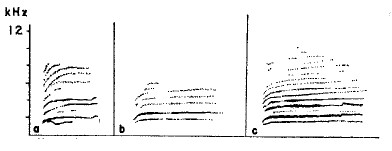
\includegraphics[width=\columnwidth]{figures/sonagraph1}
\caption{Alarm calls of Lawrence's, Lesser, and American Goldfinches
  (\textit{Carduelis lawrencei}, \textit{Carduelis psaltria} and
  \textit{Carduelis tristis}. From Coutlee 1971, Animal Behavior
  19:559.}
\label{fig:sonagraph1}
\end{figure}

\begin{figure}[t]
\centering
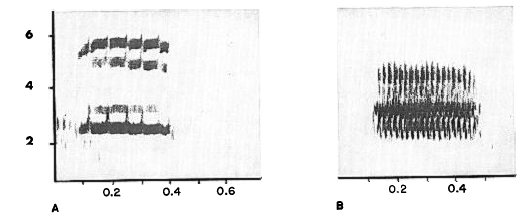
\includegraphics[width=\columnwidth]{figures/sonagraph2}
\caption{The calls of the Varied Thrush \textit{(Ixoreus
    naevius)}. From Martin 1970, Condor 72:453.}
\label{fig:sonagraph1}
\end{figure}

While originally bioacoustic data was recorded onto wax cylinders, for
most of the 20th century, audio was recorded onto analog magnetic
tapes.  These tapes were capable of storing large amounts of data, and
allowed researchers to more easily record the sounds of animals in the
field and the lab.  Analog audio tapes were supplemented by the
introduction of Digital Audio Tapes (DAT) by Sony in 1987.  However,
one limitation of both of these forms of storage is the long time it
takes to seek to a particular place on the tape, due to the linear way
that they store data on tape.

It has only been in recent years that computer hard drives and RAM has
become able to store the large amounts of data that sound represents.
This represents another quantum leap for the field of bioacoustics, as
it allows for large amounts of audio data to be quickly accessible,
and for this data to be indexed and stored in databases and analyzed
by computers.  The field of Music Information Retrieval experienced a
similar blooming in the early 2000's, when computer storage and
computational power became great enough to store and analyze the data
of songs.  The field of bioacoustics is just starting to show similar
growth, and the use of tools from the field of Music Information
Retrieval (MIR) on bioacoustic data has shown great promise.

However, many of the tools developed for MIR are not well adapted for
the study of bioacoustic data.  When studying recorded songs, there is
often a large amount of well-curated meta-data for each song, For
example, when classifying songs based on genre, the artist, song
title, genre, record label and many other forms of data are available,
and boundaries between songs are clearly marked, and are often in
individual files.  Music often come pre-segmented into songs, which
often have identifiable sections including verse and chorus, as well
as lower level features such as beat and tatum that facilitate
analysis by computers.  In addition, most work in MIR has been on
songs that were professionally recorded in a studio environment.

In bioacoustics, this is often not the case, and in the cases of large
bioacoustic databases, recordings are often taken from a single
location, and how close animals are to the recording devices can
change dramatically during a recording.  There are often also many
sources of other sound in the recording, from environmental noise like
wind, to human produced noise like from boats or cars. Also, in many
cases there are a variety of different animals making sound in a
recording, and these sounds can overlap each other.  While some
bioacoustic recordings are well segmented, such as those of the
recordings of bird songs from the Cornell Lab of Ornithology, in many
cases of continous recordings, the locations of the bioacoustic sounds
are not localized in time, and these recordings must be annotated and
segmented before they can be analyzed.

In most studies of bioacoustics to the current time, individual
researchers record the sounds of the animals that they are interested
in studying.  In the process of doing the recording, they make notes
and record other kinds of metadata about the audio they record.  The
amount of audio that is typically analyzed is of the range of hundreds
to a few thousand recordings.  Even in larger studies such as those by
Harald Yurk on the vocalizations of Orcas, the dataset is of the order
of 1000 recordings.  These recordings are typically analyzed on a
single computer using software such as Raven \cite{ravenpro}, a
powerful tool for the study of bioacoustic data produced by the
Cornell Lab of Ornithology.  This software allows researchers to
record, import, view, analyze and annotate recordings and provides
ways to export the annotations to other programs that can be used to
further analyze the audio.  It works best with shorter audio files,
although large files can be read in and viewed using a paging
metaphor, where sections of several minutes of audio are visualized at
a time.

In recent years, the larger storage and computational capacity of
computers has inpsired researchers to analyze larger and larger
collections of bioacoustic data.  Much of the historical audio
recordings are present on audio tapes, and using high-throughput audio
digitization facilities, this data has begun to be transferred to
digital form.  At the University of Victoria, we have previously
described a project called The Orchive \cite{sness2008} where we have
digitized over 20,000 hours recordings from the Orcalab research
facility, stored originally on 45 minute long analog audio cassette
tapes.  These recordings contain large numbers of the vocalizations of
Orcas (\textit{Orcinus orca}) along with other species of marine
mammals.

Another project that collects large amounts of recordings of animals
is the Alberta Biodiversity Monitoring project (ABMI), a project setup
by the Alberta Government to monitor the biodiversity of ecosystems
across the province.  Every summer, researchers are sent to a grid of
over 1700 sites across the province, where they visually make note of
plant and animal species they encounter.  At the same time they are
doing this, they set up a stereo microphone and record 30 minutes of
audio from the site.  During the following fall and winter, a set of
researchers are employed to listen to these recordings and annotate
individual birds in the recording.  These annotations are then used to
determine the changes in biodiversity in the environment.  This
process of annotating birds is done using a simple audio visualization
tool (typically Audacity \cite{audacity}), along with a combination of
Excel spreadsheets, websites that contain examplars of birdsong of
different species, and other web based and electronic resources.

With the advent of computers that can store this large amount of data,
even more ambitious efforts have recently begun to collect continous
data including audio.  Two of these projects are the closely related
VENUS and NEPTUNE ocean observatories, part of Ocean Networks Canada.
In these projects, permanent undersea observatories that are directly
connected via cable links to land collect continous data, including
salinity, pressure, echo sound data, video and audio.  This data
streams in from 6 different observatories, and in the case of audio
data, in many of the locations, multiple channels of high sample rate
audio are collected.  This project has already collected thousands of
hours of audio, and is planned to collect data for the next 25 years.

The advent of very large bioacoustic databases of tens or hundreds of
thousands of hours presents problems to currently existing tools.
Even in the case of the 45 and 30 minute recordings from the Orchive
and ABMI projects, current tools have some issues with allowing
researchers to quickly load the audio, view it, and quickly navigate
around within and between these files.  In addition, the storage space
required for these large audio collections makes it impractical for
researchers to have the whole collection on a local computer.  In the
case of the Orchive, the entire dataset takes about 20TB of disk space
when stored as uncompressed audio files.

The MIR tools used to analyze this audio are also impractical to use
on a single computer, the time it takes to analyze the audio, and the
amount of storage space makes it impractical to analyze large
collections of audio data on a single computer.  It is also important
for researchers to be able to collaborate on these large scale
projects, to share their annotations, audio data, and the raw results
of their analysis with colleagues.  In order to do this, one possible
approach would be to use a web-based system, where the individual
researcher can connect to a large server based system that presents
the data to them in an easy to use form, allows them to make and share
annotations, and connects to large amounts of computing resources for
them to perform audio feature extraction, machine learning and other
forms of analysis on their data.
 
Web-based software has been helping connect communities of researchers
since its inception.  Recently, advances in software and in computer
power have dramatically widened its possible applications to include a
wide variety of multimedia content.  These advances have been
primarily in the business community, and the tools developed are just
starting to be used by academics. We have been working on applying
these technologies to ongoing collaborative projects that we are
involved in \cite{sness2008}. By leveraging several new technologies
including HTML5/Javascipt, Node.js and Python we have been able to
rapidly develop web-based tools.  Rapid prototyping and iterative
development have been key elements of our collaborative
strategy. Although our number of users is limited compared to other
areas of multimedia analysis and retrieval, this is to some degree
compensated by their passion and willingness to work closely with us
in developing these tools.


\subsection{Relevance of this work}

An important aspect in the design of a tool to support collaborative
work is to consider what user communities will use the tool.  In the
case of the Orchive, there are a number of different scientific
communities that will be using this tool and the data this tool
provides access to.  The primary scientific community that will
benefit from this work will be cetacean biologists.  In order to study
the rich archive orca vocalizations that have been recorded by
Orcalab, researchers must currently travel to Hanson Island, search
through the lab books and incidence reports to find which recordings
contain the data they are interested in, locate the physical cassette
tape corresponding to this recording, and then either manually listen
to the tape, or perhaps digitize the tape and analyze it in the
computer.  Each researcher typically then keeps the annotations and
data generated from this procedure themselves, if future researchers
want to obtain this data for further analysis, they must first be
aware of the fact that this researcher has the data, and then request
it from them.  With the distributed collaborative system we have
designed, not only can these biologists easily listen to any recording
in the entire archive from any internet connected computer in the
world, and compare different recordings, they can also add their
annotations to the system.  These annotations can be either private or
public, if they are for use in a publication, after the article has
been accepted for publication, the researcher can make their private
annotations public.  These researchers are less interested in the
details of audio feature extraction and machine learning algorithms,
and are instead more focused on asking biologically informed
questions, like dialect change in cetacean call repertoire
\cite{deecke00}.

Another scientific community that will receive benefits from this
archive are the developers of bioacoustic algorithms.  These
scientists are typically computer scientists with interests in Music
Information Retrieval and bioacoustics.  This archive represents a
site where researchers can get large amounts of high quality and
uniformly collected data.  Researchers interested in bioacoustic
algorithms have different goals and skill sets from cetacean
biologists, for example, many have extensive knowledge of Digital
Signal Processing and audio feature extraction algorithms.  This
system should be flexible and powerful enough to allow these
researchers to ask questions that are relevant to them.  The required
features for this group of users include allowing them to choose
different audio feature extraction algorithms, and to then take the
resulting data and run it against a variety of machine learning
algorithms in as flexible a manner as possible.

Another group of scientists that have expressed interest in the
Orchive are Environmental and Conservation scientists. A research
question particular interest is the effect of boat noise
\cite{foote04_orca_boat_noise} on cetaceans and on the marine
environment in general.  For these researchers, the data they will be
most interested in is the frequency and nature of orca vocalizations,
and the intensity and spectral characteristics of boat noise
\cite{holt09_orca_speaking_up}.  There are large differences in the
intensity and frequency content of boat noise depending on the type of
boat that creates it, speed pleasure craft often create a high pitched
noise that quickly moves away, tug boats have a lower pitched sound
and take a long time to move through an area, and cruise ships make a
loud and distinctively high pitched sound.  Analyzing the effects of
these various types of boat noise will help researchers to establish
guidelines for boat noise as it affects this sensitive population of
marine mammals \cite{doksaeter09_orca_herring_feeding}.

Another group of scientists that this work will benefit are those
studying the social organization of whale communities
\cite{bigg90_orca_genealogy}.  There have been studies that
investigate the transmission of culture in orca societies
\cite{deecke00} and have found evidence of this through the
examination of dialect change.  In a similar vein, other studies have
investigated social learning \cite{janik00_orca_social_communication}
in communities of orcas.  With a large database such as this, more of
these type of studies will be made possible in the future.

Another large and difficult problem domain that requires the skills of
researchers from many different fields is the investigation of orca
vocalizations.  The whale species \emph{Orcinus orca}, commonly known
as Killer Whales \cite{ford00_book_killer_whales}, are large toothed
whales found around the world, in places as far afield as Antarctica
and Alaska\cite{estes09_orca_alaska_decline}.  There are three
distinct types of Orcas, Transients, Residents and Offshores, each of
which have different feeding behaviours and different styles of
communication.  The vocalizations of orcas are complex and diverse,
and consist of a wide variety of vocalizations, which include
echolocation clicks, tonal whistles and pulsed calls \cite{deecke00}.

Around Vancouver Island there are two distinct communities of Orcas,
the Northern Residents, which have a range north of Campbell River,
and the Southern Residents, which spend time around Victoria.  Orcalab
is a research station located on Hanson Island, a small island up near
the top of Vancouver Island, directed by Dr. Paul Spong and Helena
Symonds and which studies the Northern Resident population of Orcas.
Orcalab has been recording Orca song for over 20 years, and has
amassed a huge archive of over 20,000 hours of audio on magnetic
cassette tapes.  In a collaboration with them, we are digitizing and
analyzing this huge and rich archive in a project called "The
Orchive".

In this paper, we will examine the combination of three components of
distributed cognition to help work on the problem of analyzing orca
vocalizations:

- Collaborative technologies to enable distributed cognition between
expert users in with potentially diverse domain knowledge

- The use of machine learning algorithms to provide technologies for
Intelligence Augmentation

- The use of large numbers of people from the general public in a
crowdsourcing methodology to mine through and annotate large databases
of information

Our goal is to create a system that enables distributed cognition
between these three facets, allowing expert users to collaborate,
giving them advanced machine learning algorithms to help them analyze
data, and in cases where datasets are enormous, using the power of
crowdsourcing to pore through large datasets.  In this paper we
describe an application of this approach to the problem of analyzing
the orca vocalizations.

The main motivation behind our work has been creating better
interfaces for interacting with the Orchive \cite{tzanetakis07} a
large archive of audio recordings of Orca vocalizations.  There are
stable resident populations of \textit{Orcinus orca} in the northwest
Pacific Ocean, and some of these populations \cite{ford00} are found
near Hanson Island, off the north tip of Vancouver Island in
Canada. Orcalab is a research station that has been recording audio of
these Orca populations since 1972 \cite{deecke99}. They have amassed a
huge archive of more than 20,000 hours of audio recordings collected
via a permanent installation of underwater hydrophones.

Most of existing work in the automatic analysis of Orca calls has
focused on detection and classification rather than retrieval. A
real-time system with low computational requirements for the detection
of Orca vocalizations is described in \cite{Luke2010771}. Annotation
bootstrapping is a technique used to classify/segment hydrophone
recordings into three broad categories: voiceover, background, and
vocalizations \cite{ness08}.

Our work was influenced by two publications that described different 
representations and methodologies for the classification of Orca
calls. Orca vocalizations consists of well-defined, discrete calls
with tonal signal components. They can be characterized by the pulse
rate contour of the goal which can be viewed as analogous to the pitch
contour of a speech or monophonic music signal. A method for computing 
acoustic similarity between pulse rate contours (normalized so that
they all have the same duration) using the discriminative error of a
Artificial Neural Network is described in
\cite{deecke99}. 

Dynamic time warping (DTW) is a technique for measuring the similarity
of two sequence that many vary in time. It mostly known in the context
of speech recognition \cite{sakoe78} but it has found applications in
many areas including video, motion and DNA sequence analysis. The use
of DTW to compute the similarity between two pulse rate contours in
the context of Orca calls has been explored in
\cite{brown07_orca_dtw}. In that work, a similarity matrix is
calculated containing all the DTW alignment costs between pairs of
pulse rate contours. This similarity matrix is then subsequently used
to calculate clusters which are then compared the ground truth call
labeling to assess the feasibility of call classification using this
approach.

\section{Scope of this work}
\label{section:introduction:scopeOfThisWork}

The fields of Music Information Retrieval (MIR), Visualization and
web-based Human Computer Interaction (HCI) are each vast topics in
their own right, not to mention the application areas of
Ethnomusicology and bioacoustics.  So as to make the present work
tractable, we will focus on three very specific problems and will
apply a carefully selected subset of some of the tools in MIR,
Visualization and HCI to help us in developing solutions for these
areas.

In the field of the analysis of bioacoustic signals from
\textit{Orcinus Orca} vocalizations, we will use tools from MIR,
including Fast Fourier Transforms (FFT) to analyze and display
spectrograms, along with tools such as Mel-Frequency Cepstral
Coefficients (MFCC), average zero crossing rate, and spectral
centroid, along with many other such tools, to help us visualize and
analyze orca vocalizations.  We will be also using techniques from the
fields of Visualization and HCI, including the micro-macro view,
draggable panes, multi-resolution browsing, tagging and the layered
presentation of data.

We will use many of these same tools in the analysis of audio from
chant traditions around the world, and will in addition be using
techniques such as Fundamental Frequency Estimation and Dynamic Time
Warping.

In the area of the analysis of large music collections, we will use
many of the previous tools, including the FFT and MFCC coefficients to
extract features from the songs, and will primarily be using the
technique of Self-Organizing Maps to reduce the dimensionality of the
high dimension spaces created by feature extraction to two dimensions.


%%%%%%%%%%%%%%%%%%%%%%%%%%%%%%%%%%%%%%%%%%%%%%%%%%%%%%%%%%%%%%%%%%%%%%%%%%%%%%%%
%%%%%%%%%%%%%%%%%%%%%%%%%%%%%%%%%%%%%%%%%%%%%%%%%%%%%%%%%%%%%%%%%%%%%%%%%%%%%%%%
%% Chapter - Related Work
%%%%%%%%%%%%%%%%%%%%%%%%%%%%%%%%%%%%%%%%%%%%%%%%%%%%%%%%%%%%%%%%%%%%%%%%%%%%%%%%
%%%%%%%%%%%%%%%%%%%%%%%%%%%%%%%%%%%%%%%%%%%%%%%%%%%%%%%%%%%%%%%%%%%%%%%%%%%%%%%%

\startchapter{Related Work}
\label{chapter:relatedWork}

In this thesis, we are interested in exploring approaches to allow
scientists to view, annotate and analyze large bioacoustic databases.
The study of bioacoustics has a long and rich history, and in the
first section of this chapter, we will present a brief summary of the
history of bioacoustics in general, and will then focus our attention
on previous work done in analyzing the vocalizations of the species
\textit{Orcinus orca} and provide an extensive review of the
literature on this topic.  We will then provide a brief introduction
to the analysis of vocalizations of the taxonomic class Aves, also
known as birds.  The mechanisms of sound production by birds is
extremely diverse, and is an extremely large literature devoted to the
study of the vocalizations of birds, so in this work we will only
attempt to provide a general overview of the literature in this field.
One of the primary motivations in studying large bioacoustic databases
is for the monitoring of the biodiversity of ecosystems, and we will
provide a detailed overview of the work done in the use of
bioacoustics to study changes in biodiversity.  We will also provide a
brief introduction to the field of Acoustic Ecology, and will show how
the research into this field has informed this work and how it relates
to studies of biodiversity.

In the following section, we will provide an overview of the
literature on the use of audio feature extraction to generate features
suitable both for the visualization of bioacoustic data, and for the
use of machine learning algorithms.  We will first provide a brief
history of the use of waveform based methods for visualization of
sounds, and will proceed to the use of spectral based methods,
including sonograms, spectrograms and measures derived from
spectrograms, including Mel-Frequency Cepstral Coefficents and other
descriptions of spectra.  We will then provide a brief overview of the
field of pitch detection, in which algorithms primarily use the
autocorrelation of a time based representation of sound, and of the
use of these methods in the study of bioacoustics.  We will then
examine the use Machine Hearing algorithms based on models of the
human peripheral auditory system, these algorithms typically first use
a filterbank to model the function of the cochlea, followed by a
strobed temporal detection system to model the medial superior olive
brain center, which provides an autocorrelation-like output for each
channel of the filterbank.  We will review literature on the use of
the output of this system, the correllogram, and it's use for the
recognition of sounds.

In the following section, we will present a literature review of
papers on the use of machine learning algorithms on the output of
audio feature extraction algorithms to analyze sound.  Although this
is a relatively new field of study, the literature on this subject is
vast, and we will focus primarily on the use of machine learning
algorithms in the study of bioacoustics, as distinct from the study of
music and other forms of audio.  One approach to classifying sounds is
the use of Dynamic Time Warping, an approach used in the analysis of
human speech, and which has had success in the study of
biacoustics. We will briefly examine the use of older methods such as
tree building algorithms and Gaussian Mixture Models and other machine
learning algorithms.  We will then focus our attention on the use of
Support Vector Machines for audio classification.  We will then
examine the use of Self-Organized Maps (SOM) for generating
2-dimensional representations of collections of audio that are
amenable for navigation by scientists.  SOMs are based an approach
similar to artifical neural networks, and we will examine the use of
artificial neural networks (ANN) to study audio.  In recent years, a
rexamination of the properties of real networks of neurons in living
systems has shown that these systems typically do not work with the
continuous, real valued model of traditional ANNs, but instead have
discrete signals that can be more accurately modelled as a sparse
representation.  Vector Quantization is a recent approach to the study
of sparse representations of audio, and we will examine the literature
of the use of this method, along with other methods that use a sparse
reprentation of audio.  We will finally provide a review of the
literature on recent developments in the tranformation of audio
features into a discrete form based on an alphabetic structure that
are amenable to analysis by tools from bioinformatics.  The approach
of Symbolic Aggregate Approximation (SAX) is one such approach, and we
will examine the use of these types of algorithms to the study of
large collections of data.

In order to allow scientists to listen to, view and perform analysis
on these large collections of audio, the use of computer based tools
is a necessity.  In the past, researchers in bioacoustics would
analyze their data with programs on a single computer such as Raven
and MATLAB.  We will provide only a brief search of the vast
literature on the use of computer based tools to view, annotate and
analyze audio.  In ideal situations, these tools provide for
Intelligence Augmentation (IA), in which computer based tools do not
replace human intelligence, but instead augment, or improve it.  This
stands in contrast to the concept of Artificial Intelligence, where
tools that produce information independently of humans are used, with
the ultimate end of replacing the need for human intelligence.  IA
instead acknoledges that computers and humans have different cognitive
strengths, and that for certain complex tasks, an optimal system would
combine the best aspects of human and computer intelligence.  We will
examine the literature for evidence of tasks that benefitted from the
use of IA, and will draw parallels between these systems and the
system described in this thesis that allows scientists to view,
annotate and analyze large bioacoustic databases.

One of the largest hurdles in the study of large bioacoustic databases
is their vast size, the small number of researchers studying these
databases, and the messy nature of these databases.  In order to
assist scientists with large, the use of citizen science and
crowdsourcing has been used for many years, with approaches as diverse
as the collection of word use for the Oxford English Dictionary, the
use of far-flung citizen scientists to aid Linnaeus with the study of
taxonomy, to the work of Dr. Fred Urquhart in the study of monach
butterfly migrations.  In recent years, the use of the internet has
enabled many more ways for interested members of the public to help
scientists study difficult problems, and we will provide a brief
summary of the literature on this topic.  In this thesis, we present a
simple matching game to allow citizen scientists to assist us in the
classification of audio, in a paradigm we call Serious Casual Games.
We will examine the literature on the use of gamification on the study
of complex phenomena and what aspects of gamification have shown the
most promise in previous studies.

\section{Bioacoustics}
\label{section:relatedWork:bioacoustics}

Humans have used sound to identify animals from time immemorial, some
of the earlist extant literature comes from Aristotle.  In On the Soul
\cite{aristotleA} he describes how animals make sound, and notes that
while some sounds are produced by the ``impact of the inbreathed air
against the windpipe'', there are many other mechanisms by which
animals produce sound.  In The History of Animals \cite{aristotleB},
he describes a wide variety of sounds made by animals, from the ``low
hiss'' of the tortise, the ``peculiar croak'' of the frog, to the
``squeak and moans'' of a dolphin.

Bioacoustics is a scientific field of study that combines the fields
of biology and acoustics.  Although humans have used the sounds of
animals to identify and track them for many years, one of the first
researchers in this field was Ivan Regen who in 1925 systematically
studied the sounds of insects \cite{zarnik29}.  In the later half of
the 20th century, advances in electronic means of recording and
producing sound dramatically increased the breadth and scope of the
field of bioacoustics.  In recent years, the application of the
computational tools used in Music Information Retrieval have further
extended the possibilities of analyzing sound from biological sources.

\subsection{Orcas}

Another large and difficult problem domain that requires the skills of
researchers from many different fields is the investigation of orca
vocalizations.  The whale species \emph{Orcinus orca}, commonly known
as Killer Whales \cite{ford00_book_killer_whales}, are large toothed
whales found around the world, in places as far afield as Antarctica
and Alaska\cite{estes09_orca_alaska_decline}.

There is a considerable, but not immense, literature on the study of
the bioacoustics of \textit{Orcinus orca}, also known as the Killer
Whale.  One of the earliest studies was described by a paper in 1967
by Singleton and Poulter \cite{singleton67} in which a detailed
spectral analysis of the calls of captive Killer Whales in which a
digital approach using a Fast Fourier Transform was used to produce an
spectrogram of short regions of audio.  This study examined pulsed
calls, and made reference to work by Watkins \cite{watkins67} in which
an analysis of pulsed calls was made.  These pulsed calls were
identified by Watkins to be short pulses of tones, and he provided a
detailed analysis of the spectral qualities of these tones, noting
that when studying pulsed calls, the nature of the pulses has a strong
impact on the spectrogram, and gives rise to a banded structure, and
that the distance between the bands gives the repeat rate of the
pulses, this is also known as the Side Band Interval (SBI).  In later
work, especially the catalog of orca vocalizations by Ford
\cite{ford87}, the SBI is one of the primary quantities used in
classifying orca calls.  

The structure of the sound producing organs in odontocetes in general
was described in detail by Cranford \cite{cranford96} who found that
the tissues responsible included a structure that resembled lips and
was made of connective tissue, a cartilaginous blade, a stout ligament
and an array of air sacs made of soft tissues.  This sound producing
organ is capable of producing two sounds at once in a process known as
biphonation.  They noted that the sounds that could be produced
included clicks, whistles, and a sound that was the combination of
both, a pulsed call that could contain both a Lower Frequency
Component (LFC) and Upper Frequency Component (UFC).  In later papers,
\cite{cranford00} \cite{cranford06}, they described this sound
producing organ in more detail.  Brown \cite{brown08} did a study of
the mathematical implications of this pulsed biphonation, extending
the earlier results of Watkins \cite{watkins67}

A paper in 1982 by Dahlheim and Awbrey \cite{dahlheim82} provided a
classification of the sounds of captive killer whales, these whales
had been taken from British Columbia, and a number were identified to
be Northern Resident Killer Whales (NRKW), which makes it very relevant to
this thesis.  In this paper, they describe 11 different categories of
sounds, these are upscreams, downscreams, creaks, whines, whistles,
tones, buzzes, ricochets, click bursts, chatter and seesaw.  In this
paper they note that from the different vocalizations, they are able
to classify individuals by oceanarium with high accuracy.  

An extremely detailed investigation of the vocalizations of the killer
whales off the coast of British Columbia was carried out in a series
of papers by John Ford \cite{ford82} \cite{ford83} that described
the group-specific dialects this population.  In 1987 Dr. Ford
published a large catalog of the pulsed calls of the Northern Resident
Orcas \cite{ford87}.  In this hugely important resource, he used a
systematic nomenclature to describe a catalog of approximately 78
different calls with 24 different subtypes.  The calls were labelled
starting with the letter ``N'' for the Northern Residents, in contrast
to calls from the Southern Residents which were prefixed with the
letter ``S''.  The calls were numbered according to the time that they
were first encountered, starting with N1.  The recordings were made
into Sonagrams using a Kay Electric company sonograph, and the Side
Band Intervals were measured with an electronic digitizing tablet.
This call catalog remains the primary resource for researchers who
wish to study orca calls, and it was hugely relevant to the research
in this thesis.

The calls in this call catalog were examined in more detail in a paper
in 1989 by Ford \cite{ford89}.  In this paper, the vocalizations of
NRKW are divided into three categories, ``clicks'', ``whistles'' and
``pulsed calls''.  The clicks were short pulses of sound that were
typically made in series, with a variable duration of between 0.1ms
and 25ms, and could range in repetition rate from a few pulses per
second to over 300 per second.  These clicks were identified to be
primarily of use in echolocation.  Orcas do considerable amounts of
echolocation to navigate, locate other group members and locate prey
\cite{barretlennard96}.  Whistles were the second type of sound, and
are a single narrow band tone with little or no harmonic structure.
He noted that these whistles were between 1.5kHz and 18kHz and ranged
in duration from 50ms to 12 seconds.  These whistles were of widely
varying character and did not fall into distinct structural
categories.

The third type of call is the pulsed calls, and these are the primary
calls of interest both in the work of Ford and others, and also of
this thesis.  They are of a pulsed nature as described above, that is,
they have a central tone that is rapidly pulsed with abrupt and
pattern shifts between pulse rates.  Pulses typically had repetition
rates of between 250-2000Hz, and a primary energy of between 1 and
6kHz.  He noted three categories of pulsed calls, discrete, variable
and aberrent calls.  Discrete calls had distinctive structural
characterictics and were repetitive, variable calls were modified
versions of these discrete calls, and aberrent calls were clearly
based on discrete calls, but were heavily modified.  In this paper, he
studied the amount of these three classes of calls in different
behavioural circumstances, that of foraging, travelling, resting,
socializing and beach rubbing, and found that more variable and
aberrant calls occurred during socializing and beach-rubbing.  He also
did a transition state matrix of the different call types and found
clear evidence that certain calls were more likely to be followed by
other calls.  The most striking of these was the N7/N8 pair of calls,
in which an N8 call was always preceeded by an N7 call.  This paper is
very relevant to this thesis in that it presents a theoretical
structure for classifying orca calls and for the study of their
vocalizations.  Although it describes results from a large amount of
data, the number of recordings in the orchive is even larger, and
testing the hypotheses stated in this paper with a larger dataset
could be enlightening in the study of orca calls.

Orcas from different parts in the world also have discrete calls that
are diverse, and a study by Parijs \cite{parijs04} on Norwegian Killer
Whales found that none of the calls recorded matched those with those
of a previous call catalog \cite{strager95}.


- Discrete call repetoires are thought to be mainly to promote group
cohesion and to coordinate intragroup activities \cite{ford89}
\cite{ford91}.

- Dolphin signature whistles function as cohesion calls when a social
group is separated \cite{janik98} \cite{watwood05}

- Resident orcas increase use of family specific calls after calves
are born \cite{weiss06} particularily between mothers and their
dependent offspring.

- Call type matching in vocal exchanges \cite{miller04}

- Discrete calls are at an amplitude that far exceeds the intra-group
separation of members \cite{miller06}, and likely function in
inter-group communication. 

- Orcas change their call behaviour in the presence of other groups of
whales \cite{weiss06} increasing the number of matriline-specific,
variable and aberrent calls, and decreasing the number of low arousal
calls.  The calls also changed more when a different subclan was in
the area, and might play a role in coordination of inter-group
activity.

Janik \cite{janik99} did a study on the classification of dolphin
whistles using humans versus an algorithmic approach and found a
greater probability of humans to identify signature whistles than
algorithmic based approaches.  This is highly relevant to this thesis
in that it highlights the importance of using external validation in
studying vocalizations, and the serious casual game interface allows
researchers to easily create new experiments for humans to identify
calls.  These results can then be compared with algorithmic based
approaches to validate their performance.  Recent work by Janik and
King et al. \cite{king2013} suggests that the use of vocal copying
plays an an important role in the social behaviour of dolphins, and
that dolphins can learn the vocalizations of other dolphins.

In a recent paper by Yurk et al. \cite{yurk10} they note that due to
vocal difference between clans, acoustic monitoring is a good way to
monitor populations of orcas, and identified 7 different pods of
whales.  There have been other studies of marine mammals with fixed
hydrophones including humpback whales \cite{norris99}, bowhead whales
\cite{cummings85}, blue whales \cite{stafford98} and killer whales
\cite{morton02}.  In this study, the hydrophone was manned by a single
observer (Michael Brittian) who did the recordings of the different
pods.  In this thesis we describe a system that could be used for the
automated detection and recording of orca calls, thus allowing more
sites to be observed and the reduction of human effort.

However, most of the work in analyzing orca vocalizations has been
painstakingly done by hand, sometimes using audio cassettes and expert
knowledge of orca vocalizations, and sometimes by digitizing
vocalizations into a computer and then analyzing spectrograms.  It
would be of advantage to the field to be able to apply these
algorithms to a large dataset and provide collaborative visualization
tools to explore it.

\subsection{Orcas - Algorithms}

For a number of years, computers have been applied to the study of
orca vocalizations.  One early work \cite{deecke99} used neural
networks to determine similarity between orca vocalizations.  In this
paper, they found that neural networks were able to predict similarity
between calls with an accuracy comparable to that of expert human
listeners.  Another algorithm that has been applied to this problem
domain is that of Dynamic Time Warping
\cite{brown06_orca_dtw}\cite{brown07_orca_dtw}.  In these two papers,
Brown et al. investigate the use of DTW for calculating similarity
between two orca vocalizations and find that this algorithm performs
very well.  DTW is used frequently in the field of MIR, and this
thesis discusses its use as applied to chant traditions from cultures
around the world in another chapter.

The mathematical foundations of the pulsed vocalizations by orcas have
also been studied \cite{brown08_orca_pulsed_math}.  In this paper,
formulas for their spectra are rigorously derived from the basic
formulas of Fourier analysis.  This paper describes in detail the
complex spectra that are able to produced by orcas and the biological
foundations that underlie them.

Another mathematical method that has been used to describe orca
vocalizations is the Hilbert-Huang transform, which has been shown
\cite{adam06_orca_hilber_huang} to have advantages over using
traditional Fourier based methods of calculating spectra.

One important pitfall in the automated classification of orca
vocalizations \cite{deecke06} is that there exist non-linearities in
sound perception in all animals, including orcas\cite{nummela99}.
When designing tools and algorithms to study these vocalizations, it
is important to recognize the differences between human and orca
perception of sound.


- Individual orcas tend to match call types produced by other group
members \cite{miller04} and this can assist group cohesion
\cite{miller02} and allow individual recognition \cite{miller07}.

- Low Frequency Component (LFC) with fundamental frequency between 80 and
2.4kHz

- Some also contain HFC with fundamental frequency between 2 and 12kHz
\cite{hoelzel86}

- Necessary to track each component of the frequency

- Also, two or more different orcas can be making calls at one time,
need to separate them \cite{ford87}

- Cultural transmission of language \cite{deeke99}

Considerable individual variability of orca vocalizations \cite{miller00}
\cite{nousek06} \cite{parijs04}.  

In a paper by Miller and Bain \cite{miller00} they noted that discrete
calls always have a LFC, and often end in a ``terminal note'', a
relatively short feature at the end of a call separated by the rest of
the call by a rapid change in the slope or frequency of the LFC.
Within a call type, they found that the UFC was highly stereotyped.
The similarity between call types correlated highly with the how often
the matrilinear units (MU) associated with one another, which was from
previous work by Bigg et al. \cite{bigg90}.



- Recordings often have large amount of boat noise.  Many orcalab
recordings are done over VHF which makes their quality similar to
telephone calls, thus algorithms that are designed to handle noise are
useful \cite{wang00}

- However, these algorithms often depend on harmonic structure, and
for many orcalab recordings, the orcas are distant from the
hydrophones, and there is not much harmonic structure present

- Two different ways to classify vocalizations \cite{deecke99}

   - Statistical - Look at properties of the pitch track and do
   statistics on them.  Only assess physical properties of the signal
   and not how they are perceived.

   - Perceptual - Have humans (or animals) listen to the pitch and
   classify them.  Observer bias.  Dolphins have a more advanced
   peripheral auditory system than humans \cite{au00}

   - In this paper, they present results from the sidewinder
   algorithm which uses autocovariance of FFT with a neural network.
   They compare these results to those by humans who had no knowledge
   of orca vocalizations. 

   - Algorithm performed well even with poor SNR.  

   - Advantages
     - Uses more points that other analyses that just use a few points
       on the pitch contour (min, max, etc. \cite{au00})

   - Disadvantages
   	 - Had problems when noise had a harmonic component
   	 - Cannot be applied to broadband or pure tone signals
     - Computationally expensive compared to other approaches
     - Suggest that it can be used in combination with other algorithms.
	 - Does not take amplitude into consideration
	
   - Neural net and human approach gave similar results.

- Pulsed calls so the highest energy is not always contained in the
first, second or third harmonics \cite{watkins67}

A recent investigation into the calls of Orcas off the coast of
Scotland by Deecke et al. \cite{deecke11} found that a herring eating
group of whales produced pulsed calls like those produced by the NRKW,
and that one of their calls appeared to have a herring herding
function.

In a paper by Au et al. \cite{au04} the echolocation clicks of orcas
were measured and analyzed in detail.  They found that the clicks were
of very short duration, between 80 and 120us in duration, and had a
bimodal broadband distribution, with one peak at 45kHz to 80kHz and
one from 35 to 50kHz, 97\% of the time.  They estimate that orcas
would be able to detect salmon at a distance of 100m even in the
presence of heavy rain noise.  They also mention that boat noise is of
a different character than rain and wind noise, and the impact of boat
noise on echolocation is unknown.  This paper is of relevance to this
thesis in that in the data in the Orchive, there are many such
recorded echolocation clicks, and a deeper understanding of these
clicks and how orcas adapt their echolocation behaviour in the
presence of noise could be a useful contribution to the literature.
This theme of the impacts of noise on Orca communication can also be
found in \cite{holt09}, where the impacts of noise on the Southern
Resident Killer Whale (SRKW) population is examined.  In this paper
they found that when boat noise increased by 1dB, orcas raised their
volume of their calls by 1dB.

Janik \cite{janik99} studies the use of three different algorithmic
techniques to compare dolphin whistles.  The first is based on an
algorithm by McCowan \cite{mccowan95} that first normalizes the length
of each call, and then takes 20 points along its length as independent
variables.  These then used as input to a Pearson product-moment
correlation matrix which then gives a similarity measure between pairs
of whistles, which was then subjected to Principal Component Analysis
to reduce the number of colinear variables.  These values were then
used as input to a k-means clustering algorithm.  This paper also used
two cross-correlation based methods one that used the
cross-correlation of two signals using a method described by Khanna et
al. \cite{khanna97}, and the other that used the same
cross-correlation, but instead took the absolute difference in
frequency every 5ms.

Considerable work has gone into the identification of dolphin
signature whistles in the last two decades \cite{sayigh90}.  A recent
paper by Janik et al. \cite{janik12} presents a new method for
comparing dolphin whistles called SIGnature IDentification (SIGID)
which uses the observations of human listeners followed by bout
analysis, in which they found that they could reliabily detect
individual dolphins in recordings of groups of dolphins.  This
research is explained in greater depth of the Ph.D. thesis of King
\cite{king12} where the use of signature whistles as vocal labels
amongst other topics is examined.  This is of relevance to the current
thesis in that we present an extensible computer system that would
allow researchers to conduct the human study portion of the SIGID
system using citizen scientists.

Other interesting work on dolphin communication is presented in a
recent paper by Janik \cite{janik2013cognitive} in which the
capability of dolphins to refer to objects and other dolphins using
referrents and their ability to understand syntatic structure is
reviewed.  This paper is of relevance in that orcas are of the same
taxonomic family as are dolphins, and could possibly share some of
their cognitive abilities.


One approach to determining the fundamental frequency of a
vocalization is to manually trace spectrogram by hand using
appropriate software, for example, in Watwood et al. \cite{watwood04}
the Matlab software suite is used to this end.  A recent paper by
Shapiro et. al \cite{shapiro06} uses this same approach.  While this
approach is appropriate for small datasets, it is most likely
untenable for the multi-thousand hour datasets explored in this
thesis.

The crosscorrelation of spectrogram images was explored in early work
by Clark \cite{clark87}.  In this work, songs of the swamp sparrow
were transformed into spectrograms, and a straightforward
cross-correlation of the spectrograms was used to get a quantitative
measure of their similarity.  They obtained good classification
results, from about 73\% for one song type to 92\% for another.

Another approach that has been used is to select peak frequency from
sliding power spectrum followed by manual correction to remove octave
errors \cite{buck93} \cite{janik94}.  In previous work in our lab
\cite{ness08} this approach was also used by hand with Matlab, and in
our software suite, we have functionality that allows a user to select
a wide variety of paramters for pitch determination algorithms that
brings this same functionality to a web-based interface.

One of the most useful algorithms for determining the pitch contours
of orca calls is the sidewinder algorithm which uses autocovariance
for each spectral slice where the peaks are at multiples of the
spacing of frequency bands \cite{deeke99}.  This algorithm is
particularily appropriate to sounds that are of a pulsed-tone nature.
These sounds are composed of a pure tone that is pulsed at a specific,
and perhaps varying, rate.  A spectrogram of such tones has many bands
\cite{watkins67} around a central frequency, with the most energy
occuring near the frequency of the tone, and not in the lower
harmonics, as is in the sounds of many instruments.  The sidewinder
algorithm is similar to the spectral autocorrelation method for human
speech tracking \cite{lahat87}.

A similar algorithm is the Discrete-Logarithmic Pitch Detection
Algorithm DLFT-PDA \cite{wang00}.  The DLFT-Makes reliable estimations
of pitch and temporal change of pitch from harmonic structure by
correlating DLFT spectra from adjacent frames to give reliable
esimates fundamental frequency change.  It uses Dynamic Programming to
create smooth pitch track.  However, two drawbacks of this algorithm
are that it performs poorly with low SNR and cannot track multiple
calls by multiple animals.  It was shown to be a a versatile pitch
tracking algorithm in recent work by Shapiro et al. \cite{shapiro09}

Another approach that takes advantage of the banded structure of
pulsed calls is an FFT based comb filter method with Dynamic Time
Warping \cite{brown06}.  In this approach, an upsampled FFT of a sound
is produced, and this FFT is then analyzed with a series of comb
filters with equally spaced frequency bands to isolate the harmonic
structures of different repetition rates. This was explored in
\cite{brown06} and then in more detail in \cite{brown07}.  This
approach takes as input a pitch contour as determined by a pitch
determination algorithm, and can take multiple pitch tracks to model
sounds in which an LFC is combined with an UFC.  The DTW algorithms
they explored included the Ellis, Sakoe-Chiba, Itakura and
Chai-Vercoe.  These vary in the way that the cells are computed, for
example in the Chai-Vercoe method, there is explict handling of
insertions and deletions in the cost matrix.  These algorithms can be
compared to those used in global-sequence alignment algorithms.  They
found that they could get 90\% agreement with perceptual data, and
represented a severe test of DTW.  Used both the LFC and UFC
components.

Another approach used an Artificial Neural Network (ANN) image of
spectrogram transformed into an image of data points then normalized
and transposed into a vector of points points which was the input to
the ANN \cite{gaetz93}.  Looked at distinguishing calls from each
other in one experiment, and whales from each other in another, both
experiments gave excellent classification accuracy on a small dataset.

A paper by Adam \cite{adam06} discusses the use of the Hilbert-Huang
Transform (HHT) for analyzing the sounds of marine mammals.  They
mention that the FFT is limited to the Heisenberg Uncertainty
principle, and that time and frequency resolutions must be chosen by
the investigator, and relate that the HHT does not suffer from this
drawback.  They say that FFTs are best suited for analysing harmonic
signals, but not for click sounds, while the HHT is better suited for
this.  They provide results that show the effectiveness of the HHT
over the FFT, especially in the case of clicks where when the ratio
between the maximum of the energy when a click is present to that when
the click is absent is approximately 20:1 with the FFT and is
approximately 100:1 with the HHT.

Another approach using FFTs to classify whale calls can be found in
Oswald et al. \cite{oswald03} where they used a multivariate
discriminating function analysis for classifying whale vocalizations.
In this paper they examine the use of different upper frequency limits
(20, 24, 30 and 40kHz) and different variables for each call,
including beginning and ending frequency, minimum and maximum
frequency, duration, number of inflection points, number of steps and
if harmonics were present from the fundamental frequency of each
whistle.  They got fairly poor classification accuracy (37\% at 24kHz)
using a multivariate approach with crossvalidation, but their detailed
analysis of using these different parameters was quite useful.  With a
more sophisticated statistical treatment and a dataset larger than the
484 whistles from 29 recording sessions, it might be possible to obtain
higher classification accuracy.


Another more recent approach by Deecke included the use of the
Adaptive Resonance Theory (ART) neural network, a network similar to
the Self-Organizing Map approach in that it is an unsupervised
approach using a neural-net like foundation, however, in the ART
algorithm, if a new pattern is found that is sufficiently different
from existing patterns, it becomes the reference pattern for a new
category.


- Multi-pitch estimation of mixtures of signals \cite{klapuri08}
\cite{fujihara12}

- Automatic music transcription \cite{benetos12}

- Yin algorithm

The use of a Self-Organized Map for analyzing animal vocalizations
\cite{placer06} found that they could identify individual acoustic
elements in sounds, and allowed alarm calls to be classified with 91\%
accuracy.  They also mention that when the topological structure of
the SOM was transformed into a string representation, that different
digrams and trigrams were found to be associated with alarm calls for
different predators.  This paper is relevant to the current work in
that it shows one possible way that SOMs can be used to analyze audio,
and the framework described in this paper allows researchers to use a
SOM to analyze their own data.  It also provides another method for
turning audio data into a sequence of symbols, similar to the symbolic
approximation algorithms described in this thesis.

Another way to classify audio features is to use the Pearson product
moment correlation which was used in Watwood et al. \cite{watwood04}
to classify the vocalizations of bottlenose dolphins.  The main
advantage of this technique are that it takes into account the
differences that are lost when whistle loops are normalized in time,
it also ignores absolute frequency and bandwidth information.  By
doing so, it makes loops that have monotonic changes in frequency
appear more similar even if they are considerably different in
absolute frequency.

\subsection{Birds and Biodiversity}


The paper first describes the importance of monitoring and measuring
of the sounds of animals and insects.  In the natural habitat, the
sounds of animals can be used to determine how many animals are in a
location and what species these animals are, and can help scientists
measure the biodiversity of a location, and how this biodiversity
changes over time.  There is recent interest in this field of study
\cite{wimmer2010} \cite{seuer2008} as a method for determining the
biodiversity changes in regions over time.  The authors then say that
an automated system for detecting insects would also be useful from a
commercial point of view,

The paper then goes on to say that in laboratory settings, it would
also be advantageous to have an automated system that could segment
and classify recordings.  Currently this task often requires
researchers to annotate hundreds of recordings by hand, which is a
very time intensive task.  As a scientist who has done many hours of
hand annotating of large sound archives, I can attest to the
difficulty and time-consuming nature of this task.

The authors then say that there are many problems with current methods
of detecting, segmenting and classifying the sounds and vocalizations
of animals.  Current methods require researchers to manually annotate
recordings and to generate a large corpus of data to be used by
classification algorithms.  These algorithms often have a large number
of tunable parameters, some of which can be automatically determined
from the large amount of training data, and some which have to be
manually explored by the researchers.  In addition, many of these
algorithms are computationally expensive and cannot be deployed in the
field.  I have found these facts to be true in my own research, and I
appreciate the fact that the authors spend time discussing the
problems faced by researchers studying bioacoustics.

The use of bioacoustics for the study of species in the Amazon is
presented in \cite{riede93}, in which a system for doing rapid surveys
of species in forested areas are presented.  Challenges of doing
surveys of species via visual surveys include the complexity of tree
architecture, the inaccessibility of species, rarity, excellent
camouflage, and cryptic and noctural lifestyles.  In addition, the
visual identification of species is labour intensive, costly and is in
increasingly short supply.  Many of these species can be heard, but
cannot be seen, and this paper presents the challenges and advantages
of using sound to identify these species.  The challenges include the
lack of resources of audio recording exemplars of these species,
however mentions that there are many new projects devoted to the
collection of sound samples from species.  The advantages include the
fact that many of these species have evolved so that their sounds are
distinct from each other, and are thus amenable to study from
acoustial fingerprinting.  This paper is of relevance to the current
work as it shows that the use of bioacoustics for monitoring diversity
of species can be a useful approach.

An early paper in this field is ``Monitoring biodiversity: analysis of
Amazonian rainforest sounds'' \cite{riede93} in which the author
sketches out an approach to detecting organisms by looking at the
amplitude spectra of their vocalizations.  He describes a case study
carried out in the Amazon where the target organism is a species of
cricket.  The author notes that by analyzing the amplitude spectra of
this species, clusters of peaks were detected that had definite
characteristics, specifically they had repetitive signals in the 4kHz
and 9kHz bands that had a comb-like structure and had pulse rates of
between 20 and 80 pulses per second.  He hypothesizes that by using
neural network techniques, it would be possible to develop a system
that automatically classifies these recordings.

An approach for doing a rapid survey of biodiversity is presented in
\cite{sueur08}.  In this work, the bioacoustic signatures of
individual species are not identified, but rather an approximation of
the biodiversity of a region is calcuated using an acoustic entropy
index, in which the temporal entropy of a Hilbert-Huang transform of
the sound is used to estimate the number of species in a region.  From
actual recordings from Borneo they find that the acoustic entropy has
a logarithmic relationship to the number of species in a region.  In
addition, they find that in regions where environmental impacts have
occurred, that spectral profiles show a higher dispersion of peaks of
amplitude along the frequency axis.  This paper is of some relevance
to our work, however in this thesis we are primarily interested in the
actual identification of individuals and species from the sounds they
make.

An excellent review of the field of using automated sound recording
and analysies for doing surveys of birds was done by Brandes in 2008
\cite{brandes08}.  In this paper, two broad categories of automation
are examined, the first being the automated recording of bird sounds,
and the second being the automated analysis of these sounds.
Different types of hardware recording devices are discussed, as well
as different types of microphones suitable for this task.  Of more
direct relevance to this thesis is the section which discusses the
automated analysis of bird songs, and divides bird vocalizations into
5 distinct categories, which are constant frequency, frequency
modulated whistles, broadband pulses, broadband pluses with varying
frequency components and segments with strong harmonics.  They make
note that different audio feature extraction and machine learning
algorithm pairs are necessary for obtaining features from these
different kinds of vocalizations, for example, for pulse to pulse
duration features are useful and neural networks have been shown to be
useful and for sounds with frequency modulated whistles or segments
with strong harmonics, cepstral coefficients combined with dynamic
time warping and hidden markov models have shown their effectiveness.
This paper relates to this thesis in that we have developed a system
to allow for the many hours of recordings captured by recording
devices to be viewed and allows for a variety of audio feature
extraction and machine learning algorithms to be applied to audio.

Three traditional methods of measuring bird biodiversity are stop
counts, in which an observer travels a specific distance and stops to
record all instances of birds, point counts, \cite{bardeli10} and
mapping of breeding territories.  A recent paper \cite{frommolt08}
describes how the use of bioacoustic approaches have assisted these
traditional methods.  Important ways that automated recordings can
help is that the recording can be done in the absence of an observer,
which can be of benefit in ecologically sensitive areas.  In addition,
noctural and low vocal activity can be studied with the use of long
duration recordings.  This paper describes several actual bioacoustic
recording studies and talks about the advantages of this method.  This
paper is of direct relevance to the current work in that it shows how
bioacoustic recordings can directly benefit studies in biodiversity.

In this same conference, a paper by Bardeli et. al \cite{bardeli08}
describes the use of automated algorithms to detect bird songs in the
results described above.  In it, the song of the caffinch is detected
using a three step procedure, in which first all end segments of a
song are detected, then element repetition frequencies in a given time
window before the song end are estimated, and finaly each combination
of end sequence with repeated segments that are in a range consistent
with caffinch sounds are reported.  Dynamic time warping is used to
detect the end segments, and an autocorrelation based method is used
for the estimation of repeat frequencies.  In our system, we allow for
both the use of Dynamic Time Warping and Autocorrelation based
methods, and would support the studies carried out in this paper.

In \cite{bardeli10} the authors describe a system for performing
censuses of bird populations using automated methods.  Their method
uses DSP based techniques that take advantage of both frequency
content and temporal characteristics of bird songs, and describe
filter chains that were optimized to detect two bird species, the
Eastern bittern and Sevi's warbler.  Both of these methods are finely
tuned to the individual characteristics of these two songs, for
example, the song of the Eastern Bittern has a dominant frequency of
150Hz which is repeated in a specific temporal pattern.  They perform
frequency analysis of the audio and use a peak picking algorithm at
150Hz to detect candidate events, and then use an autocorrelation
based method to lower the number of false positives.  Although they
show good results for these two species in isolation, they admit that
scaling this method up to cases with multiple bird species would be
difficult, and that the presence of noise in recordings is also a
challenging for their method and could introduce false positives.

The field of Acoustic Ecology studies how living beings and the
environment interact through sound \cite{wrightson2000introduction}.
It was founded in the 1960's by Barry Truax \cite{truax2001handbook}
and primarily involves the recording of soundscapes of environments
sometimes combined with the creation of artistic pieces
\cite{westerkamp2002linking} that include these soundscapes.  These
environments often include the sounds of animals and are often
recorded in natural environments from wildernesses
\cite{smith2004listening} around the world
\cite{feld1994ethnomusicology}.  In the literature, there is often an
overlap of the term acoustic ecology when talking about animals
\cite{nowacek2005acoustic} \cite{kroodsma1996ecology}, and although
this is a distinct field from the acoustic ecology of Truax, there is
considerable overlap in the methodology and the practice of deep
listening of these two fields \cite{redstrom1998acoustic}.


\section{Audio feature extraction}
\label{section:relatedWork:audioFeatureExtraction}

Audio feature extraction is the first step in classifying audio using
machine learning algorithms.  

- Waveform

- Spectrum
	- MFCC

Mel-Frequency Cepstral Coefficients \cite{Logan00melfrequency} (MFCC)
have been widely used for this purpose.  MFCCs have also been used in
bioacoustics, and have been used to classify insect sounds
\cite{leqing11}, birds \cite{changhsing07} and orca calls
\cite{ness08}.  We have investigated the use of MFCC values for
classifying calls from the orca call catalog, and results using these
with a variety of machine learning techniques are described below.  In
future work we would like to try to use MFCC or other forms of
spectral data as input to our symbolic approximation algorithm.

Mel-Frequency Cepstral Coefficients
\cite{Logan00melfrequency} (MFCC) have been widely used for this
purpose.  MFCCs have also been used in bioacoustics, and have been
used to classify insect sounds \cite{leqing11}, birds
\cite{changhsing07} and orca calls \cite{ness2008}.  In this work we
also use MFCCs, but supplement them with other audio features
including Centroid frequency, Rolloff frequency, Flux, and
Zero Crossings.


- Pitch detection


A commonly use audio feature that is often used is an estimate of the
fundamental frequency (F0) or pitch, one well known algorithm for this
is the Yin algorithm \cite{cheveigne02}.  This algorithm is primarily
an autocorrelation based approach, which means that it takes the audio
signal and convolves it with itself.  The peaks in this convolution
then correspond to harmonics in the signal, and with noise free data
with harmonics that strictly decrease, the lowest peak is the
fundamental frequency.  With audio that does not fit this strict
definition, there are many cases where the lowest peak is not the
fundamental frequency, one example is if odd harmonics are
systematically lower than even harmonics, and another is if there is
substantial noise in the data.  The Yin algorithm makes several
modifications to simple autocorrelation to overcome these issues.

Praat \cite{boersma93} is another modern pitch determination
algorithm, it is an autocorrelation based approach that provides good
robustness by making the assumption that pitch is stable in a small
window.  It uses a Hanning or Gaussian window to smooth the edges of
the window to be analyzed and finds peaks that occur after the zero
lag peak.  It has been shown to work well for estimatating the pitch
of human speech signals.

Another algorithm that is useful for studying sounds with multiple
pitches is the SACF algorithm of Tolonen and Karjalainen
\cite{tolonen00}.  In this algorithm, the signal is decomposed into
two frequency bands (below and above 1000 Hz) and amplitude envelopes
are extracted for each frequency band. The envelope extraction is
performed by applying half-wave rectification and low-pass filtering.
The envelopes are summed and an enhanced autocorrelation function is
computed so that the effect of integer multiples of the peak
frequencies to multiple pitch detection is reduced.

Another modern pitch detectors that we used in previous work is the
SWIPEP \cite{camachophd} algorithm which determines clusters of
pitched and unpitched sounds.  This algorithm was less appropriate to
use on the mostly pitched discrete calls that orcas produce, but could
be of benefit when studying bird calls that contain both pitched and
unpitched regions.

A different methodology of doing audio feature extraction was explored
in the paper ``Distributed audio feature extraction for music''
\cite{bray05}.  In this paper the authors use a dataflow architecture
for distributed audio feature extraction on a set of networked
computers.  A dataflow architecture allows users to connect small
processing algorithms in a graph like network and to then use this
constructed network to transform input data into a desired type of
output data.  A simple example of a Marsyas network would take audio
samples from a file on disk, multiply them by a number and output them
to another file on disk, which would have the effect of increasing the
volume (loudness) of the file.  However, most of the commonly used
algorithms in Marsyas are complex feature extraction and machine
learning algorithms.  Marsyas was an existing software platform that
used this dataflow architecture, and this paper explored the use of
dataflow architectures on networked computers.  One of the important
contributions of this paper was that the optimal vector size of data
to send from one computer to the other was influenced by the network
settings of their ethernet routers, but in their case a 256 size
vector provided the best speed.  Results are also presented to show
that by using a Collection Partitioning Adaptive algorithm the authors
were able to get the best utilization of their cluster.  This
algorithm splits up the files to be processed and adaptively sends
more jobs to the computers that have completed their past jobs
quickest.  The authors also note that it is very simple to port an
existing Marsyas network to this distributed framework, and there is
indeed current efforts ongoing to do this in an automated fashion.

One serious drawback of this framework is the large amount of disk and
network traffic that is generated by the producer nodes on these
system, the authors point out that the maximum number of worker
computers that could be served by one dispatcher computer was only
four.  This makes sense because of the large amount of data generated
in many of the intermediate steps in the audio feature extraction
pipeline.  The authors propose a system of hierarchical dispatchers
and workers to solve this problem.

For many interesting tasks in realtime computer generated music and
analysis of music in performance situations this type of system would
be very useful, for example, one dispatcher could communicate with a
number of workers each of run a different type of Machine Learning
algorithm and where the results are then collated.  However, for the
present task of analyzing huge collections of audio that is already on
disk in a batch fashion, the architecture in distributed Marsyas
likely would need further work to be of much use.



In ``Overview of OMEN''\cite{McEnnis2006}, McEnnis, McKay and Fujinaga
describe their system called OMEN (On-demand Metadata Extraction
Network), a system that shares many commonalities with the OpenMIR
system we describe in this paper.  The main issue their system aims to
overcome is copyright problems that researchers encounter when they
want to legally extract audio features from songs.  In the strictest
legal sense, each researcher must purchase their own version of a song
in order to do any kind of audio science on it.  This becomes
prohibitive in the age of the Million Song Dataset.  In the OMEN
system, a coalition of libraries creates a network of systems that
host the raw audio data of the song, but only send back to the
researchers the specific audio features that they are interested in.
Another interesting aspect of this system is that they propose to use
the unused computing cycles of library browsing computers to be a grid
computing resource for doing their audio feature extraction.

One big difference is that their system is primarily based on Java,
where my system uses Java, but is primarily based on Python, C++ and
Javascript.  In many ways, the Java ecosystem is enticing for building
server applications, and several times in this project we considered
doing feature extraction in jMIR, the Java Music Information Retrieval
library that the OMEN system happens to use.  However, there are
considerable barriers to getting a productive Java development and
production system installed and maintained.

Their system has a Master Node computer that coordinates all tasks,
Library Nodes that coordinate tasks for a single library and Worker
Nodes that perform feature extraction.  In their system, Library Nodes
store the raw data and distribute it to the Worker Nodes.  One
possible sub-optimal case would be if a single Library Node got
overwhelmed with requests, in this case, it would be challenging to
get other Library Nodes to serve requests to new Worker Nodes.  The
MapReduce framework allows us to sidestep this issue, and by helping
with data locality, allows us to reduce the amount of data sent over
the network.

\subsection{Cochlear Models}

The models of the human auditory system developed by researchers
around the world have a fundamentally different approach in which
audio is filtered by a filterbank cascade that models features of the
human cochlea, the outputs of these filters are then processed by a
mechanism that is modeled on higher levels in the auditory periphery
that take this filterbank audio and generate two dimensional movie
frames that contain both frequency and an autocorrelation axis.  These
frames contain the fine timing information that is utilized by the
human hearing system to separate, localize and identify sounds.

Another type of audio feature extraction that is promising is features
based on models of the auditory cortex \cite{lyon82}.  These
algorithms model the properties of the cochlea and peripheral nervous
system\cite{lyon10}, and have at their core an adaptive filterbank
coupled to a triggered pulse model \cite{waltersphd}.  However, one
issue with these systems is that instead of a 1-dimensional (waveform)
or 2-dimensional (spectral), they lead to a 3-dimensional dataset in
which 2-D audio images change over time, which leads to a very large
amount of data.  Approaches using vector quantization could be used as
an input to our symbolic approximation algorithm in future work.

For my main project, I ported a new model of the human cochlea called
the Cascade of Asymmetric Filters and Resonators (CARFAC) \cite{lyon2011cas}  This model
is the latest in a series of ever more accurate and efficient models
of the human auditory system \cite{lyon82}.  Last summer I was
involved with investigating the performance of the Pole Zero Filter
Cascade (PZFC) model \cite{lyon10} in a variety of audio tasks, where
it performed very well.

- Correllogram

These algorithm 



\section{Machine Learning}
\label{section:relatedWork:machineLearning}

- Machine learning and MIR

- Dynamic Time Warping

Dynamic time warping (DTW) is a technique for measuring the similarity
of two sequence that many vary in time. It is mostly known in the context
of speech recognition \cite{sakoe78} but it has found applications in
many areas including video, motion and DNA sequence analysis. The use
of DTW to compute the similarity between two pulse rate contours in
the context of Orca calls has been explored in
\cite{brown07_orca_dtw}. In that work, a similarity matrix is
calculated containing all the DTW alignment costs between pairs of
pulse rate contours. This similarity matrix is then subsequently used
to calculate clusters which are then compared the ground truth call
labeling to assess the feasibility of call classification using this
approach.  

- Older methods
	- Tree based
	- Gaussian Mixture Model

- Support Vector Machines

Support Vector Machines have been used with song-level features for
automatic tag classification trained at different granularities
(track, album, artist) \cite{mandel-ismir2008}.

- Self-Organizing Maps

Self organizing maps have been used extensively in the visualization
of data for audio based music information retrieval \cite{cooper06}.
They have been used to analyze and organize music archives
\cite{rauber01a} \cite{rauber98a} \cite{rauber98b} \cite{rauber02a},
and to visualize the resulting music collections \cite{rauber03a}
\cite{pampalk04} \cite{rauber02}.  A particularily relvant study was
that of Palmalk in his paper Islands of Music \cite{pampalk03}.  SOMs
have also been used for audio retrieval, browing and constructivist
learning in several papers \cite{cano02} \cite{fruehwirth01}
\cite{honkela00}.  While the previous mentioned studies concentrated
on organizing whole classes of music, SOMs have also been applied to
smaller audio segments, including timbre \cite{toirvainen97},
energy-spectrum \cite{masugi04}, and musical time series analysis
\cite{capinteiro98}.

Self-organizing maps \cite{kohonen95a} are a multidimensional scaling
technique where a high dimension dataset is mapped to a lower,
typically 2-dimensional surface. SOMs and other such dimensionality
reduction tools allow users to visualize data relationships within
complex datasets.  There have been many applications of SOMs in Music
Information Retrieval including work by automatically analyzing and
organizing music archives \cite{rauber01a} \cite{rauber98b},
visualizing music genres \cite{pampalk03}\cite{pampalk03} and music
recommendation \cite{vembu05a}.  Self-organizing maps have been used
in Islands of Music \cite{RPM02} as well as the Databionic
visualization \cite{MUN05}.

- Vector Quantization

A paper highly relevant to our own, yet using very different
underlying audio features and Machine Learning algorithms is ``Sound
retrieval and ranking using sparse auditory representations''
\cite{lyon10} by Dick Lyon and his colleagues at Google.  In this
paper, the authors describe a system designed to help them to create
systems to understand sounds, and they use both a novel audio feature
representation based on models of human hearing combined with a novel
Machine Learning algorithm previously used for image retrieval named
PAMIR (Passive Aggressive Model for Image Retrieval).  In this system,
the data was represented as sparse vectors, which is quite different
from the dense feature vectors commonly used in DSP.  Sparse vectors
have mostly zero values, with just a few non-zero values, and dense
vectors have numbers in almost all their elements.  Sparse vectors are
commonly found in Machine Learning systems that work with text.

In their system, they compare the results of the typical features that
are used in Machine Hearing, the Mel-Frequency Cepstral Coefficients
\cite{Logan00melfrequency} (MFCC) with those of their novel algorithm,
one based on models of the human peripheral auditory system which used
a filterbank called the Pole-Zero Filterbank Cascade (PZFC) and used
this data to make a series of Stabilized Auditory Images (SAIs).
While on one hand the MFCC system outputs a one dimensional vector for
each time slice, producing an image for the sound file when these time
slices are stacked, the SAI system on the other hand generates a two
dimensional vector at each time slice, which can be represented as an
image which can be stacked to form a movie.  The authors describe a
system whereby these images are divided into a number of regions, and
the section of the images that are in these regions are then clustered
based on their similarity using vector quantization to generate a
dictionary using an training set of audio.  This dictionary is then
used to do vector quantization of test audio, and these features are
used as input to the PAMIR system.

PAMIR is a new algorithm for doing mappings from a huge sparse feature
set to a very large query-term set, and was traditionally used in
image recognition \cite{chechik10} to generate tags for images on
Google Image search.  In this context, PAMIR is used to tag SAI images
in order to add tag annotations to sound files.  The authors show
impressive results, with an average precision of 35\% and best
precision at top-1 of 73\%.

This paper is directly relevant to my current paper, and in fact there
are a number of the algorithms in this paper that we want to implement
in my own OpenMIR system.  However, it should be noted that while
these algorithms, specifically the modeling of the auditory cortex and
the SAI model, do show a substantial increase in performance over
traditional techniques, they do come with a substantial performance
hit, and are typically much slower than traditional algorithms since
they often must do an $O(n^2)$ step to calculate the SAI image while
traditional FFT techniques only must do an $O(n(log(n)))$ step.  In
any case, the method of using vector quantization, SAI images and
advanced Machine Learning techniques such as PAMIR shows great promise
in the future in my work.

A paper highly relevant to our own, yet using very different
underlying audio features and Machine Learning algorithms is ``Sound
retrieval and ranking using sparse auditory representations''
\cite{lyon10} by Dick Lyon and his colleagues at Google.  In this
paper, the authors describe a system designed to help them to create
systems to understand sounds, and they use both a novel audio feature
representation based on models of human hearing combined with a novel
Machine Learning algorithm previously used for image retrieval named
PAMIR (Passive Aggressive Model for Image Retrieval).  In this system,
the data was represented as sparse vectors, which is quite different
from the dense feature vectors commonly used in DSP.  Sparse vectors
have mostly zero values, with just a few non-zero values, and dense
vectors have numbers in almost all their elements.  Sparse vectors are
commonly found in Machine Learning systems that work with text.

In their system, they compare the results of the typical features that
are used in Machine Hearing, the Mel-Frequency Cepstral Coefficients
\cite{Logan00melfrequency} (MFCC) with those of their novel algorithm,
one based on models of the human peripheral auditory system which used
a filterbank called the Pole-Zero Filterbank Cascade (PZFC) and used
this data to make a series of Stabilized Auditory Images (SAIs).
While on one hand the MFCC system outputs a one dimensional vector for
each time slice, producing an image for the sound file when these time
slices are stacked, the SAI system on the other hand generates a two
dimensional vector at each time slice, which can be represented as an
image which can be stacked to form a movie.  The authors describe a
system whereby these images are divided into a number of regions, and
the section of the images that are in these regions are then clustered
based on their similarity using vector quantization to generate a
dictionary using an training set of audio.  This dictionary is then
used to do vector quantization of test audio, and these features are
used as input to the PAMIR system.

\section{Auditory Sparse Coding}

The concept of sparsity has attracted considerable interest in the
field of machine learning in the past few years.  Sparse feature
vectors contain mostly values of zero and one or a few non-zero
values.  Although these feature vectors can be classified by
traditional machine learning algorithms, such as SVM, there are various
recently-developed algorithms that explicitly take advantage of
the sparse nature of the data, leading to massive speedups in time, as
well as improved performance.  Some fields that have benefited from
the use of sparse algorithms are finance, bioinformatics, text mining
\cite{balakrishnan2008}, and image classification \cite{chechik2010}.
Because of their speed, these algorithms perform well on very large
collections of data \cite{bottou2007}; large collections are becoming 
increasingly relevant given the huge amounts of data collected and warehoused 
by Internet businesses.

This fine-timing information from the cochlea can be made use of in
later stages of processing to yield a three-dimensional representation
of audio, the stabilized auditory image (SAI)\cite{patterson2000},
which is a movie-like representation of sound which has a dimension of
`time-interval' in addition to the standard dimensions of time and
frequency in the spectrogram. The periodicity of the waveform gives
rise to a vertical banding structure in this time interval dimension,
which provides information about the sound which is complementary to
that available in the frequency dimension.

There is also growing evidence that in the human nervous
system sensory inputs are coded in a sparse manner; that is, only
small numbers of neurons are active at a given time
\cite{olshausen2004}.  Therefore, when modeling the human auditory
system, it may be advantageous to investigate this property of
sparseness in relation to the mappings that are being developed. The
nervous systems of animals have evolved over millions of years to be
highly efficient in terms of energy consumption and computation. 
Looking into the way sound signals are handled by the auditory
system could give us insights into how to make our algorithms more
efficient and better model the human auditory system.

One advantage of using sparse vectors is that such coding allows very fast
computation of similarity, with a trainable similarity measure 
\cite{chechik2010}. The efficiency results from storing, accessing, and doing 
arithmetic operations on only the non-zero elements of the vectors.   
In one study that examined the performance of sparse
representations in the field of natural language processing, a 20- to
80-fold speedup over LIBSVM was found \cite{haffner2006}.  They
comment that kernel-based methods, like SVM, scale quadratically with
the number of training examples and discuss how sparsity can allow
algorithms to scale linearly based on the number of training examples.

In the paper ``Monitoring and Mining Insect Sounds in Visual
Space''\cite{hao12}, Hao et al. describe a novel method for data
mining large databases of insect sounds. 

Campana-Keogh (CK) measure \cite{campana2010} which uses the
concept that two images are similar if one image can be used to
compress the other image. 

\section{Bioinformatics}

The transcription of time series data into a character sequence that
can be consumed by bioinformatics sequence alignment tools is a
nontrivial task.  An attempt towards this goal is Symbolic Aggregate
Approximation (SAX) which was proposed by Lin et al. in
\cite{Lin2003}. The underlying idea of SAX is to parse a time series
using a sliding window and to generate a character sequence that
approximates the signal's normalized slope using a technique called
Piecewise Aggregate Approximation (PAA).  SAX is most useful in cases
where the data is not on an absolute scale.  


\section{Intelligence Augmentation}
\label{section:relatedWork:intelligenceAugmentation}

Although it is a positive thing that this archive of data is now
available in electronic form, what would make it even more useful to
scientists would be the ability to collaborate together on the process
of annotating audio, running experiments and analyzing results.  This
type of work falls under the rubric of Computer Supported
Collaborative Work \cite{bannon91} (CSCW), a field which studies
multiple individuals working together with computer systems.

In this particular case, we have a number of different communities who
have shown interest in this archive, these include Orcalab and its
collaborators, whale biologists, developers of bioacoustic and Music
Information Retrieval algorithms, and the part of the general public
who enjoy listening to whales and might like to help the scientists
who are working on this project.  

As the scientists in this project are located all over the world,
having a system that enables them to work together collaboratively
even though they are separated by large distances will be a worthwhile
challenge \cite{bradner02} \cite{olson00}.  There are a number of
pitfalls that have been identified \cite{grudin88} including the
disparity between who performs the work and who gets the benefits, the
breakdown of intuitive decision-making and the difficulty in
evaluating the application.  To overcome these problems, we are
eliciting feedback at every stage of the design process from
stakeholders, including the members of Orcalab, and we incorporate
this feedback using an iterative development methodology.

Our system uses two types of web based interfaces.  The first are
tools aimed at expert users, and the second are simpler interfaces
designed for crowdsourcing the annotation. There are a number of tools
that experts use to segment and analyze audio and specifically
bioacoustic data.  One of the most popular is Raven
(http://www.birds.cornell.edu/raven), a toolkit developed at the
Cornell Lab of Ornithology.  Our expert based tools have many
similarities to Raven such as the ability to view waveforms and
spectrograms at multiple levels of detail. In addition, our system
tightly integrates the visualization and viewing of data from machine
learning classifiers.  Another tool is the Sonic Visualizer
\cite{cannam10}, which supports a wide variety of waveform and
spectral audio representations. The popular audio program Audacity has
been extended to allow for the annotation of audio data \cite{li06}.
The biggest difference our system compared to these systems is that
the software is all web-based, so users do not have to install a
separate program and can more easily view long audio files and analyze
data across multiple recordings.

The goal of early research in Artificial Intelligence (AI) was to
build independently intelligent agents that could perform cognitive
tasks.  There were a number of approaches to build such systems, some
researchers, such as John McCarthy, chose to build symbolic
manipulation systems where knowledge was represented by formal logic.
Others, such as efforts by Marvin Minsky, instead attempted to combine
several ad-hoc solutions to create an independent agent.  Most of
these systems failed to take into account that in the real world,
intelligent agents, such as people, are embodied, that is they have a
physical form, and this physical body interacts both with other agents
in social interactions as well as with its environment. 

In the 1980's instead of Artificial Intelligence, researchers instead
began to investigate Intelligence Augmentation \cite{fischer92}, where
instead of trying to build intelligent systems that were designed to
replace humans, researchers started building systems that would help
people to solve problems, combining the best of human and artificial
problem solving strategies.  These agents were designed to assist
humans and inherently carried within them the idea that intelligence
was embodied and interacts with people and other artificial agents
through social interactions.

A interesting study was carried out by Sumner \cite{sumner97} and
investigated embedding agents that functioned as critics into a design
environment.  In a critiquing approach, an artificial system
communicates in a dialog with a human, suggesting changes to places
where there are problems with the design.  The system described in
this paper is that of voice menus for a phone-based interface.  The
system is designed by a person or team, and the system critiques the
design in places where the designer has violated previously determined
rule-based constraints.  This work was extended in a subsequent
article \cite{fischer98a} where a system to help designers create
kitchens was described.  One interesting result from these studies was
that designers reacted negatively to being critiqued, and began to
anticipate the response of the system and took steps to avoid being
critiqued.  This highlights the importance of making sure the system
that is built makes the users feel that they are empowered and are
being supported by the system.

In a debate entitle ``Direct manipulation vs. interface agents''
\cite{schneiderman97}, Ben Schneiderman and Pattie Maes debate the
relative advantages of direct manipulation and software agents.
Direct manipulation is described to be user interface techniques where
large amounts of data are presented to the user on the screen at one
time.  Through a user interface with fast feedback (<100ms), the user
navigates through the data.  Software agents, on the other hand, are
described to be long-lived software systems that learn user
preferences and adapt to users, presenting them with data that the
system estimates will be useful to the user.  In this paper, these two
approaches are discussed and contrasted.  It is interesting to note
that by the end of the debate, both sides acknowledge benefits to the
others position, and indeed, as we have seen in the decade since this
debate, systems are being designed that support both direct
manipulation and software agents.  In The Orchive, we are attempting
to design a system that supports both of these paradigms, allowing the
user to directly manipulate large quantities of data, and also provide
software agents that can mediate interactions between users, other
users, annotations from other software agents, and the data.

In the paper ``Distributed intelligence: extending the power of the
unaided, individual human mind'', \cite{fischer06} Fischer provides an
excellent overview of the field of distributed intelligence, relating
it back to work in distributed cognition by Hollan et. al
\cite{hollan00} as well as tying in other concepts, such as those of
Intelligence Augmentation, advanced visualization interfaces that
exploit the power of the human visual system, making user specific
systems, and exploring computing off the desktop, which includes both
large scale and small scale displays.  This paper also explores the
difference between ``Tools for Learning'', which have the goal of
educating the user so that they will be independent of the system and
``Tools for Living'' that help people do things they could not do
themselves.  In The Orchive, we are developing tools to support both
these paradigms, first, to help users learn the calls used by the
orcas, and second, to help more advanced users interact with the data,
allowing them to ask and answer research questions. 

In the paper ``Collaborative, programmable intelligent agents''
\cite{nardi98}, a system that extracts semantic data from documents
using intelligent agents is described.  This paper talks about the
difficulty of creating systems that approximate real intelligence and
instead proposes that that we should investigate what tasks computers
are good for, what tasks people are good for, and how they can best
complement each other.  Their goal is to create a system that works
like a reference librarian, taking imprecise requests from clients and
returning relevant results.  They then present a system called ``Apple
Data Detectors'', which uses a collaborative system to work with the
user to fulfill their requests.

The field of Distributed Cognition studies the social and
environmental aspects of cognition and realizes that thinking is not
just something that happens in isolated minds, but can also take place
in the interactions between minds and their environment.  It was first
formulated into a discrete discipline by Edwin Hutchins, which is
described extensively in his book ``Cognition in the Wild''
\cite{hutchins96} after his research into the native people of Papua
New Guinea and their system of public litigation \cite{hutchins80}.
In a classic paper by Hollan, Hutchins and Kirsh \cite{hollan00}
distributed cognition in different environments is described.  One of
these is on the bridge of a ship, a location where multiple persons
have to work together to accomplish many simultaneous and shared
goals.  In this situation, people work together, sharing information
via intentional and consequential communication and also offload
cognitive tasks to their environment by the use of maps, displays and
other physical objects.

The practice of Cognitive Ethnography \cite{hollan00} is often used to
study distributed cognition.  It studies the cognitive processes that
underlie the work that occurs in an environment, and takes into account
the effect of the social context of the participants as well as the
way the physical world affects the process.  Ethnography is a
methodology in which researchers study a system by making direct
observations in as natural a setting as possible \cite{mcgrath95}.

In the book ``Distributed cognitions: Psychological and educational
considerations'', \cite{salomon97} a number of authors investigate
distributed cognition, and give examples of this in a number of
fields, including daily life and education.  One central theme of this
book is that people think in conjunction or partnership with others
and use tools to help them think.  They also note that it has been
observed that the performance of people in teams supported by
computational tools is often superior to people working alone.  They
then investigate how distributed cognition can be harnessed in the
field of education, with the goal of helping students to learn more
effectively.

There has been a long and fruitful history of the application of
distributed cognition in the sciences.  If one adopts a loose
definition of distributed cognition as thought processes that happen
not just in one individual brain, but are instead distributed through
a community and are mediated by artifacts, the whole history of
science itself, even back as far as Aristotle, has been an example of
distributed cognition.  In the words of Isaac Newton:

 ``If I have seen further, it is by standing on the shoulder of
giants''.

However, recent advances in the understanding of the concept of
distributed cognition from researchers in the social sciences,
combined with advances in computer and communication technology could
dramatically increase the speed, facility and ease of communication
between scientists.  These increases could potentially be
revolutionary changes in certain very difficult problem domains.  In
such domains, the problem itself is too big to be solved by one single
researcher and must instead be solved by teams of researchers with the
aid of artifacts that aid cognition.

There are many different such problem domains that require
collaborations between large numbers of users, three such examples are
high energy physics, genomics research and the study of the
vocalizations of whales.

In the field of particle physics, collaborative software has been used
for a number of years, and indeed, the World Wide Web (WWW) was
developed at CERN by Tim Berners-Lee \cite{bernerslee92}.  The WWW was
developed in order to help physicists collaborate with one another by
creating a ``global information universe''.  One of the primary goals
of the WWW was to enable the sharing of data between researchers.  The
Large Hadron Collider is a new multi-billion experiment at CERN, one
of the goals of which is to find evidence for the Higgs-Boson
\cite{wells09}.  The LHC will generate truly vast quantities of data
and will require enormous processing power \cite{wiebalck03}, because
of this, a huge network of computer systems called ``The Grid'' has
been developed.  This system allows researchers to distribute and
access data and to share computational resources at sites around the
world.  However, perhaps due to the culture in the high-energy physics
community, there has been only a small amount of development of tools
\cite{birnholtz03} to allow people to collaborate with other people
\cite{horn04}.  The Grid was designed to allow researchers to
efficiently access machines, but not for people to collaborate
efficiently with other people.  In an ideal system, these two
communication channels would both be facilitated.

Another area of research that involves large numbers of scientists
working together to solve a large problem was the sequencing of the
human genome \cite{venter01}.  The public effort to sequence the human
genome involved researchers from many different universities in
different countries, and required communication and collaboration
between all of these laboratories in order to coordinate sequencing
efforts.

A paper that describes the nature of communication and collaboration
in the biological sciences is ``Capturing and supporting contexts for
scientific data sharing via the biological sciences collaboratory''
\cite{chin04}.  In this paper the authors talk about the challenges in
sharing data between scientists in the field of biology.  Another
paper \cite{tabard08} describes Prism, a hybrid laboratory notebook
that allows scientists to collaborate together in the solution of
biological problems by using a hybrid electronic laboratory notebook.
This labbook brings together cross-linked streams of data, both
physical and electronic and integrates activity streams from different
users.  In a very recent paper \cite{segal09}, Segal discusses the
challenges faced by software developers in creating systems to allow
scientists to collaborate.  She makes the observation that it is
important for the developers to internalize the contextual structure
with which the scientists communicate in order to make an effective
system.

An interesting paper by Kuchinsky et al. \cite{kuchinsky02} describes
a software tool for creating a synthesis of the complex concepts in
molecular biology, and uses the framework of storytelling to help
scientists make sense of data.  They find that the addition of a
narrative structure to data helps scientists organize, retrieve, share
and reuse biological data.  Most data is transmitted in a dense code
between biological scientists, and by many scientists in general, and
this paper highlights the fascinating idea of using the innate ability
of people to understand stories in order to transmit data between
scientists more efficiently.  We can transmit data from computer to
computer very quickly using codes that are natural to computers, and
it is important to remember that to transmit data to a person, one
should use methods of communication that are natural to people.

\section{Citizen Science}
\label{section:relatedWork:citizenScience}

Citizen science is a process by which members of the public are
involved in a collaboration with professional scientists to collect
and analyze data.  Although it's coinage as a term is rather recent,
it has a well-established history, with one of the earliest examples
being that of Linnaeus who in his Systema Naturae \cite{linnaeus1758}
asked volunteers from the public to send him botanical samples from
around the world for the development of his taxonomical system.  Other
examples include the establishment of a system of amateur weather
observatories across the US by Thomas Jefferson \cite{fiebrich09} and
the Christmas Bird Count \cite{lebaron09} of the Audubon society and
Cornell Lab of Ornithology.

However, in recent years the use of networked computers has
dramatically accellerated the ability for scientists and the public to
collaborate on large scale projects.  The term crowdsourcing refers to
a new type of collaboration where non-specialists help expert
scientists \cite{howe08_crowdsourcing} and has been used to great
advantage \cite{surowiecki05_crowdsourcing} in a number
\cite{bradham08_crowdsourcing} of research programs
\cite{travis08_crowdsourcing}.  One of the most successful examples is
Galaxy Zoo \cite{anze08_galaxyzoo}. Games-with-a-purpose (GWAP)
\cite{vonahn08}, which are computer games that harness the ability of
people to solve tasks in a game setting.  The first GWAP was the ESP
game \cite{vonahn04} in which two users on computers connected to the
internet try to guess words that describe an image.  In ``Game-powered
Machine Learning'' \cite{barrington12}, Barrington, Turnbull and
Lanckiet describe a system that combines Games With A Purpose (GWAP)
with Machine Learning in a framework that they call ``Active Machine
Learning''.  In the paragraphs below, we examine these contributions
in greater detail.

One of the most successful citizen science programs is Galaxy Zoo
\cite{anze08_galaxyzoo}.  In this project, astronomers had collected
images of many thousands of galaxies and wanted to characterize them
by the chiral handedness of their spiral structure, that is, were they
spinning clockwise or counterclockwise?  It was assumed that there
would be an even distribution of these the two chiral hands, left and
right, and any deviations from this would be an important and
surprising result.  Even the most advanced current computer algorithms
are not able to categorize galaxies based on their handedness, but
humans can do this classification easily.  In this paper, the authors
describe their system and results, and present results that indicate
that there is a hint of positive correlation for galaxies nearer than
0.5 Megaparsecs.

Another research program that benefited from crowdsourcing was the
Stardust@home project \cite{mendez06_stardust}.  Stardust
\cite{atkins97_stardust} was a NASA space mission that flew a
spacecraft through the tail of comet Wild 2, collected dust from the
comet and from interstellar matter using an aerogel, and then returned
the satellite to earth.  Comet dust was collected on one side of the
aerogel, and the other side of the aerogel was exposed to interstellar
matter during the entire mission.  The analysis of the particles from
the comet were straightforward due to the high number of particles,
but the analysis of interstellar grains was much more difficult due to
the small size and number of particles.  The Stardust@home project
allowed users from around the world to signup on a website and
interactively view and annotate microscopic images of the aerogel.
There was overwhelming participation by the public, and they were able
to generate results that were useful to the scientists on the project
\cite{atkins97_stardust}.

There have been a number of articles that investigate the benefits of
crowdsourcing.  Hong \cite{hong04_crowdsourcing} presents results that
show that a group of problem solvers with a diverse background can
outperform smaller groups of experts.  This is of interest in the
current work because there are only a very small number of orca
vocalization experts in the world, but there is a large number of
people who are interested in listening to orca calls, as is evidenced
by the traffic on the Orca Live \url{http://orcalive.net} forums.

A recent article \cite{kittur08_crowdsourcing} describes crowdsourcing
with the Amazon Mechanical Turk system, a web based system where
people can sign up to work on small tasks in return for micropayments.
The advantage with using the Mechanical Turk system is that because
people are paid for their work and have to pass a scientist defined
test, the results obtained might be of higher quality.  The drawback
to this system is that the workers must be paid.  Most scientific
projects have limited budgets, and thus this type of solution is often
not practical.

One exciting new development in crowdsourcing is games-with-a-purpose
(GWAP) \cite{vonahn08}, which are computer games that harness the
ability of people to solve tasks in a game setting.  The first GWAP
was the ESP game \cite{vonahn04} in which two users on computers
connected to the internet try to guess words that describe an image.
If both users guess the same word, this word is then added to the tags
to that image, and is also added to a list of forbidden words which
forces people to choose new words to describe an image.  This game has
proven immensely popular, with many millions of tags added to images.
Another such game is Tag-A-Tune \cite{law09}, an input agreement game
that has people add tags to music clips.  These games, and others like
them, exploit the powerful reward system of the human limbic system
and are an excellent way to hold the attention of large numbers of
users and generate high quality data.  The challenge with
games-with-a-purpose is to develop a captivating game experience, but
with time and skill, they perhaps hold the largest potential in terms
of sheer size of population for performing crowdsourcing.

Although many of these projects concentrate on recruiting large
numbers of participants, even small numbers of human volunteers can be
of great use when analyzing bioacoustic data.  Of particular relevance
to this thesis is work done by researchers in cetacean bioacoustics
\cite{ford91} \cite{yurk10} \cite{yurkphd} \cite{dolphinwhistles}
where human volunteers were used to classify orca and dolphin
vocalizations into distinct categories.  These researchers used
different kinds of technology to do this, primarily not with a
computer, but in recent work by Yurk \cite{yurk10} \cite{yurkphd} a
web-based interface was developed to allow volunteers to help classify
vocalizations.  The results by the human volunteers was used to help
evaluate the performance of machine learning algorithms.  This has
direct relevance to the current work in that in this thesis we
describe a system that extends this work by providing an integrated
system where researchers can upload, annotate and create new sets of
classification tasks for humans to perform.  The system that we have
implemented also adds game like elements to hopefully provide greater
engagement of the public along with a concomittant increase in the
amount of data collected.

In ``Game-powered Machine Learning'' \cite{barrington12}, Barrington,
Turnbull and Lanckiet describe a system that combines Games With A
Purpose (GWAP) with Machine Learning in a framework that they call
``Active Machine Learning''.  In this framework, the user is presented
with a set of plausible answers by a Machine Learning system, these
plausible answers are chosen to be as close to the actual answer as
possible, which helps the system train itself on difficult data most
effectively, and also makes the game more fun and challenging to play,
since the answers are so close to each other.  This kind of system
directly inspired the work we describe earlier with GWAP, and how we
are developing a system to let users help us to classify orca calls,
and by using active learning we can help to make this game fun and
challenging.


%%%%%%%%%%%%%%%%%%%%%%%%%%%%%%%%%%%%%%%%%%%%%%%%%%%%%%%%%%%%%%%%%%%%%%%%%%%%%%%%
%%%%%%%%%%%%%%%%%%%%%%%%%%%%%%%%%%%%%%%%%%%%%%%%%%%%%%%%%%%%%%%%%%%%%%%%%%%%%%%%
%% Chapter - Software and Systems
%%%%%%%%%%%%%%%%%%%%%%%%%%%%%%%%%%%%%%%%%%%%%%%%%%%%%%%%%%%%%%%%%%%%%%%%%%%%%%%%
%%%%%%%%%%%%%%%%%%%%%%%%%%%%%%%%%%%%%%%%%%%%%%%%%%%%%%%%%%%%%%%%%%%%%%%%%%%%%%%%

\startchapter{Software and Systems}
\label{chapter:softwareAndSystems}


\section{System Overview}
\label{section:softwareAndSystems:systemOverview}

Given the vastness of this archive, there are certainly many different
tasks that bioacousticians and other scientists might want to do with
it, but one primary obstacle is that the Orchive is currently mostly
unlabelled.  After 4 years, there are approximately 12,000 annotations
in the Orchive, which represents only a few hours of actual annotated
time.  Even with many scientists working on labelling this data, it
would take many person-years to label the entire Orchive.  By using a
combination of expert users and Machine Learning software, it is
possible to train Machine Learning classifiers on expert labelled data
and from there to predict the location of orca vocalizations.  In
order to further add to the training data for the Machine Learning
classifiers, we have also built simple iPad and web based casual games
with a serious intent, which we call serious casual games.  Casual
games are those like the well known Solitare, which take a short
amount of time to play and do not require all the users attention.  By
allowing these citizen scientists to assist us, we are able to collect
larger amounts of data, and to sort through data we have generated
quickly.  In fact, one of the main users of this game software has
been ourselves, we find the game interface a quick and effective way
to label training data.

With these interfaces, we are able to label substantial amounts of
data, but are still far away from labelling the entire 20,000 hour
archive.  In order to do this, researchers have commonly used a
combination of the techniques of Audio Feature Extraction and Machine
Learning to classify audio.  In this paper we will use a combination
of Audio Feature Extraction and Machine Learning to identify sections
of the Orchive where there are clear orca vocalizations that are
distinct and not overlapping with the vocalizations of other orcas and
are relatively free of boat noise. These extracted vocalizations will
then be made available to the scientific community and will also be
used by our lab in future work for answering other scientific
questions about this species.  A system diagram of how this process of
Machine Learning, Expert Interfaces and Serious Casual games works,
please refer to Figure \ref{fig:systemDiagram}.

\begin{figure}
\centering
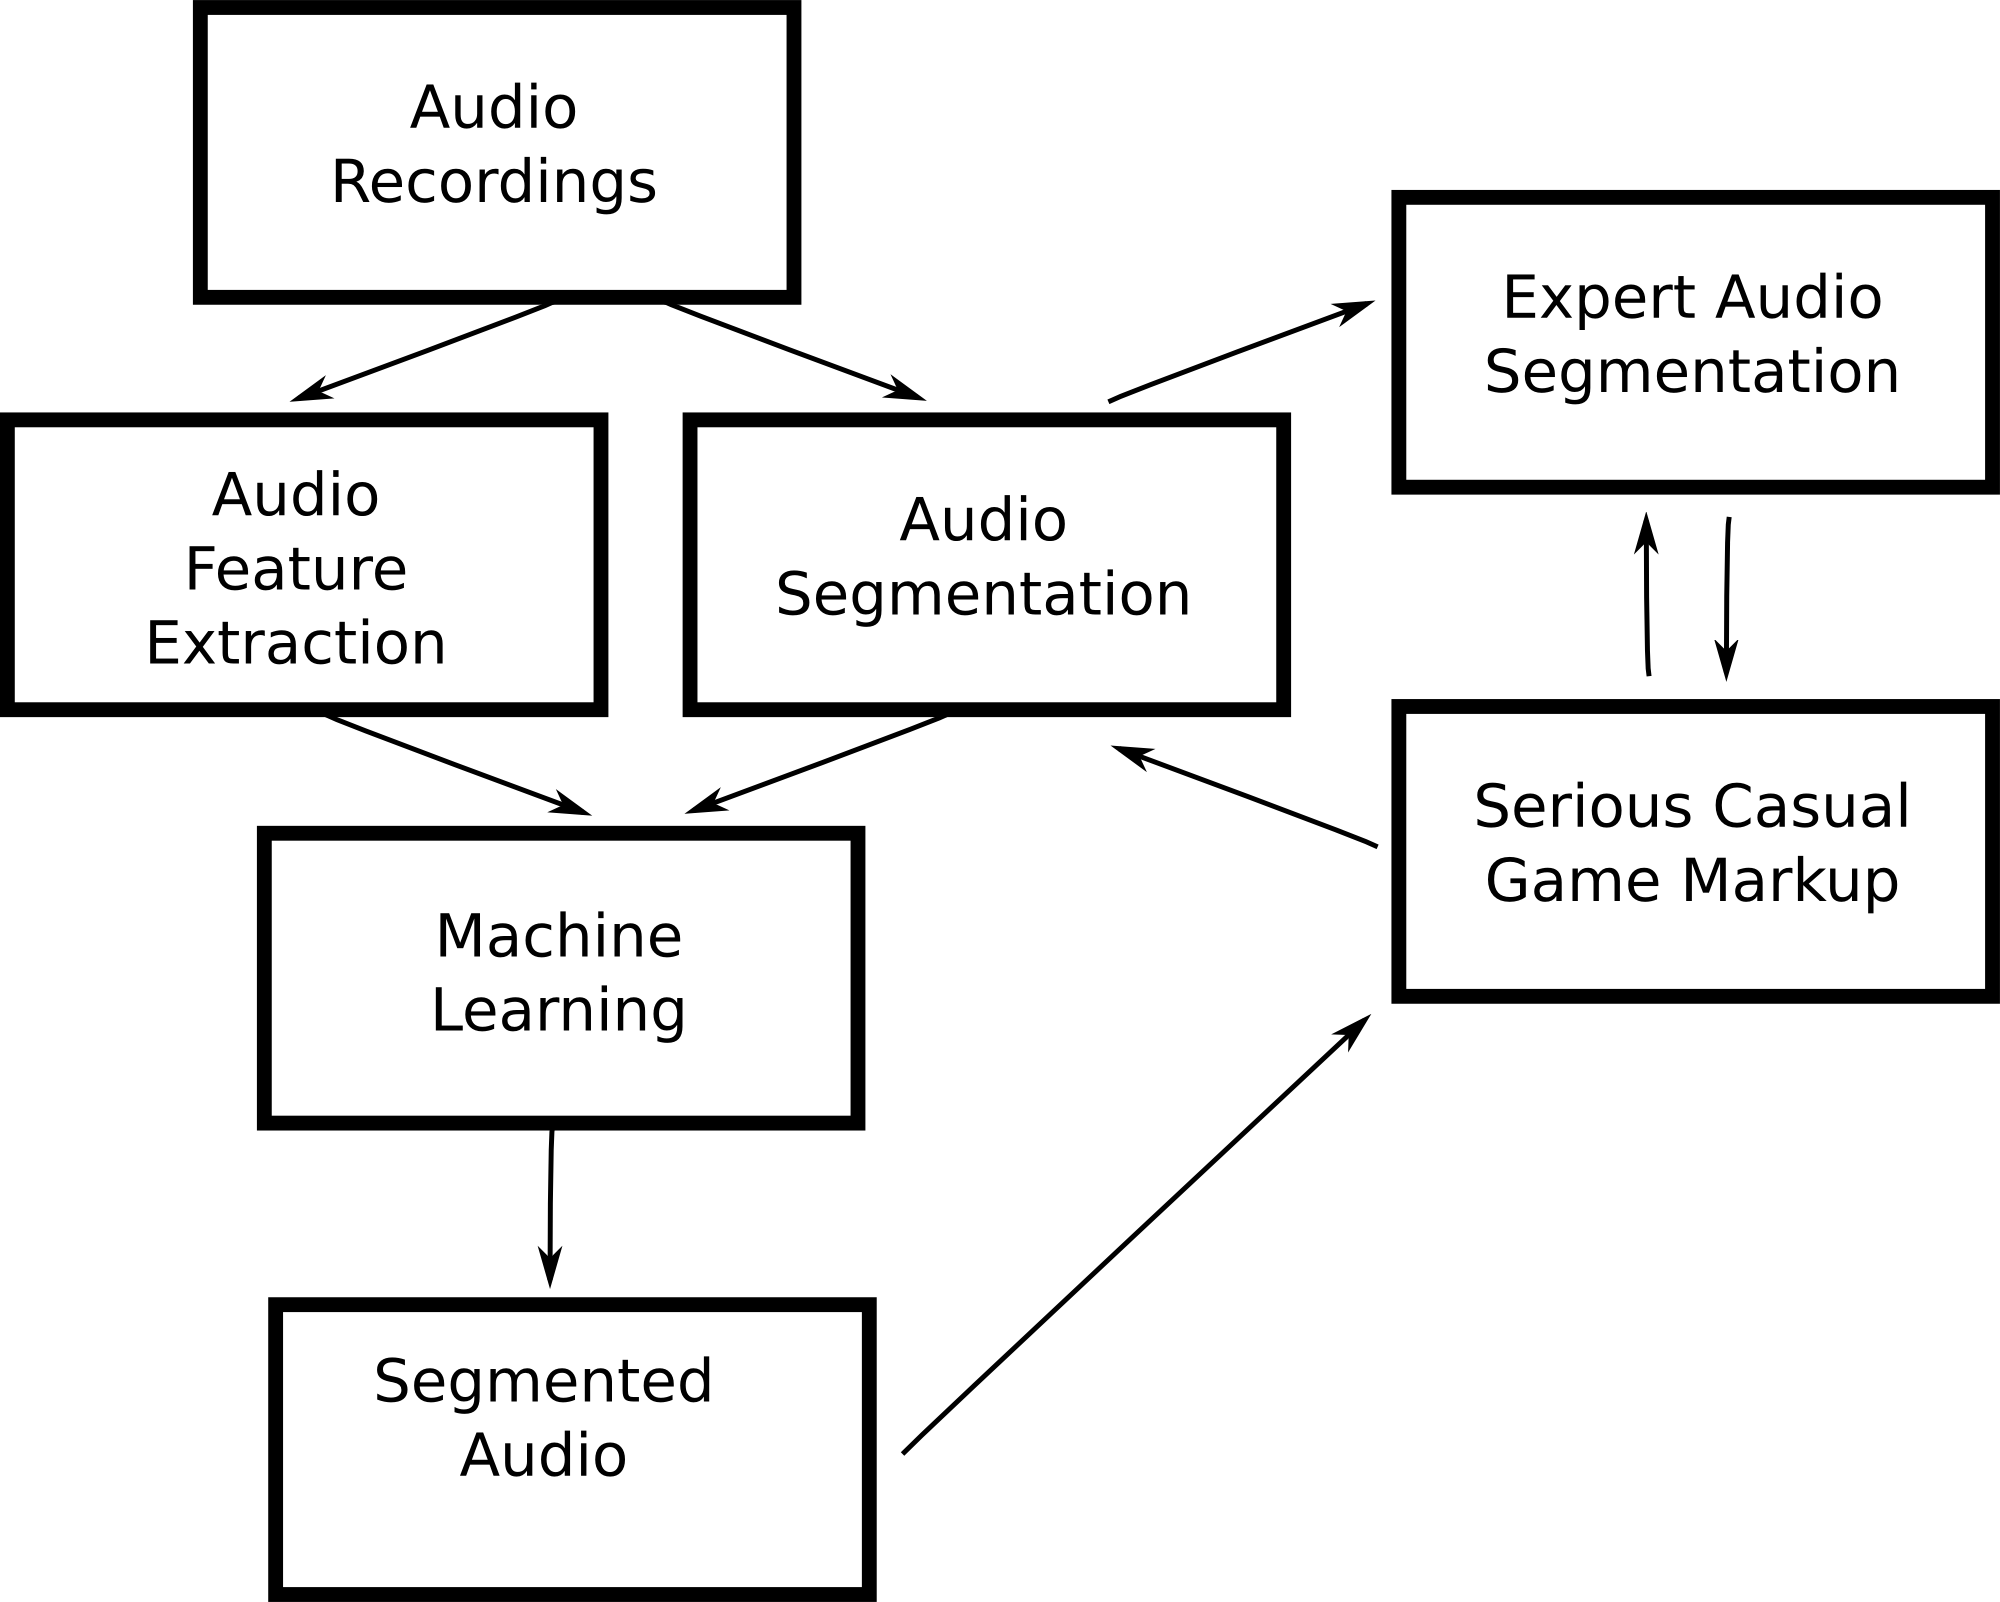
\includegraphics[width=80mm]{figures/systemDiagram}
\caption{System Diagram} 
\label{fig:systemDiagram} 
\end{figure} 

In order to do this, we will compare a number of different solutions
for doing distributed audio feature extraction and Machine Learning
and will compare not only their performance in classifying audio, but
also our experience with using these tools.

For my evaluation, we will generate two different types of results.
The first type will be the output of the audio feature extraction and
Machine Learning task. For this task, we will look at the distribution
of orca vocalizations in the dataset, and will train Machine Learning
classifiers that can distinguish regions of the Orchive that have
individual orca vocalizations.

In order to analyze the audio in large online archives efficiently, a
scenario involving distributed computing must be used.  There are many
different types of systems that perform Machine Learning and many of
these can distribute their work to different machines.  Some of these
systems are better suited for this task than others, and in this paper
we investigate a few combinations of these tools.

One of the possible solutions to the problem of the segmentation of
audio into orca vocalizations and other sounds is to use a Machine
Learning supervised classifier system.  These systems require hand
labelled training data, in our particular case, audio would be
labelled as either orca or background.  This training data is then
used to train a classifier system that can classify future instances
based on features of the training data.  There are a wide variety of
classification algorithms that are commonly used, some of the most
popular are Support Vector Machines (SVMs), Neural Nets, Decision
Trees and Logistic Regression.  In our past work we have found good
success in using SVMs, and have shown that SVMs typically outperform
many other Machine Learning algorithms.  However, there is current
work in this area showing the benefits of many alternate algorithms
for different problem domains.

There are two steps to the problem of the classification of audio
signals.  The first is that of audio feature extraction, and the
second is that of classification with Machine Learning systems.  Sound
is a pressure wave in the air, and the variations in pressure over
time can be stored in a computer as real number values.  This raw
waveform data contains all the information of the signal, but because
of it's extremely high dimensionality, is difficult to analyze with
machine learning systems.  To take this raw data and to put it in a
form more conducive for analysis, we generate a large number of higher
level features, including spectral features \cite{marsyas}, pitch
information \cite{cheveigne02}, chromatic scale information
\cite{marsyas} and other features based on models of the auditory
cortex \cite{lyon82}.  One can also model the statistical behaviour of
these properties as they change over time, an avenue that has been
shown to be fruitful \cite{marsyas}.  In our system we investigated
the use of a number of audio features, the results of which are
discussed in the Evaluation section, but in summary we found that
using all the standard audio features was most useful, however using
pitch information degraded performance of the classifier.  This is a
surprising result and one that we are investigating further.

The second step is to take these audio features, train and test a
Machine Learning classifer on them, and then run this Machine Learning
classifier over all the data.  In many cases it is beneficial to
pre-calculate the audio features for the data, as once as good
parameters can be determined for the audio feature extraction engine,
such as the window size, hop size for the spectrum calculation and the
memory size for the windowed statistical calculations, these features
can be saved and reused in multiple Machine Learning experiments with
different parameters.  One example of this is the recent release of
the Echonest audio features for the Million Song Dataset
\cite{bertinmahieux11}.  This collection of audio features for one
million popular songs took a considerable amount of time to process,
and one approach is to save these audio features and running different
machine learning algorithms or different parameter sets of these
algorithms on them.  Another point that should be made here is that
the form of the features that are extracted in this step can have a
direct relation to the performance of the subsequent Machine Learning
step.  Different algorithms perform better with different forms of
data, and matching the right features to the right algorithm is both
an art and a science.

It should be noted that both of these steps, the audio feature
extraction and the Machine Learning could be carried out in the same
executable.  There are a number of advantages to this as well as some
disadvantages.  One major advantage is that the intermediate audio
feature data does not have to be saved on disk.  This intermediate
data can be very large in size, and can be many times larger in size
than the original audio data, depending on the type of compression
used for the original audio.  In many cases in the real world, it is
less expensive to just recalculate the audio features each time that a
new Machine Learning run is carried out rather than saving them on
disk.  This also can help to overcome any versioning problems, where
different versions of audio features are combined together in the
training, testing or predicting stages.  It will be a balance between
these two poles for production systems to manage.

For this work, Marsyas was used for doing Audio Feature Extraction.
There are other Music Information Retrieval toolkits for extracting
audio features, but the audio features output by Marsyas are typically
amongst the most robust and high performing in the literature
\cite{marsyas}.  We have implemented this feature extraction using
native filesystem operations loading data off of NFS or a local disk
depending on the cluster situation.

For the Machine Learning half of the project, a variety of Machine
Learning systems and algorithms were used and comparison of them in is
provided in the evaluation section.  Results have been produced for a
Logistic Regression system using a Stochastic Gradient Descent
algorithm on Mahout, a distributed Machine Learning system implemented
as a Java library on top of Hadoop, an open source clone of the Google
File System (GFS) and Google MapReduce system.  These results are
compared to a Logistic Regression system using a quasi Newton solver
as implemented in Weka, a popular system for Machine Learning and show
timing and classification results of this system run as a grid style
parallel job on Westgrid.  These results for Logistic Regression are
then compared to three different implementations of a Support Vector
Machine (SVM) classifier.  The first of these is simply the SVM mode
in Weka but run in a grid-style distributed manner.  The second of
these is a parallel version of the SVM algorithm, PSVM
\cite{chang07psvm}.  The third of these is a hybrid audio feature
extraction and SVM developed in the Marsyas framework.  These three
different systems will be compared and contrasted in the Evaluation
section.

I propose to use the Westgrid system for running the huge audio
feature extraction task. This uses a very simple queuing system known
as Torque, which is the latest evolution of the ancient PBS (Parallel
Batch System) parallel job distribution system. PBS allows scientific
users to schedule large jobs to run on computers, and performs well
for certain scientific tasks where a single, usually large, program is
run on a variety of different datasets, and the results are then saved
to disk and later analyzed by a scientist. This type of computing was
traditionally known as Grid Computing.  While this system has certain
benefits for running specific scientific tasks, for other tasks, the
methodology of having separate computers running mostly independently,
and all coordination of tasks being the responsibility of the
programmer with an tool such as MPI quickly becomes difficult. The
MapReduce paradigm helps in the coordination of large parallel tasks,
and the Hadoop system allows programmers to efficiently write
distributed programs that run on huge numbers of computers and allows
for failures of individual computers. In this project we will use the
Mahout Machine Learning framework on top of a Hadoop installation to
process the audio feature vectors output by Marsyas and to gain
insights into the vocalization data in the Orchive. The primary task I
will investigate in this project will be identifying regions of the
Orchive with distinct orca vocalizations that are nearby to
hydrophones and isolated from other orca vocalizations.

Mahout is a Machine Learning framework that interacts closely with
Hadoop to both store the data and also run the Machine Learning
algorithms.  Hadoop is an open source port of the GFS
\cite{ghemawat03} and MapReduce \cite{dean08} infrastructure and
allows users to run large jobs that follow the map reduce paradigm.
In this scheme, a parallel job is split into two phases, a map phase
and a reduce phase.  In the map phase, key value pairs are generated
by some given algorithm from an input file, this same process occurs
in parallel on many other nodes, and the data that is used by a given
map is determined by the locality of data on that node.  These key
value pairs are then sorted and shuffled to a set of reduce nodes,
which take the collections of key value pairs and do an operation on
them that in some way combines, or reduces, the data.  These map and
reduce functions can be thought of as similar to the map and reduce
functions in functional programming, however, it should be noted that
this is a loose similarity due to the lack of higher order functions
in the current MapReduce implementation.  Many algorithms have been
ported to use this MapReduce type system, some of the most natural are
those that process large collections of text for building inverted
indexes or other tasks for searches, which is not surprising noting
the provenance of the MapReduce algorithm.  For other tasks, such as
those common in audio feature extraction, the reduce phase is simply
an identity reduce, where the map outputs are copied verbatim to the
reduce outputs.  It is easier and more natural to make some algorithms
more efficient in a MapReduce context than others.

The Mahout Machine Learning framework has implemented many different
Machine Learning algorithms in it's framework, including clustering,
recommendation and classification algorithms.  In our current work we
are more interested in classification than either recommendation or
clustering, and Mahout boasts support for the following classification
algorithms: Logistic Regression (SGD), Bayesian, Support Vector
Machines (SVM), Perceptron and Winnow, Neural Network, Random Forests,
Restricted Boltzmann Machines, Online Passive Aggressive, Boosting and
Hidden Markov Models.  However, after investigation, it appears most
of these algorithms are in a definite alpha state, and require
patching of the main source tree with external files.  The two most
well supported classification algorithms in Mahout are the Logistic
Regression classifier, using a Stochastic Gradient Descent (SGD)
engine, and a Naive Bayesian classifier.  Upon extensive
investigation, the Bayesian classifier makes many internal assumptions
of the input being of large bodies of written text and was not
suitable for our use case.  However, the Logistic Regression
classifier was well suited to our data and performed well in our
tests.

One advantage of using the Mahout Machine Learning framework was that
it stored its input and output data on HDFS, the Hadoop Distributed
Filesystem.  When working with the huge amounts of data that are
generated by audio feature extraction and Machine Learning
experiments, managing and transferring experimental results from the
grid servers to the production web servers is often a time consuming
and error prone procedure.  After our experience with Hadoop, we have
integrated it into web application and use the WebHDFS system to serve
all experimental results to users.  These users interact with a web
application that displays some data obtained from the production web
server but also displays the results of experiments as data served
live from a WebHDFS system that is being populated by the experimental
results from live requests from scientists.


\section{Web based interfaces}


- Expert Interface
- Citizen Science Interface
- Old interface
	- Static resources
	- Difficult to regenerate
	- Many different technologies
		- RoR, HaXe, Flash, Javascript, Python, C++
	- Files generated by hand and manually added to server
	- Many different websites with different technology


- New interface
	- Fewer technologies
		- Javascript (client+server), Python, C++
	- Unified interface to all technologies
	- Interfaces to many programs




\section{Audio Feature Extraction}


- MFCC


- Pitch


- Side Band Intervals


- Stabilized Auditory Image


- Bioinformatic algorithms


\section{Auditory Sparse Coding}

The concept of sparsity has attracted considerable interest in the
field of machine learning in the past few years.  Sparse feature
vectors contain mostly values of zero and one or a few non-zero
values.  Although these feature vectors can be classified by
traditional machine learning algorithms, such as SVM, there are
various recently-developed algorithms that explicitly take advantage
of the sparse nature of the data, leading to massive speedups in time,
as well as improved performance.  Some fields that have benefited from
the use of sparse algorithms are finance, bioinformatics, text mining
\cite{balakrishnan2008}, and image classification \cite{chechik2010}.
Because of their speed, these algorithms perform well on very large
collections of data \cite{bottou2007}; large collections are becoming
increasingly relevant given the huge amounts of data collected and
warehoused by Internet businesses.

In this chapter, we discuss the application of sparse feature vectors
in the field of audio analysis, and specifically their use in conjunction with 
preprocessing systems that model the human auditory system. We present early
results that demonstrate the applicability of the combination of 
auditory-based processing and sparse coding to content-based audio analysis 
tasks.

Traditional approaches to audio analysis problems typically employ a 
short-window fast Fourier transform (FFT) as the first stage of the processing 
pipeline. In such systems a short, perhaps 25ms, segment of audio is taken 
from the input signal and windowed in some way, then the FFT of that segment 
is taken. The window is then shifted a little, by perhaps 10ms, and the 
process is repeated. This technique yields a two-dimensional spectrogram of 
the original audio, with the frequency axis of the FFT as one dimension, and 
time (quantized by the step-size of the window) as the other dimension.

While the spectrogram is easy to compute, and a standard engineering
tool, it bears little resemblance to the early stages of the
processing pipeline in the human auditory system. The mammalian
cochlea can be viewed as a bank of tuned filters the output of which
is a set of band-pass filtered versions of the input signal that are
continuous in time. Because of this property, fine-timing information
is preserved in the output of cochlea, whereas in the spectrogram
described above, there is no fine-timing information available below
the 10ms hop-size of the windowing function.

This fine-timing information from the cochlea can be made use of in
later stages of processing to yield a three-dimensional representation
of audio, the stabilized auditory image (SAI)\cite{patterson2000},
which is a movie-like representation of sound which has a dimension of
`time-interval' in addition to the standard dimensions of time and
frequency in the spectrogram. The periodicity of the waveform gives
rise to a vertical banding structure in this time interval dimension,
which provides information about the sound which is complementary to
that available in the frequency dimension. A single example frame of a
stabilized auditory image is shown in Figure~\ref{fig:sai}.

While we believe that such a representation should be useful for audio
analysis tasks, it does come at a cost. The data rate of the SAI is
many times that of the original input audio, and as such some form of
dimensionality reduction is required in order to create features at a
suitable data rate for use in a recognition system. One approach to
this problem is to move from a the dense representation of the SAI to
a sparse representation, in which the overall dimensionality of the
features is high, but only a limit number of the dimensions are
nonzero at any time.

In recent years, machine learning algorithms that utilize the
properties of sparsity have begun to attract more attention and have
been shown to outperform approaches that use dense feature vectors.
One such algorithm is the passive-aggressive model for image retrieval
(PAMIR), a machine learning algorithm that learns a ranking function
from the input data, that is, it takes an input set of documents and
orders them based on their relevance to a query. PAMIR was originally
developed as a machine vision method and has demonstrated excellent
results in this field.

There is also growing evidence that in the human nervous system
sensory inputs are coded in a sparse manner; that is, only small
numbers of neurons are active at a given time \cite{olshausen2004}.
Therefore, when modeling the human auditory system, it may be
advantageous to investigate this property of sparseness in relation to
the mappings that are being developed. The nervous systems of animals
have evolved over millions of years to be highly efficient in terms of
energy consumption and computation.  Looking into the way sound
signals are handled by the auditory system could give us insights into
how to make our algorithms more efficient and better model the human
auditory system.

One advantage of using sparse vectors is that such coding allows very
fast computation of similarity, with a trainable similarity measure
\cite{chechik2010}. The efficiency results from storing, accessing,
and doing arithmetic operations on only the non-zero elements of the
vectors.  In one study that examined the performance of sparse
representations in the field of natural language processing, a 20- to
80-fold speedup over LIBSVM was found \cite{haffner2006}.  They
comment that kernel-based methods, like SVM, scale quadratically with
the number of training examples and discuss how sparsity can allow
algorithms to scale linearly based on the number of training examples.

In this chapter, we use the stabilized auditory image (SAI) as the
basis of a sparse feature representation which is then tested in a
sound ranking task and a music information retrieval task. In the
sound raking task, we generate a two-dimensional SAI for each time
slice, and then sparse-code those images as input to PAMIR.  We use
the ability of PAMIR to learn representations of sparse data in order
to learn a model which maps text terms to audio features.  This PAMIR
model can then be used rank a list of unlabeled sound effects
according to their relevance to some text query. We present results
that show that in certain tasks our methods can outperform highly
tuned FFT based approaches. We also use similar sparse-coded SAI
features as input to a music genre classification system. This system
uses an SVM classifier on the sparse features, and learns text terms
associated with music. The system was entered into the annual music
information retrieval evaluation exchange evaluation (MIREX 2010).

Results from the sound-effects ranking task show that sparse
auditory-model-based features outperform standard MFCC features,
reaching precision about 73\% for the top-ranked sound, compared to
about 60\% for standard MFCC and 67\% for the best MFCC variant.
These experiments involved ranking sounds in response to text queries
through a scalable online machine learning approach to ranking.

In our system we have taken inspiration from the human auditory system
in order to come up with a rich set of audio features that are
intended to more closely model the audio features that we use to
listen and process music.  

Such fine timing relations are discarded by traditional spectral
techniques.  A motivation for using auditory models is that the
auditory system is very effective at identifying many sounds.  This
capability may be partially attributed to acoustic features that are
extracted at the early stages of auditory processing.  We feel that
there is a need to develop a representation of sounds that captures
the full range of auditory features that humans and animals use to
discriminate and identify different sounds, so that machines have a
chance to do so as well.

This SAI representation generates a 2D image from each section of
waveform from an audio file.  We then reduce each image in several
steps: first cutting the image into overlapping boxes converted to
fixed resolution per box; second, finding row and column sums of these
boxes and concatenating those into a vector; and finally vector
quantizing the resulting medium-dimensionality vector, using a
separate codebook for each box position.  The VQ codeword index is a
representation of a 1-of-N sparse code for each box, and the
concatenation of all of those sparse vectors, for all the box
positions, makes the sparse code for the SAI image.  The resulting
sparse code is accumulated across the audio file, and this histogram
(count of number of occurrences of each codeword) is then used as
input to an SVM \cite{yh05} classifier\cite{chapelle2006}.  This
approach is similar to that of the ``bag of words'' concept,
originally from natural language processing, but used heavily in
computer vision applications as ``bag of visual words''; here we have
a ``bag of auditory words'', each ``word'' being an abstract feature
corresponding to a VQ codeword.  The bag representation is a list of
occurrence counts, usually sparse.


\section{Algorithm}

In our experiments, we generate a stream of SAIs using a series of modules
that process an incoming audio stream through the various stages of the 
auditory model. The first module filters the audio using the
pole--zero filter cascade (PZFC) \cite{lyon10}, then subsequent modules find 
strobe points in this audio, and generate a stream of SAIs at a rate of 50 per 
second. The SAIs are then cut into boxes and are transformed into a high 
dimensional dense feature vector \cite{rehn2009} which is vector quantized to 
give a high dimensional sparse feature vector. This sparse vector is then used 
as input to a machine learning system which performs either ranking or 
classification. This whole process is shown in diagrammatic form in Figure 
~\ref{fig:flowchart}

We first process the audio with the pole--zero filter cascade (PZFC)
\cite{lyon10}, a model inspired by the dynamics of the human
cochlea. The PZFC is a cascade of a large number of simple filters
with an output tap after each stage. The effect of this filter cascade
is to transform an incoming audio signal into a set of band-pass
filtered versions of the signal. In our case we used a cascade with 95
stages, leading to 95 output channels. Each output channel is
half-wave rectified to simulate the output of the inner hair cells
along the length of the cochlea. The PZFC also includes an automatic
gain control (AGC) system that mimics the effect of the dynamic
compression mechanisms seen in the cochlea. A smoothing network, fed
from the output of each channel, dynamically modifies the
characteristics of the individual filter stages. The AGC can respond
to changes in the output on the timescale of milliseconds, leading to
very fast-acting compression. One way of viewing this filter cascade
is that its outputs are an approximation of the instantaneous neuronal
firing rate as a function of cochlear place, modeling both the
frequency filtering and the automatic gain control characteristics of
the human cochlea \cite{lyon1990}. The PZFC parameters used for the
sound-effects ranking task are described in \cite{lyon10}. We did not
do any further tuning of this system to the problems of genre, mood or
song classification; this would be a fruitful area of further
research.

\subsection{Image Stabilization}

The output of the PZFC filterbank is then subjected to a process of
strobe finding where large peaks in the PZFC signal are found.  The
temporal locations of these peaks are then used to initiate a process
of temporal integration whereby the stabilized auditory image is
generated.  These strobe points ``stabilize'' the signal in a manner
analogous to the trigger mechanism in an oscilloscope.  When these
strobe points are found, a modified form of autocorrelation, known as
strobed temporal integration, which is like a sparse version of
autocorrelation where only the strobe points are correlated against
the signal. Strobed temporal integration has the advantage of being
considerably less computationally expensive than full autocorrelation.

\subsection{Box Cutting}

We then divide each image into a number of overlapping boxes using the
same process described in \cite{lyon10}.  We start with rectangles of
size 16 lags by 32 frequency channels, and cover the SAI with these
rectangles, with overlap.  Each of these rectangles is added to the
set of rectangles to be used for vector quantization.  We then
successively double the height of the rectangle up to the largest size
that fits in an SAI frame, but always reducing the contents of each
box back to 16 by 32 values.  Each of these doublings is added to the
set of rectangles.  We then double the width of each rectangle up to
the width of the SAI frame and add these rectangles to the SAI frame.
The output of this step is a set of 44 overlapping rectangles. The
process of box-cutting is shown in Figure ~\ref{fig:boxcutting}. In
order to reduce the dimensionality of these rectangles, we then take
their row and column marginals and join them together into a single
vector.

The resulting dense vectors from all the boxes of a frame are then
converted to a sparse representation by vector quantization.

\subsection{Campana}

In the paper ``Monitoring and Mining Insect Sounds in Visual
Space''\cite{hao12}, Hao et al. describe a novel method for data
mining large databases of insect sounds.  Their method is completely
automated, and does not require human experts to label data, as is the
case in most other systems of this type.  They perform classification
of sounds based on the spectrogram, a visual representation of a sound
that gives a frequency versus time plot of a sound.  They use a recent
distance measure called the Campana-Keogh (CK) measure to compare the
textures of two images.

The paper first describes the importance of monitoring and measuring
of the sounds of animals and insects.  In the natural habitat, the
sounds of animals can be used to determine how many animals are in a
location and what species these animals are, and can help scientists
measure the biodiversity of a location, and how this biodiversity
changes over time.  There is recent interest in this field of study
\cite{wimmer2010} \cite{seuer2008} as a method for determining the
biodiversity changes in regions over time.  The authors then say that
an automated system for detecting insects would also be useful from a
commercial point of view,

The paper then goes on to say that in laboratory settings, it would
also be advantageous to have an automated system that could segment
and classify recordings.  Currently this task often requires
researchers to annotate hundreds of recordings by hand, which is a
very time intensive task.  As a scientist who has done many hours of
hand annotating of large sound archives, I can attest to the
difficulty and time-consuming nature of this task.

The authors then say that there are many problems with current methods
of detecting, segmenting and classifying the sounds and vocalizations
of animals.  Current methods require researchers to manually annotate
recordings and to generate a large corpus of data to be used by
classification algorithms.  These algorithms often have a large number
of tunable parameters, some of which can be automatically determined
from the large amount of training data, and some which have to be
manually explored by the researchers.  In addition, many of these
algorithms are computationally expensive and cannot be deployed in the
field.  I have found these facts to be true in my own research, and I
appreciate the fact that the authors spend time discussing the
problems faced by researchers studying bioacoustics.

In this section, they first define a sound sequence as a continuous
sequence of real valued data.  They then go on to define a spectrogram
as a visual spectral representation of an acoustic signal.  They
define a sliding window as a local subsection of a sound sequence, and
define a subsequence and a way to measure distances between
subsequences.

They then move on to more interesting definitions, first of the
entropy of a sound sequence dataset:
	\[ E(D) = -p(X)log(p(X)) - p(Y)log(p(Y)) \]

The information gain for a given splitting strategy is then defined as
	\[ Gain = E(D) - E'(D) \]

Where $E(D)$ and $E'(D)$ are the entropy before and after $D$ is
partitioned into $D_1$ and $D_2$.

	\[ E(D) = f(D_1)E(D_1) + f(D_2)E(D_2) \] 

Where $f(D_1)$ and $f(D_2)$ are the fraction of the objects that are
in $D_1$ and $D_2$, respectively.

They then point out that given a linear ordering of annotated objects
in $D$, there exist at most $|D|-1$ distinct splitting points that
divide the ordered objects into two distinct sets.  Finally, they
define a sound fingerprint for a species as the subsequence from P
along with its best splitting point that produces the largest
information gain when compared with the non-matching sequences U.

They then go on to provide an figure that explains in rough detail
what their distance measure looks like.  This is shown here in Figure
\ref{fig:campana_figure2}.  I found these examples to be unclear at
first, but on deep examination and by staring at it for quite some
time, I figured out what they were trying to say.  In these examples,
they show some sound fingerprints with arrows pointing to a line below
them.

They first describe the Brute-Force algorithm, which basically just
searches over all possible combinations of subsequences for P and U,
and computes the distance between all these subsequences.  The
equation for this is:

\[ \sum^{L_{max}}_{l=L_{min}} \sum_{S_i \in { P }} (M_i - l + 1) \]

While this algorithm guarantees that the best subsequence will be
found, it is quite expensive in terms of computer time, and even for
their toy dataset of 10 sound files of the insect they are looking for
and 10 sound files of other sounds, would take 1,377,800 calls to the
CK distance measure, which is the most time intensive part of the
whole process.

To reduce the computation time, they first investigate Admissible
Entropy Pruning, in which they note that they can easily compute the
upper bound of an ordering, and if this upper bound is less than the
best-so-far information gain of any previously determined ordering,
they can abandon the current search and move on to the next candidate.
For their toy problem, this only reduces the total number of
comparisons, but in a data mining context, where huge databases are
searched, they say this could prune the total number of calculations
by 95\%.  This Entropy Pruning algorithm is one of the key insights of
this paper.  Without it, their CK distance measure would likely be too
expensive to use on real datasets, and by using Entropy Pruning, they
are able to speed up their algorithm by a large factor.

The method that this paper proposes is to classify animal sounds in
the visual space by examining the texture of the spectrogram of the
sounds, and finding the smallest acoustic fingerprint that is
representative of the species.  The texture of an image is a concept
commonly used in the field of image processing and describes the
quantitative relationship of light and dark patterns in an image.

The images that this paper proposes to examine are spectrograms of an
audio file.  A spectrogram shows the time-frequency evolution of a
sound, commonly calculated by a Fast Fourier Transform (FFT).  There
is a long tradition involving the manual inspection of spectrograms to
analyse the vocalizations of organisms, one among many of these is the
Orca call catalog from Ford \cite{ford87}.  In these approaches, a
human manually inspects and classifies spectrograms.

I found that this is an interesting and novel way of approaching the
problem of classifying and annotating the sounds made by organisms.
Most other approaches use single time slices of spectral data, which
are sometimes averaged over time.  The idea of looking at sounds in
the visual space in fact means that instead of looking at a single
time point, the time evolution of sounds is instead investigated.
While in the sub-field of symbolic Music Information Retrieval (MIR),
there has been some research into the time structure of sound, in most
audio-based approaches to MIR, the time evolution of music is
explicitly ignored.  This is likely because this would dramatically
complicate the analysis of sound, and in most of the problems that
have been investigated by researchers, such as genre detection in
songs, this additional complexity does not significantly improve
results.  However, when looking at bioacoustics, the time evolution of
signals can be very important.

There are many methods in the literature for computing the similarity
of two images by their textures that they have.  Some of these include
wavelets, Fourier transforms and Gabor filters.  The authors describe
one problem of these methods is that they often have many tunable
parameters, and that the exact values of these parameters can have
considerable impact on their classification performance.

In this paper they use a previously described distance measure called
the Campana-Keogh (CK) measure \cite{campana2010} which uses the
concept that two images are similar if one image can be used to
compress the other image.  The CK measure uses the MPEG-1 algorithm to
calculate the distance between two images and its formula is shown
below:

	\[ dist = \frac{mpegSize(x,y) + mpegSize(y,x)} {mpegSize(x,x) + mpegSize(y,y)} - 1 \]

This surprisingly simple measure has been shown to work well in a
variety of contexts, including the comparison of images of moths, wood
grains, nematodes and tire tracks\cite{campana2010}.

I find this part of the paper to be very interesting and novel.  On
first reading, I found it difficult to belive that such a simple
scheme would work, but on further reflection, the idea that two sounds
are similar if one can be used to compress the other could be an
excellent approach to the study of these signals.

They first describe the Brute-Force algorithm, which basically just
searches over all possible combinations of subsequences for P and U,
and computes the distance between all these subsequences.  The
equation for this is:

	\[ \sum^{L_{max}}_{l=L_{min}} \sum_{S_i \in { P }} (M_i - l + 1) \]

To reduce the computation time, they first investigate Admissible
Entropy Pruning, in which they note that they can easily compute the
upper bound of an ordering, and if this upper bound is less than the
best-so-far information gain of any previously determined ordering,
they can abandon the current search and move on to the next candidate.
For their toy problem, this only reduces the total number of
comparisons, but in a data mining context, where huge databases are
searched, they say this could prune the total number of calculations
by 95\%.  This Entropy Pruning algorithm is one of the key insights of
this paper.  Without it, their CK distance measure would likely be too
expensive to use on real datasets, and by using Entropy Pruning, they
are able to speed up their algorithm by a large factor.

They then further investigate ways to speed up their algorithm by
introducing a proxy for the CK distance measure using euclidean
distances.  They note that their algorithm orders candidate solutions,
and that the entropy pruning algorithm can eliminate poor solutions if
their upper information gain bound is less than the current best
solution.  They then go on to say that if they could generate better
solutions early in the search process, they could quickly eliminate
unpromising solutions.  This is however as they note, a
chicken-and-egg problem, as they cannot know what are these better
solutions before they find them.  In order to overcome this, they
introduce a Euclidean distance measure, and show via a graph that the
Euclidean distance is a good proxy for the CK distance, and is much
less expensive to compute.


\subsection{SAI}

In our system we have taken inspiration from the human auditory system
in order to come up with a rich set of audio features that are
intended to more closely model the audio features that we use to
listen and process music.  To this end we use the Stabilized Auditory
Image (SAI) \cite{lyon1990} \cite{patterson2000}, which combines
several different concepts, some of which directly model auditory
physiology and psychoacoustics, and some which are based more on a
general model of human auditory perception.  A single example frame of
a Stabilized Auditory Image is shown in Figure ~\ref{fig:sai}

\begin{figure}[here]
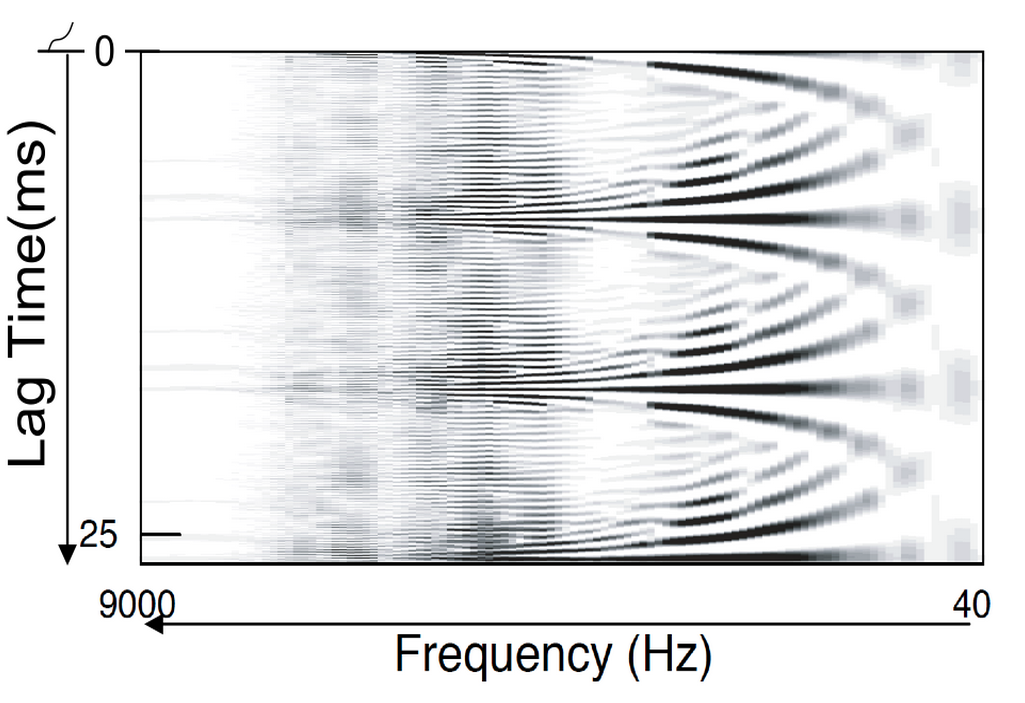
\includegraphics[width=150mm]{figures/sai}
\caption{Stabilized Auditory Image \label{fig:sai}}
\end{figure}

This SAI image representation generates a 2D image of each section of
samples from an audio file.  We then reduce this large amount of
information in two steps, first by cutting the image into overlapping
boxes and finding row and column residuals of these boxes, and then by
vector quantizing the resulting high dimensionality vector.  The
resulting spare vector is then histogrammed across the audio file, and
this histogram is then used as input to an SVM \cite{yh05}
classifier\cite{chapelle2006}.

The field of Music Information Retrieval (MIR) or Machine Hearing
\cite{marsyas} attempts to teach computers to understand music.  There
are a wide variety of tasks in this field that range from music
playlisting to analyzing Gregorian chants and Bach fugues.  Both in my
group at UVIC and at Google, we are specifically interested in
approaches that take audio as input.  From this audio we calculate a
variety of features, including the low, medium and high frequency
content and how these frequencies evolve over time.  We then use
advanced machine learning algorithms including Support Vector Machines
and Deep Belief Networks \cite{bengio2007}.

Most current approaches in MIR use spectral based approaches that use
the Fast Fourier Algorithm to decompose a signal into a set of
sinusoid's with a specific frequency and phase.  An example
spectrogram of a human voice is shown in Figure \ref{fig:spectrogram}.
These approaches are computationally efficient and fast, and give us a
good understanding of many features of music.  Using these features,
the field of MIR has had many successes, in the field of genre
recognition, for example, we often can achieve a classification
accuracy of 80\%.  In the past 5 years, most of the advances in MIR
have come from applying more and more advanced machine learning
algorithms to this problem.  It now appears that we have reached a
plateau where the performance of these systems is not increasing, and
it is felt that by using better audio features, performance can be
again improved.

FFT based approaches are fundamentally different from how our ear
actually hears sound.  FFT approaches take a window of data and
decompose this window into different sinusoids with a period and
phase.  The choice of window size involves a tradeoff between time
resolution and frequency resolution, and in order to increase time
resolution, frequency resolution must be decreased.  For certain
sounds produced in music, like those of sustained notes, this model
works well, but for many others, such as drum hits or the pulse
resonance phenomenon found in human voices, this model has
limitations.

The models of the human auditory system (Figure \ref{fig:humanear}
developed both by Dick Lyon \cite{slaney93} and other researchers
around the world have a fundamentally different approach in which
audio is filtered by a filterbank cascade that models features of the
human cochlea, the outputs of these filters are then processed by a
mechanism that is modeled on higher levels in the auditory periphery
that take this filterbank audio and generate two dimensional movie
frames that contain both frequency and an autocorrelation axis.  These
frames contain the fine timing information that is utilized by the
human hearing system to separate, localize and identify sounds.

This model finds trigger points in the input audio signal and
stabilizes the train of peaks from the CARFAC filterbank cascade into
a two dimensional image.  The output of the CARFAC filterbank is shown
in Figure \ref{fig:nap}, in this figure, the vertical axis corresponds
to cochlear place, with points closer to the bottom axis corresponding
to lower frequencies and the horizontal axis corresponding to time.
This plot can also be referred to as a Neural Activity Profile (NAP).
These peaks flow by rapidly, at the rate of pulses from the organism
in question, and in order to view them, one should align subsequent
peaks to each other.  There are many approaches to doing this, and the
approach commonly used is to find trigger points in the audio, that
is, points that correspond to pulses in the output of the vocal tract.
One trigger detection algorithm is shown schematically in Figure
\ref{fig:triggerpoints}.  In this figure the solid black line in the
center corresponds to the audio signal, and the red dots signify
trigger points.  The solid black line at the top of the figure
represents the current threshold value of the algorithm, and when this
threshold crosses the line representing the audio, a new trigger point
is generated.

In this section, we focus on retrieval rather than classification and
only use the ground truth labels as a way to measure retrieval
effectiveness. We compare different strategies over a large dataset
(185 calls, 4 classes) using well established retrieval effectiveness
measures. To the best of our knowledge this is the first systematic
evaluation of these different design choices.

\subsection{PZFC and CARFAC}
The CARFAC model includes a more advanced treatment of the fast acting
compression that the Outer Hair Cells in the cochlea perform to allow
the ear to hear both very loud and very soft sounds, a technique
formally referred to as Automatic Gain Control (AGC).  This model is
more advanced than the PZFC model, and this additional complexity can
be seen in Figure \ref{fig:dspcarfac}.

\begin{figure}[t]
\begin{center}
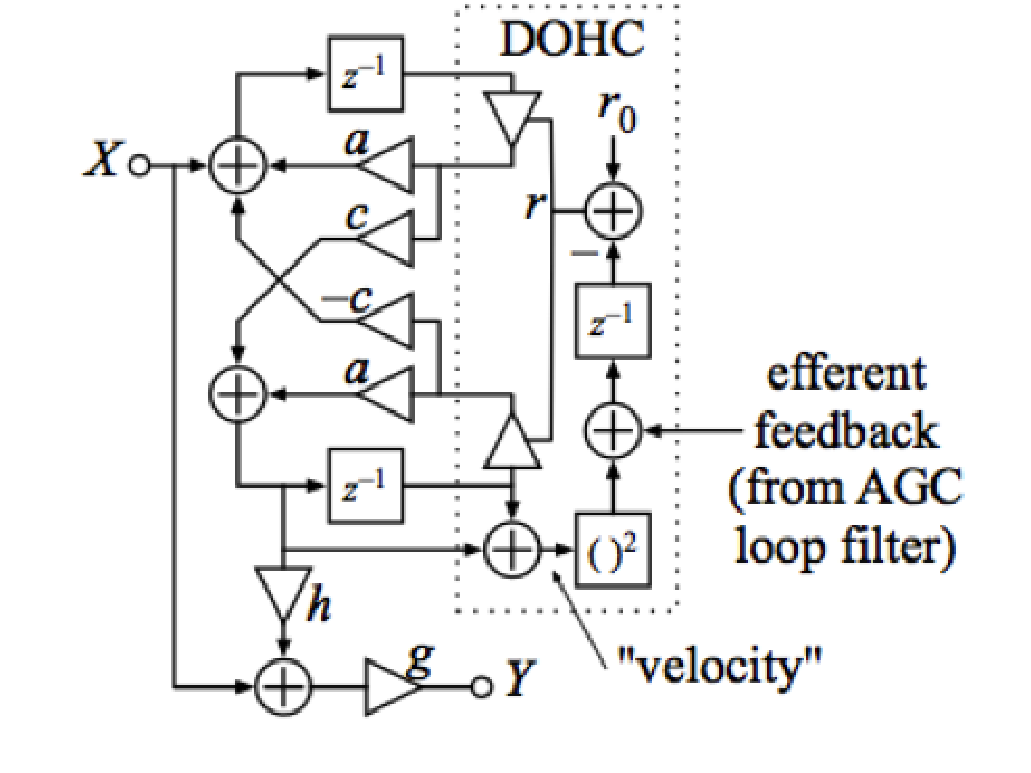
\includegraphics[width=50mm]{figures/dspcarfac}
\caption{
The Cascade of Asymmetric Filters and Resonators (CARFAC) model.  This
model is similar to the PZFC model, but includes an Automatic Gain
Control (AGC) stage, that models the action of the Outer Hair Cells in
the human cochlea.} 
\label{fig:dspcarfac} 
\end{center} 
\end{figure} 


The code for the CARFAC model was written in MATLAB, and it was my
task to take this code, port it to C++, verify that it worked
identically to the original code and then to optimize it to run as
quickly as possible.  For this, I used a software development
methodology called Test Driven Development \cite{fraser03} (TDD).  In
TDD, one inverts the normal software development process in that one
first writes the tests, and then the minimum code to make these tests
pass.  This is an ideal development strategy to use in this case,
since we have a working reference implementation of the algorithm in
MATLAB.  Using this strategy, I was able to port this MATLAB code
first to Python and then to C++.  The C++ code was added to the
Marsyas \cite{marsyas} framework and was open-sourced during my time
at Google, and is now available to be used by the community.

The process of porting the CARFAC model was straightforward but time
consuming.  After I had ported this model to C++, we then went back to
MATLAB to develop a model of binaural hearing using the output of the
CARFAC filter cascade.  We used the Stabilized Auditory Image (SAI) model
proposed by Patterson \cite{patterson92}, which works well for the
pulse resonance sounds created by many types of animals, from fish to
insects to the human voice.  In Figure \ref{fig:pulseresonance} the
sounds from various animals are shown, an in each one, the same
phenomenon is seen, where a fast impulse, or pulse is created and is
then resonated through the vocal tract or other sound producing organ
in the creature.

\begin{figure}[t]
\begin{center}
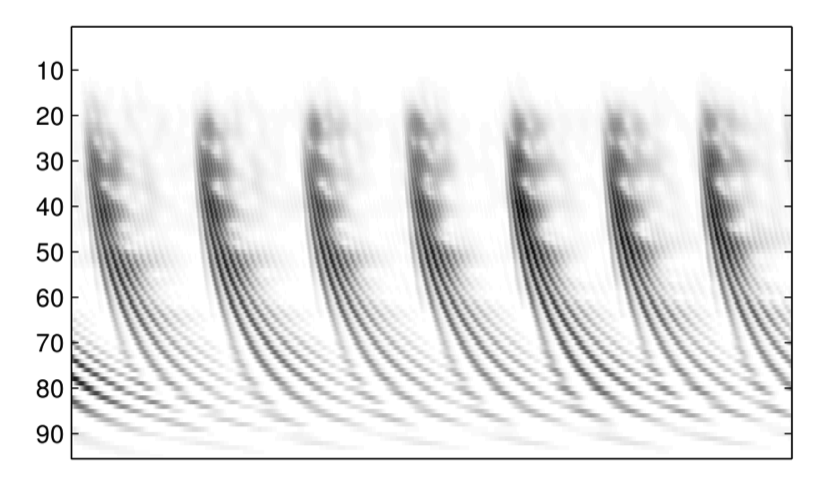
\includegraphics[width=100mm]{figures/nap}
\caption{ The Neural Activity Pattern (NAP) of the CARFAC model.  In
  this figure, the vertical axis corresponds to cochlear place, with
  points closer to the bottom axis corresponding to lower frequencies
  and the horizontal axis corresponding to time}
\label{fig:nap} 
\end{center} 
\end{figure} 

\begin{figure}[t]
\begin{center}
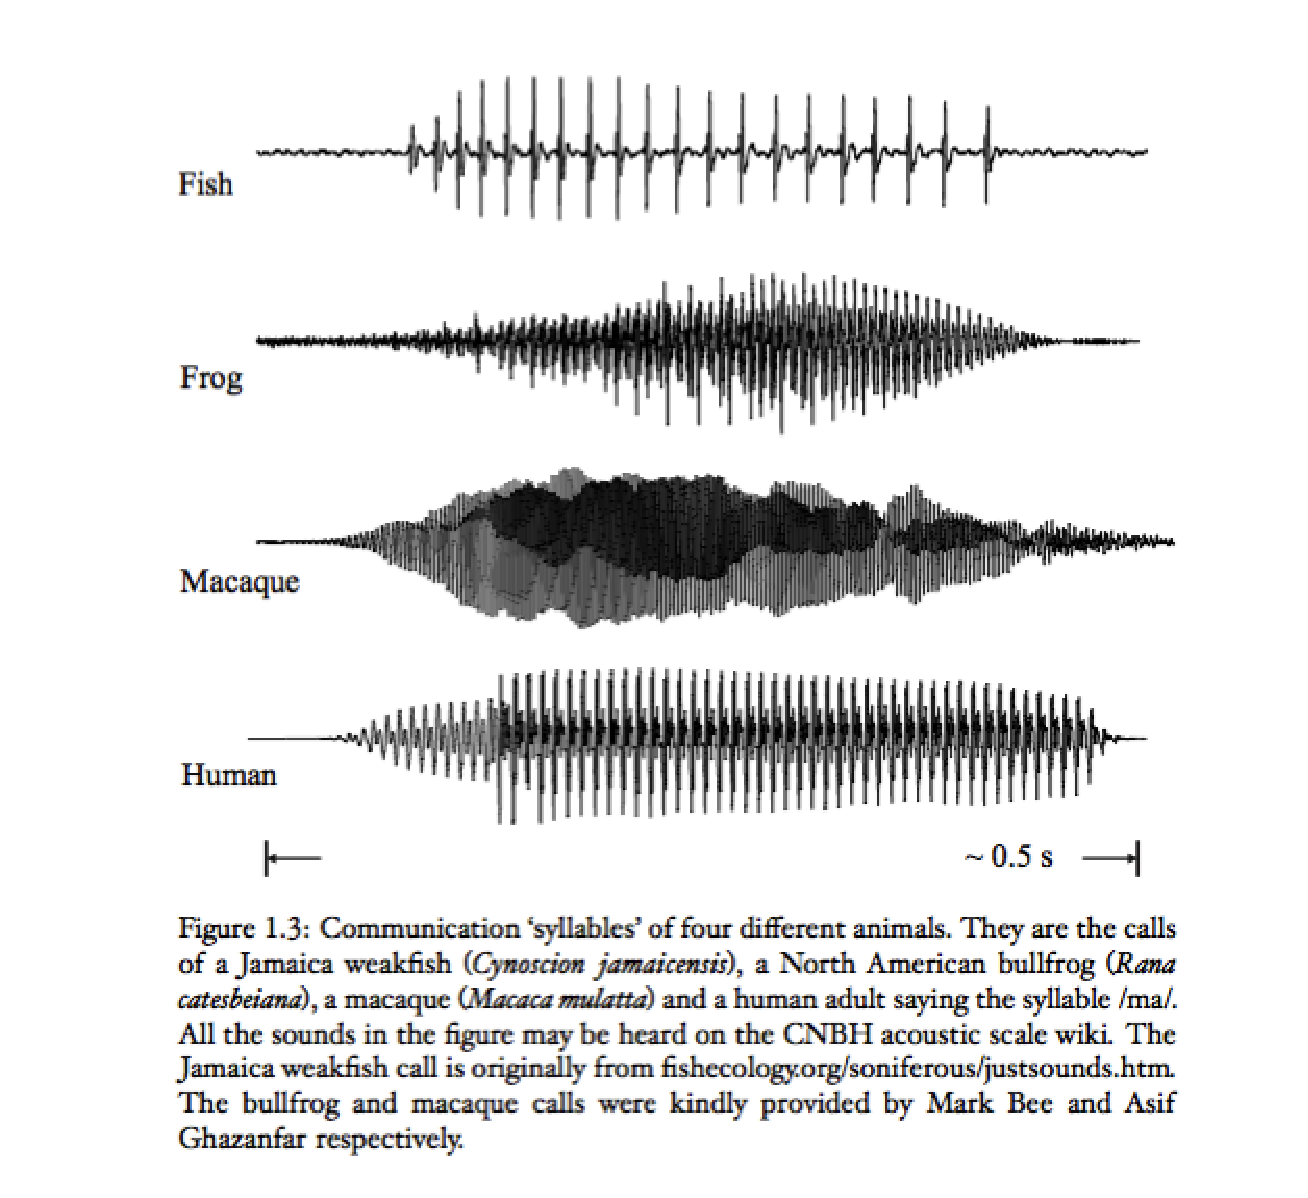
\includegraphics[width=100mm]{figures/pulseresonance}
\caption{ A diagram of the waveforms produced by a variety of
  different animals, showing the pulse and resonance structure of
  these vocalizations.  In each, a short pulse is generated which then
  reverberates through the vocal tract or sound producing organ of the
  organism.}
\label{fig:pulseresonance} 
\end{center} 
\end{figure} 

This model finds trigger points in the input audio signal and
stabilizes the train of peaks from the CARFAC filterbank cascade into
a two dimensional image.  The output of the CARFAC filterbank is shown
in Figure \ref{fig:nap}, in this figure, the vertical axis corresponds
to cochlear place, with points closer to the bottom axis corresponding
to lower frequencies and the horizontal axis corresponding to time.
This plot can also be referred to as a Neural Activity Profile (NAP).
These peaks flow by rapidly, at the rate of pulses from the organism
in question, and in order to view them, one should align subsequent
peaks to each other.  There are many approaches to doing this, and the
approach commonly used is to find trigger points in the audio, that
is, points that correspond to pulses in the output of the vocal tract.
One trigger detection algorithm is shown schematically in Figure
\ref{fig:triggerpoints}.  In this figure the solid black line in the
center corresponds to the audio signal, and the red dots signify
trigger points.  The solid black line at the top of the figure
represents the current threshold value of the algorithm, and when this
threshold crosses the line representing the audio, a new trigger point
is generated.

\begin{figure}[t]
\begin{center}
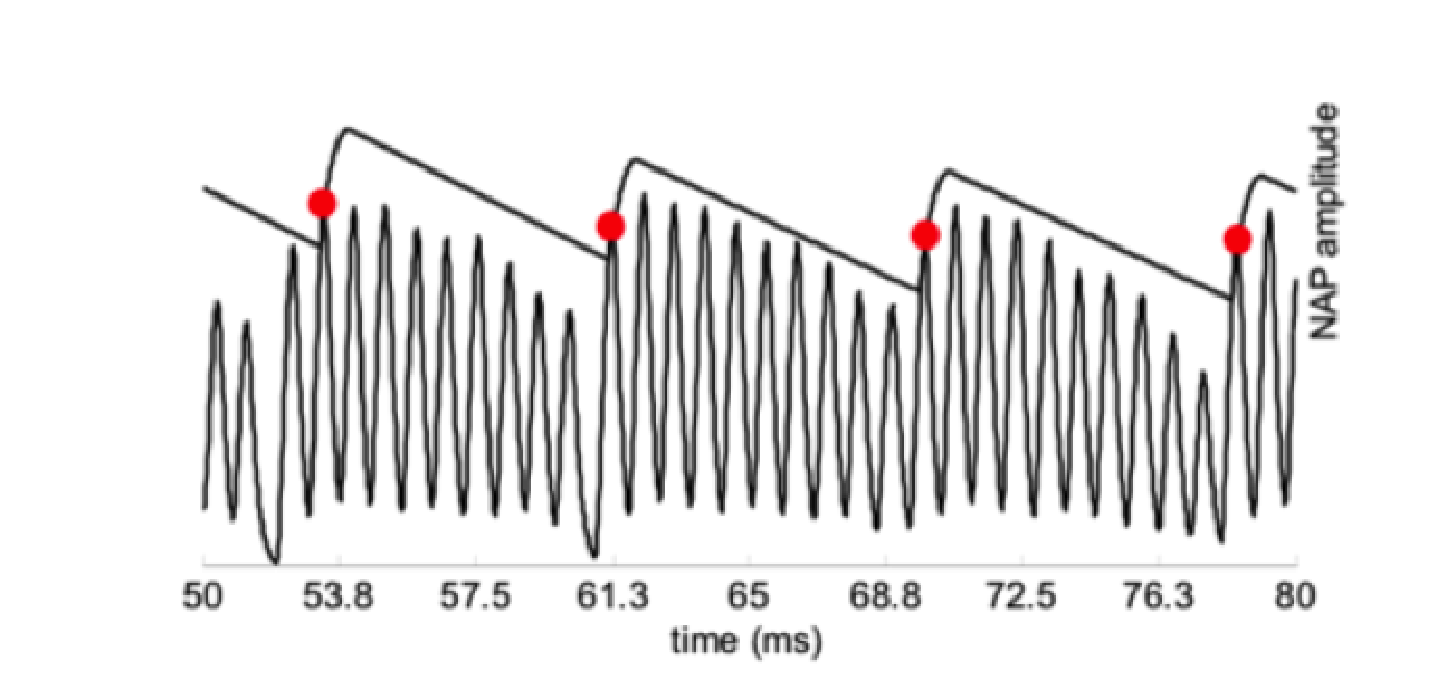
\includegraphics[width=100mm]{figures/triggerpoints}
\caption{ In this figure the solid black line in the center
  corresponds to the audio signal, and the red dots signify trigger
  points.  The solid black line at the top of the figure represents
  the current threshold value of the algorithm, and when this
  threshold crosses the line representing the audio, a new trigger
  point is generated.}
\label{fig:triggerpoints} 
\end{center} 
\end{figure} 

\begin{figure}[t]
\begin{center}
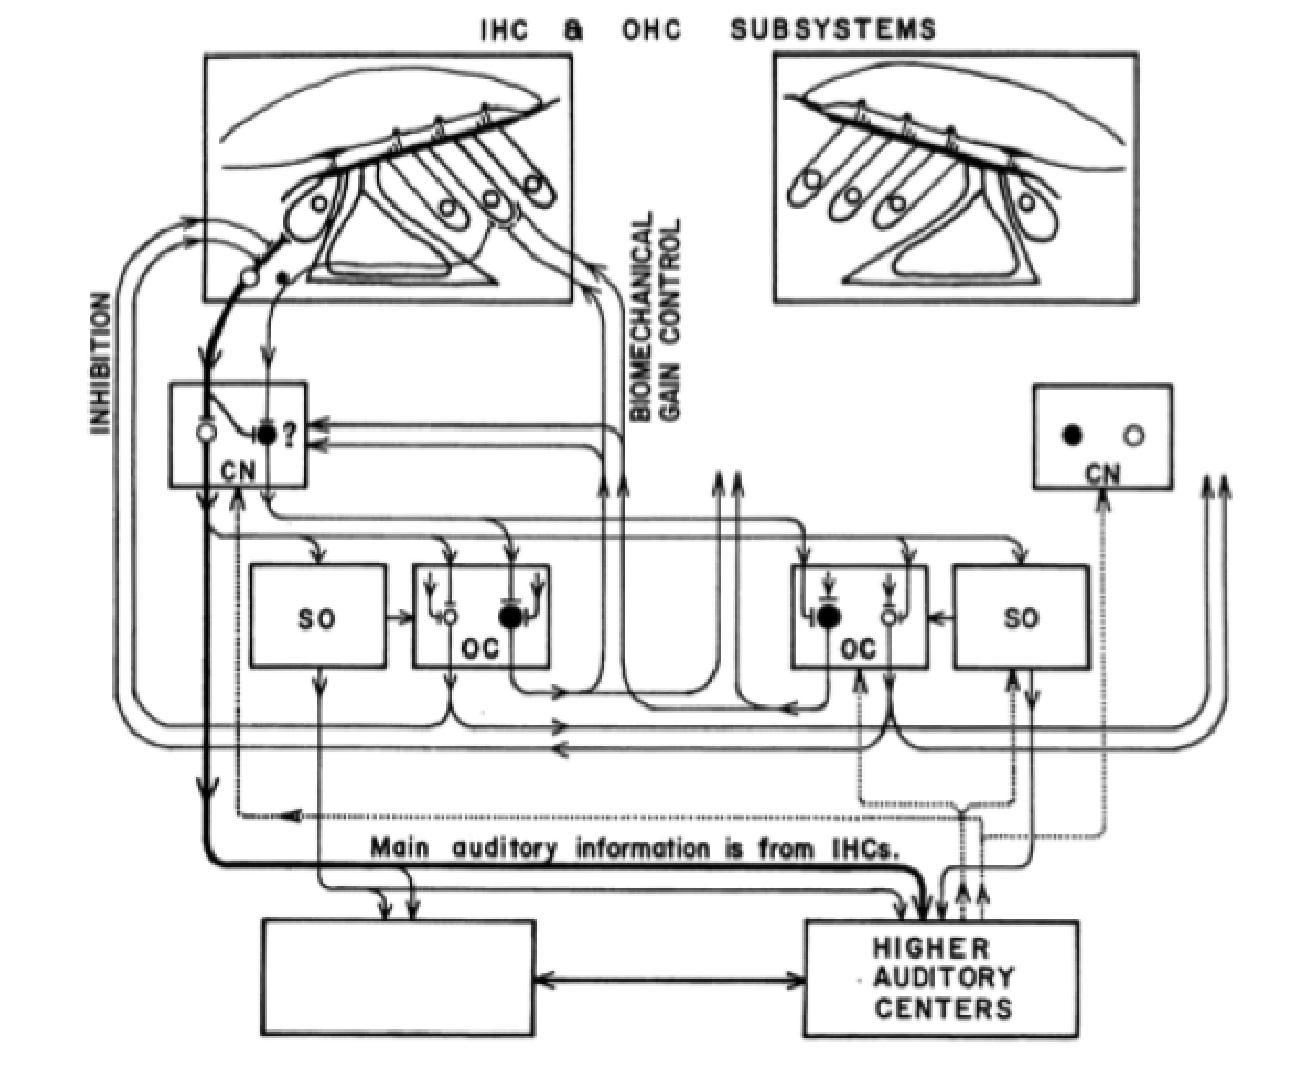
\includegraphics[width=100mm]{figures/ihcohc}
\caption{
A schematic view of the connections between the cochlea and the higher
levels of the auditory periphary, including connections between the
olivary complexes to each other and back to their respective cochleas.} 
\label{fig:ihcohc} 
\end{center} 
\end{figure} 


\section{Pitch Contour Extraction}  

The discrete calls of killer whales are pulsed signals in which a tone
(of a certain tonal frequency) is not emitted continuously but in
pulses given by the pulse-repetition rate. Unlike the tonal signals of
many birds and other delphinids, the highest energy is not always
contained in the first or second harmonic
\cite{deecke99_quantifying_orca}. The high levels of background noise
and variety of recording conditions compound the difficulty of
obtaining pulse rate contours. The pulse rate contour is used as the
primary representation for Orca calls because it is more robust as
compared to spectral features to levels of background noise typical in
field recordings.

We have compared three pitch extraction methods for obtaining the
pulse rate contour. The first method ({\bf PRAAT}) is based on
time-domain autocorrelation and is similar to the pitch extraction
algorithm implemented in Praat \cite{boersma93}. It is based on
calculating the time-domain autocorrelation of the signal:

\begin{equation} 
R(\tau) = \frac{1}{N} \sum_{n=0}^{N-1-m} x[n] x[n+m] \;\;\;\; 0 \leq m
< M 
\end{equation} 

The peaks of the autocorrelation function correspond to the lags 
in which the signal is self-similar. The signal is processed in
windows and the autocorrelation of the windowed signal $R_{xw}$ is divided 
by the autocorrelation of the window $R_{w}$ providing better robustness to 
noise and better accuracy. 

\begin{equation}
R_{x}(\tau) = R_{xw}(\tau) / R_{w}(\tau)
\end{equation} 

The second method is based on the {\bf YIN} pitch extraction method.
The YIN method is based on the difference function which is similar to
the autocorrelation:

\begin{equation}
d{t} = \sum_{n=0}^{N-1} (x[n] - x[n+\tau])^{2}
\end{equation} 

The dips in the difference function correspond to periodicities. 
In order to reduce the occurrence of subharmonic errors, YIN employs a
cumulative mean function which de-emphasizes higher period dips 
in the difference function. 

The third method ({\bf SACF}) is based on the multipitch detection
algorithm described by Tolonen and Karjalainen \cite{tolonen00}.  In
this algorithm, the signal is decomposed into two frequency bands
(below and above 1000 Hz) and amplitude envelopes are extracted for
each frequency band. The envelope extraction is performed by applying
half-wave rectification and low-pass filtering.  The envelopes are
summed and an enhanced autocorrelation function is computed so that
the effect of integer multiples of the peak frequencies to multiple
pitch detection is reduced.

We explore three retrieval strategies/representations. Statistical
features characterizing the entire pulse rate contour are computed and
each call is characterized by a single vector of features. The
features are normalized by max-min normalization so that they range
from 0 to 1 over the entire dataset. Similarities are then computed by
taking the Euclidean distance in the normalized space. This strategy
is used as reasonable baseline. The features used in this work are the
mean, median, standard deviation, min and max of the pulse rate
contour. The second strategy consists of resampling the pulse rate
contour using linear interpolation to a fixed number of points. This
strategy is similar to the one used in Deecke
\cite{deecke99_quantifying_orca}. Essentially it assumes that the
duration of the call does not play a major role in its
characterization and temporal scaling is applied uniformly across the
contour. The third strategy utilizes dynamic time warping to align the
pulse rate contours. The alignment cost is used to measure the
similarity between calls. The two sequences to be matched are arranged
on the sides of a grid. To find the best match between the sequences
we can find a path through the grid that minimizes the total distance
between them. More details can be found in \cite{sakoe78}.



\section{Machine Learning}
\label{section:softwareAndSystems:machineLearning}

In addition to the presentation and collaborative annotation that the
Orchive supports, we have also developed a set of Music Information
Retrieval and Machine Learning tools that are available for
researchers to run on the data in the Orchive. All of these tools are
part of the Marsyas \cite{marsyas} MIR framework

The first set of tools are audio feature extraction tools that have
been adapted from the field of Music Information Retrieval
(MIR) \cite{futrelledownie2002} to the study of orca vocalizations.
In particular we have added support for the generation of spectral
statistics including FFT spectrum, MFCC coefficients, Zero Crossing
Rate, Spectral Centroid, Flux and Rolloff.  In section 5.4 we detail
some results that were obtained using some of these features and show
that they perform well on this class of problems.

We also support classification of audio using Support Vector
Machines \cite{mandel-ismir2005}, an advanced type of Machine Learning
technique that finds optimal hyperplanes in high dimensional datasets,
which we then use to classify audio.  This classification can be as
simple as either ``orca'', ``voiceover'' or ``background'', or can be
as complex as classifying different call types or even different pods
through their call repertoires.  

One important design goal in this project is to make our system as
flexible and extensible as possible, to this end, we have come up with
a tag-based system that allows researchers to construct their own
ontologies.  Some of these ontologies would overlap, like ``orca'' or
``voiceover'', and some would be distinct to different areas of study.
By allowing a user defined structure to emerge, we empower individual
research communities to ask and answer the questions most pertinent to
them.  The obvious drawback to this is that within communities
researchers must agree on the same language and syntax to annotate
calls.  We hope to provide tools within and external to the site to
help encourage the collaboration necessary to converge on the same
vocabulary.

\subsection{Machine Learning}
\label{section:softwareAndSystems:machineLearning}

For this system, we used the support vector machine learning system
from libSVM which is included in the Marsyas\cite{marsyas} framework.
Standard Marsyas SVM parameters were used in order to classify the
sparse bag of auditory words representation of each song.  It should
be noted that SVM is not the ideal algorithm for doing classification
on such a sparse representation, and if time permitted, we would have
instead used the PAMIR machine learning algorithm as described in
\cite{lyon10}.  This algorithm has been shown to outperform SVM on
ranking tasks, both in terms of execution speed and quality of
results.

\section{Machine Learning}

\subsubsection{SVM}


\subsubsection{SOM}

For creating the visualization layout we utilized the self-organizing
map (SOM) which is a type of neural network used to map a high
dimensional feature space to a lower dimensional representation while
preserving the topology of the high dimensional space. This
facilitates both similarity quantization and visualization
simultaneously. The SOM was first documented in 1982 by T. Kohonen,
and since then, it has been applied to a wide variety of diverse
clustering tasks \cite{kohonen95a}. In our system the SOM is used to
map the audio features (64-dimensions) corresponding to each track to
two discrete coordinates on a grid.

The traditional SOM consists of a 2D grid of neural nodes each
containing a $n$-dimensional vector, $ {\bf x(t)} $ of data. The goal
of learning in the SOM is to cause different neighbouring parts of the
network to respond similarly to certain input patterns. The network
must be fed a large number of example vectors that represent, as
closely as possible, the kinds of vectors expected during mapping. The
data associated with each node is initialized to small random values
before training. During training, a series of $n$-dimensional vectors
of sample data are added to the map.  The ``winning'' node of the map
known as the {\it best matching unit} (BMU) is found by computing the
distance between the added training vector and each of the nodes in
the SOM. This distance is calculated according to some pre-defined
distance metric which in our case is the standard Euclidean distance
on the normalized feature vectors.

Once the winning node has been defined, it and its surrounding nodes
reorganize their vector data to more closely resemble the added
training sample.  The training utilizes competitive learning. The
weights of the BMU and neurons close to it in the SOM lattice are
adjusted towards the input vector. The magnitude of the change
decreases with time and with distance from the BMU. The time-varying
learning rate and neighborhood function allow the SOM to gradually
converge and form clusters


\section{Distributed Computing}


In order to analyze the audio in large online archives efficiently, a
scenario involving distributed computing must be used.  There are many
different types of systems that perform Machine Learning and many of
these can distribute their work to different machines.  Some of these
systems are better suited for this task than others, and in this paper
we investigate a few combinations of these tools.

One of the possible solutions to the problem of the segmentation of
audio into orca vocalizations and other sounds is to use a Machine
Learning supervised classifier system.  These systems require hand
labelled training data, in our particular case, audio would be
labelled as either orca or background.  This training data is then
used to train a classifier system that can classify future instances
based on features of the training data.  There are a wide variety of
classification algorithms that are commonly used, some of the most
popular are Support Vector Machines (SVMs), Neural Nets, Decision
Trees and Logistic Regression.  In our past work we have found good
success in using SVMs, and have shown that SVMs typically outperform
many other Machine Learning algorithms.  However, there is current
work in this area showing the benefits of many alternate algorithms
for different problem domains.

There are two steps to the problem of the classification of audio
signals.  The first is that of audio feature extraction, and the
second is that of classification with Machine Learning systems.  Sound
is a pressure wave in the air, and the variations in pressure over
time can be stored in a computer as real number values.  This raw
waveform data contains all the information of the signal, but because
of it's extremely high dimensionality, is difficult to analyze with
machine learning systems.  To take this raw data and to put it in a
form more conducive for analysis, we generate a large number of higher
level features, including spectral features \cite{marsyas}, pitch
information \cite{cheveigne02}, chromatic scale information
\cite{marsyas} and other features based on models of the auditory
cortex \cite{lyon82}.  One can also model the statistical behaviour of
these properties as they change over time, an avenue that has been
shown to be fruitful \cite{marsyas}.  In our system we investigated
the use of a number of audio features, the results of which are
discussed in the Evaluation section, but in summary we found that
using all the standard audio features was most useful, however using
pitch information degraded performance of the classifier.  This is a
surprising result and one that we are investigating further.

The second step is to take these audio features, train and test a
Machine Learning classifer on them, and then run this Machine Learning
classifier over all the data.  In many cases it is beneficial to
pre-calculate the audio features for the data, as once as good
parameters can be determined for the audio feature extraction engine,
such as the window size, hop size for the spectrum calculation and the
memory size for the windowed statistical calculations, these features
can be saved and reused in multiple Machine Learning experiments with
different parameters.  One example of this is the recent release of
the Echonest audio features for the Million Song Dataset
\cite{bertinmahieux11}.  This collection of audio features for one
million popular songs took a considerable amount of time to process,
and one approach is to save these audio features and running different
machine learning algorithms or different parameter sets of these
algorithms on them.  Another point that should be made here is that
the form of the features that are extracted in this step can have a
direct relation to the performance of the subsequent Machine Learning
step.  Different algorithms perform better with different forms of
data, and matching the right features to the right algorithm is both
an art and a science.

It should be noted that both of these steps, the audio feature
extraction and the Machine Learning could be carried out in the same
executable.  There are a number of advantages to this as well as some
disadvantages.  One major advantage is that the intermediate audio
feature data does not have to be saved on disk.  This intermediate
data can be very large in size, and can be many times larger in size
than the original audio data, depending on the type of compression
used for the original audio.  In many cases in the real world, it is
less expensive to just recalculate the audio features each time that a
new Machine Learning run is carried out rather than saving them on
disk.  This also can help to overcome any versioning problems, where
different versions of audio features are combined together in the
training, testing or predicting stages.  It will be a balance between
these two poles for production systems to manage.

For this work, Marsyas was used for doing Audio Feature Extraction.
There are other Music Information Retrieval toolkits for extracting
audio features, but the audio features output by Marsyas are typically
amongst the most robust and high performing in the literature
\cite{marsyas}.  We have implemented this feature extraction using
native filesystem operations loading data off of NFS or a local disk
depending on the cluster situation.

For the Machine Learning half of the project, a variety of Machine
Learning systems and algorithms were used and comparison of them in is
provided in the evaluation section.  Results have been produced for a
Logistic Regression system using a Stochastic Gradient Descent
algorithm on Mahout, a distributed Machine Learning system implemented
as a Java library on top of Hadoop, an open source clone of the Google
File System (GFS) and Google MapReduce system.  These results are
compared to a Logistic Regression system using a quasi Newton solver
as implemented in Weka, a popular system for Machine Learning and show
timing and classification results of this system run as a grid style
parallel job on Westgrid.  These results for Logistic Regression are
then compared to three different implementations of a Support Vector
Machine (SVM) classifier.  The first of these is simply the SVM mode
in Weka but run in a grid-style distributed manner.  The second of
these is a parallel version of the SVM algorithm, PSVM
\cite{chang07psvm}.  The third of these is a hybrid audio feature
extraction and SVM developed in the Marsyas framework.  These three
different systems will be compared and contrasted in the Evaluation
section.

I propose to use the Westgrid system for running the huge audio
feature extraction task. This uses a very simple queuing system known
as Torque, which is the latest evolution of the ancient PBS (Parallel
Batch System) parallel job distribution system. PBS allows scientific
users to schedule large jobs to run on computers, and performs well
for certain scientific tasks where a single, usually large, program is
run on a variety of different datasets, and the results are then saved
to disk and later analyzed by a scientist. This type of computing was
traditionally known as Grid Computing.  While this system has certain
benefits for running specific scientific tasks, for other tasks, the
methodology of having separate computers running mostly independently,
and all coordination of tasks being the responsibility of the
programmer with an tool such as MPI quickly becomes difficult. The
MapReduce paradigm helps in the coordination of large parallel tasks,
and the Hadoop system allows programmers to efficiently write
distributed programs that run on huge numbers of computers and allows
for failures of individual computers. In this project we will use the
Mahout Machine Learning framework on top of a Hadoop installation to
process the audio feature vectors output by Marsyas and to gain
insights into the vocalization data in the Orchive. The primary task I
will investigate in this project will be identifying regions of the
Orchive with distinct orca vocalizations that are nearby to
hydrophones and isolated from other orca vocalizations.

Mahout is a Machine Learning framework that interacts closely with
Hadoop to both store the data and also run the Machine Learning
algorithms.  Hadoop is an open source port of the GFS
\cite{ghemawat03} and MapReduce \cite{dean08} infrastructure and
allows users to run large jobs that follow the map reduce paradigm.
In this scheme, a parallel job is split into two phases, a map phase
and a reduce phase.  In the map phase, key value pairs are generated
by some given algorithm from an input file, this same process occurs
in parallel on many other nodes, and the data that is used by a given
map is determined by the locality of data on that node.  These key
value pairs are then sorted and shuffled to a set of reduce nodes,
which take the collections of key value pairs and do an operation on
them that in some way combines, or reduces, the data.  These map and
reduce functions can be thought of as similar to the map and reduce
functions in functional programming, however, it should be noted that
this is a loose similarity due to the lack of higher order functions
in the current MapReduce implementation.  Many algorithms have been
ported to use this MapReduce type system, some of the most natural are
those that process large collections of text for building inverted
indexes or other tasks for searches, which is not surprising noting
the provenance of the MapReduce algorithm.  For other tasks, such as
those common in audio feature extraction, the reduce phase is simply
an identity reduce, where the map outputs are copied verbatim to the
reduce outputs.  It is easier and more natural to make some algorithms
more efficient in a MapReduce context than others.

The Mahout Machine Learning framework has implemented many different
Machine Learning algorithms in it's framework, including clustering,
recommendation and classification algorithms.  In our current work we
are more interested in classification than either recommendation or
clustering, and Mahout boasts support for the following classification
algorithms: Logistic Regression (SGD), Bayesian, Support Vector
Machines (SVM), Perceptron and Winnow, Neural Network, Random Forests,
Restricted Boltzmann Machines, Online Passive Aggressive, Boosting and
Hidden Markov Models.  However, after investigation, it appears most
of these algorithms are in a definite alpha state, and require
patching of the main source tree with external files.  The two most
well supported classification algorithms in Mahout are the Logistic
Regression classifier, using a Stochastic Gradient Descent (SGD)
engine, and a Naive Bayesian classifier.  Upon extensive
investigation, the Bayesian classifier makes many internal assumptions
of the input being of large bodies of written text and was not
suitable for our use case.  However, the Logistic Regression
classifier was well suited to our data and performed well in our
tests.

One advantage of using the Mahout Machine Learning framework was that
it stored its input and output data on HDFS, the Hadoop Distributed
Filesystem.  When working with the huge amounts of data that are
generated by audio feature extraction and Machine Learning
experiments, managing and transferring experimental results from the
grid servers to the production web servers is often a time consuming
and error prone procedure.  After our experience with Hadoop, we have
integrated it into web application and use the WebHDFS system to serve
all experimental results to users.  These users interact with a web
application that displays some data obtained from the production web
server but also displays the results of experiments as data served
live from a WebHDFS system that is being populated by the experimental
results from live requests from scientists.


%%%%%%%%%%%%%%%%%%%%%%%%%%%%%%%%%%%%%%%%%%%%%%%%%%%%%%%%%%%%%%%%%%%%%%%%%%%%%%%%
%%%%%%%%%%%%%%%%%%%%%%%%%%%%%%%%%%%%%%%%%%%%%%%%%%%%%%%%%%%%%%%%%%%%%%%%%%%%%%%%
%% Chapter - Case Studies
%%%%%%%%%%%%%%%%%%%%%%%%%%%%%%%%%%%%%%%%%%%%%%%%%%%%%%%%%%%%%%%%%%%%%%%%%%%%%%%%
%%%%%%%%%%%%%%%%%%%%%%%%%%%%%%%%%%%%%%%%%%%%%%%%%%%%%%%%%%%%%%%%%%%%%%%%%%%%%%%%


\startchapter{Case Studies}
\label{chapter:caseStudies}


\section{Introduction}\label{sec:introduction}

There are a number of large bioacoustic archives that have been
described in the literature, and as computer storage grows ever
larger, more of these archives are being created.  In this work, we
will focus on two such large bioacoustic datasets, The Orchive, and
the recordings made by the Alberta Biodiversity Monitoring Institute
(ABMI).  The Orchive is an archive of sounds collected by a network of
stationary, permanently mounted hydrophones, and the primary sound
that was of interest to the researchers was that of Orcas.  The ABMI
dataset is collected at a series of 1700 sites in Alberta using
a specialized stereo microphone device.

While these two datasets on the surface would appear to be very
different, the underlying data collected by both is audio, and the
tools to study both these sources of data are in large part very
similar.  These tools include a web-based interface to allow
researchers to listen to, view and annotate this audio, tools to
extract and view audio features from this data, and tools to run
machine learning software and view the results of this analysis.


\section{The Orchive}\label{sec:the_orchive}

The whale species \emph{Orcinus orca}, commonly known as Killer Whales
\cite{ford00_book_killer_whales}, are large toothed whales found
around the world, in places as far afield as Antarctica and
Alaska\cite{estes09_orca_alaska_decline}.  The vocalizations of orcas
are complex and diverse, and consist of a wide variety of
vocalizations, which include echolocation clicks, tonal whistles and
pulsed calls \cite{deecke00}. There are stable resident populations of
Orcinus Orca in the northwest Pacific Ocean, some of these populations
are found near Hanson Island, off the north tip of Vancouver Island in
Canada.  There are three distinct types of Orcas, Transients,
Residents and Offshores, each of which have different feeding
behaviours and different styles of communication.

Orcalab is a research station that has been recording audio of these
Orca populations since 1972 \cite{weiss06}.  
 It was designed as a land based
research station in order to reduce the impact of the researchers on
the orcas under study, as the noise and disturbance from boats impacts
the orcas in observable but currently unquantified ways.

They have amassed a huge
archive of more than 20,000 hours of audio recordings collected via a
permanent installation of underwater hydrophones.  It contains a
continuous archive of orca vocalizations from the 1980 to the present
time.  This archive of data is very large, and the sound files that it
contains occupy approximately 15TB of disk space.  The archive was
recorded onto cassette and DAT tapes.  

The vocalizations of orcas are recorded through a series of
hydrophones, microphones that are designed specifically to work under
the water.  A few of the hydrophones are hardwired, but in order to
have greater geographical reach, most of the hydrophones operate
remotely, transmitting their recordings via VHF radio to the main lab.
These signals are then fed into a 6-channel mixing console.  The
researchers continuously adjust the levels of the recordings both to
increase the volume of the hydrophone located closest to the orcas,
and also to decrease the volume of any hydrophones that are close to
sources of boat noise.

Our lab here at the University of Victoria has been collaborating with
OrcaLab for approximately 6 years, and in this collaboration we have
just recently completed the process of digitizing the collection of
analog and DAT tapes.

Although these recordings contain large amounts of Orca vocalizations,
the recordings also other sources of audio, including voice-overs
describing the current observing conditions, boat and cruise-ship
noise, and large sections of silence.  Finding the Orca vocalizations
on these tapes is a labor-intensive and time-consuming task.

Many parts of the recordings contain boat noise which makes
identifying orca calls both difficult and tiring. In addition, the
size of the Orchive makes full human annotation practically
impossible. Therefore we have explored machine learning approaches to
the task. One data mining task is to segment and label the recordings
with the labels background, orca, voice. Another is to subsequently
classify the orca calls into the classes specified in the call
catalog.

The goal of the Orchive project is to digitize acoustic data that have
been collected over a period of 36 years using a variety of analog
media at the research station OrcaLab (\url{http://www.orcalab.org})
on Hanson Island on the west coast of Vancouver Island in
Canada. Currently we have approximately 20000 hours of analog
recordings, mostly in high quality audio cassettes. In addition to the
digitization effort which is underway, we are developing algorithms
and software tools to facilitate access and retrieval for this large
audio collection.  The size of this collection makes access and
retrieval especially challenging (for example it would take
approximately 2.2 years of continuous listening to cover the entire
archive).  Therefore the developed algorithms and tools are essential
for effective long term studies employing acoustic
techniques. Currently such studies require enormous effort as the
relevant acoustic tapes need to be recovered and the relevant segments
need to be tediously digitized for analysis.

The majority of the audio recordings consist of three broad classes of
audio signals: background noise caused mainly by the hydrophones,
boats, background noise containing orca vocalizations and voice over
sections where the observer that started the recording is talking
about the details of the particular recording. In some cases there is
also significant overlap between multiple orca vocalizations. The orca
vocalizations frequently can be categorized into discrete calls
\cite{ford89} \cite{ford91} that allow expert researchers to identify
their social group (matriline and pod) and in some cases even allow
identification of individuals.

Even when the data is digitized, locating a particular segment of
interest in a long monolithic audio recording can be very tedious as
users have to listen to many irrelevant sections until they can locate
what they are looking for. Even though visualizations such as
spectrograms can provide some assistance this is still a task that
requires much manual effort. In this paper we describe experiments for
the automatic classification and segmentation of the orca recordings
for the purposes of locating segments of interest and facilitating
interaction with this large audio archive.

An important aspect in the design of a tool to support collaborative
work is to consider what user communities will use the tool.  In the
case of the Orchive, there are a number of different scientific
communities that will be using this tool and the data this tool
provides access to.  The primary scientific community that will
benefit from this work will be cetacean biologists.  In order to study
the rich archive orca vocalizations that have been recorded by
Orcalab, researchers must currently travel to Hanson Island, search
through the lab books and incidence reports to find which recordings
contain the data they are interested in, locate the physical cassette
tape corresponding to this recording, and then either manually listen
to the tape, or perhaps digitize the tape and analyze it in the
computer.  Each researcher typically then keeps the annotations and
data generated from this procedure themselves, if future researchers
want to obtain this data for further analysis, they must first be
aware of the fact that this researcher has the data, and then request
it from them.  With the distributed collaborative system we have
designed, not only can these biologists easily listen to any recording
in the entire archive from any internet connected computer in the
world, and compare different recordings, they can also add their
annotations to the system.  These annotations can be either private or
public, if they are for use in a publication, after the article has
been accepted for publication, the researcher can make their private
annotations public.  These researchers are less interested in the
details of audio feature extraction and machine learning algorithms,
and are instead more focused on asking biologically informed
questions, like dialect change in cetacean call repertoire
\cite{deecke00}.

Another scientific community that will receive benefits from this
archive are the developers of bioacoustic algorithms.  These
scientists are typically computer scientists with interests in Music
Information Retrieval and bioacoustics.  This archive represents a
site where researchers can get large amounts of high quality and
uniformly collected data.  Researchers interested in bioacoustic
algorithms have different goals and skill sets from cetacean
biologists, for example, many have extensive knowledge of Digital
Signal Processing and audio feature extraction algorithms.  This
system should be flexible and powerful enough to allow these
researchers to ask questions that are relevant to them.  The required
features for this group of users include allowing them to choose
different audio feature extraction algorithms, and to then take the
resulting data and run it against a variety of machine learning
algorithms in as flexible a manner as possible.

Another group of scientists that have expressed interest in the
Orchive are Environmental and Conservation scientists. A research
question particular interest is the effect of boat noise
\cite{foote04} on cetaceans and on the marine
environment in general.  For these researchers, the data they will be
most interested in is the frequency and nature of orca vocalizations,
and the intensity and spectral characteristics of boat noise
\cite{holt09}.  There are large differences in the
intensity and frequency content of boat noise depending on the type of
boat that creates it, speed pleasure craft often create a high pitched
noise that quickly moves away, tug boats have a lower pitched sound
and take a long time to move through an area, and cruise ships make a
loud and distinctively high pitched sound.  Analyzing the effects of
these various types of boat noise will help researchers to establish
guidelines for boat noise as it affects this sensitive population of
marine mammals \cite{doksaeter09}.

Another group of scientists that this work will benefit are those
studying the social organization of whale communities
\cite{bigg90_orca_genealogy}.  There have been studies that
investigate the transmission of culture in orca societies
\cite{deecke00} and have found evidence of this through the
examination of dialect change.  In a similar vein, other studies have
investigated social learning \cite{janik00_orca_social_communication}
in communities of orcas.  With a large database such as this, more of
these type of studies will be made possible in the future.

In this work we design a series of Machine Learning systems to examine
and classify various aspects of this archive.  We first look at
classifying different recordings based on how much noise is present in
each recording.  There is often considerable boat noise in the
recordings, and in many cases this makes analysis difficult or
unfeasible.  By identifying recordings with less boat noise, we can
narrow the amount of data that is required to be analyzed by humans
and machine learning systems.

The second task in this work is to develop machine learning systems to
pull out individual orca calls from recordings.  These systems should
discriminate between background noise, orca calls and the voice notes
that are present in most of the tapes in the orchive.  Once we have
identified clips containing orca vocalizations, the third task in this
work is to classify these calls based on a previously existing call
catalog, first developed by John Ford.


Most of existing work in the automatic analysis of Orca calls has
focused on detection and classification rather than retrieval. A
real-time system with low computational requirements for the detection
of Orca vocalizations is described in \cite{Luke2010771}. Annotation
bootstrapping is a technique used to classify/segment hydrophone
recordings into three broad categories: voiceover, background, and
vocalizations \cite{ness08}. 

Over the past 5 years, a number of orca researchers using our website
have added over 18,000 clip annotations to our database.  A small
section of annotated audio from the Orchive is shown in Figure
\ref{fig:dm_orchive}.  These clip annotation are of two main types:
The first is clips that differentiate background noise from orca calls
and from the voice notes of the researchers that collected the data.
The second type of clip annotations classify orca vocalizations into
different calls.  Orcas make three types of vocalizations,
echolocation clicks, whistles and pulsed calls.  The pulsed calls are
highly conserved stereotyped vocalizations which have been classified
into a catalog of over 52 different calls by John Ford \cite{ford87}.
Of the 18,000 annotations currently in the Orchive, 3000 are of these
individually classified calls.  In addition, we have a curated call
catalog containing 384 different recordings of different calls
vocalized by a variety of different pods and matrilines. This catalog
is used for training the annotators.


The goal of the Orchive project is to digitize acoustic data that have
been collected over a period of 36 years using a variety of analog
media at the research station OrcaLab (\url{http://www.orcalab.org}) on
Hanson Island on the west coast of Vancouver Island in
Canada. Currently we have approximately 20000 hours of analog
recordings, mostly in high quality audio cassettes. In addition to the
digitization effort which is underway, we are developing algorithms and
software tools to facilitate access and retrieval for this large audio
collection.  The size of this collection makes access and retrieval
especially challenging (for example it would take approximately 2.2
years of continuous listening to cover the entire archive).  Therefore
the developed algorithms and tools are essential for effective long
term studies employing acoustic techniques. Currently such studies
require enormous effort as the relevant acoustic tapes need to be
recovered and the relevant segments need to be tediously digitized
for analysis.

The majority of the audio recordings consist of three broad classes of
audio signals: background noise caused mainly by the hydrophones,
boats, background noise containing orca vocalizations and voice
over sections where the observer that started the recording is talking
about the details of the particular recording. In some cases there is
also significant overlap between multiple orca vocalizations. The orca
vocalizations frequently can be categorized into discrete calls that
allow expert researchers to identify their social group (matriline and
pod) and in some cases even allow identification of individuals.

Even when the data is digitized, locating a particular segment of
interest in a long monolithic audio recording can be very tedious as
users have to listen to many irrelevant sections until they can
locate what they are looking for. Even though visualizations such as
spectrograms can provide some assistance this is still a task that requires much
manual effort. In this paper we describe experiments for the automatic
classification and segmentation of the orca recordings for the
purposes of locating segments of interest and facilitating interaction
with this large audio archive.

Because the researchers from Orcalab have devoted so much time and
care to the recording and documenting the audio in the Orchive, an
important design criteria is to ensure that data entered from
non-specialist users will not interfere with the data from expert
users and scientists.  To this end, we have implemented a reputation
management and filtering system, along with roles for various users.

In the current implementation of the Orchive, only expert scientists
are allowed to make annotations, and only members of Orcalab and their
collaborators are allowed to edit the start date of each recording.
As well, users can choose exactly which user's annotations they want
to view.  In light of the fact that everyone in the current user
community knows each other personally, reputation management is
handled by offline personal interactions.  When the general public is
allowed to contribute using a crowdsourcing model, this system will be
expanded and enhanced.


\section{ABMI}\label{sec:abmi}

Another rich source of bioacoustic data comes from the Alberta
Biodiversity Monitoring Institute (ABMI).  The ABMI is a non-profit
organization that collects, analyzes and reports on the status of
biodiversity in the province of Alberta.  It is one of the largest and
most systematic such biodiversity projects in the world, and is widely
regarded as a leader in biodiversity monitoring.  It has the goal of
refining, analyzing, and synthesizing raw data make it more meaningful
for politicians, policy makers and managers to use.

The ABMI surveys 1656 evenly spaced monitoring sites across Alberta,
and visits 330 sites each year, and surveys the entire province every
5 years.  There are 80,000 species of wildlife in Alberta. About 2000
(< 2\%) of these species are vertebrates, and vascular and
non-vascular plants, and it is these 2000 species that are monitored
by the ABMI.  During these surveys, a team of two researchers make
detailed observations of the site, collect samples for later
identification, and of most relevance to this project, make high
quality audio recordings of the site, which are later analyzed by
highly trained researchers in bird identification.

It is important to measure biodiversity because in order for policy
makers to make informed decisions when it comes to areas of
sustainable resource management, it is necessary to first measure and
quantify the current state of biodiversity, and to measure the changes
in biodiversity that happen during projects.  In order to do this,
there is a need for a solid evaluation method for biodiversity that is
objective and rigorous to evaluate changes in biodiversity. The ABMI
monitors changes in highly relevant species and uses a pyramid
framework for aggregating data \ref{fig:abmiInfoPyramid}.  This
pyramid has at its base the primary data, this is synthesized in
progressively higher levels of abstration to the state of individual
species, specific guild-level indices, general guild-level indices, to
taxonomic indices and finally to a single index.  Every year, this
single index is further summarized into an annual report that
describes broad changes in biodiversity in the province of Alberta.
The communication of results is of primary importance in this project,
and all results are freely available to all interested parties.

The ABMI was designed to increase efficiency by using a cost-shared
operational model which reduces duplication of effort and it benefits
many sectors of the economy including forest sector, energy sector,
agricultural sector, the public, the government and the scientific
community

Biological diversity (biodiversity) can be defined as the variability
among living organisms from all sources including terrestrial and
aquatic ecosystems.  At a broader level, this includes the the
ecological complexes of which they are part, and the diversity within
species, between species, and of entire ecosystems.  Biodiversity is a
shared responsibility of at least 17 different agencies in Alberta,
and the ABMI functions as a central repository of data on biodiversity

Cumulative-effects monitoring approach that is targeted at detecting
the ecological effects of a diverse set of environmental stresses on
broad suites of indicators \cite{manley04}. Cumulative-effects
monitoring exposes correlative relationships between stressors in a
system and the many indicators that are monitored \cite{thornton94}

ABMI assesses the performance toward management objectives such as
``regional sustainability'' or ``ecological integrity''
\cite{mulder99}. This monitoring approach remains relevant over long
timeframes as new human activities and environmental stresses are
introduced to landscapes \cite{watson04}.

The province of Alberta is 661,000 km2 and makes up 6.6\% of
Canada. Alberta has 6 major Natural Regions (Natural Regions Committee
2006). The Rocky Mountain Natural Region makes up 7\% of Alberta and
is dominated by rock, icefields, and coniferous forest. The Foothills
Natural Region makes up 10\% of Alberta and is dominated by rolling
topography with deciduous, mixedwood, and coniferous forests. The
Grassland Natural Region makes up 15\% of Alberta and is dominated by
grasses and shrublands. The Parkland Natural Region makes up 9\% of
Alberta and is dominated by deciduous forests and willow
shrublands. The Boreal Forest Natural Region makes up 58\% of Alberta
and is dominated by deciduous, mixedwood, and coniferous
forests. Finally, the Canadian Shield Natural Region makes up 1\% of
Alberta and is dominated by exposed bedrock, and open deciduous and
coniferous forests.

The ABMI does a systematic and unbiased sampling scheme to survey
biota and habitats.  In addition, for a given sampling effort,
creating a series of panels and surveying one panel each year,
achieves higher statistical power than having fewer locations and
surveying all locations each year \cite{urquhart98} \cite{urquhart99}.

The ABMI uses many raw data sources for it's reports, including field
notes of physical site characteristics, tree cores, plant samples and
photographs, but the data source of interest in this thesis are the
audio recordings of birds at each site.

These bird recordings follow a detailed protocol which each team is
trained to follow.  For each site, there are 9 different recordings
that are taken.  These recordings are done in a grid pattern, starting
at the site location, with each subsequent recording done 300 meters
from the last, in a proscribed fashion as shown in Figure \ref{}.  The
bird recordings are begun approximately 30 minutes before sunrise, and
during the recording, the person doing the recording is instructed to
listen on headphones during the entire recording to ensure it is
recorded.  The second member of the team is instructed to remain
silent during the recording to not disturb the birds and to avoid
noise that could be heard on the recording.  The recordings are done
with an advanced omnidirectional microphone well suited to recording
birds, and will be described in detail below.  The recording levels
are standardized so recordings are comparable and to avoid potential
for poor recordings, the recording level is set based on the value for
the particular model of microphone being used, this setting is used
consistently among sites regardless of wind or environmental
conditions.

All recordings are made at 320 kbps or greater sampling rate, which
means that the maximum frequency that can be recorded is 160kHz, which
captures most of the main frequencies and harmonics of birds.

At the beginning of each recording the person doing the recording is
asked to state their name, crew number, date, site number, point count
station number and the start time, this is followed by a standard tone
that is at least 5 seconds in duration, which is used to standardize
recording intensity.  During the 10 minutes in which the recording is
being made, the recordist scans the surrounding area using binoculars,
and for all birds observed they state the species identity, number of
individuals, and distance they are from the microphone so that this
information is also recorded.

To ensure data is not lost, the 9 bird recording files are digitally
copied to a laptop computer or portable hard drive at the end of each
day, and all recordings are saved on the recorder as well as on the
laptop for backup in the field.  At the end of each field shift, bird
recordings are transferred to the lab.  To maximize detections of
birds surveyed are conducted between May 25 and June 22.  

The omnidirectional microphone that is used in these recordings is an
advanced CZM microphone, which can be seen in Figure \ref{fig:czm1}.
This microphone has a 360 degree radial pattern and provides a forward
sound pressure gain comparable to a 24-inch parabolic microphone.  The
CZM microphone is a radially directional acoustical microphone which
is designed to simultaneously receive both direct and reflected sound
waves at its boundary.  These sound waves are then compressed as they
move through the flat plane of the microphone enclosure toward the
microphone diaphragm.  It increases the signal-to-noise ratio by 14
db, by using a wave guide design.  This wave guide design is shown in
Figures \ref{fig:czm2} \ref{fig:czm3}.

These recordings are then analyzed by a highly trained team of experts
in bioacoustics and bird identification.  The tools that are used by
these experts are standard programs which include Audacity
\cite{audacity} for listening to and viewing the sound, Microsoft
Excel for entering data, and a variety of web browser windows that
have example clips of bird vocalizations, common birds in the study
area, and other types of information about these birds.  The process
for listening to and identifying bird vocalizations using these tools
is cumbersome, and recently we were contacted by the head of this team
to help design custom software to help with this process.  We
subsequently obtained funding from the ABMI to develop a tool to help
with this process.

In this thesis, we describe a software system that we designed in
collaboration with this expert to help him and his team perform the
task of identifying bird species in these recordings.  This tool
incorporates a considerable amount of the code and tools designed for
the Orchive interface, and the additions made this tool in the course
of the ABMI project has made it more flexible and capable of dealing
with different forms of audio data.  We present results from a
iterative development process in which we co-created a tool with the
experts from the ABMI that allowed them to listen to, view and
annotate this large bioacoustic archive in a collaborative manner.  In
addition, preliminary results of automated identification of birds
from these recordings is presented.

This development process highlights the importance of developing
highly interactive tools that empower experts using technology
designed with their workflow and needs in mind.  While it is possible
to use standard tools to do this, the use of customized tools can
greatly speed up the process of species identification. 


\begin{figure}[h]
\centering
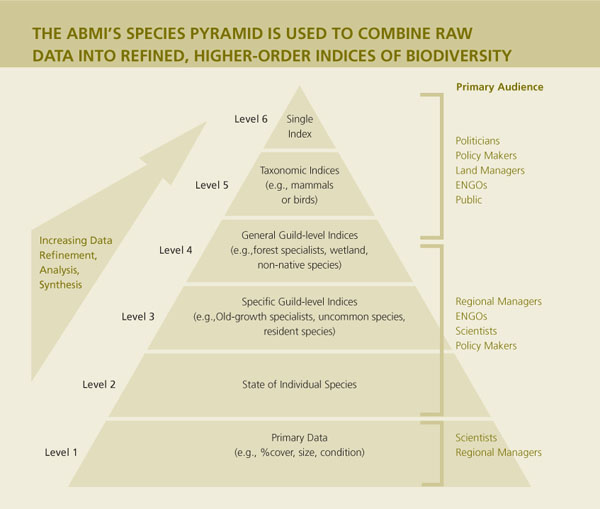
\includegraphics[width=90mm]{figures/abmiInfoPyramid.jpg}
\caption{abmiInfoPyramid}
\label{fig:abmiInfoPyramid}
\end{figure}

\begin{figure}[h]
\centering
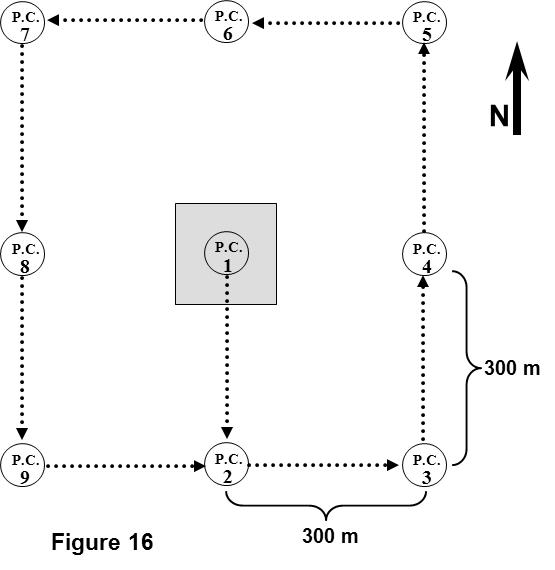
\includegraphics[width=90mm]{figures/abmiGrid.jpg}
\caption{abmiGrid}
\label{fig:abmiGrid}
\end{figure}

\begin{figure}[h]
\centering
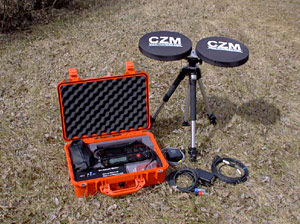
\includegraphics[width=90mm]{figures/czm1.jpg}
\caption{czm1}
\label{fig:czm1}
\end{figure}

\begin{figure}[h]
\centering
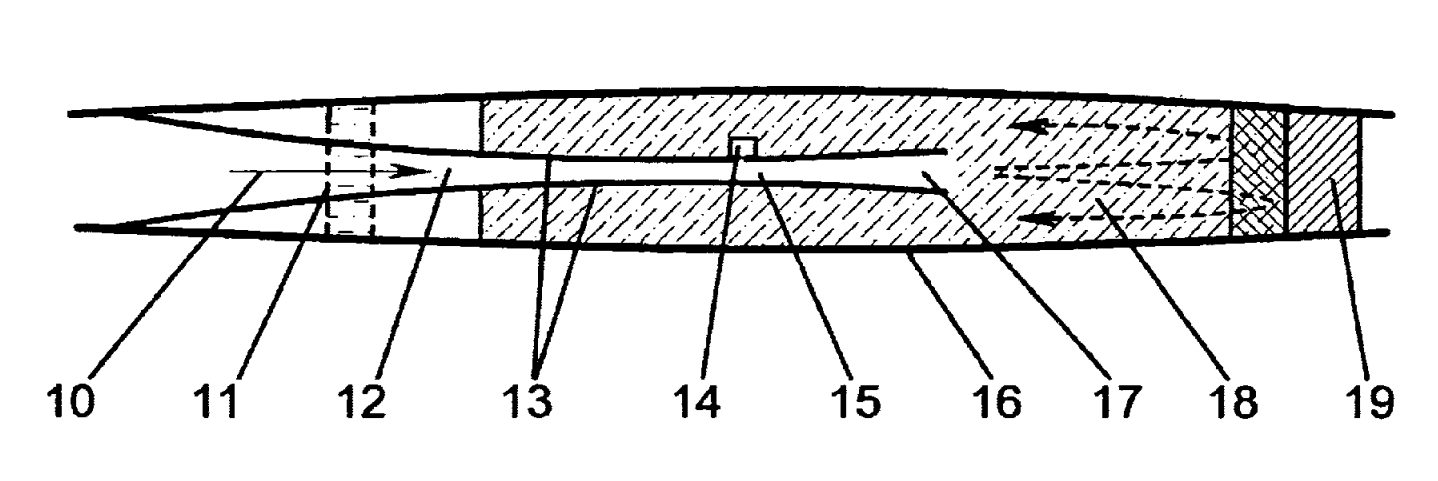
\includegraphics[width=90mm]{figures/czm2.png}
\caption{czm2}
\label{fig:czm2}
\end{figure}

\begin{figure}[h]
\centering
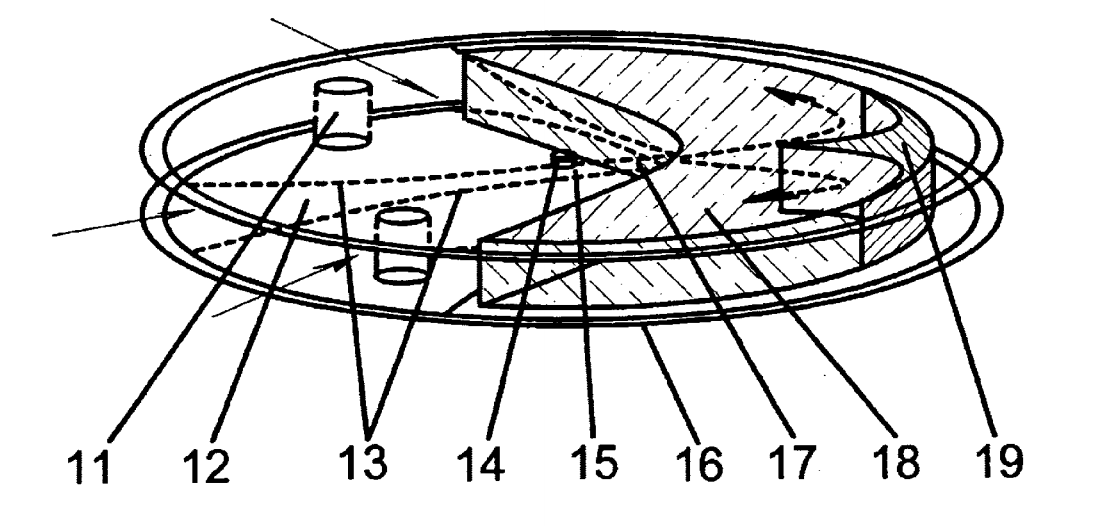
\includegraphics[width=90mm]{figures/czm3.png}
\caption{czm3}
\label{fig:czm3}
\end{figure}




%%%%%%%%%%%%%%%%%%%%%%%%%%%%%%%%%%%%%%%%%%%%%%%%%%%%%%%%%%%%%%%%%%%%%%%%%%%%%%%%
%%%%%%%%%%%%%%%%%%%%%%%%%%%%%%%%%%%%%%%%%%%%%%%%%%%%%%%%%%%%%%%%%%%%%%%%%%%%%%%%
%% Chapter - Evaluation
%%%%%%%%%%%%%%%%%%%%%%%%%%%%%%%%%%%%%%%%%%%%%%%%%%%%%%%%%%%%%%%%%%%%%%%%%%%%%%%%
%%%%%%%%%%%%%%%%%%%%%%%%%%%%%%%%%%%%%%%%%%%%%%%%%%%%%%%%%%%%%%%%%%%%%%%%%%%%%%%%

\startchapter{Evaluation}
\label{chapter:evaluation}

The final goal of the work in this thesis is to take the raw audio
obtained from large scale recording projects and to find and label the
audio events made by the organisms that are being studied.  In the
case of the Orchive, these are in general the various vocalizations of
orcas, and more specifically are the stereotyped pulsed calls.  For
this project, the final goal would be to assign call types to each
vocalization from the call catalog of Ford \cite{ford87}, and to label
the clan, pod, subpod, matrilinial association of the orca making
these calls.  The difficulty of assigning each call to a group of
whales becomes more difficult as more specific groups of whales are
considered, and varies considerably for each call type.  For example
the N47 call is made exclusively by the A1 pod of whales, so if this
call is detected, the identity of the pod making this vocalization can
be assigned at the same time.  In addition, there is considerable
variation in the prouction of the N47 by different matrilines (A12,
A30, A34, A36), so the assignment of matrilinial identity to this call
could also be possible.  Other calls, like the N03 call, are made by
all the pods in the A clan (A1, A4, A5, B, C, D, H, I1) and has little
variation between the different pods, so assigning this call to a
specific pod or matriline is difficults

In the case of the ABMI, these are the calls and songs of the birds
that could be extant in Alberta in the period of the study session.
For the calls of different species, the short time of each call, and
the similarity between calls of different species makes this a
challenging classification task.  The songs of birds have more
variation and are of longer duration, and are easier to classify.
Birds that are taxonimally related to each other make similar sounds,
for example the Swainsons thrush and the Hermit thrush have very
similar songs, but differ in the raspiness of the first note of their
song, which could be an identifying feature for machine learning
systems to identify.  

The process of classification of audio involves three major steps, the
first being the labelling of audio with ground truth by experts, audio
feature extraction of audio, and the use of machine learning to
classify the audio features with the ground truth labels from
experts.  

For the labelling of audio, a web based system was developed for this
thesis that allowed experts to listen to, view and label audio data.
This system allowed for the use of very large corpora of audio, with
long audio files of 45 minutes in length and greater.


For audio feature extraction, the primary toolkit that was used was
the Marsyas \cite{marsyas} framework, an extensible system based on a
data flow metaphor containing subsystems that allowed for the
computation of many different audio features.  It also contained low
level subsystems that allowed for new audio features to be quickly
implemented.

In the course of work done for this thesis, this author added new
audio feature extraction subsystems to Marsyas, including the porting
of the Yin pitch detector from Aubio to Marsyas, the porting from
MATLAB of the various subsystems required for the calculation of
Stable Auditory Images (including the Pole Zero Filter Cascade,
Gammatone filterbank, CARFAC, Halfwave Rectification, Stable Auditory
Image, Scale Stabilized Auditory Image, Box cutting, and Vector
Quantization), and the development and implementation of a Sideband
Interval detector.

For machine learning, a variety of different machine learning systems
were used.  One of these was libsvm \cite{libsvm} which was used for
doing general Support Vector Machine (SVM) training and prediction
using a variety of kernels.  The liblinear \cite{liblinear} package
was used for doing SVM classification using linear kernels, and
contains code that is able to greatly speed up SVM classification by
taking advantage of the linear hyperplanes used in linear SVM kernels.
The Weka machine learning package \cite{weka} was used to test a
variety of different machine learning algorithms including decision
tree classifiers, random forests of decision trees, naive bayes
classifiers, and simple perceptron based models.  The Theano package
\cite{theano} was used to classify calls using 

\section{Orca/Background/Voice Segmentation}

The first step in classifying vocalizations of organisms from large
recordings is to segment the recording into sections containing the
species of interest from background noise and other sounds.  In the
case of the Orchive, there are three primary sources of sound on the
tapes.  The first is the vocalizations of orcas, the second is
background noise, and the third is a voice note made by the
researchers at OrcaLab with information about the date, time, tape
number, audio mixer parameters and other information about the
recording.  In this work we refer to this as the Orca/Background/Voice
(OBV) task.

For this task, we employed two different methods, the first was to ask
experts in orca calls to label recordings based on if they contained
orca calls, background, or voice, using a web based interface written
in Flash.  Over the course of 5 years we recruited 12 experts to help
with this project, and obtained 9866 annotations of orca, 1829 of
background and 453 of voice.  This represented a considerable amount
of work for the experts, but only represented a total of 360 minutes
of orca calls, 72 minutes of background and 93 minutes of voice, for a
total or 8.75 hours of annotations out of the total 20,000 hours of
the orchive.

In order to leverage the work done by these experts, we used their
annotations as the input to an audio feature extraction and machine
learning system that was developed specifically for this thesis, one
that used several widely used audio feature extraction and machine
learning toolkits described in the introduction.

In the following sections, the results of different sets of audio
features with different machine learning algorithms are shown.


\subsection{Stand Music Informationation Retrieval Features}

Mel-Frequency Cepstral Coefficients (MFCCs) are a feature that has
shown great utility in the classification of human speech and of music
signals.  It is a cepstral representation of audio, which can be
thought of as a spectrum of a spectrum, with the frequency bands
spaced at the mel scale, a scale that approximates human hearing.
Variable numbers of coefficients can be calculated with the MFCC,
typically 13 are used, but more have also been used in a variety of
studies.  The Marsyas audio framework provides a MFCC subsystem, and
all the results here use Marsyas to calculate the MFCC coefficients.


- Importance of not including background noise in the classification
- Initial clips from expert users had quite a bit of silence before and after.
- Tested to see how this affected the results

\begin{table}
\begin{tabular}{|l|c|l|l|r|r|}
\hline
Training       & length  & \% corr.     \\
dataset        &  (sec)  &  10-fold     \\
\hline
non trimmed    &         &              \\
hand trimmed   &         &              \\
\hline
\end{tabular}
\caption{Classification results with hand trimmed orca vocalizations
  using bextract using an SMO SVM classifier.}
\label{table:handTrimmed}
\end{table}

From these results, it was determined that it was important to trim
the clips from the experts into clips that just contained orca calls.
This process was done by concatenating all the xxxxx clips labelled
orca into one recording and then to use the new expert interface to
make clips of just the orca vocalizations with no background.  This
resulted in xxxx clips of orca vocalizations.

A similar procedure was used for the background clips to ensure the
clips labelled background contained no orca vocalizations.  From this
it was found that only a very small fraction of the clips labelled
background were misclassified by the experts (3 such clips were found
out of xxxx total).

To obtain clips containing only voice notes, xxxx voice clips were
joined together and Audacity \cite{audacity} was used to remove all
small sections of silence from this recording.  When these voice notes
were recorded by OrcaLab, they were recorded onto only one channel of
the tape, typically the right channel.  This makes the identification
of voice clips substantially easy for a machine learning system than
finding clips containing orca, so this small set of data for voice
over was considered to be sufficient.  In addition, the primary goal
of the current to find clips containing orca vocalizations, so the
exact labelling of voice regions was considered to be of lesser
importance.  However, visual inspection of a substantial number of
recordings shows that good precision and recall of voice notes was
also found.


%
% Window size, hop size, memory
%



- Diagram showing window size, hop size, memory \ref{fig:dm_ws_hs_mem}.

\begin{figure}[h]
\centering
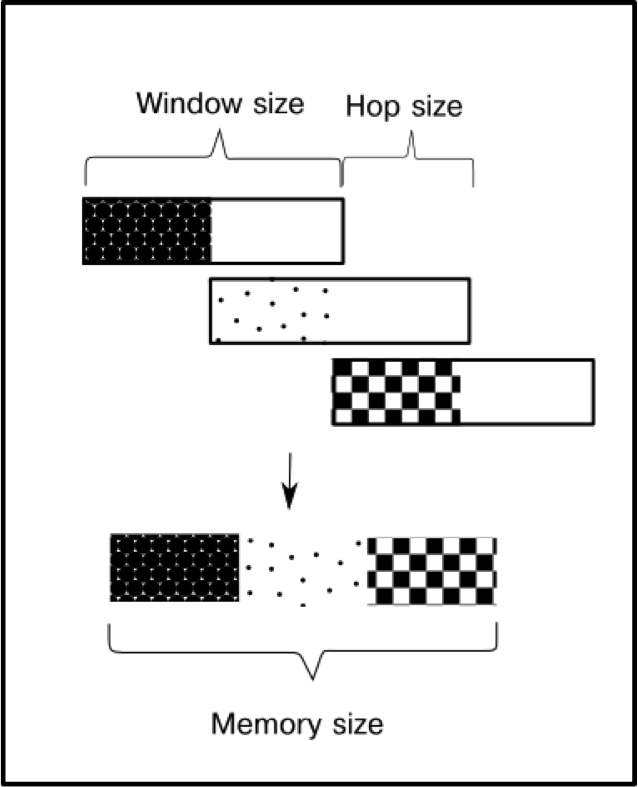
\includegraphics[width=90mm]{figures/dm_ws_hs_mem.png}
\caption{A graphical representation of window size, hop size and
  memory size in the Audio Feature Extraction algorithm that has been
  used.}
\label{fig:dm_ws_hs_mem}
\end{figure}

%
% MFCC Features
%

- MFCC features are derived from a power spectrum of the features,
which takes as parameters the window size and hop size.
- Another parameter is the number of windows over which to take the
mean and standard deviation of the MFCC coefficients.
- We did a parameter scan over these quantities to find the optimal
values for these parameters

\begin{table}
\begin{tabular}{|l|l|l|l|l|}
\hline
Feature options & Extract Time & Train Time & Predict time & Percent Correct \\

--mfcc -ws 256  -hp 128  -m 1   &  535.01 & 133.01 & 26.75 &  74.1081 \\
--mfcc -ws 512  -hp 256  -m 1   &  310.93 &  76.18 & 13.29 &  72.8382 \\
--mfcc -ws 1024 -hp 512  -m 1   &  271.87 &  28.92 &  6.91 &  72.497 \\
--mfcc -ws 2048 -hp 1024 -m 1   &  216.90 &  12.36 &  3.26 &  72.6641 \\
--mfcc -ws 4096 -hp 2048 -m 1   &  267.31 &   6.52 &  1.69 &  71.8926 \\
--mfcc -ws 8192 -hp 4096 -m 1   &  233.09 &   2.55 &  0.82 &  72.8763 \\
--mfcc -ws 256  -hp 128  -m 2   &  490.53 & 551.92 & 45.32 &  74.301 \\
--mfcc -ws 512  -hp 256  -m 2   &  382.02 & 265.41 & 22.50 &  74.2827 \\
--mfcc -ws 1024 -hp 512  -m 2   &  300.11 & 127.21 & 11.38 &  74.1882 \\
--mfcc -ws 2048 -hp 1024 -m 2   &  197.15 &  54.96 &  5.66 &  74.5691 \\
--mfcc -ws 4096 -hp 2048 -m 2   &  233.10 &  25.78 &  2.89 &  75.1136 \\
--mfcc -ws 8192 -hp 4096 -m 2   &  187.92 &  11.75 &  1.47 &  75.9031 \\
--mfcc -ws 256  -hp 128  -m 5   &  506.67 & 420.02 & 45.23 &  74.8874 \\
--mfcc -ws 512  -hp 256  -m 5   &  283.64 & 218.19 & 22.56 &  74.4823 \\
--mfcc -ws 1024 -hp 512  -m 5   &  320.14 & 106.52 & 11.37 &  74.6717 \\
--mfcc -ws 2048 -hp 1024 -m 5   &  231.64 &  49.37 &  5.68 &  75.5929 \\
--mfcc -ws 4096 -hp 2048 -m 5   &  158.95 &  22.53 &  2.89 &  76.7524 \\
--mfcc -ws 8192 -hp 4096 -m 5   &  253.30 &  11.88 &  1.49 &  78.2226 \\
--mfcc -ws 256  -hp 128  -m 10  &  539.47 & 389.21 & 45.01 &  75.1089 \\
--mfcc -ws 512  -hp 256  -m 10  &  248.18 & 202.71 & 22.51 &  74.742 \\
--mfcc -ws 1024 -hp 512  -m 10  &  228.71 & 108.72 & 11.34 &  75.4495 \\
--mfcc -ws 2048 -hp 1024 -m 10  &  238.44 &  46.47 &  5.67 &  76.7604 \\
--mfcc -ws 4096 -hp 2048 -m 10  &  193.98 &  22.66 &  2.91 &  78.894 \\
--mfcc -ws 8192 -hp 4096 -m 10  &  217.53 &  11.04 &  1.50 &  81.507 \\
--mfcc -ws 256  -hp 128  -m 20  &  524.22 & 415.89 & 45.40 &  75.3 \\
--mfcc -ws 512  -hp 256  -m 20  &  273.18 & 225.25 & 22.55 &  75.4575 \\
--mfcc -ws 1024 -hp 512  -m 20  &  277.19 & 121.40 & 11.55 &  76.7566 \\
--mfcc -ws 2048 -hp 1024 -m 20  &  279.67 &  52.01 &  5.77 &  78.836 \\
--mfcc -ws 4096 -hp 2048 -m 20  &  272.74 &  21.76 &  2.87 &  81.9996 \\
--mfcc -ws 8192 -hp 4096 -m 20  &  157.45 &  10.38 &  1.48 &  86.1934 \\
--mfcc -ws 256  -hp 128  -m 40  &  522.67 & 500.58 & 45.35 &  75.9696 \\
--mfcc -ws 512  -hp 256  -m 40  &  330.21 & 240.39 & 22.46 &  76.6192 \\
--mfcc -ws 1024 -hp 512  -m 40  &  212.77 & 116.80 & 11.28 &  78.7194 \\
--mfcc -ws 2048 -hp 1024 -m 40  &  230.12 &  54.62 &  5.73 &  82.1643 \\
--mfcc -ws 4096 -hp 2048 -m 40  &  251.88 &  20.76 &  2.90 &  86.7257 \\
--mfcc -ws 8192 -hp 4096 -m 40  &  221.18 &   7.73 &  1.46 &  94.2099 \\
--mfcc -ws 256  -hp 128  -m 80  &  486.19 & 579.59 & 44.88 &  77.2021 \\
--mfcc -ws 512  -hp 256  -m 80  &  360.64 & 261.26 & 23.12 &  78.6088 \\
--mfcc -ws 1024 -hp 512  -m 80  &  299.42 & 118.50 & 11.25 &  81.9441 \\
--mfcc -ws 2048 -hp 1024 -m 80  &  206.75 &  45.72 &  5.65 &  87.1649 \\
--mfcc -ws 4096 -hp 2048 -m 80  &  219.33 &  17.61 &  3.21 &  94.357 \\
--mfcc -ws 8192 -hp 4096 -m 80  &  193.94 &   5.73 &  1.66 &  97.8014 \\
--mfcc -ws 256  -hp 128  -m 160 &  546.38 & 649.18 & 51.00 &  79.4754 \\
--mfcc -ws 512  -hp 256  -m 160 &  315.60 & 268.16 & 25.44 &  81.7902 \\
--mfcc -ws 1024 -hp 512  -m 160 &  264.84 & 116.40 & 12.75 &  87.1799 \\
--mfcc -ws 2048 -hp 1024 -m 160 &  218.20 &  36.06 &  5.75 &  94.1804 \\
--mfcc -ws 4096 -hp 2048 -m 160 &  157.51 &  10.70 &  2.87 &  97.8546 \\
--mfcc -ws 8192 -hp 4096 -m 160 &  163.09 &   3.65 &  1.47 &  99.0869 \\

\hline


\hline
\end{tabular}
\caption{Table of MFCC results with different window sizes - liblinear}
\label{table:obv-1-mfcc}
\end{table}


%
% Different numbers of MFCCs
%

- You can also change the number of MFCCs, 13 is a typical number, 20
is also used.
- Dolphins (and presumably orcas) have about the same number of inner
hair cells but have 3 times as many gangilon cells.  (How would this
affect things?)


\begin{table}
\begin{tabular}{|l|l|l|l|l|l|l|l|l|}
\hline

winSize         & hopSize         & memory          & numMfccs        & total vectors   & feature time    & train time      & predict time    & accuracy        \\
20              & 512             & 256             & 5               & 5169            & 0.96            & 2.93            & 0.04            & 78.93           \\
20              & 512             & 256             & 13              & 5169            & 1.08            & 3.97            & 0.08            & 94.00           \\
20              & 512             & 256             & 20              & 5169            & 1.23            & 4.73            & 0.12            & 96.92           \\
20              & 512             & 256             & 40              & 5169            & 1.77            & 6.78            & 0.23            & 97.60           \\
20              & 512             & 256             & 60              & 5169            & 1.90            & 9.59            & 0.34            & 97.91           \\

\hline
\end{tabular}
\caption{Table of MFCC results with different window sizes - liblinear}
\label{table:obv-2-numMfcc}
\end{table}

%
% Liblinear parameters
%

- Liblinear has different parameters that can be used.  We did a
parameter scan of these parameters

\begin{table}
\begin{tabular}{|l|l|l|l|l|l|}
\hline

type of solver                                                    & s               &c               & train time      & predict time    & accuracy        \\
L2-regularized L2-loss support vector classification (dual)       & 1               & 0.00            & 0.26            & 0.08            & 93.85           \\
L2-regularized L2-loss support vector classification (dual)       & 1               & 1.00            & 3.92            & 0.08            & 94.00           \\
L2-regularized L2-loss support vector classification (dual)       & 1               & 1000.00         & 4.51            & 0.09            & 93.27           \\
L2-regularized L2-loss support vector classification (dual)       & 1               & 1.00            & 4.69            & 0.08            & 94.00           \\
L2-regularized L2-loss support vector classification (primal)     & 2               & 1.00            & 0.20            & 0.08            & 95.12           \\
L2-regularized L1-loss support vector classification (dual)       & 3               & 1.00            & 4.09            & 0.08            & 92.78           \\
support vector classification by Crammer and Singer               & 4               & 1.00            & 32.68           & 0.08            & 96.05           \\
L1-regularized L2-loss support vector classification              & 5               & 1.00            & 0.73            & 0.08            & 95.67           \\
L1-regularized logistic regression                                & 6               & 1.00            & 0.62            & 0.09            & 95.65           \\
L2-regularized logistic regression (dual)                         & 7               & 1.00            & 9.64            & 0.08            & 95.57           \\



\hline
\end{tabular}
\caption{Table of liblinear parameters}
\label{table:obv-3-liblinearParams}
\end{table}

- From this we can see the best classification performance was from the xxx solver 
- The fastest time was for the xxx solver, and gave a performance of xxx\%

%
% Different features
%

- We then did a test to see if adding other features helped the
classification using the window size, hop size and memory from the
last experiment.
- We added spectral features including Centroid, Rolloff, and Flux
- Description of Centroid, Rolloff, Flux, Kurtosis
- Added Linear Prediction Coefficients
- LPCC - Convert LPC coefficients to Cepstrum coefficients.
- LSP - Linear Spectral Pair
- Spectral Crest Factor
- Spectral Flatness Measure 
- Zero crossings
- Added pitch detector - Yin
- Added Chroma

\begin{table}
\begin{tabular}{|l|l|l|l|l|}
\hline
Features & Percent Correct \\
\hline


options                                                                          & feature time    &train time      & predict time    & accuracy        \\
--mfcc                                                                           & 1.23            & 0.27            & 0.12            & 96.05           \\
--ctd                                                                            & 2.95            & 0.02            & 0.01            & 33.33           \\
--rlf                                                                            & 2.85            & 0.02            & 0.01            & 33.33           \\
--flx                                                                            & 2.78            & 0.02            & 0.01            & 33.33           \\
--kurtosis                                                                       & 0.86            & 0.02            & 0.01            & 37.22           \\
--skewness                                                                       & 1.35            & 0.02            & 0.01            & 31.98           \\
--sfm                                                                            & 1.42            & 0.26            & 0.13            & 93.25           \\
--scf                                                                            & 1.22            & 0.34            & 0.14            & 91.76           \\
--chroma                                                                         & 1.25            & 0.20            & 0.09            & 67.52           \\
--rms                                                                            & 0.74            & 0.02            & 0.01            & 33.00           \\
--yin                                                                            & 2.01            & 0.02            & 0.01            & 32.77           \\
--mfcc --ctd --rlf --flx                                                         & 1.23            & 0.28            & 0.12            & 96.05           \\
--mfcc --ctd --rlf --flx --kurtosis --skewness --sfm --scf                       & 3.49            & 0.95            & 0.40            & 97.41           \\
--mfcc --ctd --rlf --flx --kurtosis --skewness --sfm --scf --chroma              & 3.26            & 1.65            & 0.48            & 97.14           \\
--mfcc --ctd --rlf --flx --kurtosis --skewness --sfm --scf --chroma --yin        & 4.60            & 1.76            & 0.49            & 95.53           \\
--mfcc --ctd --rlf --flx --kurtosis --skewness --sfm --scf --chroma --yin --rms  & 4.63            & 1.82            & 0.49            & 95.49           \\


\hline
\end{tabular}
\caption{Table of MFCC + Spectral Descriptors with different window
  sizes - liblinear}
\label{table:obv-4-differentFeatures}
\end{table}

%
% Spectrogram image
%

Spectrogram image



\begin{table}
\begin{tabular}{|l|l|l|l|l|}
\hline


\hline
\end{tabular}
\caption{}
\label{table:obv-5-spectrogramImage}
\end{table}




%
% Stabilized auditory image
%

Another type of feature that could be used for call detection is the
Stablised Auditory Image.  

- Brief description of SAI
- Diagram of SAI generation

- Different filterbanks to use - Gammatone, PZFC, CARFAC.  These are
all progressively more detailed models of the cochlea, and model both
the filtering processes within the cochlea as well as the automatic
gain control mechanism in the mechanical cochlea.

The filterbank is followed by a halfwave linear rectification
algorithm which models the way that inner hair cells communicate with
neurons.  In this process, there is a electochemical gradient between
the two sides of membrane the inner hair cell is attached to, and when
the inner hair cell flexes in the forward direction, it physically
opens a channel that allows ions to pass, and when it flexes in the
reverse direction, this channel closes.  This gives a signal that is
similar to a half-wave rectified filter, in which only the positive
part of the signal is transmitted, and the negative part is made zero.

This is followed by a strobe detector, which looks for a local maximum
in the signal, and when a certain threshold has been detected, it
sends the signal to the next stage in the pipeline.  This local
maximum has a decaying threshold with a timeout, so that strobes are
guaranteed to be delivered at a certain rate, even if the signal is at
a low value.


- Different 
- Gives clear patterns on image when audio with a pulsed nature is
  used as input
- Show frames of SAI movie showing the different sections of audio and
  how well they work




\begin{table}
\begin{tabular}{|l|l|l|}
\hline


\hline
\end{tabular}
\caption{}
\label{table:obv-6-SAI}
\end{table}




%
% Downsampling
%


- Then took the best set of these features 
- The full features are too expensive to use with Weka, too many
feature vectors
- Downsample the features to obtain a smaller set to test with
different classifiers


\begin{table}
\begin{tabular}{|l|l|l|l|l|}
\hline
ds              & feature time    &train time      & predict time    & accuracy        \\
\hline
1               & 1.23            & 0.27            & 0.12            & 96.05           \\
2               & 0.98            & 0.14            & 0.06            & 95.98           \\
5               & 0.80            & 0.06            & 0.03            & 96.03           \\
10              & 0.76            & 0.03            & 0.01            & 95.74           \\
20              & 0.73            & 0.02            & 0.01            & 96.14           \\
50              & 0.70            & 0.01            & 0.01            & 97.12           \\
100             & 0.69            & 0.01            & 0.00            & 100.00          \\
200             & 0.70            & 0.01            & 0.00            & 100.00          \\
500             & 0.68            & 0.00            & 0.00            & 100.00          \\
1000            & 0.68            & 0.00            & 0.00            & 100.00          \\


\hline
\end{tabular}
\caption{Table of downsampling with MFCC + Spectral with different
  downsampling rates with liblinear}
\label{table:obv-7-downsampling}
\end{table}

- From this we can see that we start to get a decrease in performance
of the classifier at a downsampling ratio of xxx
- This helps the predictor by needing to output less data

%
% libsvm linear kernel
%

With the reduced set of features, we can now test SVM using different
kernels, which is supported in libsvm.  The first one we test is the
linear kernel, which should be identical to liblinear:


\begin{table}
\begin{tabular}{|l|l|l|l|l|l|l|}
\hline

s               & t               & c               & gamma           & train time      & predict time    & accuracy        \\
0               & 0               & 0.0010          & 1.0000          & 0.29            & 0.21            & 57.35           \\
0               & 0               & 0.0100          & 1.0000          & 0.19            & 0.16            & 91.88           \\
0               & 0               & 0.1000          & 1.0000          & 0.10            & 0.09            & 95.45           \\
0               & 0               & 1.0000          & 1.0000          & 0.08            & 0.06            & 97.68           \\
0               & 0               & 10.0000         & 1.0000          & 0.10            & 0.05            & 98.84           \\
0               & 0               & 100.0000        & 1.0000          & 0.12            & 0.05            & 99.52           \\
0               & 0               & 1000.0000       & 1.0000          & 0.54            & 0.04            & 99.61           \\
0               & 0               & 10000.0000      & 1.0000          & 0.44            & 0.04            & 100.00          \\
0               & 0               & 100000.0000     & 1.0000          & 0.44            & 0.04            & 100.00          \\


\hline
\end{tabular}
\caption{Linear kernel for libsvm}
\label{table:obv-6-libsvm-linear}
\end{table}

%
% libsvm polynomial kernel
%

We now test with the polynomial kernel, which has a kernel of the form
$(gamma*u'*v + coef0)^degree$

For this experiment, we test different numbers of degrees and different values of gamma and C.

\begin{table}
\begin{tabular}{|l|l|l|l|l|l|l|l|}
\hline

s               & t               & c               & gamma           & degree          & train time      & predict time    & accuracy        \\
0               & 1               & 1000.0000       & 1.0000          & 1               & 0.46            & 0.04            & 99.61           \\
0               & 1               & 1000.0000       & 1.0000          & 2               & 0.08            & 0.05            & 100.00          \\
0               & 1               & 1000.0000       & 1.0000          & 3               & 0.09            & 0.06            & 100.00          \\
0               & 1               & 1000.0000       & 1.0000          & 5               & 0.09            & 0.07            & 100.00          \\
0               & 1               & 1000.0000       & 1.0000          & 10              & 0.12            & 0.08            & 100.00          \\
0               & 1               & 1000.0000       & 1.0000          & 20              & 0.16            & 0.09            & 100.00          \\
0               & 1               & 0.0010          & 1.0000          & 5               & 0.09            & 0.07            & 99.71           \\
0               & 1               & 0.0100          & 1.0000          & 5               & 0.09            & 0.07            & 100.00          \\
0               & 1               & 0.1000          & 1.0000          & 5               & 0.10            & 0.07            & 100.00          \\
0               & 1               & 1.0000          & 1.0000          & 5               & 0.10            & 0.07            & 100.00          \\
0               & 1               & 10.0000         & 1.0000          & 5               & 0.10            & 0.07            & 100.00          \\
0               & 1               & 100.0000        & 1.0000          & 5               & 0.10            & 0.07            & 100.00          \\
0               & 1               & 1000.0000       & 1.0000          & 5               & 0.10            & 0.07            & 100.00          \\
0               & 1               & 10000.0000      & 1.0000          & 5               & 0.09            & 0.07            & 100.00          \\
0               & 1               & 100000.0000     & 1.0000          & 5               & 0.10            & 0.07            & 100.00          \\
0               & 1               & 1.0000          & 0.0010          & 5               & 0.36            & 0.24            & 33.46           \\
0               & 1               & 1.0000          & 0.0100          & 5               & 0.35            & 0.22            & 33.46           \\
0               & 1               & 1.0000          & 0.1000          & 5               & 0.16            & 0.12            & 92.46           \\
0               & 1               & 1.0000          & 1.0000          & 5               & 0.10            & 0.07            & 100.00          \\
0               & 1               & 1.0000          & 10.0000         & 5               & 0.09            & 0.07            & 100.00          \\
0               & 1               & 1.0000          & 100.0000        & 5               & 0.09            & 0.07            & 100.00          \\
0               & 1               & 1.0000          & 1000.0000       & 5               & 0.09            & 0.08            & 100.00          \\
0               & 1               & 1.0000          & 10000.0000      & 5               & 0.11            & 0.07            & 100.00          \\
0               & 1               & 1.0000          & 100000.0000     & 5               & 0.09            & 0.07            & 100.00          \\

\hline
\end{tabular}
\caption{Linear kernel for libsvm}
\label{table:obv-6-libsvm-linear}
\end{table}

From this we see that xxxx


%
% libsvm sigmoid kernel
%

The sigmoid kernel is of interest because it is of a similar form to
the linear perceptron used in neural networks, a classifier that we
will also investigate.  The form of the sigmoid kernel is tanh(gamma*u'*v + coef0)

The parameters for the sigmoid kernel are c and gamma.  We did a
parameter search of these parameters.

\begin{table}
\begin{tabular}{|l|l|l|l|l|l|l|}
\hline

s               & t               & c               & gamma           & train time      & predict time    & accuracy        \\
0               & 3               & 0.0010          & 1.0000          & 0.51            & 0.34            & 33.46           \\
0               & 3               & 0.0100          & 1.0000          & 0.47            & 0.33            & 35.88           \\
0               & 3               & 0.1000          & 1.0000          & 0.44            & 0.37            & 51.35           \\
0               & 3               & 1.0000          & 1.0000          & 0.37            & 0.31            & 38.30           \\
0               & 3               & 10.0000         & 1.0000          & 0.29            & 0.25            & 35.69           \\
0               & 3               & 100.0000        & 1.0000          & 0.27            & 0.23            & 35.59           \\
0               & 3               & 1000.0000       & 1.0000          & 0.27            & 0.22            & 35.49           \\
0               & 3               & 10000.0000      & 1.0000          & 0.28            & 0.23            & 35.49           \\
0               & 3               & 100000.0000     & 1.0000          & 0.27            & 0.22            & 35.49           \\
0               & 3               & 1.0000          & 0.0010          & 0.48            & 0.35            & 57.35           \\
0               & 3               & 1.0000          & 0.0100          & 0.32            & 0.26            & 91.78           \\
0               & 3               & 1.0000          & 0.1000          & 0.16            & 0.14            & 93.52           \\
0               & 3               & 1.0000          & 1.0000          & 0.36            & 0.30            & 38.30           \\
0               & 3               & 1.0000          & 10.0000         & 0.30            & 0.22            & 37.62           \\
0               & 3               & 1.0000          & 100.0000        & 0.26            & 0.21            & 36.36           \\
0               & 3               & 1.0000          & 1000.0000       & 0.27            & 0.20            & 36.36           \\
0               & 3               & 1.0000          & 10000.0000      & 0.26            & 0.21            & 36.36           \\
0               & 3               & 1.0000          & 100000.0000     & 0.27            & 0.21            & 36.36           \\



\hline
\end{tabular}
\caption{Linear kernel for libsvm}
\label{table:obv-6-libsvm-linear}
\end{table}

From this we see that the performance was lower than the RBF kernel,
but with suitable parameters of C and gamma we were able to obtain
adequate classification performance.

%
% libsvm RBF  kernel
%

We then tested a very commonly used kernel, the Radial Basis Function kernel.  
- Brief description of RBF kernel
- This gives an infinite dimension hyperplane
- The form of the RBF kernel is $exp(-gamma*|u-v|^2)$
- The two parameters to vary for the RBF kernel are C and gamma

\begin{table}
\begin{tabular}{|l|l|l||l|l|l|l|}
\hline

s               & t               & c               & gamma           & train time      & predict time    & accuracy        \\
0               & 2               & 0.0010          & 1.0000          & 0.47            & 0.31            & 33.46           \\
0               & 2               & 0.0100          & 1.0000          & 0.41            & 0.31            & 33.46           \\
0               & 2               & 0.1000          & 1.0000          & 0.37            & 0.32            & 96.42           \\
0               & 2               & 1.0000          & 1.0000          & 0.39            & 0.21            & 99.81           \\
0               & 2               & 10.0000         & 1.0000          & 0.39            & 0.22            & 100.00          \\
0               & 2               & 100.0000        & 1.0000          & 0.38            & 0.35            & 100.00          \\
0               & 2               & 1000.0000       & 1.0000          & 0.38            & 0.20            & 100.00          \\
0               & 2               & 10000.0000      & 1.0000          & 0.38            & 0.20            & 100.00          \\
0               & 2               & 100000.0000     & 1.0000          & 0.38            & 0.21            & 100.00          \\
0               & 2               & 1.0000          & 0.0010          & 0.40            & 0.30            & 85.88           \\
0               & 2               & 1.0000          & 0.0100          & 0.22            & 0.32            & 93.62           \\
0               & 2               & 1.0000          & 0.1000          & 0.12            & 0.13            & 97.29           \\
0               & 2               & 1.0000          & 1.0000          & 0.38            & 0.20            & 99.81           \\
0               & 2               & 1.0000          & 10.0000         & 0.57            & 0.30            & 100.00          \\
0               & 2               & 1.0000          & 100.0000        & 0.57            & 0.30            & 100.00          \\
0               & 2               & 1.0000          & 1000.0000       & 0.36            & 0.24            & 100.00          \\
0               & 2               & 1.0000          & 10000.0000      & 0.36            & 0.24            & 100.00          \\
0               & 2               & 1.0000          & 100000.0000     & 0.37            & 0.24            & 100.00          \\


\hline
\end{tabular}
\caption{RBF kernel for libsvm}
\label{table:obv-8-libsvm-rbf}
\end{table}

From this we see that we got the best classification with the RBF
kernel.  However, the performance was not significantly greater than
that of the linear classifier, and by using the linear classifier we
are able to 



%
% Logistic regression
%

Logistic Regression

- Type of linear regression analysis
- Classifies instances based on a logistic function
- Interesting to look at because it is widely used, but also because
  there exist algorithms to distribute it on a large cluster of
  machines using a map-reduce paradigm.  This could give it the
  ability to use very large training datasets efficiently

The multinomial log-likelihood is:

$L = -sum[i=1..n]{ sum[j=1..(k-1)](Yij * ln(Pj(Xi))) + (1 - (sum[j=1..(k-1)]Yij)) * ln(1 - sum[j=1..(k-1)]Pj(Xi)) } + ridge * (B^2)$

le Cessie, S. and van Houwelingen, J.C. (1992). Ridge Estimators in Logistic Regression. Applied Statistics, Vol. 41, No. 1, pp. 191-201.

\begin{table}
\begin{tabular}{|l|l|l|}
\hline

wekaOptions          & weka time       &accuracy        \\
-R 1.0E-8            & 13.29           & 87.31           \\
-R 1.0               & 15.16           & 87.46           \\
-R 10.0              & 13.72           & 87.33           \\
-R 100.0             & 14.57           & 86.40           \\
-R 1000.0            & 10.25           & 83.69           \\
-R 10000.0           & 6.64            & 79.18           \\

\hline
\end{tabular}
\caption{Table showing results of Logistic Regression classifier with
  different values of xxxx}
\label{table:obv-10-logistic}
\end{table}

From this we can see that the Logistic Regression classifier xxxx.


%
% Naive Bayes
%
Naive Bayes

- Bayes theorem P(X|Y) = P(X)P(Y|X)/P(Y)
- Description of Bayes theorem
- Uses Maximum Likelihood

- Naive Bayes uses Bayes theorem for classification, and assumes that
all attributes are independent.  Even though in many classification problems
features are not independent of each other, in many cases this simple model works well.

- One advantage of Naive Bayes is that it can be trained efficiently.

George H. John and Pat Langley (1995). Estimating Continuous
Distributions in Bayesian Classifiers. Proceedings of the Eleventh
Conference on Uncertainty in Artificial
Intelligence. pp. 338-345. Morgan Kaufmann, San Mateo.


\begin{table}
\begin{tabular}{|l|l|l|}
\hline

wekaOptions          & weka time       &accuracy        \\
                     & 2.35            & 87.12           \\
-D                   & 4.45            & 88.31           \\
-K                   & 121.14          & 88.82           \\


\hline
\end{tabular}
\caption{Table showing results of Naive Bayes classifier with
  different values of xxxx}
\label{table:obv-11-naiveBayes}
\end{table}

From these results we can see that xxxx.

%
% J48 - C4.5
%

J48 - C4.5

Decision tree based method

Developed in 1993 by Quinlan \cite{quinlan93}

Similar to the ID3 (Iterative Dichotomiser 3) algorithm \cite{quinlan86}

Constructs a tree that makes the optimal decision based on information
entropy at each leaf

Starts with all the original data points in one set.

At each step it iterates over each leaf of the tree, and looks at the
set of instances at that leaf.  It goes through all the attributes of
that set and finds the attribute that can give the highest information
gain (or lowest information entropy) if we were to split the leaf
based on that attribute.  It then splits that leaf by making a new
decision at that leaf splitting the set S into two sets using that
attribute.  This process is iterated over all the leaves until either
each element in that leaf has the same label, there are no more
attributes to be selected, or there are no more examples in the subset
at this leaf.

Advantage is that it is very quick to predict values given a trained
classifier



\begin{table}
\begin{tabular}{|l|l|l|}
\hline

wekaOptions          & weka time       &accuracy        \\
                     & 21.86           & 89.88           \\
-U                   & 15.04           & 89.79           \\
-R                   & 11.40           & 89.75           \\
-S                   & 15.34           & 89.90           \\
-L                   & 13.38           & 89.88           \\
-A                   & 12.96           & 89.88           \\
-C 0.01              & 12.66           & 90.06           \\
-C 0.1               & 12.85           & 90.00           \\
-C 0.5               & 12.96           & 89.82           \\
-C 0.9               & 13.75           & 89.79           \\
-M 3                 & 12.87           & 89.77           \\
-M 5                 & 12.41           & 89.86           \\
-M 10                & 11.85           & 89.73           \\



\hline
\end{tabular}
\caption{Table showing results of J48 C4.5 classifier with
  different values of xxxx}
\label{table:obv-12-j48}
\end{table}

From these results we can see xxxx.


%
% Random Forest
%

Random Forest - Class for constructing random forests. 

The Random Forest model of classification also uses decision trees as
described above with the C4.5 classifier, but constructs many
different trees using a subset of the features and uses the output of
each tree as a vote in the final classification, choosing the label
with the most votes.  It was originally developed by Breiman and
Cutler \cite{breiman2001}, and uses ideas from bagging, or bootstrap
aggregating, where multiple sets of new training sets are generated
from an original training set by sampling uniformly from the original
training set with replacement.

The algorithm has the advantage that not all the features have to be
used in the construction of each new tree like in the C4.5 algorithm,
which can give speed benefits, which is somewhat offset by the need to
train multiple trees.  By choosing random features xxxx.



Leo Breiman. Random Forests. Machine Learning 45 (1):5-32, October 2001.


\begin{table}
\begin{tabular}{|l|l|l|}
\hline

wekaOptions          & weka time       &accuracy        \\
-K 1                 & 8.32            & 88.72           \\
-K 2                 & 11.48           & 91.89           \\
-K 3                 & 14.41           & 93.17           \\
-K 4                 & 17.75           & 93.77           \\
-K 5                 & 21.53           & 94.12           \\
-K 7                 & 27.92           & 94.41           \\
-K 10                & 37.24           & 94.12           \\
-K 20                & 71.73           & 94.08           \\
-I 1                 & 2.83            & 86.23           \\
-I 2                 & 4.83            & 87.54           \\
-I 3                 & 6.79            & 91.64           \\
-I 4                 & 9.18            & 92.13           \\
-I 5                 & 11.46           & 93.13           \\
-I 7                 & 15.08           & 93.89           \\
-I 10                & 21.41           & 94.12           \\
-I 20                & 42.30           & 94.66           \\
-I 50                & 102.75          & 95.01           \\


\hline
\end{tabular}
\caption{Table showing results of random forest classifier with
  different values of xxxx}
\label{table:obv-13-randomForest}
\end{table}

%
% Multilayer Perceptron
%

- MultilayerPerceptron - A neural network classifier that uses
backpropogation to train the algorithm.  All nodes use a sigmoid
function.
- Deep belief network 

- Has a number of parameters that can be set:

Number of hidden layers H, which is the number of layers of neurons
between the input and output layers.  By default in the Weka
implementation it is set as (attribs + classes) / 2, which for the
MFCC data and the OBV classification task would be (25 + 3) / 2 = 14.
We did a parameter sweep from xxx to xxx for this variable.

Another variable is the learning rate for the backpropogation
algorithm ...

Another variable is the momentum rate for the backpropogation
algorithm ...

\begin{table}
\begin{tabular}{|l|l|l|}
\hline

wekaOptions          & weka time       &accuracy        \\
-N 5                 & 6.60            & 90.73           \\
-H 0 -N 5            & 2.76            & 87.62           \\
-M 0.01 -N 5         & 6.58            & 90.25           \\
-M 0.7 -N 5          & 6.71            & 93.29           \\
-L 0.01 -N 5         & 6.82            & 67.92           \\
-L 0.7 -N 5          & 6.58            & 93.13           \\


\hline
\end{tabular}
\caption{Table showing results of multilayer perceptron classifier with
  different values of xxxx}
\label{table:obv-14-multilayerPerceptron}
\end{table}






%
% Deep Belief Network
%

\subsection{Deep Belief Network}


- description of Deep Belief Networks

\begin{table}
\begin{tabular}{|l|l|l|l|l|}
\hline
Window Size & Hop Size & Memory & Total feature vectors & Percent Correct \\
\hline


\hline
\end{tabular}
\caption{Table of downsampling 100 (or whatever is reasonable) with weka with
MFCC + Spectral with different}
\label{table:mfccSpectralWeka}
\end{table}



\section{Call classification}

Once the large amount of data has been segmented into sections that
have been identified as orca calls, we are now interested in
classifying these calls based on the call catalog of Ford
\cite{ford87}.  As an additional and related task, we are also
interested in classifying these calls based on the clan, pod, subpod
and matriline that made the calls.  These are overlapping tasks as
some calls are only made by one pod so classifying some of them would
automatically give the pod they came from, like the N47 call.  Other
calls are very distinct from pod to pod, and can be handled as
seperate classification tasks, and others are so similar, like N3,
that it is difficult for an untrained person to differentiate between
calls made by different pods, and would likely be a difficult machine
learning task.

It should be noted though that there are other forms of information
that can be used by scientists in the future when using classifiers
from this work, the most important being direct visual observation
combined with the use of the photo identification catalog.  This could
be combined with acoustic arrays of hydrophones to localize individual
whales.



%
% Spectrogram cross-correlation
%


Another method that is used for call detection is spectrogram
cross-correlation, where a kernel is used to

- Description of Spectrogram Cross-correlation
- Take spectrograms of call catalog as kernels
- Run each kernel over the spectrogram


\begin{table}
\begin{tabular}{|l|l|l|l|l|}
\hline
Window Size & Hop Size & Memory & Total feature vectors & Percent Correct \\
\hline


\hline
\end{tabular}
\caption{Table of downsampling 100 (or whatever is reasonable) with weka with
MFCC + Spectral with different}
\label{table:mfccSpectralWeka}
\end{table}





%
% Voting
%

The previous experiments were on a feature by feature basis.  The
pulsed calls made by orcas extend over a span of time, typically from
0.5 to 3 seconds in length, and we can take advantage of this fact by
using a window in which the classifications of individual feature
vectors can be combined using a voting paradigm.  In this experiment,
all the orca, background and voice clips were concatenated together
in order to approximate the continuous nature of the actual sounds to
be classified.

\begin{table}
\begin{tabular}{|l|l|l|}
\hline
\# of frames & Percent Correct \\
\hline


\hline
\end{tabular}
\caption{Table of spectral features with voting per slice}
\label{table:obvVoting}
\end{table}


%
% Image compression
%

\subsection{Image compression}


- Description of Image compression to find calls
- Use call catalog as kernels
- Spectrogram used as 

\begin{table}
\begin{tabular}{|l|l|l|l|l|}
\hline
Window Size & Hop Size & Memory & Total feature vectors & Percent Correct \\
\hline


\hline
\end{tabular}
\caption{Table of downsampling 100 (or whatever is reasonable) with weka with
MFCC + Spectral with different}
\label{table:mfccSpectralWeka}
\end{table}


%
% Dynamic Time Warping
%

\subsection{Dynamic Time Warping}


- Description of Dynamic Time Warping (DTW)
- Similar to spectrogram cross-correlation but also takes into account
  time differences
- Expensive for doing call detection


\begin{table}
\begin{tabular}{|l|l|l|}
\hline

\hline


\hline
\end{tabular}
\caption{SBI}
\label{table:obvSBI}
\end{table}

%
% Standard MIR features
%




%
% Spectrogram cross correlation
%





%
% Image compression
%





%
% Dynamic Time warping
%




%
% Vector quantization and SAX/bioinformatics
%





%
% Stabilized auditory images
%





%
% Deep belief networks on spectrograms
%









\section{Distributed Computation}




\subsection{Grid Computing}

\subsection{Mahout}



%
% Expert Interface
%

\section{Expert Interface}

It is vitally important to evaluate the system that we have created
with the actual researchers who will be using this system.  One could
imagine using a variety of methods to evaluate this system, including
Laboratory Experiments, Sample Surveys and Field Study.

We have completed a very small Ethnographic based Field Study in which
several cetacean biologists made annotations using the Orchive
interface.  In this study, we observed 5 different scientists of
varying levels of expertise, two of these were researchers with over
40 years of experience with orca vocalizations, one was a
post-graduate researcher who had done her Ph.D. studying orca
vocalizations, one was a M.Sc. student who had not studied orca
vocalizations before, but had studied pilot whales, and one was an
undergraduate student who had extensive experience with visually
observing whales.

The results from this field study were very interesting and
encouraging.  One of the respondents said:

``I wish I had this when I was doing my Ph.D.  It would have made my
research much easier''

another said:

``This makes it possible to finally access all this data easily.''

When shown the predictions from machine learning, one of the
researchers became quite excited and said:

``Wow!  It can tell the difference between the different calls!''

One respondent had concerns that she would not know if the people who
were making the annotations would really know what they were doing.
This same sentiment was shared by most of the other respondents.
Another discussion ensued about inter-observer reliability, the quality
of annotations, and to know who had made which annotation, this
highlighted the importance for reputation management systems to be
implemented in this application.

Another topic that the subjects talked about was the importance for
being able to temporarily hide data that would be used in an upcoming
paper, so that other researchers would not be able to scoop them in
the race to publication in scholarly journals.  They said that:

``I want to share data with people in my lab, but not with people in
other labs, at least until I publish''

Another comment that was made was:

``I want to be able to write my field notes and have them attached to
a recording, but also be able to see all of them at once''

We must note that our Field Study borders on Critical Theory, because
we are not just interested in studying these researchers, but in
actively providing them tools to help them in their research.  For
this reason, it is difficult to remain completely objective about this
research.  In our opinion, it would be useful to have independent
field studies carried out by dispassionate researchers.

However, the biggest lesson that was learned in this project was that
in large part it was very difficult to engage expert biologists in
using this interface.  Even after 5 years of having the interface
available, and having over 30 scientists signed up on the site, only
10 of these researchers used the site in any substantial way.  


%
% Citizen Science Interface
%


\section{Citizen Science Interface}

In order to collect data from participants, we designed a Javascript
based game that used a simple matching paradigm. In this matching
game, the participant was presented with the instructions that are
shown in Figure \ref{fig:orcagameInstructions} where the participant
is shown a query clip at the top of the screen, and was then asked to
pick which of a series of four clips was most similar to this clip.
Each clip was shown as a spectrographic representation of the sound,
and when the participant clicked on the clip, the corresponding sound
was played.  When the participant was satisified with their guess,
they were asked to click on the ``Select'' button, and were notified
if their guess was ``correct'' or not.  After 5 rounds, the user was
shown a screen that said ``congratulations'', and was presented with
an option to complete a short online user survey.  In either case if
the survey was completed or not, the user was asked if they wanted to
play more rounds of the game.  The full game interface is shown in
Figure \ref{fig:orcagame}.  

This game was designed to be the simplest possible game like interface
that would gather data for this project, last year we had written a
much more involved interface that had many more features, such as
multiple turns per level where the user was first presented with only
the sounds and was asked to guess the clip, then if they got it wrong
they were allowed to see the spectrogram for a brief period of time
and guess again, and finally were allowed to see the spectrogram.
This interface also had a running score counter, where the user would
get points for correct answers, and if they answered correctly with
fewer hints in a level, they were rewarded with a higher score.  This
interface also had ``achievements'' which were an in game reward given
for correctly identifying 10 calls of a specific type, for example the
``N01'' call.  Another form of reward given was that after a series of
levels were completed, the user was given a screen showing them some
information about orcas along with pictures of orcas.  We hope to add
these additional features back into the game at some point, but were
interested in the current work if the simplest possible game mechanic
was engaging for users.

For this study, we chose the clips used in the game by hand in order
to evaluate the performance of participants on different types of data
and with different difficulty levels, and were able to manually set
what a ``correct'' guess was.  This allowed us to measure the
performance of users on ground truth data.  However, in our production
system, the correctness of a guess would be determined by a machine
learning system, perhaps combined with previous responses of other
participants.

We recruited participants through a series of different online
methods.  The first method was to recruit users through a mailing list
for graduate students and teachers of the computer science department
at the University of Victoria.  We recruited 9 participants in this
manner, and gave them a short introduction to the Orchive project and
to the game interface.  We then sat with them for three levels of the
game, where a level corresponds to a single user classification event.
We then asked them to play for as long as they wanted, and measured
the length of time they played for.  The length of time varied
considerably between participants, and is summarized along with the
percent correct and the total number of classifications in Table
\ref{table:orcagameInPerson}.

From this table, we can see that there was considerable variation in
the length of time that different users played the game, from a low of
about 11 minutes, to a maximum of about 47 minutes, and with a large
standard deviation of about 11 minutes.  The amount of classifications
that they made also varied considerably, and was somewhat, but not
heavily correlated with the amount of time they played the game.  This
was because some of the users listened to the sounds multiple times
before making a selection, and others quickly went through the
levels.

The percent of correct classifications also varied considerably
between users, with an average of about 77\%, with a low of 60.71\%
and a high of 82.5\%.  Some levels were designed to considerably more
difficult than others, and in a number of cases respondants were asked
to differniate between the same call type but vocalized by different
matrilines, a task that even expert listeners can find challenging.
From this initial pilot study, several minor interface flaws were
identified and were fixed, including reducing the number of
instruction screens describing how to use the game from four to one.

\begin{table}
\begin{tabular}{|c|c|c|c|}
\hline
Participant ID & \# classifications & \% correct & length of time (h:m:s) \\
\hline
1              &    28      &       60.71   &       0:24:11 \\                 
2              &    33      &       81.82   &       0:15:53 \\
3              &    45      &       75.56   &       0:11:24 \\
4              &    88      &       68.18   &       0:29:35 \\
5              &    40      &       80.00   &       0:12:19 \\
6              &    40      &       82.50   &       0:28:42 \\
7              &    71      &       78.87   &       0:47:18 \\
8              &    50      &       78.00   &       0:28:47 \\
9              &    43      &       86.05   &       0:16:31 \\
\hline
Mean	       &    48.67	&       76.85	&       0:23:51 \\
Median	       &    43.00	&       78.87	&       0:24:11 \\
Std. Dev.	   &    19.09	&       7.86	&       0:11:23 \\

\end{tabular}
\caption{}
\label{table:handTrimmed}
\end{table}

After this initial pilot study was completed, a series of
announcements about the game were made on different online forums.
The first was the same computer science mailing list for graduate
students and teachers, but instead of asking for live volunteers,
asking for people to follow a link and try the game.  Similar
announcements were posted to the authors Facebook feed, Google+
timeline and Twitter feed.  In addition, invitations were sent out to
a number of expert orca researchers that had participated in making
annotations on the Orchive website.  Another group of participants
were recruited from the Orca-Live webite (http://orca-live.net), a
website from Orcalab that has a live audio stream of the audio from
OrcaLab, and visited frequently by people with extensive experience of
listening to orca vocalizations.  The final group of participants
were recruited using Google Adwords, in which a small ad budget of
\$40 was spent over the course of 5 days.

The emails to the experts was made on May 6th, and the posts to the
social networks were done twice, on May 9th and on May 12th.  From
these efforts we attracted a total of 633 unique visitors over the
course of one month.  The number of participants peaked strongly on
the days the posts were made, which can be seen in Figure
\ref{fig:orcagameGA}.  Most people made only one visit to the site,
but 177 people made two or more visits to the site, a histogram of the
frequency of user visits can be seen in Figure
\ref{fig:orcagameGoogleAnalyticsFrequency} and.  The average time that
was spent on the site was 2 minutes 55 seconds, but some users spent
considerably more time on the site, with a second peak in the
engagement histogram at 3-10 minutes with 72 users in this histogram
bin, shown in Figure \ref{fig:orcagameGoogleAnalyticsEngagement}.  Of
the 633 people who visited the front page of the site, 340 played at
least one level of the game, which is a fairly high engagement ratio
for an online game.

These results show that even this very simple game was quite engaging
for certain participant with few actual game elements in the game.  It
would be of interest to look at these results when more game like
elements were added to the game, especially for users who were not
previously interested in orca vocalizations.


\begin{figure}[h]
\centering
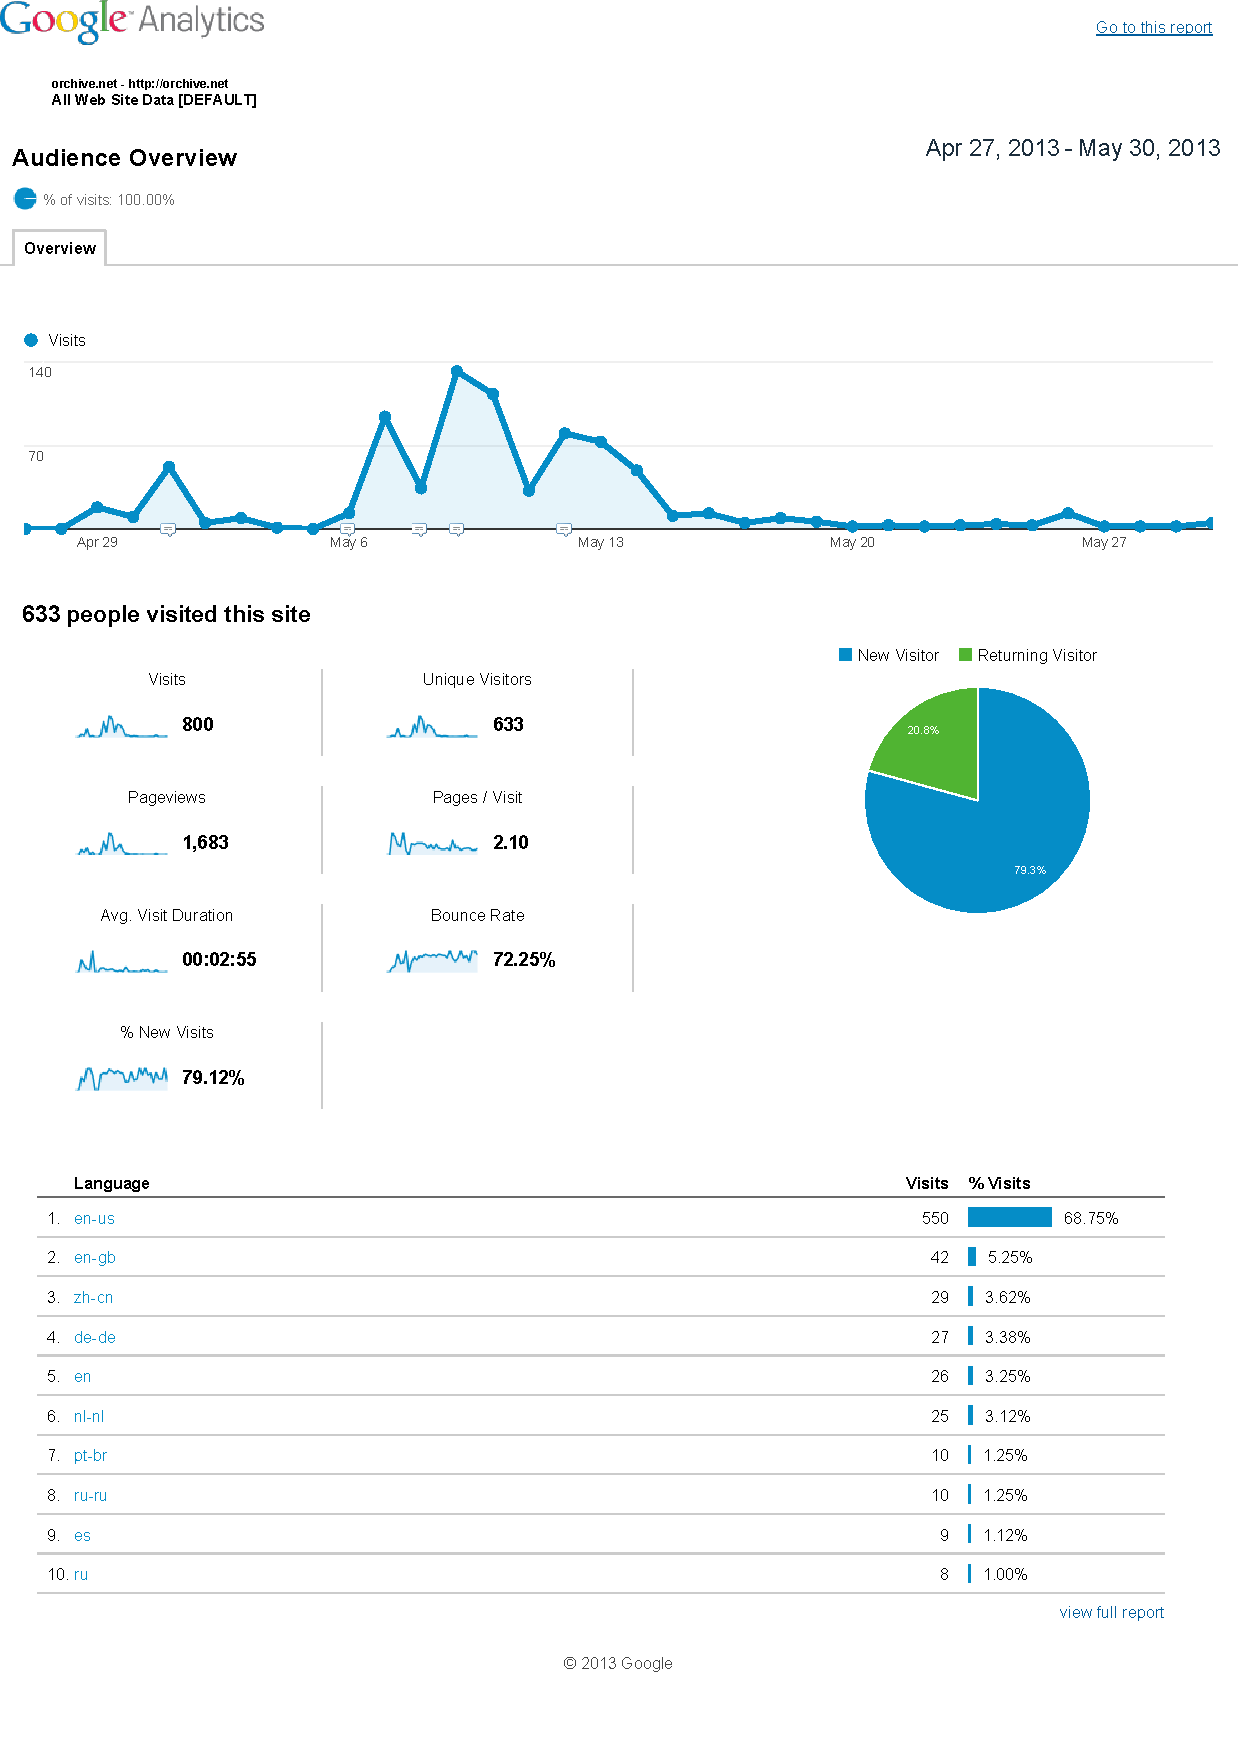
\includegraphics[width=\columnwidth]{figures/orcagameGA}
\caption{orcagameGA}
\label{fig:orcagameGA}
\end{figure}

\begin{figure}[h]
\centering
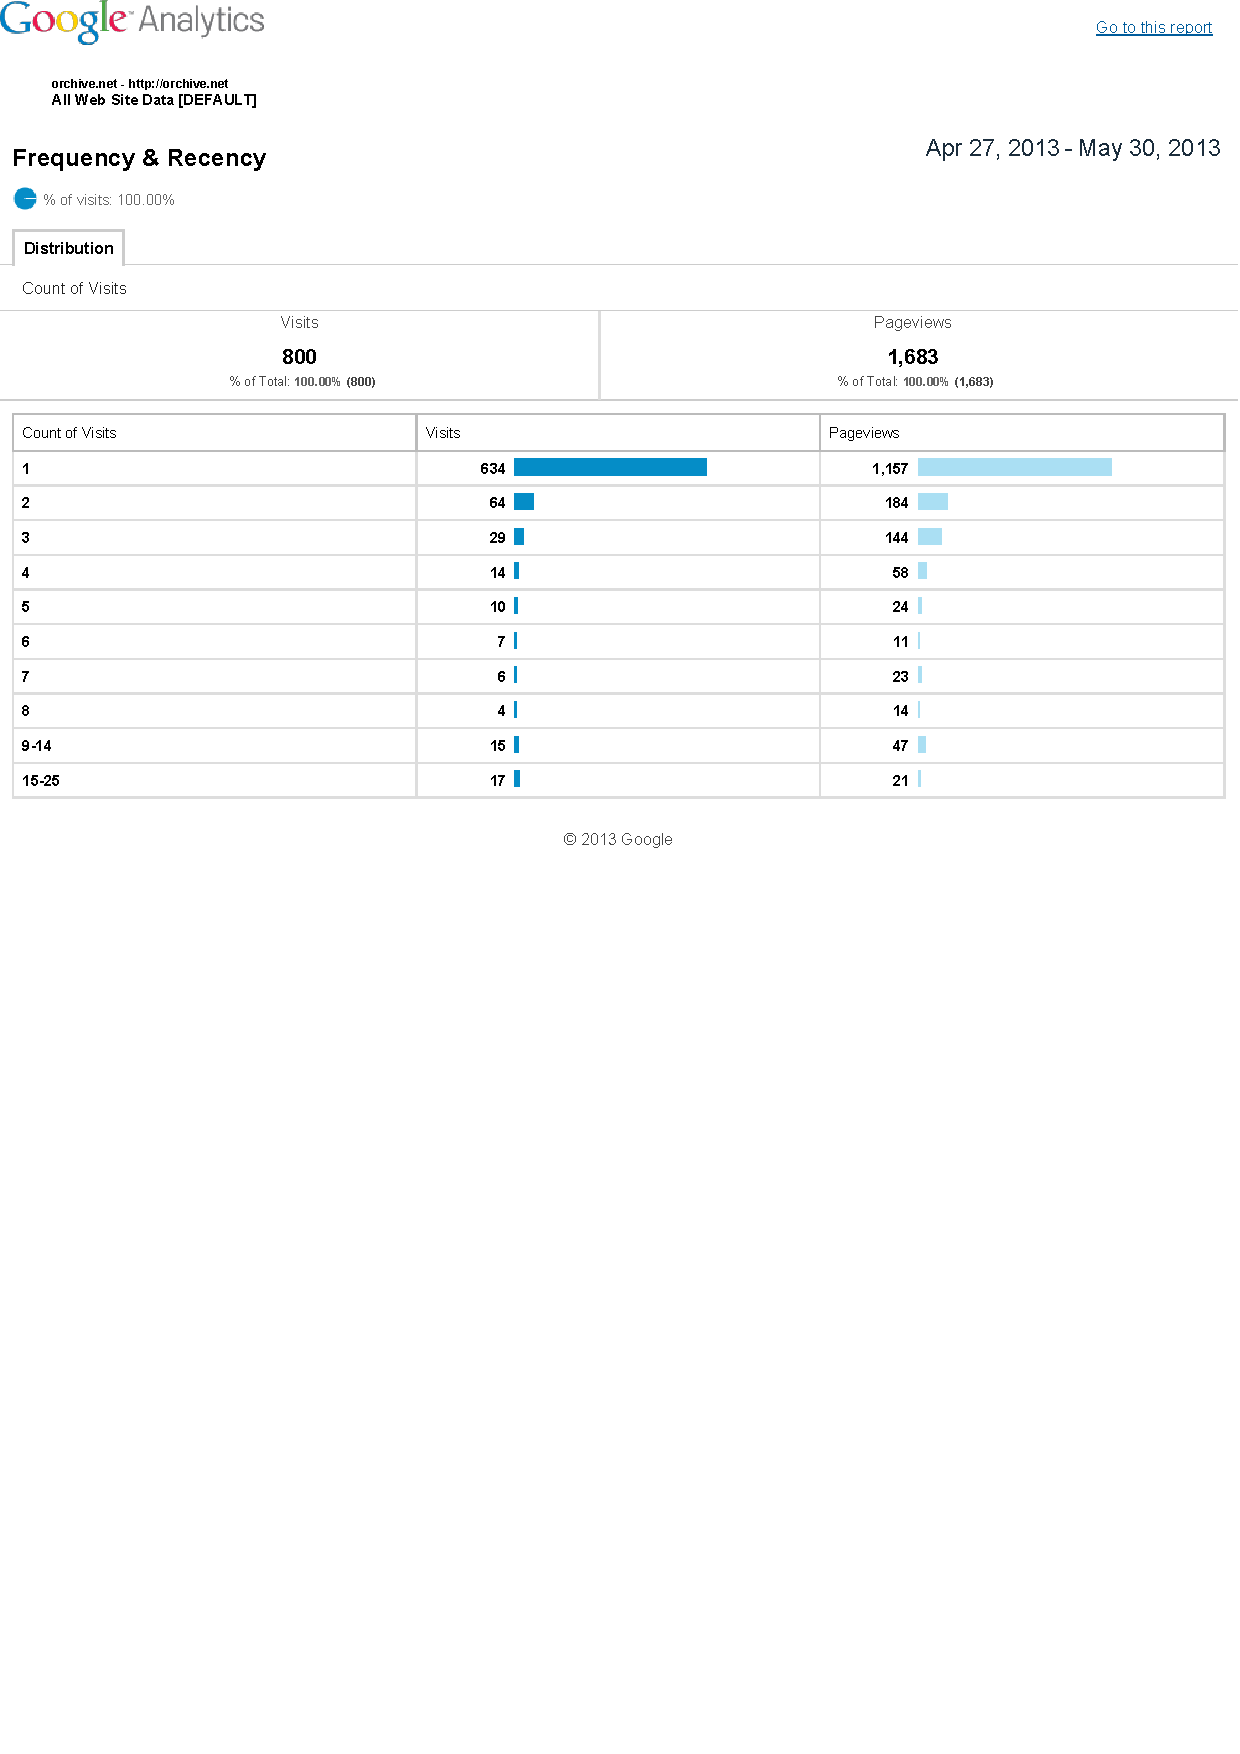
\includegraphics[width=\columnwidth]{figures/orcagameGoogleAnalyticsFrequency}
\caption{orcagameGoogleAnalyticsFrequency}
\label{fig:orcagameGoogleAnalyticsFrequency}
\end{figure}


\begin{figure}[h]
\centering
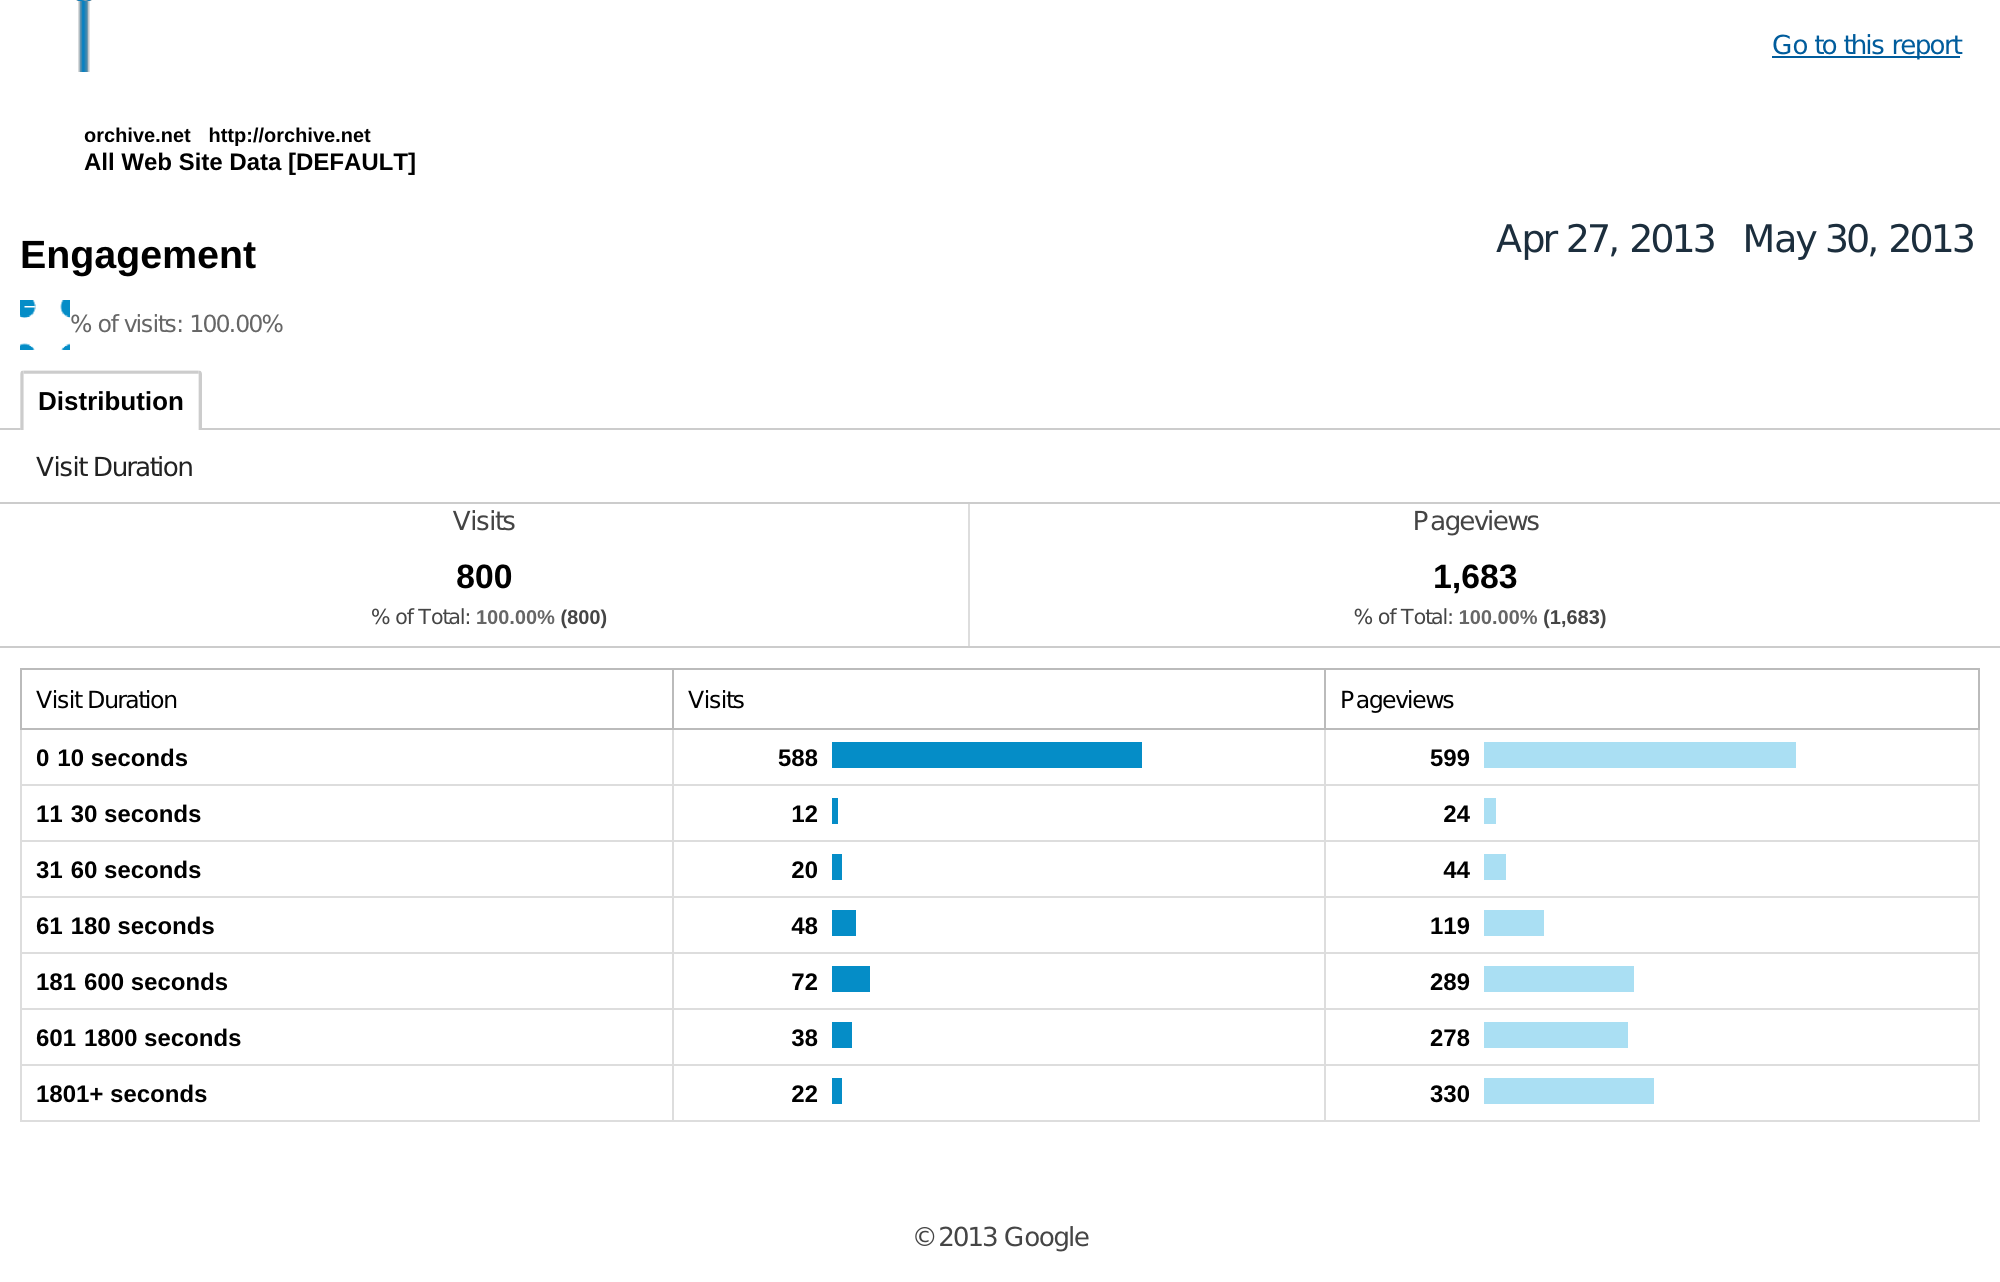
\includegraphics[width=\columnwidth]{figures/orcagameGoogleAnalyticsEngagement}
\caption{orcagameGoogleAnalyticsEngagement}
\label{fig:orcagameGoogleAnalyticsEngagement}
\end{figure}


There were a total of 122 levels created for the game using a custom
Javascript interface, shown in Figure \ref{fig:orcagameGameBuilder}
which had functionality to allow the game designer to search for clips
by call type, call matriline and recording.  This interface was
designed to allow researchers to create their own game levels for the
purpose of training participants.  The earlier static game interface
that was originally built required a programmer to create levels using
JSON, and from interactions with the researchers at OrcaLab, it was
clear that an important feature would be to allow the researchers to
create their own levels.  This interface can also be used with
clips automatically generated by a machine learning classifier to
allow machine generated clips to be annotated by human experts.

The 122 levels in the game were designed to have a wide range of
difficulty, some of the levels asked participants to distinguish
between orcas and other marine mammals such as California Sea Lions
\textit{Zalophus californianus}, Pacific Whitesided Dolphins
\textit{Lagenorhynchus obliquidens} and Humpback Whales
\textit{Megaptera novaeangliae}.  These types of levels were
classified with very high accuracy, with the vast majority being
classified at 100\% accuracy.  

Others asked the users to distinguish between different call types,
for example level 1 which asked the user to distinguish between N01
and N03, N02 and N11, which gave a total classification accuracy
across all users of 88\%, but which the expert users classified with
100\% accuracy.

The most difficult levels asked participants to classify the same call
vocalized by different matrilines, an example of this was a level that
asked the participants to distinguish the N04 call of the A11
matriline from the N04 call of the A12 and A34 matrilines, a task on
which the experts correctly identified 100\% of the time but which all
users classified correctly 72\% of the time.

Suprisingly, ome of the most difficult levels asked participants to
classify orcas based on their pod, a task that experts typically found
easy, but that untrained listeners found very difficult.  One of these
such levels asked participants to classify calls from the Southern
Resident J pod against calls from the G pod and H pod, a task on which
experts got 100\% of the responses correct while untrained listeners
got only 29\% of the responses correct.

A sorted histogram of the percent of correct responses for all 122
game levels is shown in Figure \ref{fig:orcagameSortedAllData}.  From
this we can see that about 2/3 of the game levels were classified with
above 50\% correct responses.

The percent of correct responses broken down by data source is shown
in table form in Table \ref{table:percentCorrect} and graphically in
Figure \ref{figure:percentCorrect}.  From this we can see that
predictably, expert users were able to classify orca calls with the
highest accuracy, with a combined average of 86.4\% classified
correctly.  Participants recruited from Facebook had the second
highest accuracy with 77.3\%.  Surprisingly, participants recruited
from the Orca Live website had a lower average accuracy than those
recruited from Facebook, with an average classification accuracy of
76.3\%.  These participants typically have great experience listening
to orcas, and it would be expected that this familiarity with orca
vocalizations would have given them a considerable advantage in
classifying orca calls.  One possible factor could be that
participants coming from Facebook were also familiar with orca
vocalizations, and that the process of recruitment on Facebook
selected these people with higher probability than people not familiar
with orca vocalizations.

The next highest average came from students recruited from the
Computer Science, with an average accuracy of 60.8\%.  Users from
Google+ had only a 25.8\% accuracy, and those recruited from Google
Ads and Twitter only had a 5\% and 3\% accuracy.  These results are
surprising, and could be due to issues with the instructions, as it
was noted that several of the Google Ads users came from countries
where English was not the native language, including China, Pakistan
and Egypt.  Clearly work on making the application internationalized
is important when targeting these groups of partipants.

\begin{table}
\begin{tabular}{|c|c|}
\hline
User group & Percent Correct \\
\hline
All              &	79.25  \\
Expert           &	86.45  \\
Students         &	60.75  \\
Facebook         &	77.29  \\
Twitter          &	3.07   \\
Google+          &	25.84  \\
OrcaLive         &	76.25  \\
Google Adwords   &	5.45   \\
\hline
\end{tabular}
\caption{}
\label{table:percentCorrect}
\end{table}


Of the total of 3868 classifications of orca vocalizations, different
amounts were classified by different groups of users.  These results
are shown in Table \ref{table:orcagameTotalNum} and graphically in
Figure \ref{fig:orcagameTotalNum}.  The largest number of
classifications came from participants recruited from Facebook, with
855 classifications and the second most came from the Orca Live
website, with 809 participants.  These numbers were not surprising, as
these two groups of participants contained people that were already
interested in orca vocalizations.  One surprising finding was that
although only 9 experts were contacted, they contributed 678
classifications to the database.  There were 337 classifications from
students and professors from the computer science mailing list, 190
from Google Ad words, 134 from Google+, and 10 from Twitter.

\begin{table}
\begin{tabular}{|c|c|}
\hline
User Group      &   \# Classifications \\
\hline
All             &	3868               \\
Expert          &   678                \\
Students        &   337                \\
Facebook        &   855                \\
Twitter         &   10                 \\
Google+         &   134                \\
OrcaLive        &   809                \\
Google Adwords  &   190                \\
other           &   855                \\
\hline
\end{tabular}
\caption{}
\label{table:orcagameTotalNum}
\end{table}


One of the most striking graphs is the number of classifications per
user. This is shown in Figure
\ref{fig:orcagameClassificationsPerUser}, and shows a sorted histogram
of the number of classifications on the vertical axis and the
participant ID on the horizontal axis.  This graph can be interpreted
as that there are few users who are highly engaged with the website
and provide most of the classifications, and that most users only
provide a small number of classifications.  This behaviour has been
seen in other crowdsourcing efforts, and highlights the importance of
building interfaces that are tailored to these types of participants.
	

\begin{figure}[h]
\centering
\includegraphics[width=\columnwidth]{figures/orcagameGameBuilder}
\caption{orcagameGameBuilder}
\label{fig:orcagameGameBuilder}
\end{figure}


\begin{figure}[h]
\centering
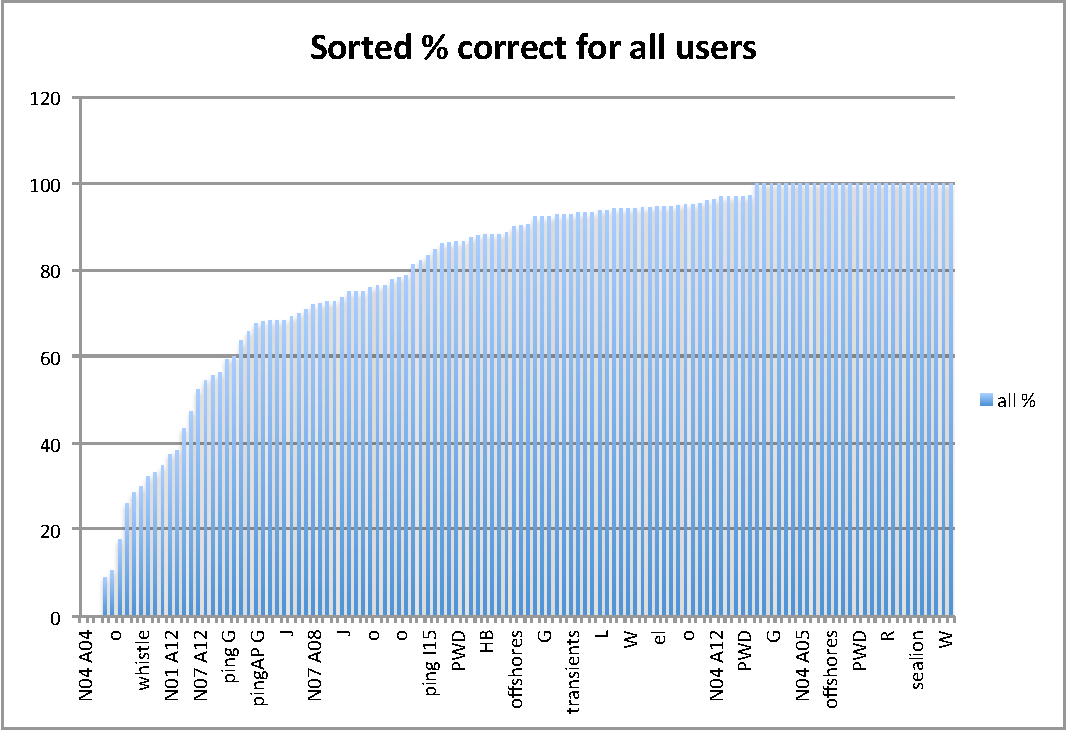
\includegraphics[width=\columnwidth]{figures/orcagameSortedAllData}
\caption{orcagameSortedAllData}
\label{fig:orcagameSortedAllData}
\end{figure}

\begin{figure}[h]
\centering
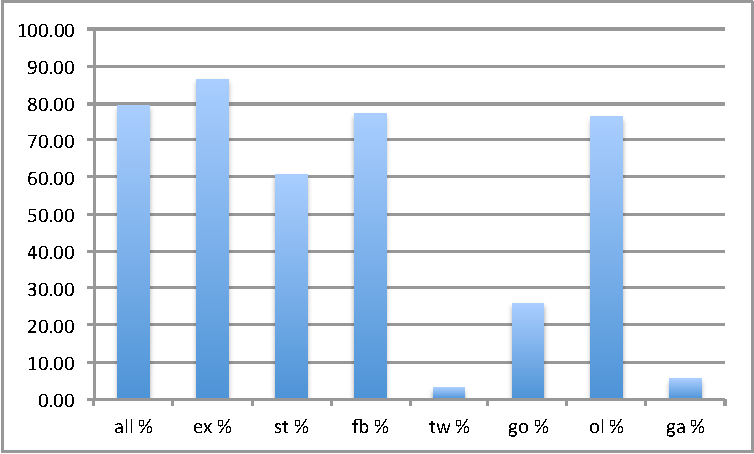
\includegraphics[width=\columnwidth]{figures/orcagamePercentCorrect}
\caption{orcagamePercentCorrect}
\label{fig:orcagamePercentCorrect}
\end{figure}

\begin{figure}[h]
\centering
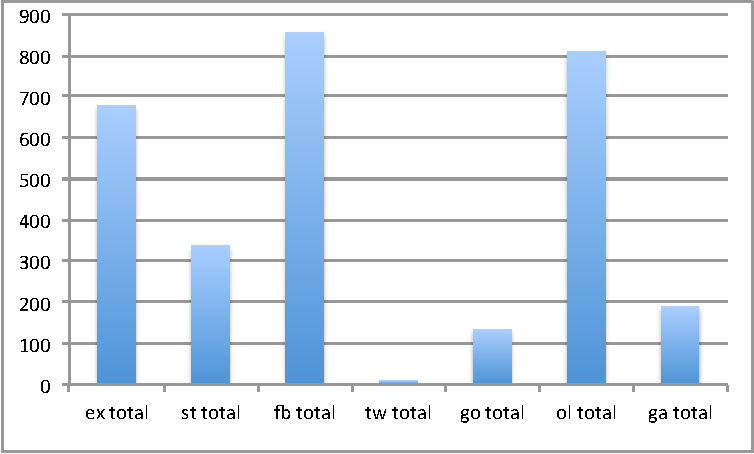
\includegraphics[width=\columnwidth]{figures/orcagameTotalNum}
\caption{orcagameTotalNum}
\label{fig:orcagameTotalNum}
\end{figure}

\begin{figure}[h]
\centering
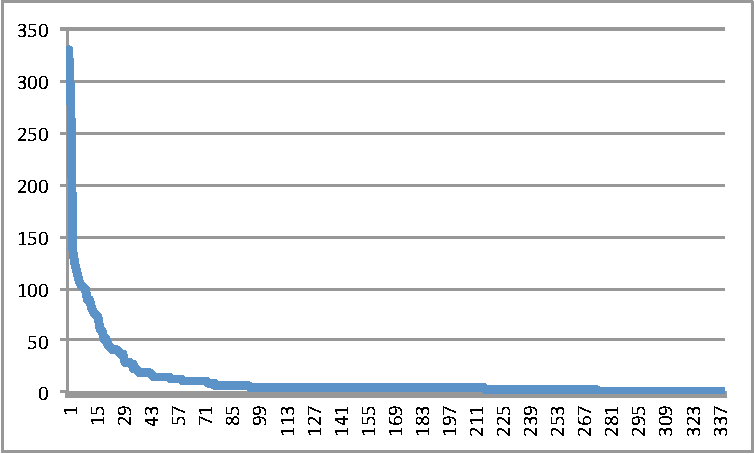
\includegraphics[width=\columnwidth]{figures/orcagameClassificationsPerUser}
\caption{orcagameClassificationsPerUser}
\label{fig:orcagameClassificationsPerUser}
\end{figure}


%% \begin{bchart}[max=50]
%% \bcbar{45}
%% \bcbar{26}
%% \bcbar{31}
%% \label{bchart:test1}
%% \end{bchart}

\begin{figure}[h]
\centering
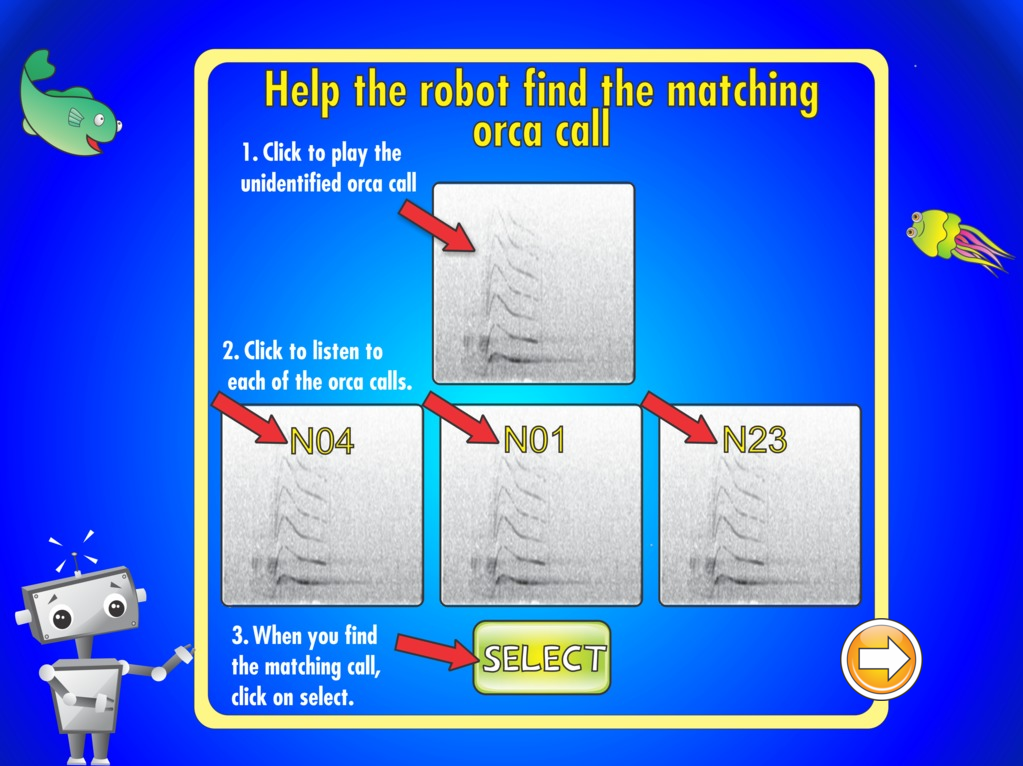
\includegraphics[width=\columnwidth]{figures/orcagameInstructions}
\caption{orcagameInstructions}
\label{fig:orcagameInstructions}
\end{figure}


\begin{figure}[h]
\centering
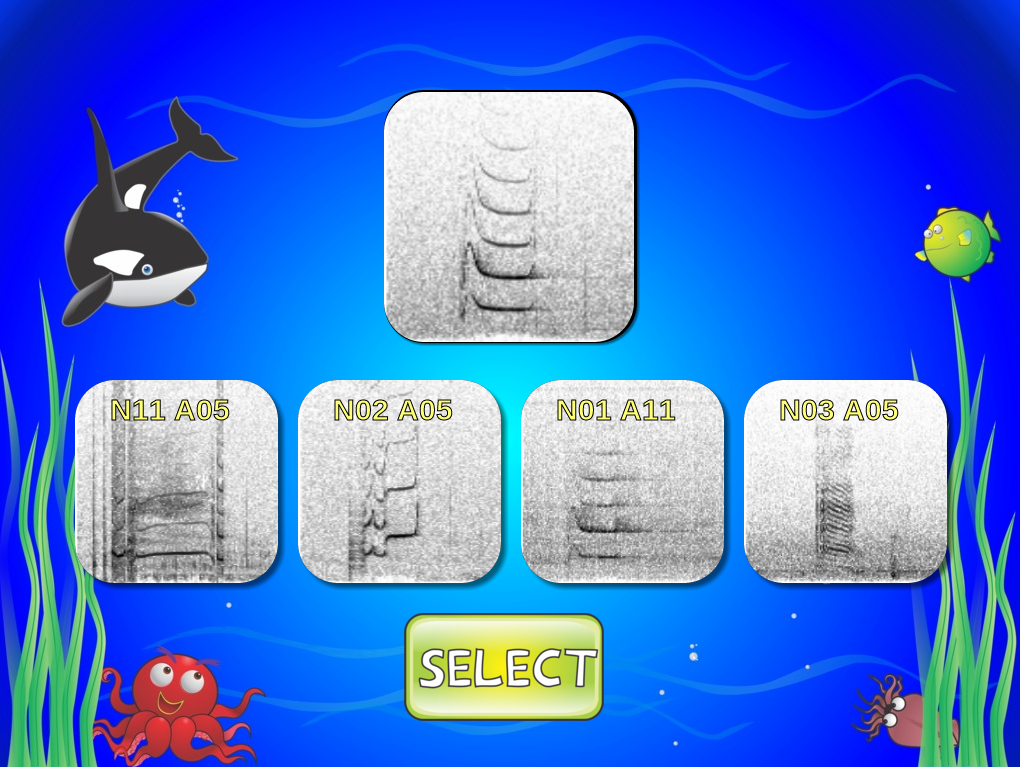
\includegraphics[width=\columnwidth]{figures/orcagame}
\caption{orcagame}
\label{fig:orcagame}
\end{figure}



%% \section{Audio Feature Extraction and Machine Learning}

%% We performed an experiment in which we examined a quantitative ranking
%% task over a diverse set of audio files using tags associated with the
%% audio files.

%% In order to estimate the performance of the learned ranker, we used a
%% standard three-fold cross-validation experimental setup.  In this
%% scheme, two thirds of the data is used for training and one third is
%% used for testing; this process is then repeated for all three splits
%% of the data and results of the three are averaged.  We removed any
%% queries that had fewer than 5 documents in either the training set or
%% the test set, and if the corresponding documents had no other tags,
%% these documents were removed as well.

%% We evaluated our learned model by looking at the precision within the
%% top k audio files from the test set as ranked by each query.
%% Precision at top k is a commonly used measure in retrieval tasks such
%% as these and measures the fraction of positive results within the top
%% k results from a query.

%% The stabilized auditory image generation process has a number of
%% parameters which can be adjusted including the parameters of the PZFC
%% filter and the size of rectangles that the SAI is cut into for
%% subsequent vector quantization.  We created a default set of
%% parameters and then varied these parameters in our experiments.  The
%% default SAI box-cutting was performed with 16 lags and 32 channels,
%% which gave a total of 49 rectangles.  These rectangles were then
%% reduced to their marginal values which gives a 48 dimension vector,
%% and a codebook of size 256 was used for each box, giving a total of 49
%% x 256 = 12544 feature dimensions.  Starting from these, we then made
%% systematic variations to a number of different parameters and measured
%% their effect on precision of retrieval.  For the box-cutting step, we
%% adjusted various parameters including the smallest sized rectangle,
%% and the maximum number of rectangles used for segmentation.  We also
%% varied the codebook sizes that we used in the sparse coding step.

%% In order to evaluate our method, we compared it with results obtained
%% using a very common feature extraction method for audio analysis,
%% MFCCs (mel-frequency cepstral coefficients).  In order to compare this
%% type of feature extraction with our own, we turned these MFCC
%% coefficients into a sparse code.  These MFCC coefficients were
%% calculated with a Hamming window with initial parameters based on a
%% setting optimized for speech.  We then changed various parameters of
%% the MFCC algorithm, including the number of cepstral coefficients (13
%% for speech), the length of each frame (25ms for speech), and the
%% number of codebooks that were used to sparsify the dense MFCC features
%% for each frame.  We obtained the best performance with 40 cepstral
%% coefficients, a window size of 40ms and codebooks of size 5000.

%% We first preprocessed a collection of 1000 music files from 10 genres
%% using a PZFC filterbank followed by strobed temporal integration to
%% yield a set of SAI frames for each file .  We then take this set of
%% SAI and apply the box-cutting technique described above. The followed
%% by the calculation of row and column marginals.  These vectors are
%% then used to train dictionaries of 200 entries, representing abstract
%% ``auditory words'', for each box position, using a k-means algorithm.

%% This process requires the processing of large amounts of data, just to
%% train the VQ codebooks on a training corpus.

%% The resulting dictionaries for all boxes are then used in the MIREX
%% experiment to convert the dense features from the box cutting step on
%% the test corpus songs into a set of sparse features where each box was
%% represented by a vector of 200 elements with only one element being
%% non-zero.  The sparse vectors for each box were then concatenated, and
%% these long spare vectors are histogrammed over the entire audio file
%% to produce a sparse feature vector for each song or sound effect.
%% This operation of constructing a sparse bag of auditory words was done
%% for both the training and testing corpora.

%% \subsection{Audio Feature Extraction}

%% Our evaluation section consists of three parts, in the first we
%% optimize basic audio feature extraction parameters, in the second we
%% use different distributed Machine Learning systems to generate
%% classification results, and in the third we give a report on our
%% experiences with these different platforms for feature extraction and
%% Machine Learning.

%% Our first challenge when dealing with the Orchive is the huge size of
%% the data.  The raw uncompressed .wav files that were digitized from
%% tape take approximately 12TB on disk at the time of this analysis,
%% with more files being added all the time.  In order to determine if we
%% could use a compressed format for doing the audio feature extraction,
%% we compared the results of using a SVM machine to classify the frames
%% of audio.  For the original .wav file we got a classification accuracy
%% of 94.5\%, while a highly compressed 32kbs MP3 gave 93.6\% accuracy.
%% The disk quota on the Westgrid system is set by default at 1TB, so by
%% sacrificing a small amount of accuracy, it was possible to reduce the
%% disk space used from 12TB to 199GB, a 60x savings in space.

%% In order to test the different distributed audio classification
%% systems we first generated a set of training and testing data.  In a
%% previous paper \cite{ness2008}, we were able to obtain a
%% classification performance of 82\% when using a SVM classifier on hand
%% labelled data.  While this performance was adequate when used on a
%% small recording, when run on the entire Orchive, this performance
%% would lead to way too many false positives.  For this paper, we looked
%% in more detail at the training data, and found that while the
%% annotation boundaries were close to the start and end of the
%% vocalization, there was a small amount of silence before and after the
%% vocalization.  Using Audacity, we trimmed out all the silences of a 10
%% second region of audio of orca vocalizations, and did the same to a 10
%% second region of voice notes.  For the background data, we took one
%% hundred 0.1 second regions from random background annotations and
%% joined them together with the Linux audio utility program sox.  The
%% results for this can be found in the first line of table
%% \ref{table:handTrimmed} and had over 99.73\% of the instances
%% classified correctly.  This large jump in performance was unexpected
%% but easily understood, because if feature vectors of silence are
%% labelled as orca, this will cause issues for the classifier.  We then
%% took a 4 minute region of orca calls and voice notes and removed all
%% the silences from both of them.  We then did a preliminary test where
%% we reduced computation time by downsampling the feature vectors at a
%% rate of 100:1, this is shown in the next line of Table
%% \ref{table:handTrimmed}, and followed this by another test at 10:1
%% downsampling and one with no downsampling.  These tests gave
%% classification performance of 95.7\% to 97.7\%.  We then repeated the
%% analysis in our previous paper by using non-hand-trimmed audio, the
%% results are shown in the third section of the table.  We found results
%% from 88.1\% to 93.0\% for 100:1 and no downsampling.  The difference
%% of this result from the previous paper is likely due to the exact
%% training and testing sets used in the two papers.  In the current
%% paper, we are classifying only nearby and isolated orca vocalizations
%% and not the distant or noisy vocalizations, which was a small tweak to
%% the experimental setup that has also helped us to not only achieve
%% better classification performance but to deliver a science goal more
%% pertinent to the bioacoustics researchers who could use the Orchive.

%% \begin{table}
%% \begin{tabular}{|l|c|l|l|r|r|}
%% \hline
%%  trim & time (min)  & ds & features & \# & \% corr.  \\
%% \hline
%%  x & 10 sec  &  1   & all   &    2586  &    99.73  \\
%% \hline
%%  x & 4       & 100  & all   &     606  &    95.71  \\
%%  x & 4       & 10   & all   &    6060  &    97.19  \\ 
%%  x & 4       & 1    & all   &   60596  &    97.72  \\
%%  x & 4       & 100  & mfcc  &     606  &    94.88  \\
%%  x & 4       & 10   & mfcc  &    6060  &    96.03  \\
%%  x & 4       & 100  & yin   &     606  &    xx.xxxx  \\
%%  x & 4       & 10   & yin   &    6060  &    xx.xxxx  \\
%% \hline
%%    & 4       & 100  & all   &     621  &    88.08  \\
%%    & 4       & 10   & all   &    6202  &    92.26  \\
%%    & 4       & 1    & all   &   62023  &    93.01  \\
%%    & 4       & 100  & mfcc  &     621  &    87.76  \\
%%    & 4       & 10   & mfcc  &    6202  &    91.52  \\
%% \hline
%% \end{tabular}
%% \caption{Classification results with hand trimmed orca vocalizations
%%   using bextract to generate audio features and the SVM classifier in
%%   Weka to do a 10-fold crossvalidation of these features.}
%% \label{table:handTrimmed}
%% \end{table}

%% The next task that we worked on was to determine the optimal settings
%% for the audio extraction algorithm.  While there are a number of other
%% audio extraction frameworks in existence like jMIR \cite{mckayphd},
%% SmIrK \cite{wang07} and AIMC \cite{waltersphd}, the Marsyas framework
%% implements most, if not all, of the most popular audio feature
%% extraction algorithms, and presents them as output from the
%% ``bextract'' program as .arff files, which are the input to the Weka
%% suite of Machine Learning programs.  For all experiments here, we use
%% the audio features calculated by Marsyas, however in the future it
%% would be desirable to integrate other audio processing frameworks
%% within OpenMIR.

%% The features output by bextract include the number of zero crossings
%% per unit time, three spectral descriptors (centroid, rolloff, flux),
%% Mel-Frequency Cepstral Coefficients (MFCC) and chroma information
%% based on the western equally tempered scale.  The mean and standard
%% deviation of each of these over a window is then calculated and forms
%% the output.  The first experiment we did was to determine if the MFCC
%% coefficients contained enough information to do the classification on
%% their own, the results for this are shown in Table
%% \ref{table:handTrimmed} in the columns with ``mfcc'' in the
%% ``features'' column.  For the hand trimmed example at a downsampling
%% of 10:1, the performance goes from 97.2\% to 96.0\% which is a small
%% but meaningful difference, especially when one considers how many more
%% false positives one would get when looking at the entire Orchive.  We
%% also tried adding the Yin pitch estimator as another feature in the
%% feature vector output by bextract.  Surprisingly, as one can see in
%% the previous table, the addition of this information actually degraded
%% performance of the classifier.  We are currently investigating how to
%% better incorporate pitch tracking information in our classifiers.

%% The next set of parameters that needed to be optimized were the Window
%% Size and Hop Size of the Digital Signal Processing (DSP) algorithms
%% that take the input audio and calculate spectral information from
%% them, the fundamental basis for which is the Fast Fourier Transform
%% (FFT) algorithm.  One other important input to the bextract feature
%% extraction algorithm is the length of time over which to calculate the
%% statistical properties of the features, this is known in bextract as
%% the ``memory'' and corresponds to the number of frames of features
%% that are accumulated.  The results for this are shown in Table
%% \ref{table:dspParams}.  From this we can see that as we go to longer
%% window sizes, the classification performance increases, and as we go
%% to longer accumulation window sizes, the performance also increases.

%% For our experiments we decided that a good sweet spot was a hop size
%% size of 1024 and a memory of 40 frames, which gave a classification
%% performance of 99.7\%.  80 frames of audio at a sampling rate of 44100
%% samples/sec and a hop size of 1024 would result in a feature length of
%% 1.86 seconds, while 40 frames would only give 0.93 seconds of audio
%% per feature.  Given that orca vocalizations are usually between 0.5
%% and 3 seconds long, we chose a window size of 2048, a hop size of 1024
%% with an accumulator memory of 40 frames.  We did extensive experiments
%% with other values of hopsize, window size and memory that were
%% consistent with these results that are too long to report here.

%% \begin{table}
%% \begin{tabular}{|r|r|r|r|r|r|}
%% \hline
%%  winsize  &  hopsize  &  memory  &  total &   correct  \\
%% \hline
%%      256  &      128  &      20  &        13767   &    97.11  \\
%%      512  &      256  &      20  &        11647   &    96.11  \\
%%     1024  &      512  &      20  &         5923   &    97.74  \\
%%     2048  &     1024  &      20  &         2995   &    98.84  \\
%% \hline
%%      256  &      128  &      40  &        23311   &    96.18  \\
%%      512  &      256  &      40  &        11829   &    97.61  \\
%%     1024  &      512  &      40  &         5991   &    98.86  \\
%%     2048  &     1024  &      40  &         3022   &    99.74  \\
%% \hline
%%      256  &      128  &      80  &        23628   &    97.48  \\
%%      512  &      256  &      80  &        11963   &    98.71  \\
%%     1024  &      512  &      80  &         6044   &    99.74  \\
%%     2048  &     1024  &      80  &         3027   &    99.90  \\
%% \hline
%% \end{tabular}
%% \caption{DSP parameters}
%% \label{table:dspParams}
%% \end{table}

%% \subsection{Machine Learning}

%% The main distributed Machine Learning framework we used was Mahout,
%% which as we previous described is a Java framework for Machine
%% Learning that operates on top of Hadoop.  We investigated a number of
%% its algorithms and found that the Logistic Regression algorithm was
%% the only classification algorithm that was both suitable for our
%% problem and incorporated into the main source code trunk of the code.
%% Our first experiment was just to test the two parameters suggested for
%% tuning this algorithm are shown in Table
%% \ref{table:logisticRegressionTests}, and from these brief experiments
%% it appears the default parameters work best on this data.

%% \begin{table}
%% \begin{tabular}{|r|r|l|}
%% \hline
%%  Passes  & Rate  & Percent Correct                                         \\
%% \hline
%%     100  &    50  &  85.5  \\
%%    1000  &    50  &  85.5  \\
%%     100  &     5  &  83.0  \\
%%     100  &   500  &  85.5  \\
%% \hline
%% \end{tabular}
%% \caption{Logistic regression tests with different parameters.}
%% \label{table:logisticRegressionTests}
%% \end{table}

%% We then took a randomly selected 13GB portion of the 500GB of total
%% (one of the original 37 shards from feature extraction) audio features
%% calculated in the previous section and ran a comparison of the Mahout
%% Logistic Regression algorithm against a simple parallel
%% implementation using a script that runs Weka jobs on multiple
%% computers using the Torque/PBS system on the Westgrid cluster.

%% For this we had our choice of a number of systems on which to run a
%% Mahout/Hadoop cluster on and investigated all of them.  The first was
%% Emulab, which is a fine platform and is very useful for a number of
%% use cases, but for this case of obtaining 10-20 computers and storing
%% substantial amounts of long lived data on them did not fit the Emulab
%% model of running distributed programs on different types of emulated
%% networks on short lived borrowed computers.  While it would have been
%% possible to use Emulab, we were hoping for a longer term solution.
%% Planetlab allows for longer leases, but the large memory and CPU
%% requirements of our program made this less feasible as well.  We
%% attempted to obtain machines on the GeniCloud at HP, but were unable
%% to obtain the machines in the end.  The best solution we felt was to
%% use the six GreenGeni nodes at UVIC and setup a Hadoop cluster on
%% these.  We attempted to do this for quite some time, but ran into a
%% number of odd port issues.  We suspect the problem are concurrently
%% running Swift and Disco installs on these machines that might be
%% utilizing these ephemerally used ports.  The problem could also be due
%% to a misconfiguration of the networking hardware.  Another solution
%% would be to use the Amazon EC2 cluster service, or even their Elastic
%% MapReduce service, a service that is easy to setup and use, however,
%% costs for it can add up quickly.  For the results in this paper we use
%% a mini 2-node Hadoop cluster that was setup in our lab in a controlled
%% setting, this was simple to install and get results from.  In the near
%% future we hope to setup a larger Hadoop cluster and to rerun these
%% jobs with more processors.

%% For all of our analysis here, we took one of the 37 splits of the
%% original data analyzed by bextract.  This file was 13GB in size and
%% contained 22486467 lines.  For the following experiments we took the
%% first $n$ lines of this file where $n$ started at 10 and increased to
%% 10,000,000 in powers of 10.

%% For the first experimental condition, the Logistic Regression
%% Classifier as implemented in Mahout was used, and Hadoop was used as
%% the underlying system below Mahout.  The Logistic Regression
%% classifier as implemented by default in Mahout can only take two
%% classes as input, so for all these experiments we used only orca and
%% background as the training data.  The timing results of Logistic
%% Regression in Mahout are shown in Table
%% \ref{table:machineLearningTiming1}.  As we can see, the system is very
%% fast, even classifying a million instances only takes one minute on a
%% small two node cluster.  As the number of instances increases, the
%% time increases quickly, it would be interesting to see this with a
%% larger cluster of 10 or more nodes.

%% For the second experimental condition, we used the Weka Machine
%% Learning package and ran it with it's Logistic Regression engine.
%% This was run on the Hermes cluster at Westgrid, and for these tests,
%% only 10 nodes were run at one time, although scaling up is as simple
%% as splitting the input file into more chunks and starting more jobs.
%% Weka is a Java program, and thus incurs a certain startup time when
%% creating and setting up the JVM and other resources.  This is
%% reflected in the results in Table \ref{table:machineLearningTiming2}
%% where up to 100000 instances the run times are all around 6 seconds.
%% The third experimental condition was to use Weka again, but this time
%% with its SVM engine.  Interestingly, the time that the SVM took to run
%% was about the same as the Logistic Regression, even though SVM is
%% typically be a considerably better classifier than Logistic
%% Regression.

%% In the final experiment, PSVM was run on the Checkers cluster at
%% Westgrid.  It was unable to be run on the Hermes and Nestor clusters
%% due to the use of MPICH2 by PSVM and the use of the original MPI
%% version 1.0 on the clusters.  This program takes advantage of the MPI
%% message passing library to communicate between a number of different
%% computers, and for the experiments shown below, we used 4 processors.
%% It should be noted that at least on the Checkers cluster, it is
%% difficult to reserve a block of 5 computers at once, much more
%% difficult than starting 5 individual jobs.  Depending on the cluster
%% you have access to, this may or may not be a problem.


%% \begin{table}
%% \begin{tabular}{|l|r|r|r|}
%% \hline
%%  system  &  \# proc.  &  num instances  &  time (sec)  \\
%% \hline
%%  Mahout  &     2          &            100  &       0.55  \\
%%  Mahout  &     2          &           1000  &       0.89  \\
%%  Mahout  &     2          &          10000  &       1.45  \\
%%  Mahout  &     2          &         100000  &       6.69  \\
%%  Mahout  &     2          &        1000000  &      57.90  \\
%%  Mahout  &     2          &       10000000  &     566.35  \\
%%  Mahout  &     2          &       22486467  &     566.35  \\
%% \hline
%%  PSVM     &           10  &            100  &     2  \\
%%  PSVM     &           10  &           1000  &     1  \\
%%  PSVM     &           10  &          10000  &     1  \\
%%  PSVM     &           10  &         100000  &     50  \\
%%  PSVM     &           10  &        1000000  &     635  \\
%%  PSVM     &           10  &       10000000  &       \\
%%  PSVM     &           10  &       22486467  &       \\
%% \hline
%% \end{tabular}
%% \caption{Timing results for all Machine Learning Algorithms}
%% \label{table:machineLearningTiming1}
%% \end{table}

%% \begin{table}
%% \begin{tabular}{|l|r|r|r|}
%% \hline
%%  system  &  \# proc.  &  num instances  &  time (sec)  \\
%% \hline
%%  Weka : LogReg    &           10  &            100  &        6.03  \\
%%  Weka : LogReg    &           10  &           1000  &        6.05  \\
%%  Weka : LogReg    &           10  &          10000  &        6.09  \\
%%  Weka : LogReg    &           10  &         100000  &        7.55  \\
%%  Weka : LogReg    &           10  &        1000000  &       31.24  \\
%%  Weka : LogReg    &           10  &       10000000  &      183.74  \\
%%  Weka : LogReg    &           10  &       22486467  &      233.99  \\
%% \hline
%%  Weka : SVM     &           10  &            100  &        5.38  \\
%%  Weka : SVM     &           10  &           1000  &        5.35  \\
%%  Weka : SVM     &           10  &          10000  &        5.15  \\
%%  Weka : SVM     &           10  &         100000  &        7.53  \\
%%  Weka : SVM     &           10  &        1000000  &       28.66  \\
%%  Weka : SVM     &           10  &       10000000  &      182.61  \\
%%  Weka : SVM     &           10  &       22486467  &      	  \\
%% \hline
%% \end{tabular}
%% \caption{Timing results for all Machine Learning Algorithms}
%% \label{table:machineLearningTiming2}
%% \end{table}


%% \section{Orca}

%% \begin{table}
%% \caption{Classification Performance}
%% \begin{tabular}{|c|c|c|} \hline

%% Dataset&Correctly Classified Instances&Percent Correct\\ \hline

%% 446A & 30403 & 90.31\\ \hline
%% 446B & 33701 & 81.97\\ \hline
%% 447B & 23013 & 73.65\\ \hline
%% 448A & 15307 & 58.04\\ \hline
%% 448B & 20822 & 74.61\\ \hline
%% 449B & 25239 & 81.17\\ \hline
%% 450A & 31872 & 87.85\\ \hline
%% 450B & 23916 & 93.51\\ \hline
%% 451A & 54281 & 89.74\\ \hline
%% 451B & 25528 & 69.91\\ \hline
%% \hline\end{tabular}
%% \end{table}


%% \begin{table}
%% \centering
%% \caption{Recording-specific classification performance}
%% \begin{tabular}{|c|c|c|c|c|} \hline

%% &\multicolumn{2}{|c|}{Naive bayes}&\multicolumn{2}{|c|}{SMO}\\
%% &\multicolumn{2}{|c|}{\% correct}&\multicolumn{2}{|c|}{\% correct}\\ \hline
%% &self&train with&self&train with\\
%% &&remaining&&remaining\\ \hline

%% 446A  &  89.42  &  93.10  &  95.00  &  73.39\\ \hline
%% 446B  &  63.45  &  77.66  &  85.85  &  70.23\\ \hline
%% 447B  &  75.46  &  57.32  &  82.02  &  68.17\\ \hline
%% 448A  &  52.18  &  61.02  &  81.57  &  62.24\\ \hline
%% 448B  &  84.63  &  67.62  &  83.64  &  67.87\\ \hline
%% 449B  &  82.24  &  51.85  &  86.41  &  75.72\\ \hline
%% 450A  &  94.66  &  90.91  &  96.12  &  91.58\\ \hline
%% 450B  &  83.65  &  96.27  &  99.29  &  94.92\\ \hline
%% 451A  &  70.92  &  89.58  &  97.04  &  78.72\\ \hline
%% 451B  &  74.18  &  33.73  &  82.34  &  50.88\\ \hline
%% \end{tabular}
%% \label{table:classification}
%% \end{table}


%% In order to explore whether this idea would work for our data, we 
%% created a representative database consisting of 10 excerpts from 
%% our recordings with each excerpt lasting between 5 and 10 minutes. 
%% Table ~\ref{table:classification} shows classification results using 
%% 10-fold cross-validation for each particular recording using a
%% recording specific classifier as well as using a classifier trained 
%% on the entire dataset. Two classifiers are used: a simple Naive Bayes
%% classifier (NBS), as well as a Support Vector Machine (SVM). The results shown 
%% are based on the use of the standard Mel-Frequency Cepstral
%% Coefficients (MFCC) as audio features. The ``self'' column shows the 
%% classification accuracy results of using a recording-specific
%% classifier, whereas the ``remaining'' columns 
%% shows the classification accuracy results using the remaining nine
%% recordings. As can be seen, recording-specific classifier can generate
%% significantly better results than generalized classifiers, which is not 
%% surprising as they adapt to the specific data of the recording. This
%% justifies the use of their annotation results to labeled the unlabeled 
%% parts of the audio recording. 


%% In order to systematically explore the different strategies for Orca
%% call retrieval we utilized a dataset consisting of 185 recordings of
%% vocalizations. They have been annotated using the Orchive
%% collaborative user interface and classified into 4 discrete call types
%% by volunteers. The ground truth labels have been verified by
%% experts. Table ~\ref{table:dataset} shows the composition of the
%% dataset used for evaluation. We use two established evaluation metrics
%% that measure the retrieval effectiveness. Precision at 1 is simply the
%% number of queries for which the first retrieved call has the same
%% class as the query. The mean average precision (MAP) is the most
%% frequently used summary measure of a ranked retrieval run. Average
%% precision of a single query is the mean of the precision scores after
%% each relevant document has been retrieved. The value for the run (a
%% set of queries) is the mean of the individual average precision
%% scores. MAP combines aspects of both precision and recall and rewards
%% returned relevant items higher in the list.


%% \begin{table} 
%% \begin{center}
%% \caption{Dataset composition and MAP scores for best configuration
%%   (Hertz frequency scale, SACF pitch extractor and DTW matching) } 
%% \begin{tabular}{|l|c|c|c|c|}
%% \hline
%% Call Type     & N1      & N3      & N4 & N47 \\ 
%% \hline 
%% Instances     & 36      & 56      & 60  &  33 \\ 
%% \hline 
%% MAP            & 0.63   &  0.94   & 0.78  & 0.58  \\ 
%% %  Precision@1 &      &       &      &       \\ 
%% \hline 
%% \end{tabular} 
%% \label{table:dataset}
%% \end{center}
%% \end{table} 


%% Table ~\ref{table:dataset} shows the best MAP scores achieved for each
%% type of call. As can be seen there is large variance in the MAP score
%% for different types of calls. For example retrieval of N3 calls is
%% very robust but retrieval of the N47 calls is not as much. These
%% differences are also observed in the human classification of these
%% calls. 

%% Table ~\ref{table:dataset_map} shows the MAP scores and
%% average precision score at 1 over the entire dataset for combinations
%% of different representations and pulse rate extraction strategies. As
%% can be seen, the SACF pitch extractor is the best performing pitch
%% extraction method independently of the retrieval strategy. The DTW
%% matching is also the best performing retrieval strategy. It is hard to
%% draw any conclusions with respect to SACF performing better than the
%% other two pitch extractors. The better results obtained using the DTW
%% retrieval strategy indicate there is important non-uniform timing
%% variation in the structure of these calls. 

%% We have also conducted experiments with different frequency scale
%% representations such as the Bark-scale \cite{zwicker1961} and
%% logarithmic frequency but in all configurations they performed worst
%% than the default linear frequency representation in Hertz.

%% \begin{table} 
%% \begin{center}
%% \caption{Mean Average Precision Scores for different pitch extraction 
%% and retrieval strategies} 
%% \begin{tabular}{|l|c|c|c|}
%% \hline   
%%               & Features           & Contour      & DTW   \\
%% \hline 
%% PRAAT         & 0.38               & 0.52         & 0.67  \\
%% \hline 
%% YIN           & 0.50               & 0.51         & 0.72  \\ 
%% \hline 
%% SACF          & 0.63               & 0.66         & 0.77  \\ 
%% \hline 
%% \end{tabular} 
%% \label{table:dataset_map}
%% \end{center}
%% \end{table} 


%% \begin{table} 
%% \begin{center}
%% \caption{Average Precision at 1 scores for different pitch extraction 
%% and retrieval strategies} 
%% \begin{tabular}{|l|c|c|c|}
%% \hline   
%%               & Features & Contour & DTW   \\
%% \hline 
%% PRAAT         &    0.38  & 0.40    &  0.40  \\ 
%% \hline 
%% YIN           &    0.77  & 0.72    &  0.95 \\ 
%% \hline 
%% SACF          &    0.79  &  0.82   &  0.95 \\ 
%% \hline 
%% \end{tabular} 
%% \label{table:dataset_prec1}
%% \end{center}
%% \end{table} 


%% \begin{table}
%% \begin{tabular}{|l|l|l|l|}
%% top-k & SAI & MFCC & percent error reduction \\ \hline
%% 1 & 27 & 33 & 18 \% \\
%% 2 & 39 & 44 & 12 \% \\
%% 5 & 60 & 62 & 4 \% \\
%% 10 & 72 & 74 & 3 \% \\
%% 20 & 81 & 84 & 4 \% \\
%% \end{tabular}
%% \caption{A comparison of the best SAI and MFCC configurations.  This
%%   table shows the percent error at top-k, where error is defined as 1
%%   - precision.}
%% \label{table:topk}
%% \end{table}

%% \begin{table}
%% \centering
%% \begin{tabular}{|l|l|}
%% Algorithm & Classification Accuracy \\\hline
%% SAI/VQ & 0.4987 \\
%% Marsyas MFCC & 0.4430 \\
%% Best & 0.6526 \\
%% Average & 0.455 \\
%% \end{tabular}
%% \caption{Orca call train/test classification task}
%% \label{table:classical}
%% \end{table}

%% \begin{table}
%% \centering
%% \begin{tabular}{|l|l|}
%% Algorithm & Classification Accuracy \\\hline
%% SAI/VQ &  0.4861 \\
%% Marsyas MFCC & 0.5750\\
%% Best &  0.6417 \\
%% Average &  0.49 \\
%% \end{tabular}
%% \caption{Bird song train/test classification task}
%% \label{table:mood}
%% \end{table}

%% There are three main areas that we investigate in this work.  The
%% first is to determine which of the approximately 22,000 recordings in
%% the Orchive contain acceptably low levels of boat noise.  The second
%% is to pull out individual clips of orca vocalizations from these
%% quieter recordings.  The third task is to classify these individual
%% vocalizations into call classes according to classes previously
%% identified by whale researchers.

%% In this work we subdivide our work into three sections, in the first,
%% we classify whole recordings into ``silent'' and ``noisy'', in the
%% second we segment the audio recording into ``background'', ``orca'',
%% and ``voice note''.  In the third we classify small clips of known
%% orca vocalizations into different call types, as identified in a
%% pre-existing orca call catalog.

%% \subsection{Silent and Noisy recordings}

%% To classify whole recordings into the classes silent and noisy, we
%% first collected a set of 100 examples of silent recordings, and a set
%% of 100 examples of noisy recordings.  We then extracted audio features
%% from these recordings and output these as a .arff file.  This file was
%% then processed with the SMO SVM classifier in Weka to generate the
%% classification accuracy numbers shown in the next section.  To
%% classify recordings, we extracted audio features from each clip of an
%% audio file which were output as a .arff file and used a C++ program
%% that used libSVM to classify each 1 second clip of the audio file.

%% \subsection{Orca, Voice Note, Background}

%% To segment recordings into Orca, Voice Note and Background, we used a
%% C++ program that combined an audio feature extraction engine with an
%% SVM classifier. We trained this classifier on different amounts of
%% data and evaluated the performance of each of the resulting Support
%% Vector Machines.  The C++ program classified each frame of audio
%% features into a class, and then performed a neighborhood voting
%% scheme, where a 1 second window of multiple 20ms frames were used, and
%% the class that had the most number of frames that were classified as
%% that class was output.  For example, if 80 frames were classified as
%% orca, 15 as voice and 5 as background, the classifier would output
%% ``orca 80'' for that 1 second section of audio.

%% In order to classify orca calls according to a pre-defined call
%% catalog, 325 clips containing orca vocalizations were classified by
%% hand into six classes of common calls, which were ``N1'', ``N3'',
%% ``N4'', ``N7'', ``N9'' and ``N47''.  A single audio feature vector for
%% each clip was calculated which contained the mean and standard
%% deviation for the audio features mentioned above.  This gave a feature
%% vector of size 68 which was output in .arff format.  These files were
%% then used as input to Weka and three different classifiers were used,
%% including J48, Naive Bayes and the SMO SVM classifier.

%% \section{Results}\label{sec:results}

%% \subsection{Audio Feature Extraction}

%% We did a parameter search over window size, hop size and memory size.
%% The results of this are shown in Table \ref{table:afe}.  From this
%% table we can see that the optimal setting of window size and hop size
%% is 2048 and 1024 and the optimal window size is 40 frames.  While it
%% would be possible to go to large window sizes, in our experience this
%% blurs out the frequency to an unacceptable level in other Machine
%% Hearing tasks and makes segmentation of the audio problematic.

%% \begin{table}
%% \centering
%% \caption{Audio Feature Extraction}
%% \begin{tabular}{ccccc} 
%% \hline
%% Window Size & Hop Size & Memory & \% correct & \# data points \\  \hline
%% \\ 
%% 1024 & 512  & 1  & 83.5 & 282899 \\
%% 1024 & 512  & 10 & 87.7 & 282899 \\
%% 1024 & 512  & 40 & 92.5 & 282899 \\
%% 2048 & 1024 & 1  & 84.1 & 143049 \\
%% 2048 & 1024 & 10 & 91.3 & 143049 \\
%% 2048 & 1024 & 40 & 93.7 & 143049 \\
%% \\ \hline
%% \end{tabular}
%% \label{table:afe}
%% \end{table}


%% \subsection{Silent and Noisy recordings}

%% As training data for this task, we labeled 100 instances of audio as
%% ``silent'' and 100 instances of ``not-silent'' and extracted a variety
%% of audio features from these files, including MFCC coefficients,
%% general spectral descriptors such as the centroid frequency, Rolloff
%% frequency and flux, and the number of zero crossings per window.

%% For this experiment, we extracted a single summary vector for each
%% audio clip containing 68 elements, which were the mean and standard
%% deviation for each of the audio features given above.  We generated
%% audio features for these 200 instances and classified them using the
%% SMO SVM classifier in Weka.  From this we obtained a classification
%% accuracy of 82.5\%.

%% To provide a summary of the recordings in the Orchive, 6 clips of 1
%% second in duration were extracted from each recording.  This gave a
%% total of 125,347 clips, totaling 2089 hours of audio.  We extracted
%% the same features as those extracted from the training data above and
%% output these vectors as a .arff file.  These vectors were then used as
%% training data for an SVM classifier implemented in C++ and using
%% libSVM \cite{cc01} as the classifier. We took each of the 125,347
%% clips of audio and classified each one of them into the classes
%% ``noisy'' and ``silent''.  Of these, 87,657 were classified as noisy
%% and 37,690 were classified as quiet.  The quiet recordings would
%% provide for a good dataset for researchers to examine first, and could
%% then move on to progressively more difficult recordings as their
%% research project required more data.

%% \subsection{Orca, Voice Note, Background}

%% As an initial study, a total number of 3265 samples of data labeled
%% with ``orca'', ``voice'' and ``background'' was used to train a Naive
%% Bayes classifier in Weka with default parameters.  This gave a
%% classification accuracy of 68.3\%.  The same data was also used to
%% train a SVM using the SMO classifier in Weka with default parameters
%% which gave a classification accuracy of 77.6\%.  The confusion matrix
%% is shown below.

%% \begin{verbatim}
%%     a    b    c   <-- classified as
%%   886  298    2 |    a = b
%%   376 1516    3 |    b = o
%%    34   17  133 |    c = v
%% \end{verbatim}

%% It can be seen from this confusion matrix that background and orca
%% vocalizations are labeled as each other quite often.  In the Orchive,
%% the majority of the audio data is of background recordings, and an
%% important task is for the machine learning system to distinguish
%% background recordings from orca vocalizations.  If our classifier
%% gives a large number of false positives, it will be difficult for
%% researchers to use this data to find orca vocalizations.

%% Upon further examination it became clear that the problem was that the
%% large amount of background noise in the recordings was difficult for
%% our chosen audio features.  It was then decided to instead train a
%% classifier to identify clearly identifiable orca vocalizations, and
%% then extract these clear vocalizations from the archive for further
%% processing.  From the results of the previous section, where we
%% identified a large number of recordings with silence in them, this
%% limited amount of data would still represent a large dataset to study.

%% To improve classification accuracy, a set of 725 audible orca recordings
%% was chosen using the orcaGame interface.  534 clear voice recordings
%% were also collected, and 1539 background recordings were collected.
%% We then randomized selected subsets of 10, 50 and 500 recordings from
%% each of these collections and trained a machine learning classifier on
%% each of these collections.  To test these classifers, we used a
%% separate set of recordings, and used a neighbourhood voting method,
%% where each 20ms section of audio was classified by a SVM classifier,
%% and then the results of 1 second of these were collected.  The scheme
%% we used is described in the Data Mining section above.

%% The results from this are shown in Table \ref{table:obv}.  From this
%% we can see that the classification performance for classifying orca,
%% background and voice is approximately 85\%-89\%.  We are currently
%% running this classifier on all recordings in the Orchive, but due to
%% it's slow speed, are looking for ways to downsample this data and
%% provide a performance boost.


%% \begin{table}
%% \centering
%% \caption{Orca / Background / Voice}
%% \begin{tabular}{cccccc} 
%% \hline
%% \# Training & Time & Time to classify & \% correct & \% background & \% voice  \\  
%% samples & to train & classify 1 sec & orca & background & voice \\ \hline
%% \\ 
%% 150   & 525    & 0.1 sec  & 64.1 \%  & 46.7 \%  & 91.7 \% \\
%% 300   & 2103   & 0.5 sec  & 79.6 \%  & 66.0 \%  & 93.5 \% \\
%% 1500  & 29025  &   2 sec  & 84.6 \%  & 85.3 \%  & 88.9 \% \\
%% \\ \hline
%% \end{tabular}
%% \label{table:obv}
%% \end{table}


%% \subsection{Orca call classification}

%% Using the Orchive and orcaGame web interfaces, we created a collection
%% of 319 calls of 6 classes, these included the common calls ``N1'',
%% ``N3'', ``N4'', ``N7'', ``N9'' and ``N47''.  Audio features for each
%% 20ms audio frame of these files were generated, these included the
%% MFCC coefficients, Centroid, Rolloff, Flux and Zero crossings.  The
%% mean and standard deviation for each of these features were then
%% calculated and were output as a .arff file.  

%% These were then classified with Weka using the J48 tree classifier,
%% which gave an accuracy of 58\%.  We next tried the Naive Bayes
%% classifier which gave an accuracy of 64.6\%.  The SMO SVM classifier
%% produced the best results, giving an accuracy of 75.9\%.

%% The confusion matrix for the SVM classifier is shown below.  From this
%% we can see that most of the classes are classified correctly.  One
%% interesting point is that there is some confusion between the N7 and
%% N9 calls, and it can be noted that these calls are often confused with
%% each other by humans as well.

%% \begin{verbatim}
%%  a  b  c  d  e  f   <-- classified as
%%  30  0  0  1  0  4 |  a = N1
%%   1 53  2  0  0  0 |  b = N3
%%   0  1 80  9  1  2 |  c = N4
%%   0  0 32  0  0  1 |  d = N47
%%   0  2  1  0 15 13 |  e = N7
%%   3  0  2  0  2 64 |  f = N9
%% \end{verbatim}


%% In this work we first annotated a large number of clips from the
%% Orchive, and in doing so, doubled the number of annotations in the
%% Orchive that had been generated by 29 scientists over 4 years.  This
%% set of annotations labeled clips as orca, background or voiceover.

%% Because of the amount of boat noise in a large number of these clips,
%% early results with a SVM classifier gave the disappointing result of
%% approximately 77\% accuracy.  We then used the orcaGame citizen
%% science mini-game to refine the classification of these clips into
%% distant orcas and more clear orca calls, and also used this interface
%% to classify clips into the classes noisy and silent.

%% These noisy and silent clips were used to train a machine learning
%% classifier that was then used to classify all the recordings in the
%% orchive into silent and noisy, which gave a total of 37,690 silent
%% clips that would be useful for early work on call classification.

%% We then used the clear orca calls, background calls and voice notes to
%% train a machine learning classifier to segment recordings and pull out
%% clips of isolated orca vocalizations.  With 1500 training clips we
%% were able to get an accuracy of 84.6\% in classifying orca calls and
%% approximately the same accuracy with background and voice clips.

%% Finally, we classified a sample of orca vocalizations by hand into a
%% set of 6 call classes, and using an SVM classifier were able to get a
%% classification accuracy of 75.9\%.

%% In conclusion, this project was quite successful, and also more
%% importantly, has laid the groundwork for an ongoing study in which we
%% are classifying all the audio in the entire Orchive.

%% In order to systematically explore the different strategies for Orca
%% call retrieval we utilized a dataset consisting of 185 recordings of
%% vocalizations. They have been annotated using the Orchive
%% collaborative user interface and classified into 4 discrete call types
%% by volunteers. The ground truth labels have been verified by
%% experts. Table ~\ref{table:dataset} shows the composition of the
%% dataset used for evaluation. We use two established evaluation metrics
%% that measure the retrieval effectiveness. Precision at 1 is simply the
%% number of queries for which the first retrieved call has the same
%% class as the query. The mean average precision (MAP) is the most
%% frequently used summary measure of a ranked retrieval run. Average
%% precision of a single query is the mean of the precision scores after
%% each relevant document has been retrieved. The value for the run (a
%% set of queries) is the mean of the individual average precision
%% scores. MAP combines aspects of both precision and recall and rewards
%% returned relevant items higher in the list.


%% \begin{table} 
%% \begin{center}
%% \begin{tabular}{|l|c|c|c|c|}
%% \hline
%% Call Type     & N1      & N3      & N4 & N47 \\ 
%% \hline 
%% Instances     & 36      & 56      & 60  &  33 \\ 
%% \hline 
%% MAP            & 0.63   &  0.94   & 0.78  & 0.58  \\ 
%% %  Precision@1 &      &       &      &       \\ 
%% \hline 
%% \end{tabular} 
%% \caption{Dataset composition and MAP scores for best configuration
%%   (Hertz frequency scale, SACF pitch extractor and DTW matching) } 
%% \label{table:dataset}
%% \end{center}
%% \end{table} 


%% Table ~\ref{table:dataset} shows the best MAP scores achieved for each
%% type of call. Table ~\ref{table:dataset_map} shows the MAP scores and
%% average precision score at 1 over the entire dataset for combinations
%% of different representations and pulse rate extraction strategies. As
%% can be seen, the SACF pitch extractor is the best performing
%% independently of the retrieval strategy. The DTW matching is also the
%% best performing retrieval strategy.

%% We have also conducted experiments with different frequency scale 
%% representations such as the Bark-scale \cite{} and logarithmic frequency 
%% but in all configurations they performed worst than the default linear
%% frequency reprsentation in Hertz. 

%% \section{Evaluation}

%% Our evaluation section consists of three parts, in the first we
%% optimize basic audio feature extraction parameters, in the second we
%% use different distributed Machine Learning systems to generate
%% classification results, and in the third we give a report on our
%% experiences with these different platforms for feature extraction and
%% Machine Learning.

%% \subsection{Audio Feature Extraction}

%% Our first challenge when dealing with the Orchive is the huge size of
%% the data.  The raw uncompressed .wav files that were digitized from
%% tape take approximately 12TB on disk at the time of this analysis,
%% with more files being added all the time.  In order to determine if we
%% could use a compressed format for doing the audio feature extraction,
%% we compared the results of using a SVM machine to classify the frames
%% of audio.  For the original .wav file we got a classification accuracy
%% of 94.5\%, while a highly compressed 32kbs MP3 gave 93.6\% accuracy.
%% The disk quota on the Westgrid system is set by default at 1TB, so by
%% sacrificing a small amount of accuracy, it was possible to reduce the
%% disk space used from 12TB to 199GB, a 60x savings in space.

%% In order to test the different distributed audio classification
%% systems we first generated a set of training and testing data.  In a
%% previous paper \cite{ness2008}, we were able to obtain a
%% classification performance of 82\% when using a SVM classifier on hand
%% labelled data.  While this performance was adequate when used on a
%% small recording, when run on the entire Orchive, this performance
%% would lead to way too many false positives.  For this paper, we looked
%% in more detail at the training data, and found that while the
%% annotation boundaries were close to the start and end of the
%% vocalization, there was a small amount of silence before and after the
%% vocalization.  Using Audacity, we trimmed out all the silences of a 10
%% second region of audio of orca vocalizations, and did the same to a 10
%% second region of voice notes.  For the background data, we took one
%% hundred 0.1 second regions from random background annotations and
%% joined them together with the Linux audio utility program sox.  The
%% results for this can be found in the first line of table
%% \ref{table:handTrimmed} and had over 99.73\% of the instances
%% classified correctly.  This large jump in performance was unexpected
%% but easily understood, because if feature vectors of silence are
%% labelled as orca, this will cause issues for the classifier.  We then
%% took a 4 minute region of orca calls and voice notes and removed all
%% the silences from both of them.  We then did a preliminary test where
%% we reduced computation time by downsampling the feature vectors at a
%% rate of 100:1, this is shown in the next line of Table
%% \ref{table:handTrimmed}, and followed this by another test at 10:1
%% downsampling and one with no downsampling.  These tests gave
%% classification performance of 95.7\% to 97.7\%.  We then repeated the
%% analysis in our previous paper by using non-hand-trimmed audio, the
%% results are shown in the third section of the table.  We found results
%% from 88.1\% to 93.0\% for 100:1 and no downsampling.  The difference
%% of this result from the previous paper is likely due to the exact
%% training and testing sets used in the two papers.  In the current
%% paper, we are classifying only nearby and isolated orca vocalizations
%% and not the distant or noisy vocalizations, which was a small tweak to
%% the experimental setup that has also helped us to not only achieve
%% better classification performance but to deliver a science goal more
%% pertinent to the bioacoustics researchers who could use the Orchive.

%% \begin{table}
%% \begin{tabular}{|l|c|l|l|r|r|}
%% \hline
%%  trim & time (min)  & ds & features & \# & \% corr.  \\
%% \hline
%%  x & 10 sec  &  1   & all   &    2586  &    99.73  \\
%% \hline
%%  x & 4       & 100  & all   &     606  &    95.71  \\
%%  x & 4       & 10   & all   &    6060  &    97.19  \\ 
%%  x & 4       & 1    & all   &   60596  &    97.72  \\
%%  x & 4       & 100  & mfcc  &     606  &    94.88  \\
%%  x & 4       & 10   & mfcc  &    6060  &    96.03  \\
%%  x & 4       & 100  & yin   &     606  &    xx.xxxx  \\
%%  x & 4       & 10   & yin   &    6060  &    xx.xxxx  \\
%% \hline
%%    & 4       & 100  & all   &     621  &    88.08  \\
%%    & 4       & 10   & all   &    6202  &    92.26  \\
%%    & 4       & 1    & all   &   62023  &    93.01  \\
%%    & 4       & 100  & mfcc  &     621  &    87.76  \\
%%    & 4       & 10   & mfcc  &    6202  &    91.52  \\
%% \hline
%% \end{tabular}
%% \caption{Classification results with hand trimmed orca vocalizations
%%   using bextract to generate audio features and the SVM classifier in
%%   Weka to do a 10-fold crossvalidation of these features.}
%% \label{table:handTrimmed}
%% \end{table}

%% The next task that we worked on was to determine the optimal settings
%% for the audio extraction algorithm.  While there are a number of other
%% audio extraction frameworks in existence like jMIR \cite{mckayphd},
%% SmIrK \cite{wang07} and AIMC \cite{waltersphd}, the Marsyas framework
%% implements most, if not all, of the most popular audio feature
%% extraction algorithms, and presents them as output from the
%% ``bextract'' program as .arff files, which are the input to the Weka
%% suite of Machine Learning programs.  For all experiments here, we use
%% the audio features calculated by Marsyas, however in the future it
%% would be desirable to integrate other audio processing frameworks
%% within OpenMIR.

%% The features output by bextract include the number of zero crossings
%% per unit time, three spectral descriptors (centroid, rolloff, flux),
%% Mel-Frequency Cepstral Coefficients (MFCC) and chroma information
%% based on the western equally tempered scale.  The mean and standard
%% deviation of each of these over a window is then calculated and forms
%% the output.  The first experiment we did was to determine if the MFCC
%% coefficients contained enough information to do the classification on
%% their own, the results for this are shown in Table
%% \ref{table:handTrimmed} in the columns with ``mfcc'' in the
%% ``features'' column.  For the hand trimmed example at a downsampling
%% of 10:1, the performance goes from 97.2\% to 96.0\% which is a small
%% but meaningful difference, especially when one considers how many more
%% false positives one would get when looking at the entire Orchive.  We
%% also tried adding the Yin pitch estimator as another feature in the
%% feature vector output by bextract.  Surprisingly, as one can see in
%% the previous table, the addition of this information actually degraded
%% performance of the classifier.  We are currently investigating how to
%% better incorporate pitch tracking information in our classifiers.

%% The next set of parameters that needed to be optimized were the Window
%% Size and Hop Size of the Digital Signal Processing (DSP) algorithms
%% that take the input audio and calculate spectral information from
%% them, the fundamental basis for which is the Fast Fourier Transform
%% (FFT) algorithm.  One other important input to the bextract feature
%% extraction algorithm is the length of time over which to calculate the
%% statistical properties of the features, this is known in bextract as
%% the ``memory'' and corresponds to the number of frames of features
%% that are accumulated.  The results for this are shown in Table
%% \ref{table:dspParams}.  From this we can see that as we go to longer
%% window sizes, the classification performance increases, and as we go
%% to longer accumulation window sizes, the performance also increases.

%% For our experiments we decided that a good sweet spot was a hop size
%% size of 1024 and a memory of 40 frames, which gave a classification
%% performance of 99.7\%.  80 frames of audio at a sampling rate of 44100
%% samples/sec and a hop size of 1024 would result in a feature length of
%% 1.86 seconds, while 40 frames would only give 0.93 seconds of audio
%% per feature.  Given that orca vocalizations are usually between 0.5
%% and 3 seconds long, we chose a window size of 2048, a hop size of 1024
%% with an accumulator memory of 40 frames.  We did extensive experiments
%% with other values of hopsize, window size and memory that were
%% consistent with these results that are too long to report here.

%% \begin{table}
%% \begin{tabular}{|r|r|r|r|r|r|}
%% \hline
%%  winsize  &  hopsize  &  memory  &  total &   correct  \\
%% \hline
%%      256  &      128  &      20  &        13767   &    97.11  \\
%%      512  &      256  &      20  &        11647   &    96.11  \\
%%     1024  &      512  &      20  &         5923   &    97.74  \\
%%     2048  &     1024  &      20  &         2995   &    98.84  \\
%% \hline
%%      256  &      128  &      40  &        23311   &    96.18  \\
%%      512  &      256  &      40  &        11829   &    97.61  \\
%%     1024  &      512  &      40  &         5991   &    98.86  \\
%%     2048  &     1024  &      40  &         3022   &    99.74  \\
%% \hline
%%      256  &      128  &      80  &        23628   &    97.48  \\
%%      512  &      256  &      80  &        11963   &    98.71  \\
%%     1024  &      512  &      80  &         6044   &    99.74  \\
%%     2048  &     1024  &      80  &         3027   &    99.90  \\
%% \hline
%% \end{tabular}
%% \caption{DSP parameters}
%% \label{table:dspParams}
%% \end{table}

%% \subsection{Machine Learning}

%% The main distributed Machine Learning framework we used was Mahout,
%% which as we previous described is a Java framework for Machine
%% Learning that operates on top of Hadoop.  We investigated a number of
%% its algorithms and found that the Logistic Regression algorithm was
%% the only classification algorithm that was both suitable for our
%% problem and incorporated into the main source code trunk of the code.
%% Our first experiment was just to test the two parameters suggested for
%% tuning this algorithm are shown in Table
%% \ref{table:logisticRegressionTests}, and from these brief experiments
%% it appears the default parameters work best on this data.

%% \begin{table}
%% \begin{tabular}{|r|r|l|}
%% \hline
%%  Passes  & Rate  & Percent Correct                                         \\
%% \hline
%%     100  &    50  &  85.5  \\
%%    1000  &    50  &  85.5  \\
%%     100  &     5  &  83.0  \\
%%     100  &   500  &  85.5  \\
%% \hline
%% \end{tabular}
%% \caption{Logistic regression tests with different parameters.}
%% \label{table:logisticRegressionTests}
%% \end{table}

%% We then took a randomly selected 13GB portion of the 500GB of total
%% (one of the original 37 shards from feature extraction) audio features
%% calculated in the previous section and ran a comparison of the Mahout
%% Logistic Regression algorithm against a simple parallel
%% implementation using a script that runs Weka jobs on multiple
%% computers using the Torque/PBS system on the Westgrid cluster.

%% For this we had our choice of a number of systems on which to run a
%% Mahout/Hadoop cluster on and investigated all of them.  The first was
%% Emulab, which is a fine platform and is very useful for a number of
%% use cases, but for this case of obtaining 10-20 computers and storing
%% substantial amounts of long lived data on them did not fit the Emulab
%% model of running distributed programs on different types of emulated
%% networks on short lived borrowed computers.  While it would have been
%% possible to use Emulab, we were hoping for a longer term solution.
%% Planetlab allows for longer leases, but the large memory and CPU
%% requirements of our program made this less feasible as well.  We
%% attempted to obtain machines on the GeniCloud at HP, but were unable
%% to obtain the machines in the end.  The best solution we felt was to
%% use the six GreenGeni nodes at UVIC and setup a Hadoop cluster on
%% these.  We attempted to do this for quite some time, but ran into a
%% number of odd port issues.  We suspect the problem are concurrently
%% running Swift and Disco installs on these machines that might be
%% utilizing these ephemerally used ports.  The problem could also be due
%% to a misconfiguration of the networking hardware.  Another solution
%% would be to use the Amazon EC2 cluster service, or even their Elastic
%% MapReduce service, a service that is easy to setup and use, however,
%% costs for it can add up quickly.  For the results in this paper we use
%% a mini 2-node Hadoop cluster that was setup in our lab in a controlled
%% setting, this was simple to install and get results from.  In the near
%% future we hope to setup a larger Hadoop cluster and to rerun these
%% jobs with more processors.

%% For all of our analysis here, we took one of the 37 splits of the
%% original data analyzed by bextract.  This file was 13GB in size and
%% contained 22486467 lines.  For the following experiments we took the
%% first $n$ lines of this file where $n$ started at 10 and increased to
%% 10,000,000 in powers of 10.

%% For the first experimental condition, the Logistic Regression
%% Classifier as implemented in Mahout was used, and Hadoop was used as
%% the underlying system below Mahout.  The Logistic Regression
%% classifier as implemented by default in Mahout can only take two
%% classes as input, so for all these experiments we used only orca and
%% background as the training data.  The timing results of Logistic
%% Regression in Mahout are shown in Table
%% \ref{table:machineLearningTiming1}.  As we can see, the system is very
%% fast, even classifying a million instances only takes one minute on a
%% small two node cluster.  As the number of instances increases, the
%% time increases quickly, it would be interesting to see this with a
%% larger cluster of 10 or more nodes.

%% For the second experimental condition, we used the Weka Machine
%% Learning package and ran it with it's Logistic Regression engine.
%% This was run on the Hermes cluster at Westgrid, and for these tests,
%% only 10 nodes were run at one time, although scaling up is as simple
%% as splitting the input file into more chunks and starting more jobs.
%% Weka is a Java program, and thus incurs a certain startup time when
%% creating and setting up the JVM and other resources.  This is
%% reflected in the results in Table \ref{table:machineLearningTiming2}
%% where up to 100000 instances the run times are all around 6 seconds.
%% The third experimental condition was to use Weka again, but this time
%% with its SVM engine.  Interestingly, the time that the SVM took to run
%% was about the same as the Logistic Regression, even though SVM is
%% typically be a considerably better classifier than Logistic
%% Regression.

%% In the final experiment, PSVM was run on the Checkers cluster at
%% Westgrid.  It was unable to be run on the Hermes and Nestor clusters
%% due to the use of MPICH2 by PSVM and the use of the original MPI
%% version 1.0 on the clusters.  This program takes advantage of the MPI
%% message passing library to communicate between a number of different
%% computers, and for the experiments shown below, we used 4 processors.
%% It should be noted that at least on the Checkers cluster, it is
%% difficult to reserve a block of 5 computers at once, much more
%% difficult than starting 5 individual jobs.  Depending on the cluster
%% you have access to, this may or may not be a problem.


%% \begin{table}
%% \begin{tabular}{|l|r|r|r|}
%% \hline
%%  system  &  \# proc.  &  num instances  &  time (sec)  \\
%% \hline
%%  Mahout  &     2          &            100  &       0.55  \\
%%  Mahout  &     2          &           1000  &       0.89  \\
%%  Mahout  &     2          &          10000  &       1.45  \\
%%  Mahout  &     2          &         100000  &       6.69  \\
%%  Mahout  &     2          &        1000000  &      57.90  \\
%%  Mahout  &     2          &       10000000  &     566.35  \\
%%  Mahout  &     2          &       22486467  &     566.35  \\
%% \hline
%%  PSVM     &           10  &            100  &     2  \\
%%  PSVM     &           10  &           1000  &     1  \\
%%  PSVM     &           10  &          10000  &     1  \\
%%  PSVM     &           10  &         100000  &     50  \\
%%  PSVM     &           10  &        1000000  &     635  \\
%%  PSVM     &           10  &       10000000  &       \\
%%  PSVM     &           10  &       22486467  &       \\
%% \hline
%% \end{tabular}
%% \caption{Timing results for all Machine Learning Algorithms}
%% \label{table:machineLearningTiming1}
%% \end{table}

%% \begin{table}
%% \begin{tabular}{|l|r|r|r|}
%% \hline
%%  system  &  \# proc.  &  num instances  &  time (sec)  \\
%% \hline
%%  Weka : LogReg    &           10  &            100  &        6.03  \\
%%  Weka : LogReg    &           10  &           1000  &        6.05  \\
%%  Weka : LogReg    &           10  &          10000  &        6.09  \\
%%  Weka : LogReg    &           10  &         100000  &        7.55  \\
%%  Weka : LogReg    &           10  &        1000000  &       31.24  \\
%%  Weka : LogReg    &           10  &       10000000  &      183.74  \\
%%  Weka : LogReg    &           10  &       22486467  &      233.99  \\
%% \hline
%%  Weka : SVM     &           10  &            100  &        5.38  \\
%%  Weka : SVM     &           10  &           1000  &        5.35  \\
%%  Weka : SVM     &           10  &          10000  &        5.15  \\
%%  Weka : SVM     &           10  &         100000  &        7.53  \\
%%  Weka : SVM     &           10  &        1000000  &       28.66  \\
%%  Weka : SVM     &           10  &       10000000  &      182.61  \\
%%  Weka : SVM     &           10  &       22486467  &      	  \\
%% \hline
%% \end{tabular}
%% \caption{Timing results for all Machine Learning Algorithms}
%% \label{table:machineLearningTiming2}
%% \end{table}



%% \section{Time Series Quantization}

%% The transcription of time series data into a character sequence that
%% can be consumed by bioinformatics sequence alignment tools is a
%% nontrivial task.  An attempt towards this goal is Symbolic Aggregate
%% Approximation (SAX) which was proposed by Lin et al. in
%% \cite{Lin2003}. The underlying idea of SAX is to parse a time series
%% using a sliding window and to generate a character sequence that
%% approximates the signal's normalized slope using a technique called
%% Piecewise Aggregate Approximation (PAA).  SAX is most useful in cases
%% where the data is not on an absolute scale.  In order to investigate
%% the utility of SAX on this dataset, we plotted the fundamental
%% frequency curves of a number of examples of calls to each other, two
%% of these plots are shown in Figure \ref{fig:pitch-N04} and Figure
%% \ref{fig:pitch-N05}.  From these we can see that the absolute pitch of
%% these calls is well conserved, a result that has been previously
%% observed \cite{ford87}.  It is of interest to note that the N05 call
%% voiced by the A35 matriline is of a lower pitch than the others, this
%% matriline is in the A4 pod, while the calls by the A12 and A36
%% matrilines are of more similar pitch to one another.  This information
%% could be used to help classify which pod is vocalizing a particular
%% call.

%% \begin{figure}[h]
%% \centering
%% 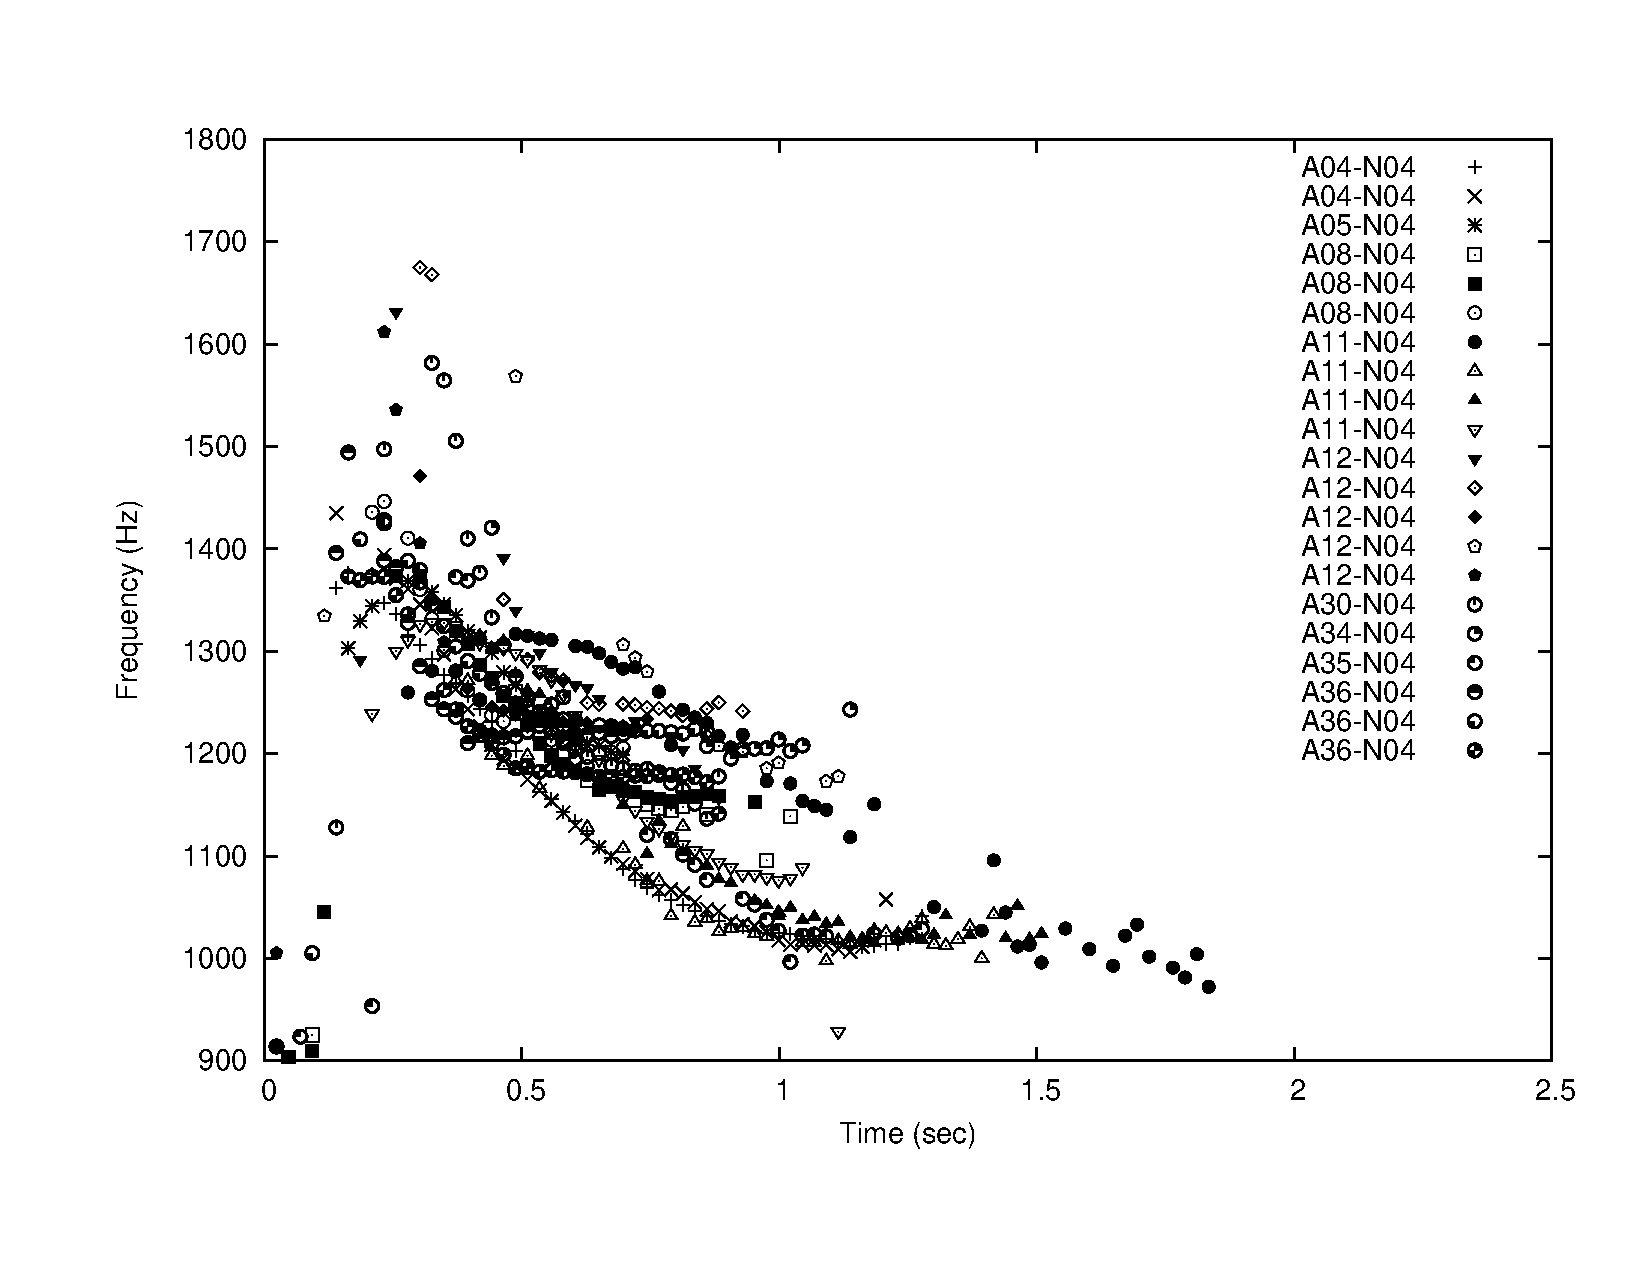
\includegraphics[width=90mm]{figures/pitch-N04}
%% \caption{F0 contour for 21 examples of the N04 call.}
%% \label{fig:pitch-N04}
%% \end{figure}

%% \begin{figure}[h]
%% \centering
%% 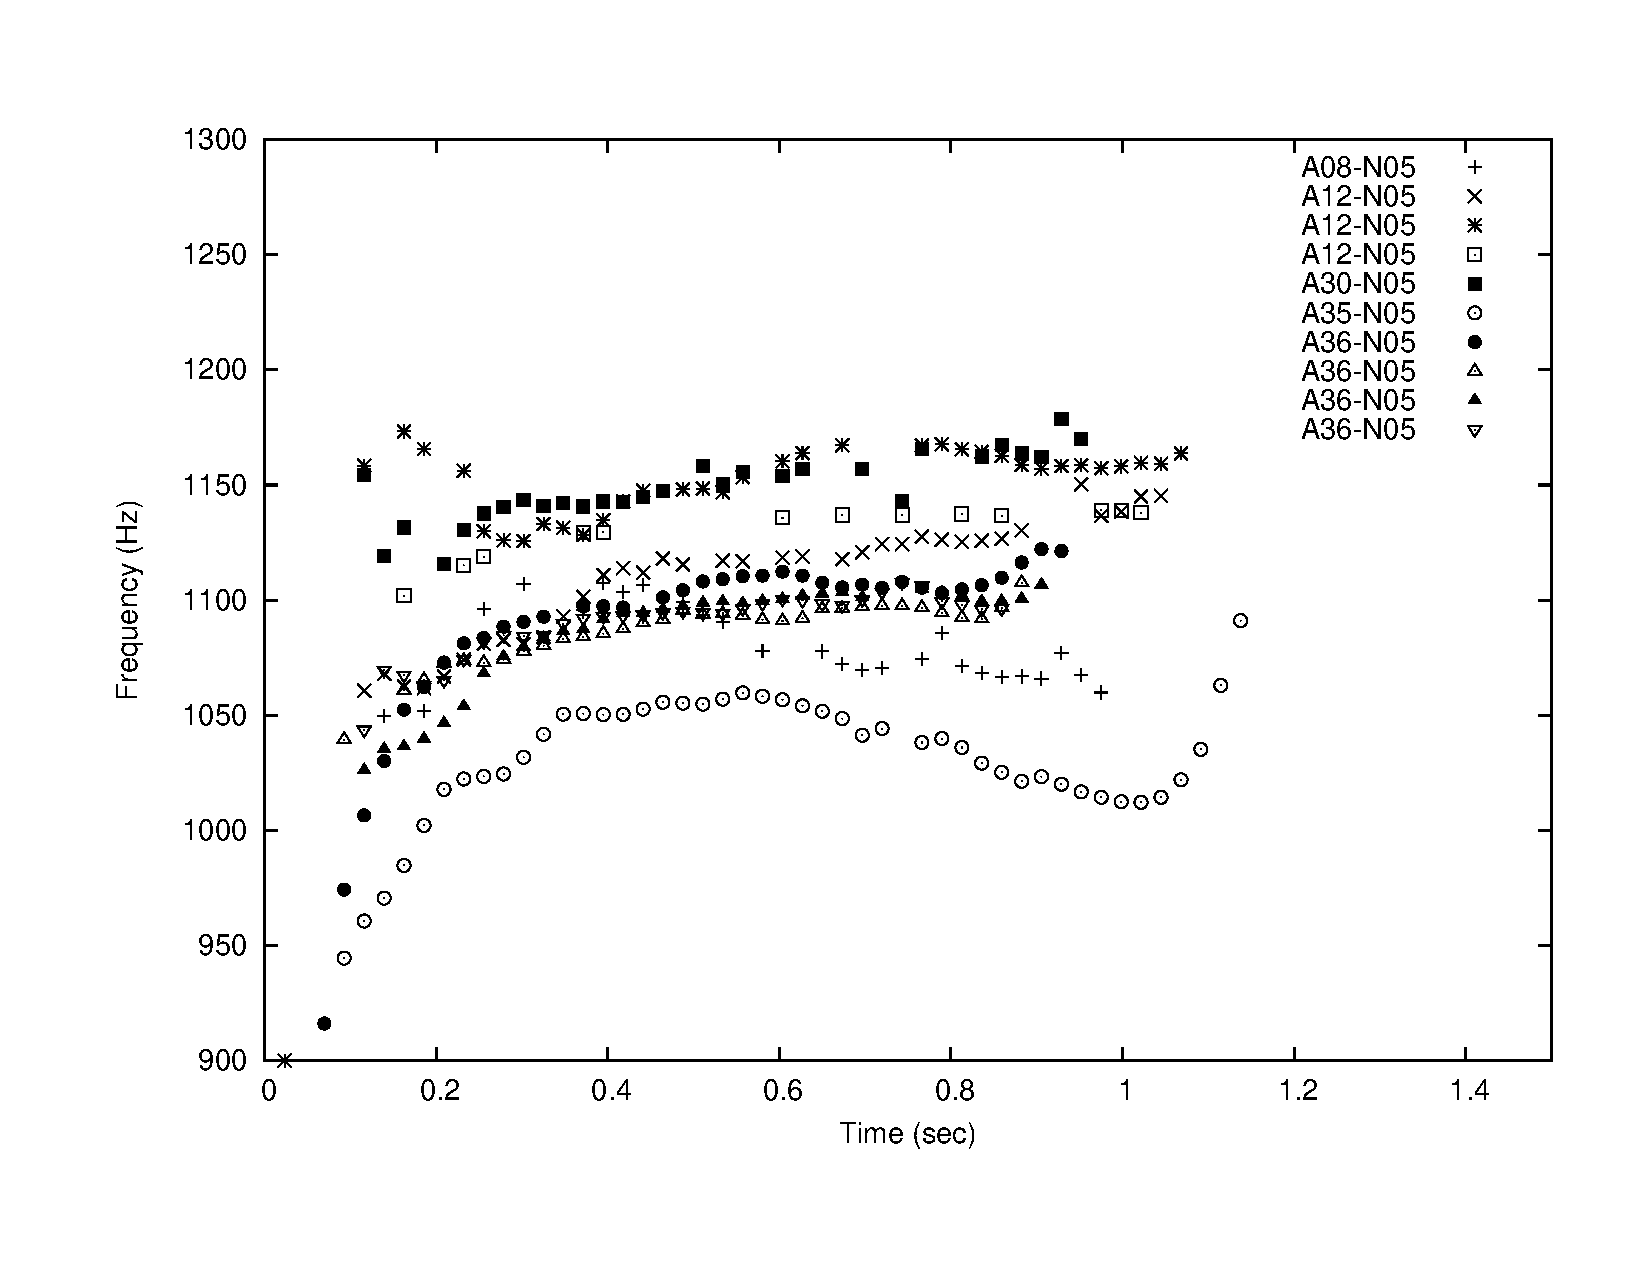
\includegraphics[width=90mm]{figures/pitch-N05}
%% \caption{F0 Contour for 10 examples of N05 call.}
%% \label{fig:pitch-N05}
%% \end{figure}

%% This approach is certainly valid if slope changes within a given
%% window characterize the signal well and the signal is fairly free of
%% noise. We therefore have examined SAX for a possible avenue to
%% transcribe Orca vocalizations. We determined, however, that
%% considering windowed slope fragments of Orca vocalizations does
%% produce sequences that are of lower quality than those produced by our
%% transcription technique which we refer to as FTSQ (Fundamental
%% Frequency Time Series Quantization).  The FTSQ procedure is outlined
%% in detail below. We do not provide classification results for SAX
%% sequences because the majority of SAX sequences were too long in order
%% to be processed by our dynamic programming based alignment algorithm
%% and hence a direct comparison can't be impartial. Further, we observed
%% that the fundamental frequency of Orca vocalizations carries a lot of
%% information, that is, it seems to be stable, and within a certain
%% range that is unique to a large portion of the vocalizations in our call
%% catalog. Since SAX is normalizing the signal slope within a sliding
%% window it cannot take advantage of this important feature.

%% \subsection{Signal Pre-processing and FTSQ}

%% Fundamental Frequency Time Series Quantization is a time series
%% quantization approach that transcribes an audio time series based on
%% an estimate of it's fundamental frequency ($F_0$).

%% In general it is not feasible to analyze Orca vocalizations as a raw
%% time series, since these signals are a complex mixture of sinusoids and
%% noise (see Figure \ref{fig:audio_raw}).  Figure \ref{fig:freqspec}
%% shows a spectrogram representation of the N01 and N09 Orca
%% vocalizations.  When comparing Figures \ref{fig:audio_raw} and
%% \ref{fig:freqspec} it is easy to see that the frequency components of
%% the audio signal reveals much more about the structure of the signal
%% than a raw audio time series by itself.

%% \begin{figure}[h]
%% \centering
%% 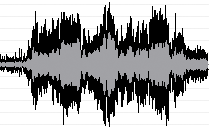
\includegraphics[width=0.4\columnwidth]{figures/audio_raw}
%% \caption{Raw audio signal of Orca vocalization N01.}
%% \label{fig:audio_raw}
%% \end{figure}
%% \begin{figure}[h]
%% \centering
%% 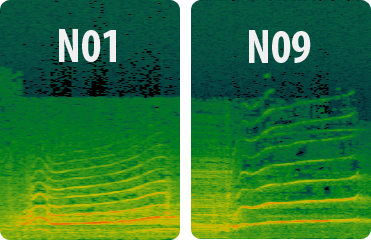
\includegraphics[width=0.60\columnwidth]{figures/freq_N01N09.png}
%% \caption{Frequency spectrum of Orca vocalizations N01 and N09.}
%% \label{fig:freqspec}
%% \end{figure}

%% Quantizing the fundamental frequency of an audio signal is am approach that makes 
%% use of the underlying structure in the frequency bands of the audio signal.
%% Loosely speaking one may think of the fundamental frequency as the pitch of a sound signal.
%% For our FTSQ technique we use Yin \cite{Cheveigne2002} a robust fundamental frequency 
%% estimation algorithm developed by Cheveigne et al.
%% Processing the audio waveform from Figure~\ref{fig:audio_raw} with Yin yields the 
%% fundamental frequency (in octaves relative to 440 Hz) shown in the top plot of Figure \ref{fig:yin}.
%% The two plots below the fundamental frequency show the aperiodicity and the
%% period-smoothed instantaneous power of the signal; they give estimate in the 
%% confidence on the approximation of $F_0$ and are used to identify meaningful
%% regions of interest within the $F_0$ signal.
%% \begin{figure}[h]
%% \centering
%% 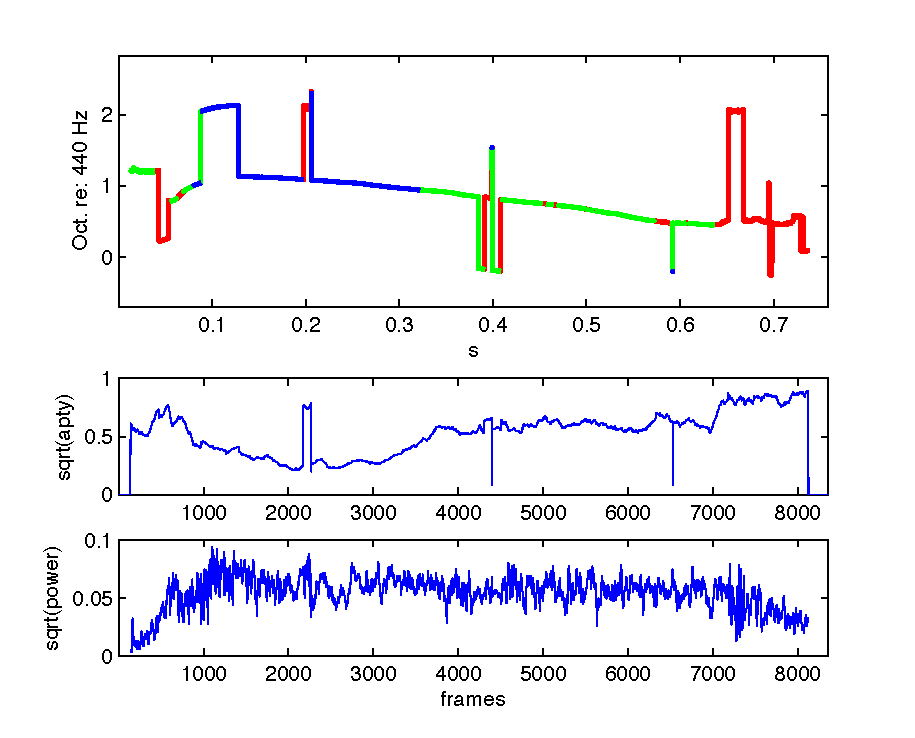
\includegraphics[width=\columnwidth]{figures/yin}
%% \caption{Frequency spectrum of Orca vocalizations N01 and N09}
%% \label{fig:yin}
%% \end{figure}


%% A further issue that is encountered commonly in the process of
%% determining a pitch contour for an audio recording is the optimization
%% of all the parameters of the pitch detection algorithm to perform well
%% on the particular dataset that is being used.  There are many such
%% parameters for each different algorithm, the important ones in the Yin
%% algorithm include the window size and hop size of the FFT, the high
%% and low frequency cutoffs, the high and low frequencies around which
%% the pitches will be wrapped using modulo arithmetic, the tolerance of
%% the Yin algorithm which determines which peaks in the autocorrelation
%% will be used for the pitch determination, the window size for the
%% median filter, and the number of histogram bins in which to divide the
%% frequency range into.  In our previous work, this was done by hand by
%% plotting points using MATLAB or Gnuplot, which can be a long and
%% labour intensive process.

%% For this project, we added custom visualization tools to our OpenMIR
%% platform to view the original audio as a spectrogram, to allow the
%% user to listen to this audio, to show a pitch contour with dynamic
%% controls over these various parameters, and an energy display that
%% shows the RMS energy of the audio signal.  This interface is shown in
%% Figure \ref{fig:openmir}.  This software allowed us to quickly
%% iterate over a large number of parameters, and to determine the
%% optimal parameters for the Yin algorithm.  The most important of these
%% was the median filter size, and a median filter of size 11 is shown in
%% Figure \ref{fig:openmir}.

%% \begin{figure}[t]
%% \centering
%% 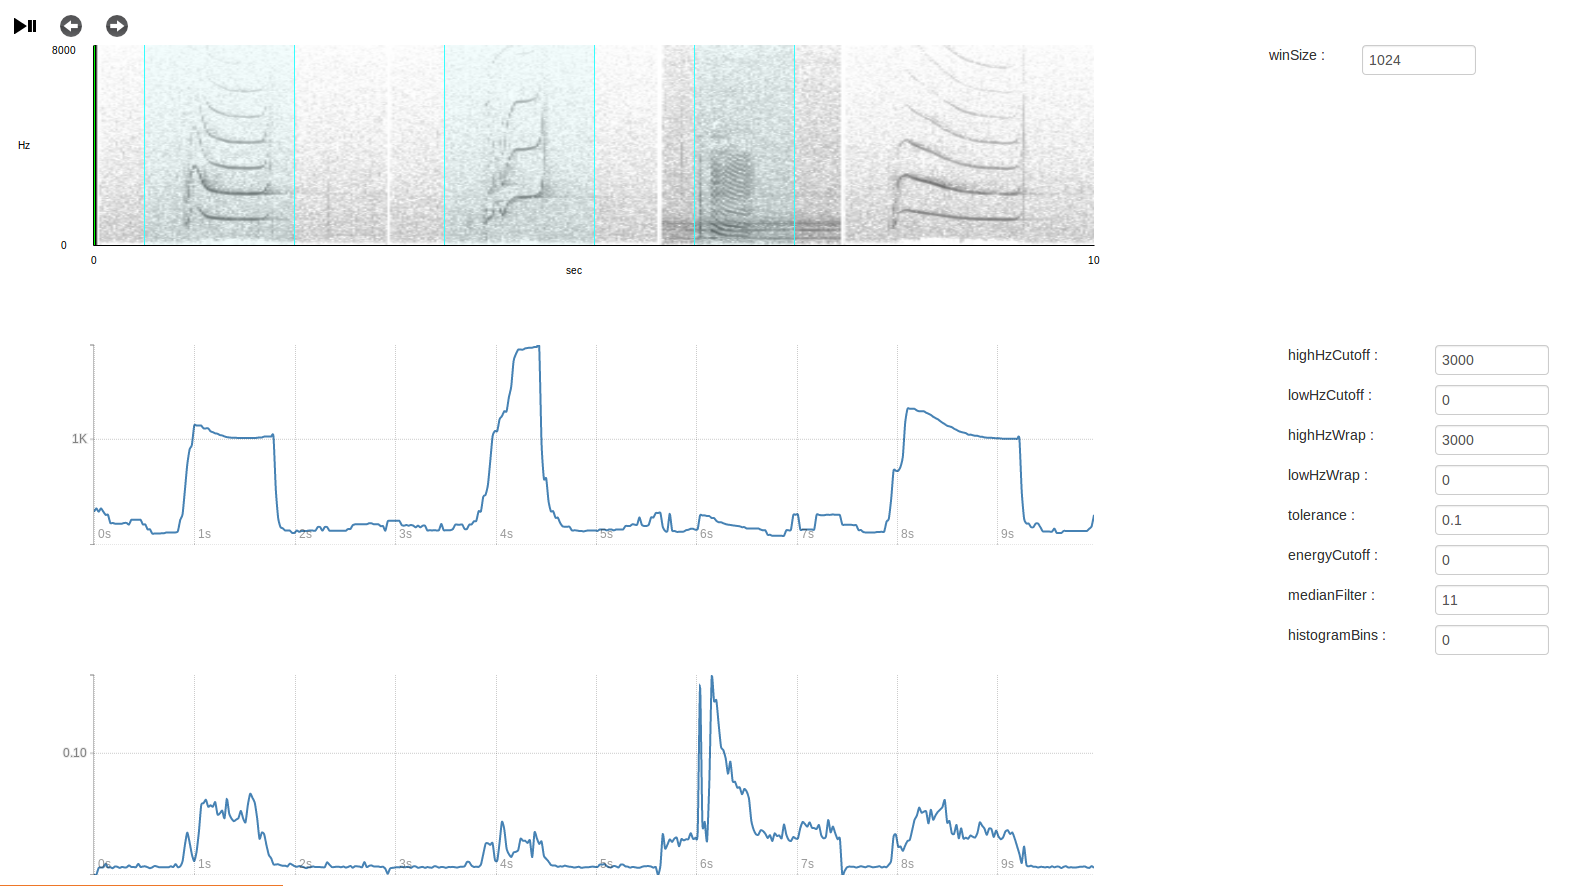
\includegraphics[width=\columnwidth]{figures/openmir}
%% \caption{Spectrogram, pitch and RMS view of a small portion of the Orchive
%% catalog viewed with the OpenMIR interface. }
%% \label{fig:openmir}
%% \end{figure}

%% \subsubsection{Octave Errors}
%% The output of Yin does not always give a proper estimate of $F_0$.
%% Indeed, the $F_0$ signal in Figure \ref{fig:yin} displays several
%% estimation errors that we herein refer to as \emph{octave errors}.
%% Octave errors manifest themselves as sudden jumps in a multiple of the
%% core $F_0$ frequency. Figure \ref{fig:yin} displays multiple octave
%% errors the first one at about 0.1 seconds. When quantizing the $F_0$
%% signal into a letter representation over a finite alphabet. Octave
%% errors result in mis-mapped letters in the output sequence. To a
%% certain degree we are able to handle octave errors by crafting a
%% custom substitution matrix in our sequence alignment
%% algorithm. However, doing so ultimately lowers the confidence in our
%% alignment score and might confuse legitimate frequency jumps with
%% octave errors and as a result would not penalize mismatches
%% appropriately. Therefore, we have developed a technique that can
%% automatically correct for the majority of octave errors and as a net
%% effect produces a more accurate letter representation.

%% We first run the $F_0$ signal obtained from Yin through a median filter, 
%% which smoothes the signal and eliminates small transients that occur due
%% to noise in the original signal. We then threshold the aperiodicity and the
%% period-smoothed instantaneous power to obtain $F_0$ signal regions at which
%% the $F_0$ signal is estimated with high confidence. After down-sampling the
%% signal we obtain the representation shown in Figure
%% \ref{fig:clean_yin}.

%% \begin{figure}[h]
%% \centering
%% 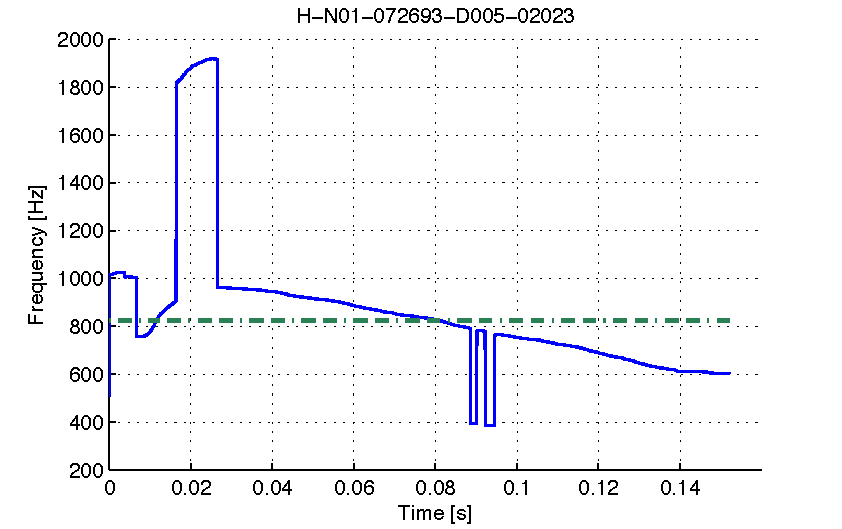
\includegraphics[width=\columnwidth]{figures/yin_clean}
%% \caption{Thresholded and down-sampled $F_0$ signal of a N01 call.}
%% \label{fig:clean_yin}
%% \end{figure}

%% The green line represents the median of the original $F_0$ signal
%% drawn in blue. The octave errors are clearly identifiable as such in
%% Figure \ref{fig:octave_yin} which shows versions of the $F_0$ signal
%% one octave above (purple) and on octave below (red) the original
%% (blue).  $F_0$ signal. To correct for octave errors we simply piece
%% the portions of the three versions of the $F_0$ signal together
%% according to which ever signal is closest to a slightly upwards biased
%% median of the original signal (blue). This yields the black $F_0$
%% curve wich shows the now automatically corrected version of the $F_0$
%% signal.
%% \begin{figure}[h]
%% \centering
%% 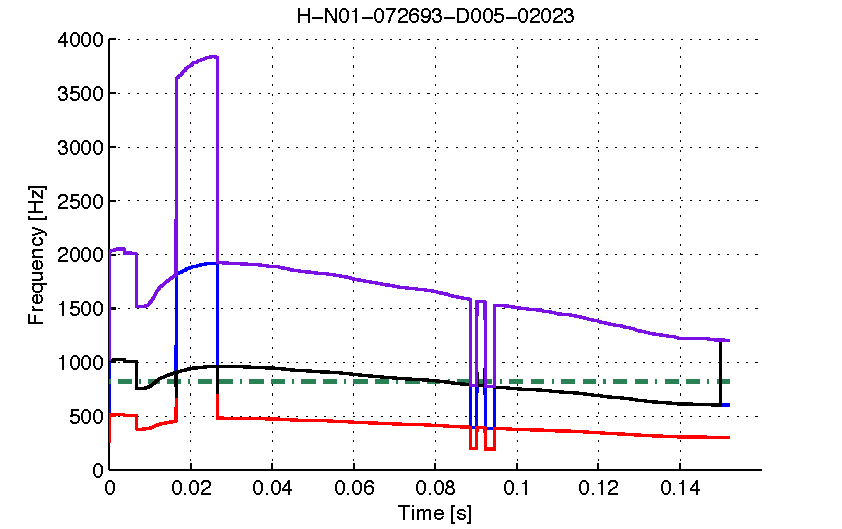
\includegraphics[width=\columnwidth]{figures/octave_fix}
%% \caption{Octave errors within a $F_0$ signal of a N01 call.}
%% \label{fig:octave_yin}
%% \end{figure}

%% \subsection{Log-Normal Signal Quantization}
%% When transcribing the $F_0$ signal into a letter representation suitable 
%% for sequence alignment tools it is natural to ask how these letters should be
%% assigned over the range of possible $F_0$ frequency values. A naive approach
%% would be to map $F_0$ frequencies to letters in a linear fashion. However, while
%% this approach does work well in practice, we investigated if a non-linear mapping
%% might potentially be more appropriate. For this purpose we plotted
%% the distribution of $F_0$ frequencies over time for the whole catalog of
%% Orca vocalizations in Figure \ref{fig:freq_dist}. The dynamic range of
%% $F_0$ incorporates frequencies from about 80 to 2400Hz, with three high density bands
%% at around 250, 700 and 1200Hz. Ideally one would therefore quantize the $F_0$ signal
%% using a three-modal distribution. However, for simplicity we chose a log-normal 
%% distribution (see Figure \ref{fig:log_norm}), which provides us with a fine resolution
%% for the more common $F_0$ frequencies and quantizes high $F_0$ frequencies at a coarser level.
%% \begin{figure}[h]
%% \centering
%% 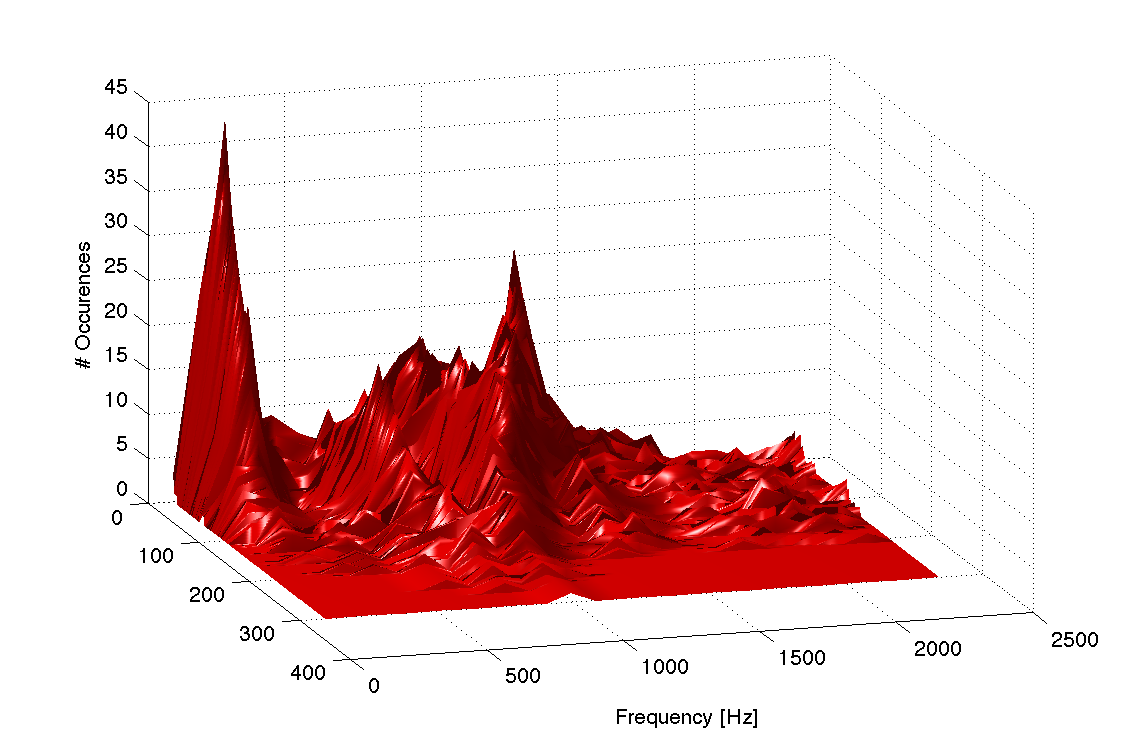
\includegraphics[width=\columnwidth]{figures/freq_dist}
%% \caption{Distribution of $F_0$ frequencies of call catalog.}
%% \label{fig:freq_dist}
%% \end{figure}

%% \begin{figure}[h]
%% \centering
%% 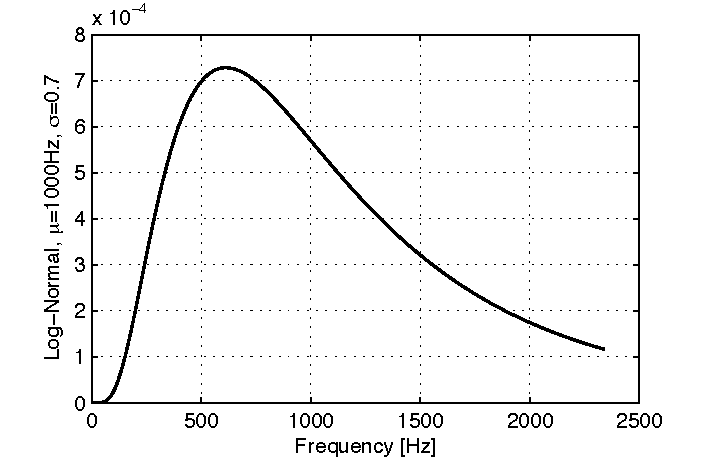
\includegraphics[width=0.7\columnwidth]{figures/log_norm}
%% \caption{Log-normal distribution for quantization}
%% \label{fig:log_norm}
%% \end{figure}

%% The result of log-normal quantization of the $F_0$ trace in Figure
%% \ref{fig:octave_yin} is provided in Figure
%% \ref{fig:letter_curve}. Finally, the resulting letter sequence is
%% given by \texttt{LLHHJJKKKKKKKKKKKKJJJJJJJII--IIIIIHHHHHHHGGGGGFFFFFF}
%% which can readily be consumed by a dynamic programming sequence
%% alignment algorithm.

%% \begin{figure}[h]
%% \centering
%% 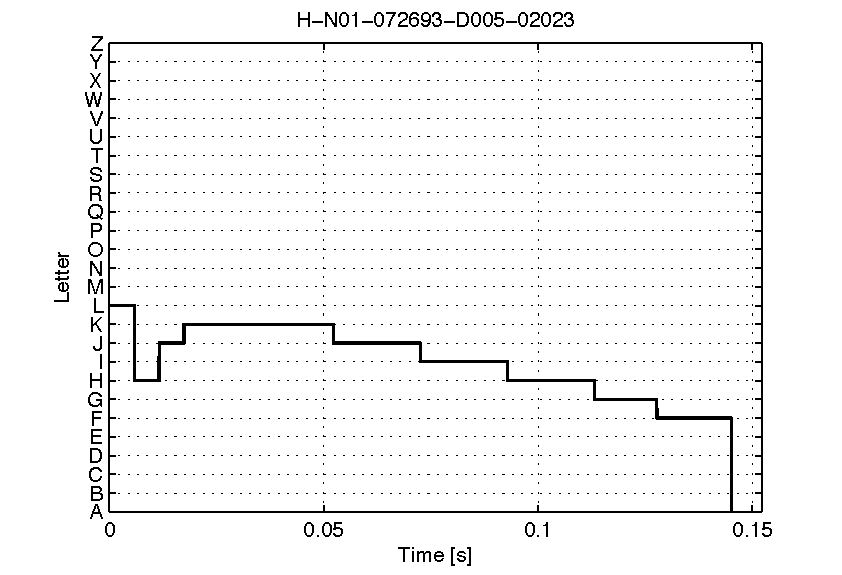
\includegraphics[width=\columnwidth]{figures/letter_curve}
%% \caption{$F_0$ signal of N01 call quantized to a finite alphabet}
%% \label{fig:letter_curve}
%% \end{figure}

%% \begin{table}
%% \centering
%% \begin{tabular}{|c|c|} 
%% \hline
%% Data Set                         &  Global Accuracy  \\
%% \hline
%% Original                         &              64\%  \\
%% Octave Removal - Linear          &              81\%  \\
%% Octave Removal - NonLinear 900   &              80\%  \\
%% Octave Removal - NonLinear 1200  &              81\%  \\
%% J48                              &              58\%  \\
%% Naive Bayes                      &              65\%  \\
%% SVM                              &              75\%  \\
%% \hline
%% \end{tabular}
%% \caption{Global accuracy for different methods of converting a Yin
%%   pitch contour into an alphabet using FTSQ}
%% \label{table:performance}
%% \end{table}


%% \begin{table}
%% \centering
%% \begin{tabular}{|c|c|} 
%% \hline
%%  Call  &  Accuracy  \\
%% \hline
%%  N47   &     0.400  \\
%%  N01   &     0.969  \\
%%  N12   &     0.583  \\
%%  N05   &     0.785  \\
%%  N04   &     1.000  \\
%%  N03   &      0.75  \\
%%  N09   &     0.772  \\
%% \hline
%% \end{tabular}
%% \caption{Global accuracy for different call types using Octave Removal
%%   NonLinear 1200 parameters with the FTSQ algorithm.}
%% \label{table:performance}
%% \end{table}

%% \section{Alphabetic Sequence Representation}

%% In order for sequence comparison algorithms to work well, it is
%% necessary that the combination of the letters and the scoring matrix
%% are compatible and output meaningful results.  In the two sections
%% below, we show the result of quantizing the signal using the nonlinear
%% histogram approach for two of the more common calls vocalized by
%% A-clan Northern Resident whales.  The first is the very common N4
%% call, which consists of a quick up swing in pitch, followed by a
%% downswing and then a constant tone.  In it we can clearly see long
%% regions of the repeated letters, P,O,N,M,L,K.  Even from a quick
%% visual inspection these repeated letters show that our method of
%% converting frequencies into a discrete alphabet is promising.

%% {\tiny
%% \begin{verbatim}
%% N04 A04 HIKNOOOOOPPPPOOOOOOOOOOOONNNNNNNNNNNNMMMMMMMMMMMMLLLLLLLLLLLLLLLLLLKKKKKKKKKKKKKKK
%% N04 A04 IJNOPPPPPPPPPPPOOOOOOOOONNNNNNNNMMMMMMMMMMMMMMLLLLLLLLLLLLLLLLLLLLLLKKKKKKKKKKKKKK
%% N04 A05 NLKLMNOOOOOOOOOOOOOOOOOOOOOOOOOONNNNNNNNNNNNNNNNNNNNMHGQ
%% N04 A08 RILMNNOOOOOOOOIIOOOOOOOOOOONNNNNNNNNNNNNNNNNNNNNMMMMMMMMMMMMMMMMMMMMMLLLLLLLMLLLLL
%% N04 A08 SIIJJKNPQQRPIIOOOOOOOONNNNNNNNNNNNNNMMMMMMMMMMMMMMMMMMMMMMMMMMDCCCMMM
%% \end{verbatim}
%% }

%% Even more promising were the results for another call, N5, which
%% consists of a constant tone.  These calls are from the A36 matriline
%% of orcas, which now consists of only two whales, the brothers A37 and
%% A46, although the grandmother whale, A12 often now associates with
%% this matriline after A34, her daughter's matriline, grew large in
%% size.  From these calls, we can see that the frequency represented by
%% the letter L is very constant throughout the entire call, and is a
%% clear indication that this is an N5 call.

%% {\tiny
%% \begin{verbatim}
%% N05,A36,A36-N05-070806-D012-13913,IIJJJKKKKKLLLLLLLLLLLLLLLLLLLLLLLLLLLLLLLLLLLLLLLLLLLLLL
%% N05,A36,A36-N05-070806-D012-13917,JJJKKLLFLLLLLLLLLLLLLLLLLLLLLLLLLLLLLLLLLLLLLLLLLLLLLLLL
%% N05,A36,A36-N05-070806-D012-13921,IIJJKKKKKKKKKLLLLLLLLLLLLGLLLLLLLLLLLLLLLLLLLLLLLLLLLLLL
%% N05,A36,A36-N05-071506-D017-11311,IQHJKLLLLLLLLLLLLLLLLLLLLLLLLLLLLLLLLLLLLLLLLLLLLLLLLLLL
%% \end{verbatim}
%% }



%%%%%%%%%%%%%%%%%%%%%%%%%%%%%%%%%%%%%%%%%%%%%%%%%%%%%%%%%%%%%%%%%%%%%%%%%%%%%%%%
%%%%%%%%%%%%%%%%%%%%%%%%%%%%%%%%%%%%%%%%%%%%%%%%%%%%%%%%%%%%%%%%%%%%%%%%%%%%%%%%
%% Chapter - Conclusions
%%%%%%%%%%%%%%%%%%%%%%%%%%%%%%%%%%%%%%%%%%%%%%%%%%%%%%%%%%%%%%%%%%%%%%%%%%%%%%%%
%%%%%%%%%%%%%%%%%%%%%%%%%%%%%%%%%%%%%%%%%%%%%%%%%%%%%%%%%%%%%%%%%%%%%%%%%%%%%%%%


\startchapter{Conclusions}
\label{chapter:conclusion}

conclusions



\section{Old}


\section{Future work}


There remains considerable work to be done in regards to the Orchive
as a whole.  The first is to find more examples of clear, nearby,
isolated orca vocalizations and background noise.  There are 12,000
annotations, about half of which are orca vocalizations.  A rough
estimate would be that about 1 in 20 of these would be a loud,
isolated vocalization, so one task we are working on is developing
tools to quickly let us go through the existing annotations and to
make training sets for Machine Learning algorithms.  In combination
with this is the task to better trim the ends of orca calls to
eliminate the silences that confound our Machine Learning algorithms.
We are developing HTML5 based tools to help us to manually do this,
and are also refining existing and developing new algorithms to
automatically do this.

The most exciting directly applicable future work to the current work
involves doing large scale clustering and vector quantization (VQ) on
the loud, isolated, orca vocalizations found in this study.  The VQ
algorithm will give us as output an alphabet with an arbitrary sized
dictionary.  With this one dimensional quantized and clustered
representation of the audio, we plan to use tools and techniques from
Bioinformatics \cite{sarkar2002} and Symbolic Aggregate Approximation
\cite{lin07} to extract information from this archive at a large scale.
Although this project concentrated on classification, it is the
clustering capabilities of Mahout that would be useful for this task,
and would be even more appropriate for doing large scale clustering
than for doing classification.

\section{Conclusions}

We set out to do two things, first, to assign audio features to the
entire Orchive, and further to classify all the audio in it into the
classes of ``orca'' and ``background''.  We achieved this by using the
Westgrid cluster and the bextract and sfplugin programs that are part
of Marsyas.  For the bextract part it took approximately 3 hours of
wall clock time, run on 37 computers to calculate all the features of
the Orchive.  For the sfplugin part, which classified the audio, we
ran on 42 nodes and it took 15 hours to annotate the entire archive.
This is an amazing speedup in itself, we had always considered that
calculating the features would take such a long time that we would at
least have to cache the intermediate features, but this assumption now
needs to be challenged.

The second thing we set out to do was to compare a variety of
distributed computing systems for both their performance and their
ease of use.  The simple Weka system on PBS was shockingly good, and
was extremely simple to setup and use.  With Weka, one is able to do a
wide variety of algorithms and to compare their results.  

Mahout is an excellent system, with many powerful capabilities and
with deep integration into Hadoop.  In our tests, we found the most
difficult thing as a student was to get the resources to run a
reasonably large (10-20 node) Hadoop cluster.  As we described in the
report, it is no small feat to get the Hadoop cluster installed and
running, especially on unknown hardware, but once this is done, Mahout
is simple to use and allows the storage of results on HDFS, the use of
which is almost essential, given the quantity of final and
intermediate results that need to be stored for a typical experimental
setup.  

Bextract in it's hybrid mode is perhaps the most useful system of this
entire group.  Because it does not need to generate intermediate
feature files that take huge amounts of disk space and often need to
be transferred to other computers to do the Machine Learning, it can
lead to a huge savings in time.  It is almost like having a mini
cluster within your one job, one where you do the feature extraction
and Machine Learning in one process.  All of the final classification
results that we ran were with this hybrid system.



\section{Future work}

There remains considerable work to be done in regards to the Orchive
as a whole.  The first is to find more examples of clear, nearby,
isolated orca vocalizations and background noise.  There are 12,000
annotations, about half of which are orca vocalizations.  A rough
estimate would be that about 1 in 20 of these would be a loud,
isolated vocalization, so one task we are working on is developing
tools to quickly let us go through the existing annotations and to
make training sets for Machine Learning algorithms.  In combination
with this is the task to better trim the ends of orca calls to
eliminate the silences that confound our Machine Learning algorithms.
We are developing HTML5 based tools to help us to manually do this,
and are also refining existing and developing new algorithms to
automatically do this.

The most exciting directly applicable future work to the current work
involves doing large scale clustering and vector quantization (VQ) on
the loud, isolated, orca vocalizations found in this study.  The VQ
algorithm will give us as output an alphabet with an arbitrary sized
dictionary.  With this one dimensional quantized and clustered
representation of the audio, we plan to use tools and techniques from
Bioinformatics \cite{sarkar2002} and Symbolic Aggregate Approximation
\cite{lin07} to extract information from this archive at a large scale.
Although this project concentrated on classification, it is the
clustering capabilities of Mahout that would be useful for this task,
and would be even more appropriate for doing large scale clustering
than for doing classification.


%%%%%%%%%%%%%%%%%%%%%%%%%%%%%%%%%%%%%%%%%%%%%%%%%%%%%%%%%%%%%%%%%%%%%%%%%%%%%%%%
%%%%%%%%%%%%%%%%%%%%%%%%%%%%%%%%%%%%%%%%%%%%%%%%%%%%%%%%%%%%%%%%%%%%%%%%%%%%%%%%
%% Chapter - Glossary
%%%%%%%%%%%%%%%%%%%%%%%%%%%%%%%%%%%%%%%%%%%%%%%%%%%%%%%%%%%%%%%%%%%%%%%%%%%%%%%%
%%%%%%%%%%%%%%%%%%%%%%%%%%%%%%%%%%%%%%%%%%%%%%%%%%%%%%%%%%%%%%%%%%%%%%%%%%%%%%%%

\startchapter{Glossary}
\label{chapter:glossary}

ANOVA (Science) - Analysis of Variance between groups - A group of statistical techniques to test hypotheses based on experimental results.  It tests the distribution of the means of variables to see if they are the same, assuming the variables are normally distributed.
\\

Cross-validation (Computer Science) - A method used to test the accuracy of machine learning classifiers by separating a dataset into examples used to train the classifier and examples used to test the classifier.
\\

Ethnomusicology (Musicology) - a sub-discipline of Musicology that focuses on the study of the socio-cultural aspects of music in societies around the world.
\\

Folksonomy (Computer Science) - a system of classification that comes from a group of users collaboratively creating and managing tags in an effort to annotate and categorize content
\\

Flux (MIR) - In this work, is the norm of the difference vector between two successive magnitue/power spectra.
\\

MFCC coefficients (MIR) - A way to transform a standard spectrum into one that more closely approximates how the human ear perceives sound.
\\
Music Information Retrieval (Computer Science) - also known by the acronym MIR, a new field of study where one applies tools from areas such as Digital Signal Processing, Audio Feature Extraction and Machine Learning to help people understand and retrieve information from music or audio.
\\

Ontology (Computer Science) - a formal representation of ideas or concepts and the relation between them.  This Computer Science definition of ontology is a subset of the broader philosophical idea of ontology, which is a study of what exists and what can exist.
\\

Rolloff (MIR) - A measure of the steepness of falloff in an audio spectrum
\\


Self-Organizing Map (Computer Science) - A technique that maps a high
dimensional feature space to a lower space.  It is a similar technique
to artifical neural networks.

Spectral Centroid (MIR) - A measure of the ``center of mass'' of a spectrum.
\\


XML (Computer Science) - eXtensible Markup Language - A popular
tree-tree based format for encoding data

JSON - Javascript Object Notation.  A modern data-exchange format,
used extensively as a way for servers to send data to web-based
clients.

Redis - A modern key-value object store designed to primarily hold all
it's data in memory to facilitate fast retrieval by clients.  

Syrinx - One of the structures in birds that is used to produce sound

Phonic Lips - Also known as ``museau de singe'' or ``monkey lips'' -
The mechanism by which odontocetes produce sound

Odontocete - A suborder of cetaceans of which one of the
distinguishing features is they have teeth, in contrast to the
Mysticeti, which have baleen

Mysticeti - A suborder of cetaceans of which one of the distinguishing
features is they use baleen to filter prey from the water, in contrast
to the Odontocetes, which have teeth

%%%%%%%%%%%%%%%%%%%%%%%%%%%%%%%%%%%%%%%%%%%%%%%%%%%%%%%%%%%%%%%%%%%%%%%%%%%%%%%%
%%%%%%%%%%%%%%%%%%%%%%%%%%%%%%%%%%%%%%%%%%%%%%%%%%%%%%%%%%%%%%%%%%%%%%%%%%%%%%%%
%% Chapter - Web Links
%%%%%%%%%%%%%%%%%%%%%%%%%%%%%%%%%%%%%%%%%%%%%%%%%%%%%%%%%%%%%%%%%%%%%%%%%%%%%%%%
%%%%%%%%%%%%%%%%%%%%%%%%%%%%%%%%%%%%%%%%%%%%%%%%%%%%%%%%%%%%%%%%%%%%%%%%%%%%%%%%

\startchapter{Web Links}
\label{chapter:weblinks}

The following are web links to the various web-based tools developed
in the course of this research:
\\

Cantillion : \url{http://cantillion.sness.net}.
\\

Orchive : \url{http://orchive.cs.uvic.ca}
\\

Audioscapes : \url{http://audioscapes.sness.net}
\\


%%%%%%%%%%%%%%%%%%%%%%%%%%%%%%%%%%%%%%%%%%%%%%%%%%%%%%%%%%%%%%%%%%%%%%%%%%%%%%%%
%%%%%%%%%%%%%%%%%%%%%%%%%%%%%%%%%%%%%%%%%%%%%%%%%%%%%%%%%%%%%%%%%%%%%%%%%%%%%%%%
%% Chapter - Publications
%%%%%%%%%%%%%%%%%%%%%%%%%%%%%%%%%%%%%%%%%%%%%%%%%%%%%%%%%%%%%%%%%%%%%%%%%%%%%%%%
%%%%%%%%%%%%%%%%%%%%%%%%%%%%%%%%%%%%%%%%%%%%%%%%%%%%%%%%%%%%%%%%%%%%%%%%%%%%%%%%

\startchapter{Publications from this Research}
\label{chapter:publications}

Presented here is a list of all the publications that come from the
research presented in this thesis:
\\

Steven R. Ness, Daniel Peter Biro and George Tzanetakis
Computer-assisted cantillation and chant research using content-aware
web visualization tools, Multimedia Tools and Applications, Accepted
for publication
\\

S. R. Ness, A. Theocharis, G. Tzanetakis, L. G. Martins Improving
Automatic Music Tag Annotation Using Stacked Generalization Of
Probabilistic SVM Outputs, ACM Multimedia 2009
\\

Steven R. Ness, George Tzanetakis, Audioscapes: exploring surface
interfaces for music exploration - ICMC 2009
\\

Steven R. Ness, George Tzanetakis, SOMba : Multiuser music creation
using Self-Organizing Maps and motion tracking - ICMC 2009
\\

Steven R. Ness, Daniel Peter Biro, George Tzanetakis : Content-aware
web browsing and visualization tools for cantillation and chant
research, 7th International Workshop on Content-Based Multimedia
Indexing
\\

George Tzanetakis, Manjinder Singh Benning, Steven R. Ness, Darren
Minifie, Nigel Livingston : Assistive Music Browsing using
Self-Organizing Maps - PETRA 2009 : 2nd International Conference on
PErvasive Technologies Related to Assistive Environments
\\

Steven R. Ness, Matthew Wright, Luis Gustavo Martins, George
Tzanetakis: Chants and Orcas: semi-automatic tools for audio
annotation and analysis in niche domains. ACM Multimedia 2008: 9-16
\\

Daniel Peter Biro, Steven Ness, Matthew Wright, W. Andrew Schloss and
George Tzanetakis Decoding the Song: Histogram-Based Paradigmatic and
Syntagmatic Analysis of Melodic Formulae in Hungarian Laments, Jewish
Torah Trope, Tenth Century Plainchant and Koran Recitation EMUS
Expressivity in MUsic and Speech : IRCAM - Institut de Recherche et de
Coordination Acoustique/Musique - Paris, France
\\


\TOCadd{Bibliography}
\bibliographystyle{alpha}
\bibliography{thesis}




\end{document}
